%%%%%%%%%%%%%%%%%%%%%%%%%%%%%%%%%%%%%%%%%
% Tufte-Style Book (Minimal Template)
% LaTeX Template
% Version 1.0 (5/1/13)
%
% This template has been downloaded from:
% http://www.LaTeXTemplates.com
% License:
% CC BY-NC-SA 3.0 (http://creativecommons.org/licenses/by-nc-sa/3.0/)
%
% IMPORTANT NOTE:
% In addition to running BibTeX to compile the reference list from the .bib
% file, you will need to run MakeIndex to compile the index at the end of the
% document.
%
%%%%%%%%%%%%%%%%%%%%%%%%%%%%%%%%%%%%%%%%%

%----------------------------------------------------------------------------------------
%	PACKAGES AND OTHER DOCUMENT CONFIGURATIONS
%----------------------------------------------------------------------------------------

\documentclass{tufte-book}\usepackage[]{graphicx}\usepackage[]{color}
%% maxwidth is the original width if it is less than linewidth
%% otherwise use linewidth (to make sure the graphics do not exceed the margin)
\makeatletter
\def\maxwidth{ %
  \ifdim\Gin@nat@width>\linewidth
    \linewidth
  \else
    \Gin@nat@width
  \fi
}
\makeatother

\definecolor{fgcolor}{rgb}{0.345, 0.345, 0.345}
\newcommand{\hlnum}[1]{\textcolor[rgb]{0.686,0.059,0.569}{#1}}%
\newcommand{\hlstr}[1]{\textcolor[rgb]{0.192,0.494,0.8}{#1}}%
\newcommand{\hlcom}[1]{\textcolor[rgb]{0.678,0.584,0.686}{\textit{#1}}}%
\newcommand{\hlopt}[1]{\textcolor[rgb]{0,0,0}{#1}}%
\newcommand{\hlstd}[1]{\textcolor[rgb]{0.345,0.345,0.345}{#1}}%
\newcommand{\hlkwa}[1]{\textcolor[rgb]{0.161,0.373,0.58}{\textbf{#1}}}%
\newcommand{\hlkwb}[1]{\textcolor[rgb]{0.69,0.353,0.396}{#1}}%
\newcommand{\hlkwc}[1]{\textcolor[rgb]{0.333,0.667,0.333}{#1}}%
\newcommand{\hlkwd}[1]{\textcolor[rgb]{0.737,0.353,0.396}{\textbf{#1}}}%

\usepackage{framed}
\makeatletter
\newenvironment{kframe}{%
 \def\at@end@of@kframe{}%
 \ifinner\ifhmode%
  \def\at@end@of@kframe{\end{minipage}}%
  \begin{minipage}{\columnwidth}%
 \fi\fi%
 \def\FrameCommand##1{\hskip\@totalleftmargin \hskip-\fboxsep
 \colorbox{shadecolor}{##1}\hskip-\fboxsep
     % There is no \\@totalrightmargin, so:
     \hskip-\linewidth \hskip-\@totalleftmargin \hskip\columnwidth}%
 \MakeFramed {\advance\hsize-\width
   \@totalleftmargin\z@ \linewidth\hsize
   \@setminipage}}%
 {\par\unskip\endMakeFramed%
 \at@end@of@kframe}
\makeatother

\definecolor{shadecolor}{rgb}{.97, .97, .97}
\definecolor{messagecolor}{rgb}{0, 0, 0}
\definecolor{warningcolor}{rgb}{1, 0, 1}
\definecolor{errorcolor}{rgb}{1, 0, 0}
\newenvironment{knitrout}{}{} % an empty environment to be redefined in TeX

\usepackage{alltt} % Use the tufte-book class which in turn uses the tufte-common class

\usepackage{microtype} % Improves character and word spacing
\usepackage{amsmath}
\usepackage{booktabs} % Better horizontal rules in tables
\usepackage[tikz]{bclogo}

%\usepackage{Sweave}
\usepackage{float}
\usepackage{graphicx} % Needed to insert images into the document 
\graphicspath{{graphics/}} % Sets the default location of pictures
\setkeys{Gin}{width=\linewidth,totalheight=\textheight,keepaspectratio} % Improves figure scaling
\usepackage{fancyvrb} % Allows customization of verbatim environments
\fvset{fontsize=\normalsize} % The font size of all verbatim text can be changed here

\newcommand{\hangp}[1]{\makebox[0pt][r]{(}#1\makebox[0pt][l]{)}} % New command to create parentheses around text in tables which take up no horizontal space - this improves column spacing
\newcommand{\hangstar}{\makebox[0pt][l]{*}} % New command to create asterisks in tables which take up no horizontal space - this improves column spacing

\usepackage{xspace} % Used for printing a trailing space better than using a tilde (~) using the \xspace command

\newcommand{\monthyear}{\ifcase\month\or January\or February\or March\or April\or May\or June\or July\or August\or September\or October\or November\or December\fi\space\number\year} % A command to print the current month and year


\newcommand{\blankpage}{\newpage\hbox{}\thispagestyle{empty}\newpage} % Command to insert a blank page

\newcommand{\newfun}[1]{\begin{LARGE} \begin{center} \texttt{#1} \end{center} \end{LARGE}}
\setcounter{tocdepth}{1}
\usepackage{makeidx} % Used to generate the index
\makeindex % Generate the index which is printed at the end of the document

%----------------------------------------------------------------------------------------
%	BOOK META-INFORMATION
%----------------------------------------------------------------------------------------

\title{YaRrr! The Pirate's Guide to R}

\author{Dr. Nathaniel D. Phillips}

%\publisher{Publisher Name}

%----------------------------------------------------------------------------------------
\IfFileExists{upquote.sty}{\usepackage{upquote}}{}
\begin{document}

% \begin{center}
% 
\includegraphics[width=40cm]{/Users/Nathaniel/Dropbox/Git/YaRrr_Book/media/YaRrr_Cover.pdf}
% \end{center}
% 


\frontmatter

\maketitle

%----------------------------------------------------------------------------------------
%	COPYRIGHT PAGE
%----------------------------------------------------------------------------------------

\newpage
\begin{fullwidth}
~\vfill
\thispagestyle{empty}
\setlength{\parindent}{0pt}
\setlength{\parskip}{\baselineskip}
Copyright \copyright\ \the\year\ \thanklessauthor

\par\smallcaps{Published by \thanklesspublisher}

\par\smallcaps{\url{http://www.nathanieldphillips.com}}

\par This document may not be used for any commercial purposes. All rights are reserved by Nathaniel Phillips.\index{license}

\par\textit{First printing, \monthyear}
\end{fullwidth}

%----------------------------------------------------------------------------------------

\tableofcontents % Print the table of contents

%----------------------------------------------------------------------------------------

%\listoffigures % Print a list of figures

%----------------------------------------------------------------------------------------

%\listoftables % Print a list of tables

%----------------------------------------------------------------------------------------
%	DEDICATION PAGE
%----------------------------------------------------------------------------------------

\cleardoublepage
~\vfill
\begin{doublespace}
\noindent\fontsize{18}{22}\selectfont\itshape
\nohyphenation
This book is dedicated to my former statistics instructors Dr. Thomas Moore and Dr. Wei Lin who taught me everything I know about statistics, and my PhD colleagues Dr. Dirk Wulff and Dr. Stefan Herzog who taught me everything I know about R.
\end{doublespace}
\vfill
\vfill


%----------------------------------------------------------------------------------------
%	INTRODUCTION
%----------------------------------------------------------------------------------------

%\cleardoublepage

\chapter{Introduction} % The asterisk leaves out this chapter from the table of contents

\subsection{Who am I?}

I am a pirate on the Bodensee in Konstanz Germany. When I started pirate training, I discovered R and have been hooked ever since. I'm now on a mission to convince everyone I can to make the switch from SPSS (or Excel, Matlab, JMP...) to R.

\subsection{This book is in progress..}

If you haven't figured it out already, this book is very much a work in progress. I'm constantly experimenting with the material and the layout. If you have any recommendations for changes or spot any errors, please write me at YaRrr.Book@gmail.com or tweet me @YaRrrBook

\marginnote{Email me with comments, recommendations or typos at: YaRrr.Book@gmail.com or tweet me at @YaRrrBook}

\subsection{Who is this book for?}
Anyone who wants to learn R can benefit from this book. I will assume that you have taken an introductory course in statistics, but have no substantial programming experience. While the techniques in this book apply to most data analysis problems, because my background is in experimental psychology I will cater the course to solving analysis problems commonly faced in psychological research.

\subsection{What this book \textbf{is}}

This book is meant to introduce you to the basic analytical tools in R, from basic coding and analyses, to data wrangling, plotting, and statistical inference.

\subsection{What this book is \textbf{not}}

This book does not cover any one topic in extensive detail. If you are interested in conducting analyses or creating plots not covered in the book, I'm sure you'll find the answer with a quick Google search!

\subsection{Why is R so great?}

As you've already gotten this book, you probably already have some idea why R is so great. However, in order to help prevent you from giving up the first time you run into a programming wall, let me give you a few more reasons:

\begin{enumerate}

\item R is 100\% free and as a result, has a huge support community. Unlike SPSS, Matlab, Excel and JMP, R is, and always will be completely free. This doesn't just help your wallet - it means that a huge community of R programmers will constantly develop an distribute new R functionality and packages at a speed that leaves all those other packages in the dust! Unlike Fight Club, the first rule of R is "Do talk about R!" The size of the R programming community is staggering. If you ever have a question about how to implement something in R, a quick Poogle\footnote{I am in the process of creating Poogle - Google for Pirates. Kickstarter page coming soon...} search will lead you to your answer virtually every single time.

\item R is incredibly versatile. You can use R to do everything from calculating simple summary statistics, to performing complex simulations to creating gorgeous plots like the chord diagram in Figure~\ref{fig:chorddiagram}. If you can imagine an analytical task, you can almost certainly implement it in R.

\begin{marginfigure}
\begin{tiny}
\begin{knitrout}
\definecolor{shadecolor}{rgb}{0.969, 0.969, 0.969}\color{fgcolor}\begin{kframe}
\begin{alltt}
\hlkwd{require}\hlstd{(}\hlstr{"circlize"}\hlstd{)}
\end{alltt}


{\ttfamily\noindent\itshape\color{messagecolor}{\#\# Loading required package: circlize}}\begin{alltt}
\hlstd{mat} \hlkwb{=} \hlkwd{matrix}\hlstd{(}\hlkwd{sample}\hlstd{(}\hlnum{1}\hlopt{:}\hlnum{100}\hlstd{,} \hlnum{18}\hlstd{,} \hlkwc{replace} \hlstd{=} \hlnum{TRUE}\hlstd{),} \hlnum{3}\hlstd{,} \hlnum{6}\hlstd{)}
\hlkwd{rownames}\hlstd{(mat)} \hlkwb{=} \hlstd{letters[}\hlnum{1}\hlopt{:}\hlnum{3}\hlstd{]}
\hlkwd{colnames}\hlstd{(mat)} \hlkwb{=} \hlstd{LETTERS[}\hlnum{1}\hlopt{:}\hlnum{6}\hlstd{]}
\hlkwd{chordDiagram}\hlstd{(mat)}
\end{alltt}
\end{kframe}
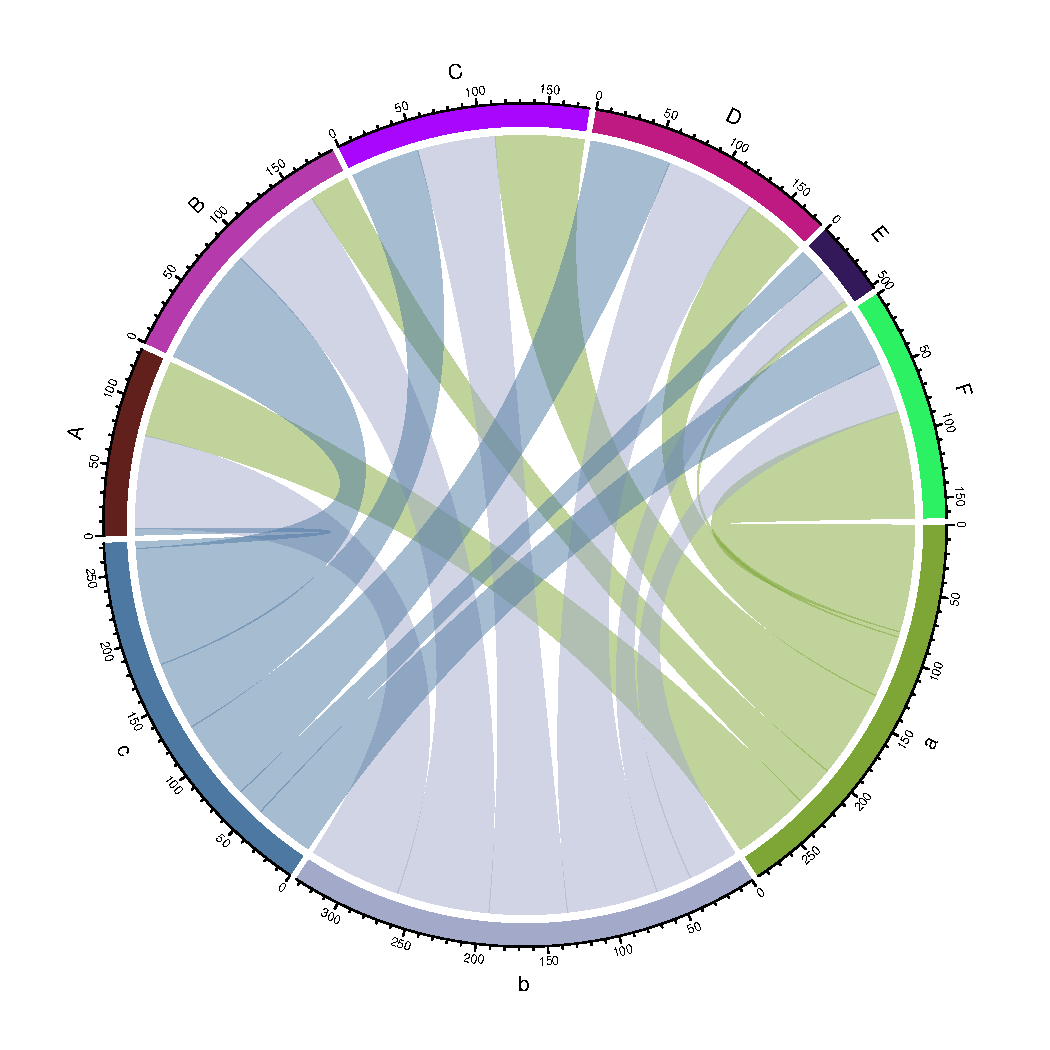
\includegraphics[width=\maxwidth]{figure/unnamed-chunk-1-1} 

\end{knitrout}
\end{tiny}
\caption{This is a \texttt{chordDiagram} plot that comes with the R package \texttt{circlize}.}
\label{fig:chorddiagram}
\end{marginfigure}


\item Using RStudio, You can easily and seamlessly combine R code, analyses, plots, and written text into elegant documents all in one place using Sweave (R and Latex) or RMarkdown. In fact, I wrote this entire book (the text, formatting, plots, code...yes, everything) in RStudio using Sweave. With RStudio and Sweave, instead of trying to manage two or three programs, say Excel, Word and (sigh) SPSS, where you find yourself spending half your time copying, pasting and formatting data, images and test, you can do everything in one place so nothing gets misread, mistyped, or forgotten.

\item Analyses conducted in R are transparent, easily shareable, and reproducible. If you ask an SPSS user how they conducted a specific analyses, they will either A) Not remember,  B) Try (nervously) to construct an analysis procedure on the spot that makes sense - which may or may not correspond to what they actually did months or years ago, or C) Ask you what you are doing in their kitchen\footnote{Get used to the bad jokes people. Lots more where that came from.}. I used to primarily use SPSS, so I speak from experience on this. If you ask an R user (who uses good programming techniques!) how they conducted an analysis, they should always be able to show you the exact code they used. Of course, this doesn't mean that they used the appropriate analysis or interpreted it correctly, but with all the original code, any problems should be completely transparent!

\item And most importantly of all, R is the programming language of choice for pirates, (who prefer the "YaRrr!" pronunciation)

\end{enumerate}

\subsection{Code Chunks}

In this book, R code is (almost) always presented in a separate gray box like this one:

\begin{footnotesize}
\begin{knitrout}
\definecolor{shadecolor}{rgb}{0.969, 0.969, 0.969}\color{fgcolor}\begin{kframe}
\begin{alltt}
\hlstd{a} \hlkwb{<-} \hlnum{1} \hlopt{+} \hlnum{2} \hlopt{+} \hlnum{3} \hlopt{+} \hlnum{4} \hlopt{+} \hlnum{5}
\hlstd{a}
\end{alltt}
\begin{verbatim}
## [1] 15
\end{verbatim}
\end{kframe}
\end{knitrout}
\end{footnotesize}

This is called a \textit{code chunk}. You should always be able to directly copy and paste code chunks directly into R. If you copy a chunk and it does not work for you, it is most likely because the code refers to a package, function, or object that I defined in a previous chunk. If so, read back and look for a previous chunk that contains the missing definition. As you'll soon learn, lines that begin with \texttt{\#} are either comments or output from prior code that R will ignore.

As you'll notice, I'll include code chunks before all plots in the book. In early chapters, the code might not make sense just yet. However, I elected to always include plotting code so you have the option of re-creating (and tweaking) any plot in the book.

\subsection{Additional Tips}

Because this is a beginner's book, I try to avoid bombarding you with too many details and tips when I first introduce a function. For this reason, at the end of every chapter, I present several tips and tricks that I think most R users should know once they get comfortable with the basics. I highly encourage you to read these additional tips as I expect you'll find at least some of them very useful if not invaluable.


\mainmatter


%----------------------------------------------------------------------------------------
%	CHAPTER 1
%----------------------------------------------------------------------------------------
\chapter{1: Installing R, RStudio, and the pirate dataset}
\label{ch:1}

%------------------------------------------------

Now that I've convinced you to use R, let's get started! First, you'll need to install the base R software.

1. Download and install the base R software (around 50mb)
    + Windows <http://cran.r-project.org/bin/windows/base/>
    + Mac <http://cran.r-project.org/bin/macosx/>

See Figure \ref{fig:rscreenshot} Here's how the base R software looks (on Mac). As you can see, it's very much a bare-bones software - just how we want it! No extra gimmicks or flashy bloatware needed!

\begin{marginfigure}
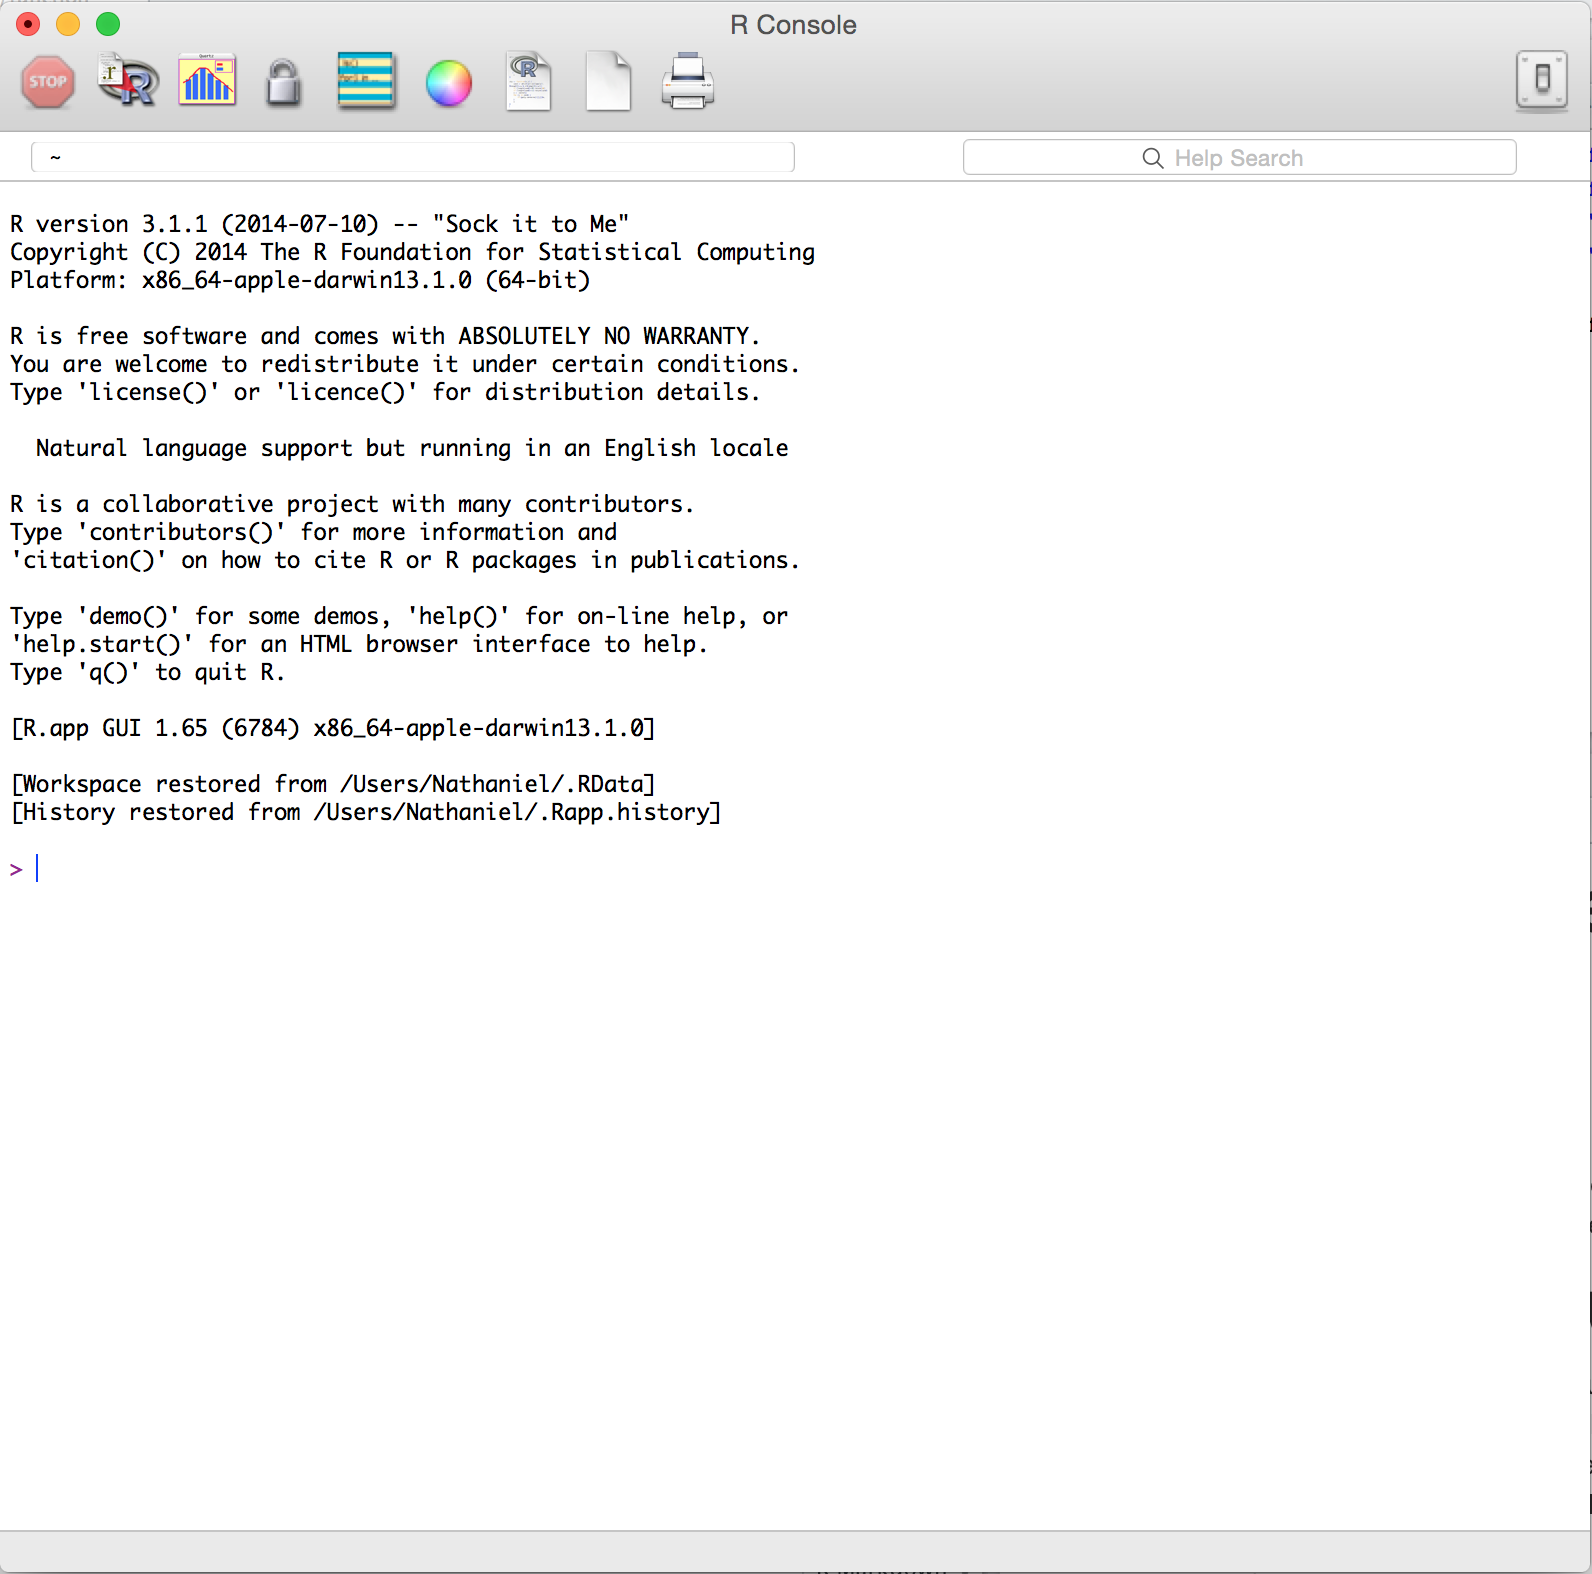
\includegraphics[width=\linewidth]{/Users/Nathaniel/Dropbox/Git/YaRrr_Book/media/RScreenshot.png}
\caption{Here is how the standard R application looks. Not too exciting - just how we like it!}
\label{fig:rscreenshot}
\end{marginfigure}

While you can do pretty much everything you want within base R, you'll find that most people these days do their R programming in an application called RStudio. RStudio is a graphical user interface (GUI)-like interface for R that makes programming in R a bit easier. To download and install RStudio (around 40mb), go to <http://www.rstudio.com/products/rstudio/download/>

Once you've installed RStudio, you'll never need to open the base R application. Let's go ahead and boot up RStudio and see how she looks!

\subsection{The four RStudio windows}

When you open RStudio, you'll see the following four windows (also called panes):

\begin{figure*}[h]
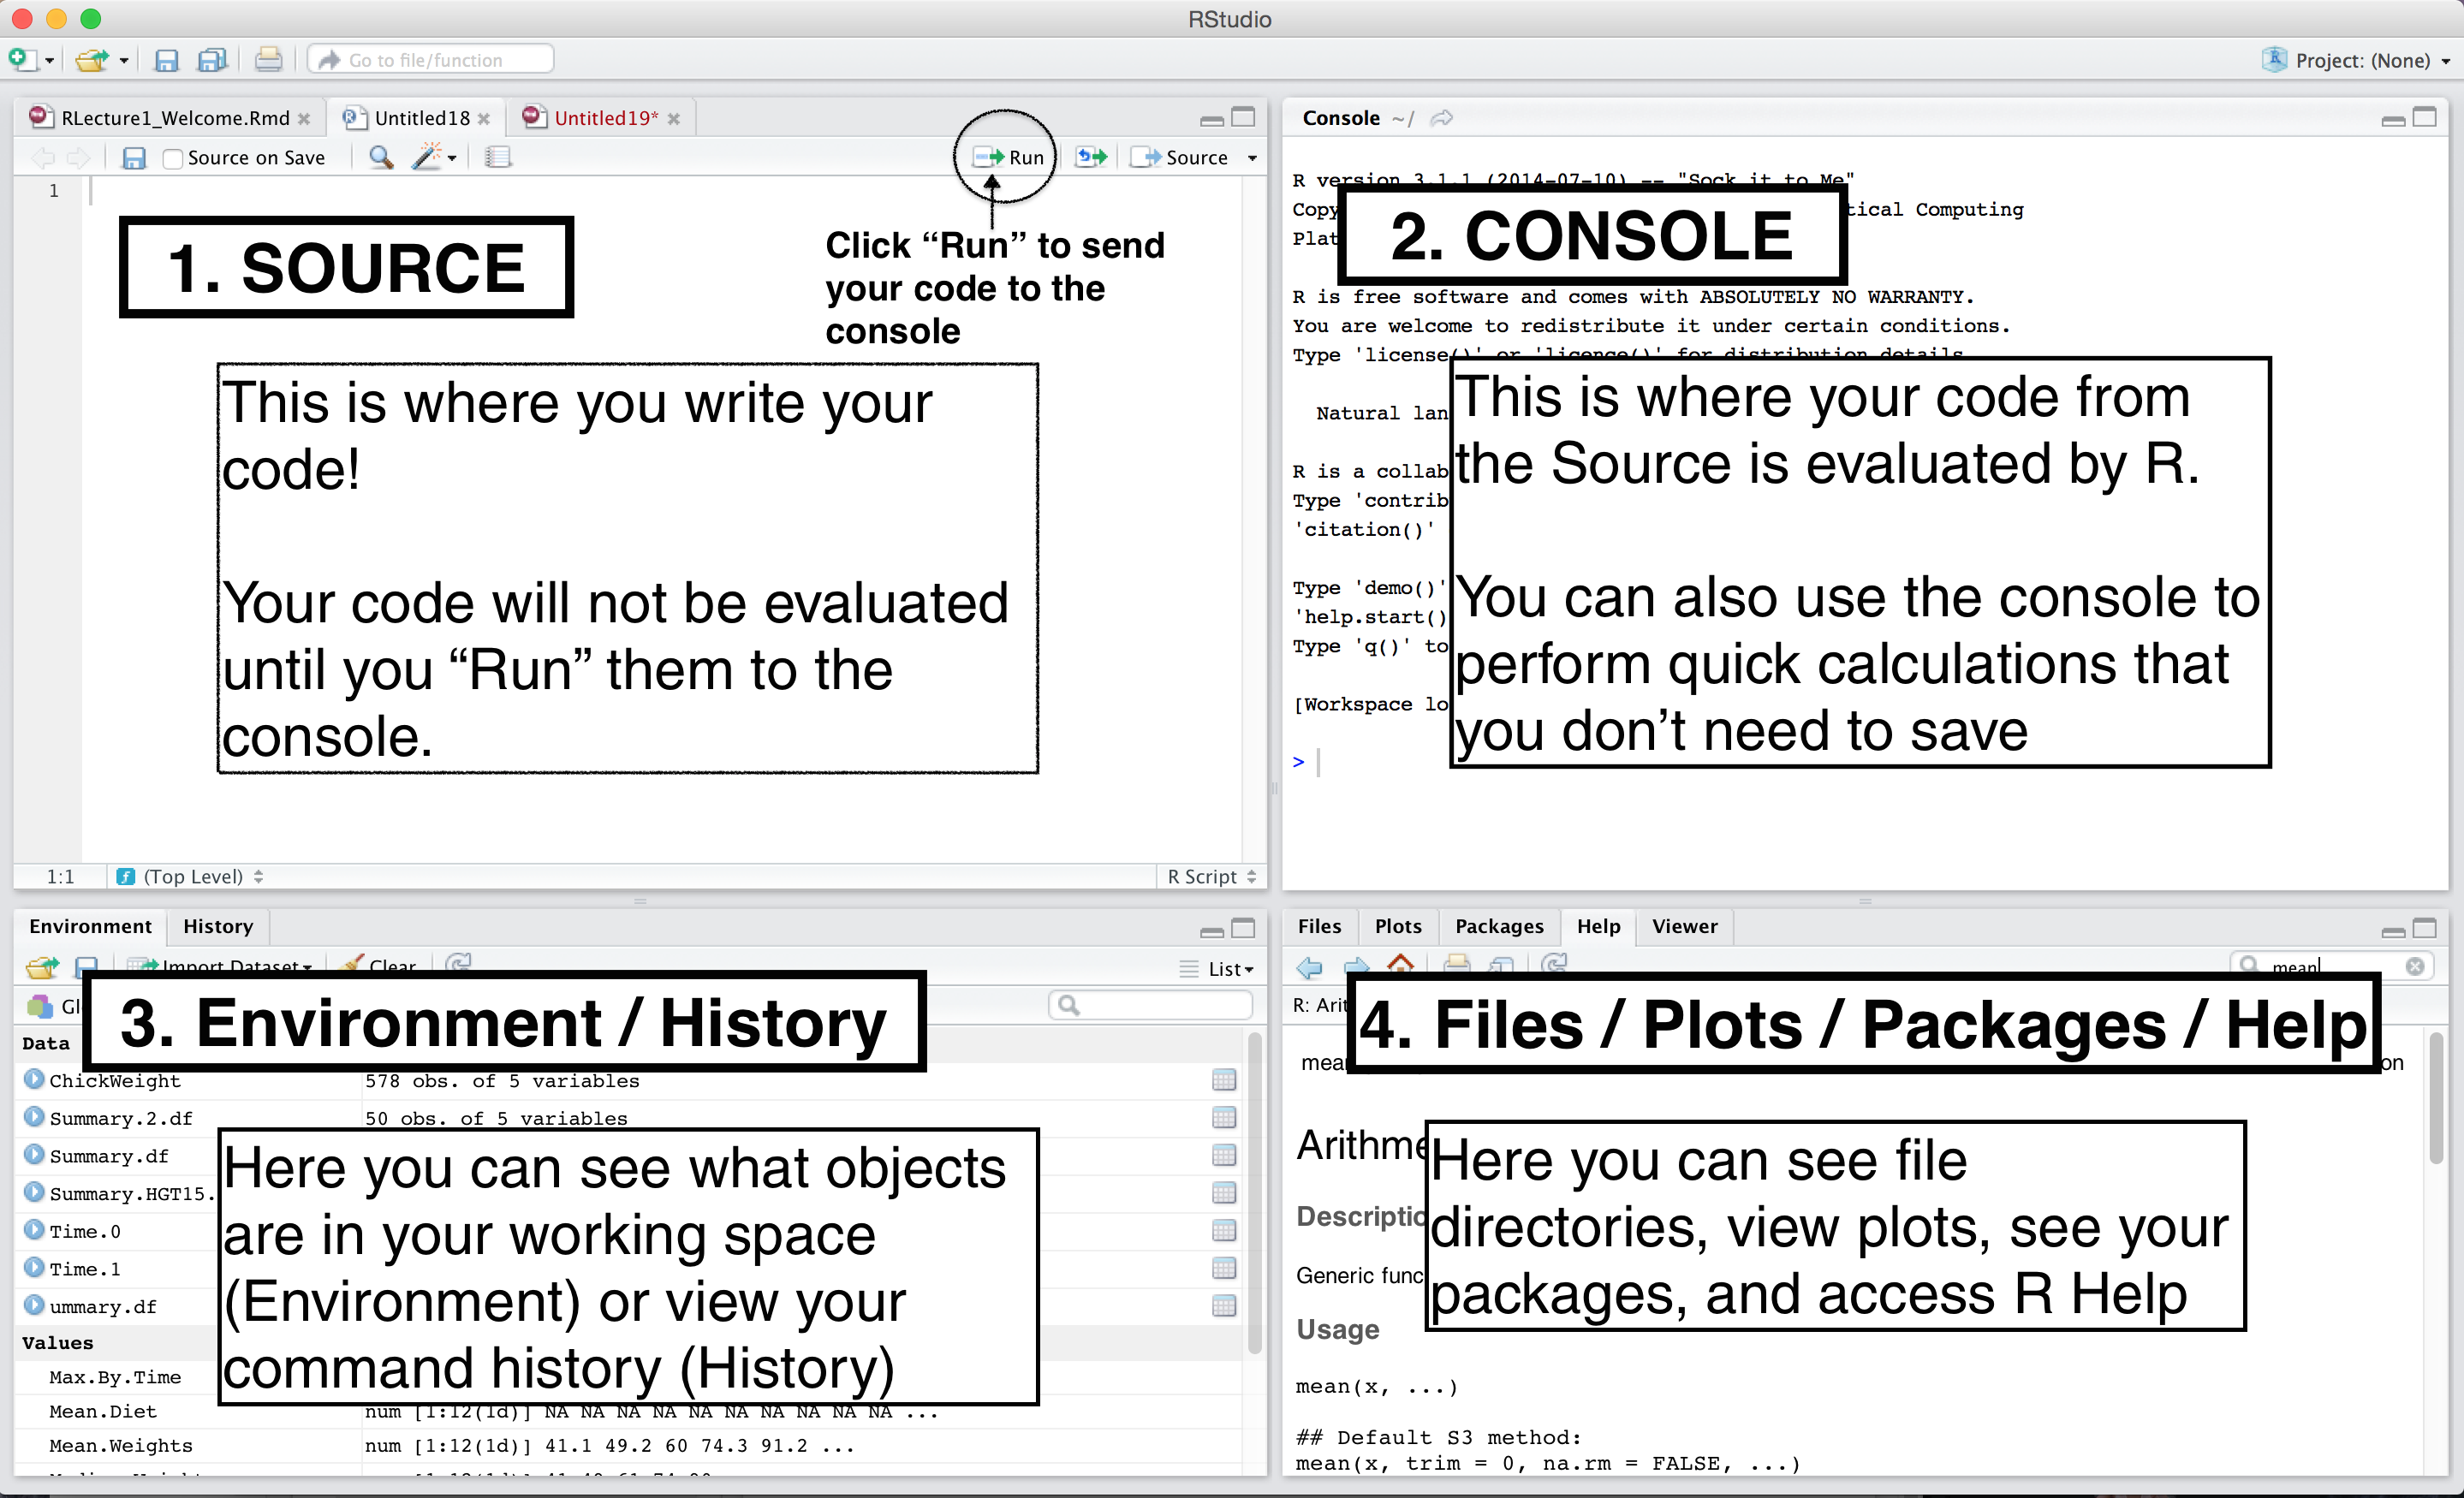
\includegraphics[width=\linewidth]{/Users/Nathaniel/Dropbox/Git/YaRrr_Book/media/RStudio_Screenshot_Labels.png}
\caption{The four panes of RStudio.}
\label{fig:fullfig}
\end{figure*}

Note your windows might be in a different order. You can change the order of the windows under RStudio preferences.

\subsection{Source - Your notepad for code}

The source pane is where you create and edit R Scripts - which are just text files with the ".R" extension. When you open RStudio, it will automatically start a new Untitled script. You will write 99\% of your R code in a script in the source panel. However, your R code will not be evaluated until you 'send' the code to the Console.

You can send your code from the source to the Console by highlighting the code you wish to evaluate and clicking on the "Run" button on the top right of the Source. Alternatively, you can use the hot-key "Command + Return" on Mac, or "Control + Enter" on PC to send code to the console.



\subsection{Console: The calculator}

The console is where R actually executes (calculates) code. You can type code directly into the console and get an immediate response. For example, if you type 1+1 into the console, you'll see that R immediately gives an output of 2

\begin{footnotesize}
\begin{knitrout}
\definecolor{shadecolor}{rgb}{0.969, 0.969, 0.969}\color{fgcolor}\begin{kframe}
\begin{alltt}
\hlnum{1}\hlopt{+}\hlnum{1}
\end{alltt}
\begin{verbatim}
## [1] 2
\end{verbatim}
\end{kframe}
\end{knitrout}
\end{footnotesize}

\marginnote{Tip: Try to write most of your code in a document in the Source. Only type directly into the Console to de-bug or do quick analyses.}

However, most of the time, you won't be typing directly into the console. Instead, you'll be writing code in the source and then "Running" it to the console. The reason for this is straightforward: If you type code into the console, it won't be saved (though you can look back on your command History). And if you make a mistake in typing code into the console, you'd have to re-type everything all over again. Instead, it's better to write all your code in the Source. When you are ready to execute some code, you can then send "Run" it to the console.

\subsection{Environment / History}

The Environment tab of this panel shows you the names of all the data objects (like vectors, matrices, and dataframes) that you've defined in your current R session. The tab also has a few clickable actions like importing a new dataset. However, I almost never look at this menu.

The History tab of this panel simply shows you a history of your R commands. I never look at this. In fact, I didn't realize it was even there until I started writing this tutorial.

\subsection{Files / Plots / Packages / Help}

This panel shows you file directories, plots, your current packages, and help menus.

\begin{enumerate}
\item Files - Gives you access to the file directory on your harddrive. One nice feature of the "Files" panel is that you can use it to set your working directory - once you navigate to a folder you want to read and save files to, click "More" and then "Set As Working Directory."
\item Plots - Shows your plots. There are buttons for opening the plot in a separate window and exporting the plot as a pdf or jpeg (though you can also do this with code using the \texttt{pdf()} or \texttt{jpeg()} functions.)\marginnote{Most - if not all - of the time when you perform actions using your mouse by pointing and clicking in RStudio, RStudio will perform the function by sending the appropriate R Code to the console. You can then copy and paste this code into your documents to automate the process later.}
\item Packages - Shows a list of all the R packages installed on your harddrive and indicates whether or not they are currently loaded. Packages that are loaded in the current session are checked while those that are installed but not yet loaded are unchecked.
\item Help - Help menu for R functions. You can either type the name of a function in the search window, or use the code \texttt{?function.name} to search for a function with the name \texttt{function.name}
\end{enumerate}


To see how plots are displayed try the following command which should display a histogram of 100 values randomly drawn from a standard normal distribution.

\begin{footnotesize}
\begin{knitrout}
\definecolor{shadecolor}{rgb}{0.969, 0.969, 0.969}\color{fgcolor}\begin{kframe}
\begin{alltt}
\hlkwd{hist}\hlstd{(}\hlkwc{x} \hlstd{=} \hlkwd{rnorm}\hlstd{(}\hlkwc{n} \hlstd{=} \hlnum{100}\hlstd{,} \hlkwc{mean} \hlstd{=} \hlnum{1000}\hlstd{,} \hlkwc{sd} \hlstd{=} \hlnum{100}\hlstd{),}
     \hlkwc{main} \hlstd{=} \hlstr{"Plunder in 2015"}\hlstd{,}
     \hlkwc{xlab} \hlstd{=} \hlstr{"Amount"}
     \hlstd{)}
\end{alltt}
\end{kframe}
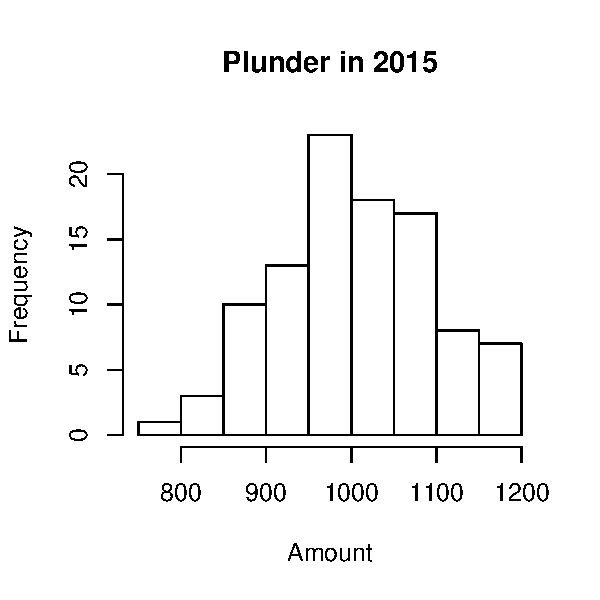
\includegraphics[width=\maxwidth]{figure/unnamed-chunk-4-1} 

\end{knitrout}
\end{footnotesize}

\section{Getting help}

To get help and see documentation for a function, type \texttt{?fun}, where \texttt{fun} is the name of the function. For example, to get additional information on the histogram function, run the following code:

\marginnote{Tip: If you ever need to learn more about an R function: type \texttt{?functionname}, where \texttt{functionname} is the name of the function.}

\begin{footnotesize}
\begin{knitrout}
\definecolor{shadecolor}{rgb}{0.969, 0.969, 0.969}\color{fgcolor}\begin{kframe}
\begin{alltt}
\hlopt{?}\hlstd{hist}
\end{alltt}
\end{kframe}
\end{knitrout}
\end{footnotesize}


\section{Installing and loading packages}

When you download and install R for the first time, you are installing the Base R software. Base R will will contain most if not all the functions you need. However, one of the great things about R is that people are constantly writing and sharing new functions that you can use. When people share a new function, they usually do so in the form of an \textit{R package} which contains anything from functions, to help menus, to vignettes (examples), to data. To install a new R package, you need to run the code \texttt{install.packages("package")}, where "package" is the name of the package. After you've installed the package, you need to \textit{load} it into R by running the code \texttt{load("package)}. This will load the package into your current R session and allow you to use its contents.\marginnote{Once you've installed a package on your computer, you never need to install it again. However, you do need to load the package every time you start a new R session.}

For example, let's say you want to create a wordcloud - a graph that plots text in different sizes. You can certainly program this yourself in R, but thankfully someone has created a package called \texttt{wordcloud} with a function that will do this for you. Let's install the package, load it, and then use the \texttt{wordcloud} function:

\begin{footnotesize}
\begin{knitrout}
\definecolor{shadecolor}{rgb}{0.969, 0.969, 0.969}\color{fgcolor}\begin{kframe}
\begin{alltt}
\hlkwd{install.packages}\hlstd{(}\hlstr{"wordcloud"}\hlstd{)}
\end{alltt}
\begin{verbatim}
## 
## The downloaded binary packages are in
## 	/var/folders/yh/4fyk9h754h7fnmpgyc6p5whw0000gn/T//RtmpJ3VXTu/downloaded_packages
\end{verbatim}
\begin{alltt}
\hlkwd{library}\hlstd{(}\hlstr{"wordcloud"}\hlstd{)} \hlcom{# Install the package}
\end{alltt}


{\ttfamily\noindent\itshape\color{messagecolor}{\#\# Loading required package: RColorBrewer}}\begin{alltt}
\hlkwd{par}\hlstd{(}\hlkwc{mar} \hlstd{=} \hlkwd{rep}\hlstd{(}\hlnum{0}\hlstd{,} \hlnum{4}\hlstd{))}
\hlkwd{wordcloud}\hlstd{(}\hlkwc{words} \hlstd{=} \hlkwd{c}\hlstd{(}\hlstr{"sword"}\hlstd{,} \hlstr{"YaRrr!"}\hlstd{,} \hlstr{"eyepatch"}\hlstd{,}
                    \hlstr{"parrot"}\hlstd{,} \hlstr{"plunder"}\hlstd{,} \hlstr{"treasure"}\hlstd{,}
                    \hlstr{"chest"}\hlstd{,} \hlstr{"scurvy"}\hlstd{),}
          \hlkwc{freq} \hlstd{=} \hlkwd{sample}\hlstd{(}\hlnum{50}\hlopt{:}\hlnum{1000}\hlstd{,} \hlnum{8}\hlstd{),}
          \hlkwc{colors} \hlstd{=} \hlkwd{gray}\hlstd{(}\hlkwd{runif}\hlstd{(}\hlnum{8}\hlstd{,} \hlnum{0}\hlstd{,} \hlnum{1}\hlstd{)))}
\end{alltt}
\end{kframe}
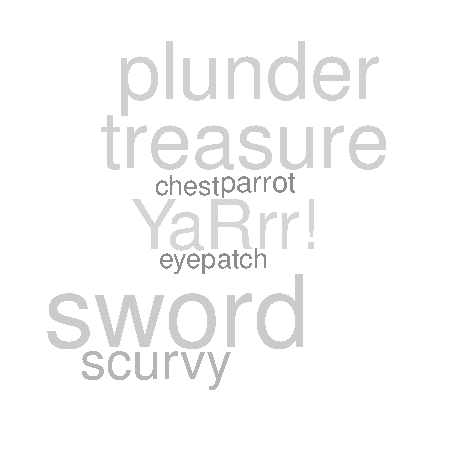
\includegraphics[width=\maxwidth]{figure/unnamed-chunk-6-1} 

\end{knitrout}
\end{footnotesize}



\section{Downloading and loading the pirate dataset}

For much of this book, we will be referring to the \texttt{pirate} dataset. This dataset contains the results of a survey completed by 1,000 pirates that have been on my crew. To download this dataset, execute the following code:

\begin{knitrout}
\definecolor{shadecolor}{rgb}{0.969, 0.969, 0.969}\color{fgcolor}\begin{kframe}
\begin{alltt}
\hlstd{pirates} \hlkwb{<-} \hlkwd{read.table}\hlstd{(}\hlkwc{file} \hlstd{=} \hlstr{"http://nathanieldphillips.com/wp-content/uploads/2015/05/pirate_survey.txt"}\hlstd{,}
           \hlkwc{header} \hlstd{= T,}
           \hlkwc{sep} \hlstd{=} \hlstr{"\textbackslash{}t"}\hlstd{,}
           \hlkwc{stringsAsFactors} \hlstd{= F}
           \hlstd{)}
\end{alltt}
\end{kframe}
\end{knitrout}

If you'd like to see how the dataset looks, you can execute the \texttt{View()} function:

\begin{knitrout}
\definecolor{shadecolor}{rgb}{0.969, 0.969, 0.969}\color{fgcolor}\begin{kframe}
\begin{alltt}
\hlkwd{View}\hlstd{(pirates)}
\end{alltt}
\end{kframe}
\end{knitrout}

When you run this command, you should see the first several rows and columns of the dataset (like this:)

\begin{figure*}
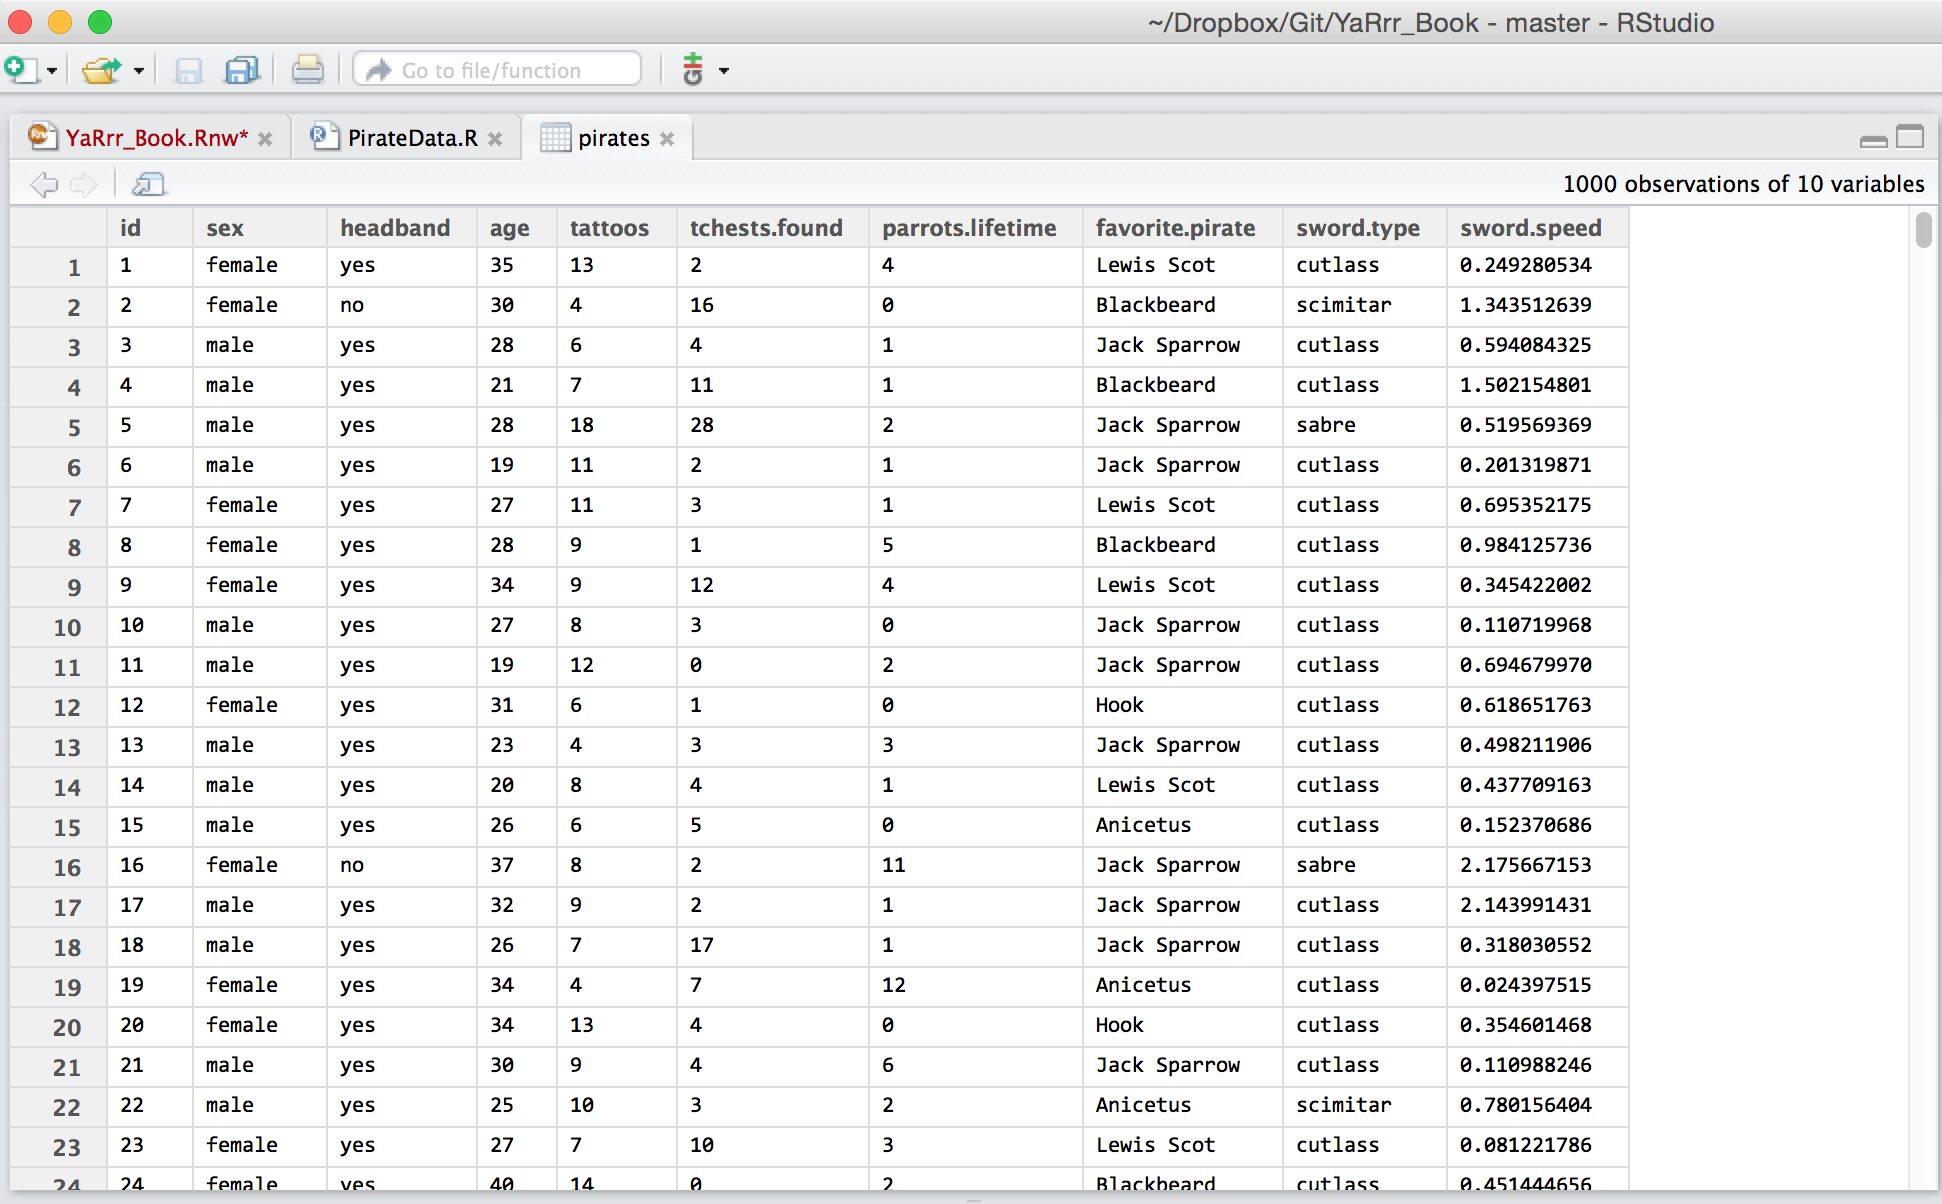
\includegraphics[width=\linewidth]{/Users/Nathaniel/Dropbox/Git/YaRrr_Book/media/pirates_data_screenshot.png}
\caption{The pirates dataset.}
\label{fig:piratesdata}
\end{figure*}



\section{The R Reference Card}

Over the course of this book, you will be learning \textit{lots} of new functions. Wouldn't it be nice if someone created a Cheatsheet / Notecard of many common R functions? Yes it would, and thankfully Tom Short has done this in his creation of the R Reference Card. You can download a copy at <https://dl.dropboxusercontent.com/u/7618380/RReferenceCard.pdf>. I highly encourage you to print this out and start highlighting functions as you learn them!


\subsection{Finished!}

That's it for this lecture! All you did was install the most powerful statistical package on the planet used by top universities and companies like Google. No big deal.

%----------------------------------------------------------------------------------------
%	CHAPTER 2
%----------------------------------------------------------------------------------------

\chapter{2: Coding Basics}
\label{ch:2}


\subsection{Chapter Goals}

\begin{enumerate}
  \item Accept that learning R will take time (and promise you'll never go back to SPSS!)
  \item Know how to use comments and spaces in R code.
  \item Be able to define and manipulate scalars and vectors
  \item Generate vectors using c(), :, rep(), and seq()
\end{enumerate}


\subsection{Before we get started, a word of warning...}

So by now you've installed R and you're ready to get started. But first, let me give you a brief word of warning: Especially if this is your first experience programming, you are going to experience a \textit{lot} of headaches when you get started. You will run into error after error and pound your fists against the table screaming: "WHY ISN'T MY CODE WORKING?!?!? There must be something wrong with this stupid software!!!" You will spend hours trying to find a bug in your code, only to find that - frustratingly enough, you had had an extra space or missed a comma somewhere. You'll then wonder why you ever decided to learn R when (::sigh::) SPSS was so "nice and easy."


\marginnote{Fun fact: SPSS stands for "Shitty Piece of Shitty Shit". True story.}

This is perfectly normal! Don't get discouraged and DON'T GO BACK TO SPSS! Trust me, as you gain more programming experience, you'll experience fewer and fewer bugs (though they'll never go away completely). Once you get over the initial barriers, you'll find yourself conducting analyses much, much faster than you ever did before.

\subsection{The basics of R programming}

Ok, let's write some code! Again, we will write all our code in a script file in the Source pane of RStudio. When we want to execute it, we'll send it to the Console.

\subsection{R as a calculator}

At its heart, R is just a fancy calculator. Let's do some basic algebra, type the following command into the source, then highlight the text and click "Run" to execute it in the console:

\marginnote{Tip: To execute code from the source to the console, highlight it and use the hot-keys "Command-Return" on Mac or "Control-Enter" on PC.}


\begin{knitrout}
\definecolor{shadecolor}{rgb}{0.969, 0.969, 0.969}\color{fgcolor}\begin{kframe}
\begin{alltt}
\hlnum{1}\hlopt{+}\hlnum{1} \hlcom{# The result should be 2}
\end{alltt}
\begin{verbatim}
## [1] 2
\end{verbatim}
\end{kframe}
\end{knitrout}


As you can see, R returns the (thankfully correct) value of 2. You'll notice that the console also returns the text [1]. This is just telling you you the index of the value next to it. Don't worry about this for now, it will make more sense later.

Additionally, you'll notice that I included a comment in the code using the \# sign. R will ignore everything on a line after the \# sign. So why do we use comments? Mainly to explain to others, including your future self, what you are trying to do with your code.\marginnote{Do your future self a favor and use comments to explain what you're doing with your code. Also, maybe go for a run once in a while.}

Let's try some more simple calculations


\begin{knitrout}
\definecolor{shadecolor}{rgb}{0.969, 0.969, 0.969}\color{fgcolor}\begin{kframe}
\begin{alltt}
\hlnum{2} \hlopt{*} \hlnum{3} \hlopt{-} \hlnum{1} \hlcom{# R ignores spaces}
\end{alltt}
\begin{verbatim}
## [1] 5
\end{verbatim}
\begin{alltt}
\hlnum{2} \hlopt{*} \hlstd{(}\hlnum{3} \hlopt{-} \hlnum{1}\hlstd{)} \hlcom{# R observes order of operations}
\end{alltt}
\begin{verbatim}
## [1] 4
\end{verbatim}
\end{kframe}
\end{knitrout}


As you can see, R ignores spaces in between arguments in code. I recommend using spaces to make your code easier to look at. Personally, I include spaces between arithmetic operators (like + and -) and after commas (which we'll get to later).

\section{Defining objects with the <- assignment}

\marginnote{Good object names strike a balance between being easy to type (i.e.; short names) and interpret. If you have several datasets, it's probably not a good idea to name them \texttt{a}, \texttt{b}, \texttt{c} because you'll forget which is which. However, using long names like \texttt{March2015Group1OnlyFemales} and \texttt{March2015Group1OnlyMales} will give you carpel tunnel syndrome.}

So far so good, you can use R as a simple calculator. Now, let's do our first \textit{object assignment}. Object assignment is our way of storing information, such as a number or a statistical test, into something we can easily refer to later. Let's start by creating the object "mateys" and assigning the outcome of $5*10}$ to it:


\begin{knitrout}
\definecolor{shadecolor}{rgb}{0.969, 0.969, 0.969}\color{fgcolor}\begin{kframe}
\begin{alltt}
\hlcom{# The symbol(s) "<-" mean "assign"}
\hlstd{mateys} \hlkwb{<-} \hlnum{5} \hlopt{*} \hlnum{10} \hlcom{# Assign the value of 5*10 to a new objected called mateys}
\end{alltt}
\end{kframe}
\end{knitrout}

Now, anytime we want to refer to the content of the object \texttt{mateys}, we can just type it. When you assign a value to an object, R won't automatically print it. If you want to see the value, you need to call the object by just executing its name:


\begin{knitrout}
\definecolor{shadecolor}{rgb}{0.969, 0.969, 0.969}\color{fgcolor}\begin{kframe}
\begin{alltt}
\hlstd{mateys} \hlcom{# What is the value of mateys?}
\end{alltt}
\begin{verbatim}
## [1] 50
\end{verbatim}
\end{kframe}
\end{knitrout}


A few notes about defining objects: you can't start the name of an object with a number, and you can't have spaces or other 'weird' characters in the name. Here are some examples of \textit{invalid} object names:


\begin{knitrout}
\definecolor{shadecolor}{rgb}{0.969, 0.969, 0.969}\color{fgcolor}\begin{kframe}
\begin{alltt}
me mateys <- 50 \hlcom{# Can't have spaces}
5.mateys <- 50 \hlcom{# Can't start a name with a number}
mayeys! <- 5 0# Can't have an \hlstr{"!"} in the object name
\end{alltt}
\end{kframe}
\end{knitrout}


R is case-sensitive. If you define an object with uppercase letters, you must keep referring to it with uppercase letters!

\marginnote{Avoid using too many capital letters in object names because they require you to hold the shift key. This may sound silly, but you'd be surprised how much easier it is to type \texttt{mydata} than \texttt{MyData} 100 times.}


\begin{knitrout}
\definecolor{shadecolor}{rgb}{0.969, 0.969, 0.969}\color{fgcolor}\begin{kframe}
\begin{alltt}
\hlstd{Plunder} \hlkwb{<-} \hlnum{1}
\hlstd{plunder} \hlkwb{<-} \hlnum{100}
\hlstd{Plunder}
\end{alltt}
\begin{verbatim}
## [1] 1
\end{verbatim}
\begin{alltt}
\hlstd{plunder}
\end{alltt}
\begin{verbatim}
## [1] 100
\end{verbatim}
\end{kframe}
\end{knitrout}


Once you've defined an object, you can use it in other commands:

\begin{knitrout}
\definecolor{shadecolor}{rgb}{0.969, 0.969, 0.969}\color{fgcolor}\begin{kframe}
\begin{alltt}
\hlstd{a} \hlkwb{<-} \hlnum{100}
\hlstd{b} \hlkwb{<-} \hlnum{2}
\hlstd{c} \hlkwb{<-} \hlstd{a} \hlopt{+} \hlstd{b}
\hlstd{c}
\end{alltt}
\begin{verbatim}
## [1] 102
\end{verbatim}
\end{kframe}
\end{knitrout}


If you want to change an object, you can just reassign it. You can even refer to the same object when reassigning it:


\begin{knitrout}
\definecolor{shadecolor}{rgb}{0.969, 0.969, 0.969}\color{fgcolor}\begin{kframe}
\begin{alltt}
\hlstd{a} \hlkwb{<-} \hlnum{2}
\hlstd{a} \hlkwb{<-} \hlstd{a} \hlopt{+} \hlstd{a}
\hlstd{a}
\end{alltt}
\begin{verbatim}
## [1] 4
\end{verbatim}
\end{kframe}
\end{knitrout}


\marginnote{You can use \texttt{=} instead of \texttt{<-} for object assignment but I recommend you stick with \textt{<-} because the direction of the assignment is clear.}


\section{Data object types in R}

R stores everything as an object, and there are different types of objects. The first two objects we'll learn about are scalars and vectors. Later on, we'll talk about more complicated objects like matrices, dataframes, hypothesis tests, etc.

\subsection{Two simple data objects: scalars and vectors}

Two of the most common data objects in R are \textbf{scalars} and \textbf{vectors}. Let's discuss each in turn,

\subsection{scalars}

A \textbf{scalar} is just a single value. A scalar can either be \textit{numeric} or \textit{string}. A numeric scalar is a number, while a string scalar is a letter. We denote string scalars by using quotation marks. Here are some examples:

\begin{knitrout}
\definecolor{shadecolor}{rgb}{0.969, 0.969, 0.969}\color{fgcolor}\begin{kframe}
\begin{alltt}
\hlstd{a} \hlkwb{<-} \hlnum{1}
\hlstd{b} \hlkwb{<-} \hlnum{3} \hlopt{*} \hlnum{40}
\hlstd{ship} \hlkwb{<-} \hlstr{"Black Pearl"}
\end{alltt}
\end{kframe}
\end{knitrout}



\begin{marginfigure}
\begin{tiny}
\begin{knitrout}
\definecolor{shadecolor}{rgb}{0.969, 0.969, 0.969}\color{fgcolor}\begin{kframe}
\begin{alltt}
\hlcom{# scalar v vector v matrix  }

\hlkwd{par}\hlstd{(}\hlkwc{mar} \hlstd{=} \hlkwd{rep}\hlstd{(}\hlnum{1}\hlstd{,} \hlnum{4}\hlstd{))}
\hlkwd{plot}\hlstd{(}\hlnum{1}\hlstd{,} \hlkwc{xlim} \hlstd{=} \hlkwd{c}\hlstd{(}\hlnum{0}\hlstd{,} \hlnum{4}\hlstd{),} \hlkwc{ylim} \hlstd{=} \hlkwd{c}\hlstd{(}\hlopt{-}\hlnum{.5}\hlstd{,} \hlnum{5}\hlstd{),}
     \hlkwc{xlab} \hlstd{=} \hlstr{""}\hlstd{,} \hlkwc{ylab} \hlstd{=} \hlstr{""}\hlstd{,}
     \hlkwc{xaxt} \hlstd{=} \hlstr{"n"}\hlstd{,} \hlkwc{yaxt} \hlstd{=} \hlstr{"n"}\hlstd{,}
     \hlkwc{bty} \hlstd{=} \hlstr{"n"}\hlstd{,} \hlkwc{type} \hlstd{=} \hlstr{"n"}\hlstd{)}

\hlcom{# scalar}
\hlkwd{rect}\hlstd{(}\hlkwd{rep}\hlstd{(}\hlnum{0}\hlstd{,} \hlnum{1}\hlstd{),} \hlkwd{rep}\hlstd{(}\hlnum{0}\hlstd{,} \hlnum{1}\hlstd{),} \hlkwd{rep}\hlstd{(}\hlnum{1}\hlstd{,} \hlnum{1}\hlstd{),} \hlkwd{rep}\hlstd{(}\hlnum{1}\hlstd{,} \hlnum{1}\hlstd{))}
\hlkwd{text}\hlstd{(}\hlnum{.5}\hlstd{,} \hlopt{-}\hlnum{.5}\hlstd{,} \hlstr{"scalar"}\hlstd{)}

\hlcom{# Vector}
\hlkwd{rect}\hlstd{(}\hlkwd{rep}\hlstd{(}\hlnum{2}\hlstd{,} \hlnum{5}\hlstd{),} \hlnum{0}\hlopt{:}\hlnum{4}\hlstd{,} \hlkwd{rep}\hlstd{(}\hlnum{3}\hlstd{,} \hlnum{5}\hlstd{),} \hlnum{1}\hlopt{:}\hlnum{5}\hlstd{)}
\hlkwd{text}\hlstd{(}\hlnum{2.5}\hlstd{,} \hlopt{-}\hlnum{.5}\hlstd{,} \hlstr{"Vector"}\hlstd{)}
\end{alltt}
\end{kframe}
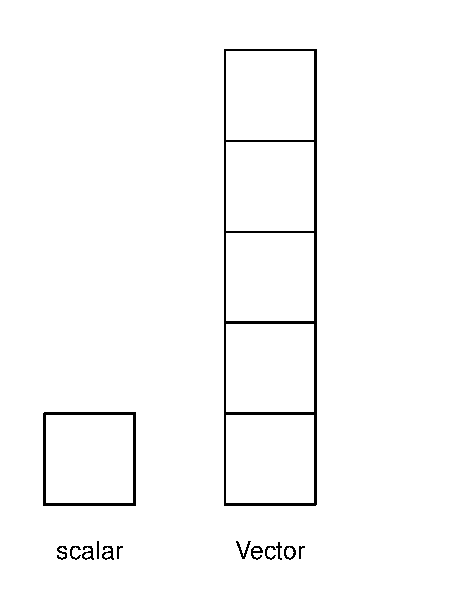
\includegraphics[width=\maxwidth]{figure/unnamed-chunk-18-1} 

\end{knitrout}
\caption{Visual depiction of a scalar and vector. Deep shit. Wait until we get to matrices - you're going to lose it.}
\label{fig:scalarvector}
\end{tiny}
\end{marginfigure}

It is important to note that once you've defined an object, you refer to it without quotation marks, even if the object is a character. For example, to refer to the object \texttt{ship} that I defined above, you need to write \texttt{ship} without quotations marks


\begin{knitrout}
\definecolor{shadecolor}{rgb}{0.969, 0.969, 0.969}\color{fgcolor}\begin{kframe}
\begin{alltt}
\hlstd{ship} \hlcom{# Print the value of the object ship}
\end{alltt}
\begin{verbatim}
## [1] "Black Pearl"
\end{verbatim}
\begin{alltt}
\hlstr{"ship"} \hlcom{# R thinks this is a new string called "ship", not the object called ship}
\end{alltt}
\begin{verbatim}
## [1] "ship"
\end{verbatim}
\end{kframe}
\end{knitrout}


\subsection{Vectors}

A \textbf{vector} is a combination of several scalars. For example, the numbers from one to ten could be a vector of length 10. Like scalars, you can also create character vectors that contain character scalars.


There are many ways to create vectors in R, here are the most common:

\vspace{5mm} %5mm vertical space
\noindent
\setlength{\fboxrule}{1.5pt}
\fbox{
\parbox{\textwidth}{

\newfun{c(a, b, c, ...)}\index{c()}

\hline

\begin{description}

  \item[\tt{a, b, c, ...}] \hfill \\
      One or more objects to be combined into a vector
\end{description}

}
}
\vspace{5mm} %5mm vertical space


The simplest way to create a vector is with the \texttt{c()} function. The c here stands for concatenate, which means "bring them together". When using c(), place a comma in between the objects (scalers or vectors) you want to combine:

\marginnote{\texttt{c(x, y, z)}: Create a vector with the c() command by separating elements with commas}

The following code will create a vector of the integers from 1 to 5:

\begin{knitrout}
\definecolor{shadecolor}{rgb}{0.969, 0.969, 0.969}\color{fgcolor}\begin{kframe}
\begin{alltt}
\hlstd{v} \hlkwb{<-} \hlkwd{c}\hlstd{(}\hlnum{1}\hlstd{,} \hlnum{2}\hlstd{,} \hlnum{3}\hlstd{,} \hlnum{4}\hlstd{,} \hlnum{5}\hlstd{)}
\hlstd{v}
\end{alltt}
\begin{verbatim}
## [1] 1 2 3 4 5
\end{verbatim}
\end{kframe}
\end{knitrout}

You can also create vectors by combining objects you have already defined. Let's create a vector of the numbers from 1 to 10 by first generating a vector \texttt{a} from 1 to 5, and a vector \texttt{b} from 6 to 10 then combine them into a single vector \texttt{c}:

\begin{knitrout}
\definecolor{shadecolor}{rgb}{0.969, 0.969, 0.969}\color{fgcolor}\begin{kframe}
\begin{alltt}
\hlstd{a} \hlkwb{<-} \hlkwd{c}\hlstd{(}\hlnum{1}\hlstd{,} \hlnum{2}\hlstd{,} \hlnum{3}\hlstd{,} \hlnum{4}\hlstd{,} \hlnum{5}\hlstd{)}
\hlstd{b} \hlkwb{<-} \hlkwd{c}\hlstd{(}\hlnum{6}\hlstd{,} \hlnum{7}\hlstd{,} \hlnum{8}\hlstd{,} \hlnum{9}\hlstd{,} \hlnum{10}\hlstd{)}
\hlstd{c} \hlkwb{<-} \hlkwd{c}\hlstd{(a, b)}
\hlstd{c}
\end{alltt}
\begin{verbatim}
##  [1]  1  2  3  4  5  6  7  8  9 10
\end{verbatim}
\end{kframe}
\end{knitrout}

You can also create string vectors containing only string values:

\begin{knitrout}
\definecolor{shadecolor}{rgb}{0.969, 0.969, 0.969}\color{fgcolor}\begin{kframe}
\begin{alltt}
\hlstd{a} \hlkwb{<-} \hlkwd{c}\hlstd{(}\hlstr{"this"}\hlstd{,} \hlstr{"is"}\hlstd{,} \hlstr{"a"}\hlstd{,} \hlstr{"string"}\hlstd{,} \hlstr{"vector"}\hlstd{)}
\hlstd{a}
\end{alltt}
\begin{verbatim}
## [1] "this"   "is"     "a"      "string" "vector"
\end{verbatim}
\end{kframe}
\end{knitrout}



A vector can only contain one type of scalar: either numeric or character. If you try to create a vector with numeric and character scalars, then R will convert all of the numeric scalars to characters:


\begin{knitrout}
\definecolor{shadecolor}{rgb}{0.969, 0.969, 0.969}\color{fgcolor}\begin{kframe}
\begin{alltt}
\hlstd{movie} \hlkwb{<-} \hlstr{"Pirates of the Carribean"}
\hlstd{revenue} \hlkwb{<-} \hlnum{634954111}
\hlkwd{c}\hlstd{(movie, revenue)} \hlcom{# Result is a string vector}
\end{alltt}
\begin{verbatim}
## [1] "Pirates of the Carribean" "634954111"
\end{verbatim}
\end{kframe}
\end{knitrout}


Once you've created a vector, you can easily determine its length by using the \texttt{length()} function:

\newfun{length()}\index{length()}

\begin{knitrout}
\definecolor{shadecolor}{rgb}{0.969, 0.969, 0.969}\color{fgcolor}\begin{kframe}
\begin{alltt}
\hlkwd{length}\hlstd{(}\hlkwd{c}\hlstd{(}\hlnum{1}\hlstd{,} \hlnum{2}\hlstd{,} \hlnum{3}\hlstd{))}
\end{alltt}
\begin{verbatim}
## [1] 3
\end{verbatim}
\end{kframe}
\end{knitrout}


\section{Generating numeric vectors}

While the c() operator is the most straightforward way to create a vector, it's also one of the most tedious. Let's say you wanted to create a vector of all integers from 1 to 100. You definitely don't want to have to type all the numbers into a c() operator. Instead, R has many simple built-in functions for generating numeric vectors. Let's start with three of them:

\vspace{5mm} %5mm vertical space
\noindent
\setlength{\fboxrule}{1.5pt}
\fbox{
\parbox{\textwidth}{

\newfun{a:b}\index{a:b}

\hline

\begin{description}

  \item[\tt{a}] \hfill \\
      The start of the sequence
  \item[\tt{b}] \hfill \\
      The end of the sequence
\end{description}

}
}
\vspace{5mm} %5mm vertical space

The \texttt{a:b} function creates a vector of numbers from the starting point a to the ending point b in steps of 1:

\begin{footnotesize}
\begin{knitrout}
\definecolor{shadecolor}{rgb}{0.969, 0.969, 0.969}\color{fgcolor}\begin{kframe}
\begin{alltt}
\hlnum{1} \hlopt{:} \hlnum{10} \hlcom{# Integers from 1 to 10}
\end{alltt}
\begin{verbatim}
##  [1]  1  2  3  4  5  6  7  8  9 10
\end{verbatim}
\begin{alltt}
\hlnum{10} \hlopt{:} \hlnum{1} \hlcom{# Integers from 10 to 1}
\end{alltt}
\begin{verbatim}
##  [1] 10  9  8  7  6  5  4  3  2  1
\end{verbatim}
\begin{alltt}
\hlnum{20.1}\hlopt{:}\hlnum{30.1} \hlcom{# From 20.1 to 30.1}
\end{alltt}
\begin{verbatim}
##  [1] 20.1 21.1 22.1 23.1 24.1 25.1 26.1 27.1 28.1 29.1 30.1
\end{verbatim}
\end{kframe}
\end{knitrout}
\end{footnotesize}



\vspace{5mm} %5mm vertical space
\noindent
\setlength{\fboxrule}{1.5pt}
\fbox{
\parbox{\textwidth}{

\newfun{seq(from, to, by)}\index{seq()}

\hline

\begin{description}

  \item[\tt{from}] \hfill \\
      The start of the sequence
  \item[\tt{to}] \hfill \\
      The end of the sequence
  \item[\tt{by}] \hfill \\
      The step-size of the sequence \\
  \item[\tt{length.out}] \hfill \\
      The desired length of the final sequence (only use if you don't specify \texttt{by})
\end{description}

}
}
\vspace{5mm} %5mm vertical space

\marginnote{\textbf{seq(from, to, by)} - Creates a sequence between two numbers in steps that you specify. \\ \texttt{from}: The starting value \\ \texttt{to}: The ending value \\ \texttt{by}: The step size between \texttt{begin} and \texttt{end}}

The \texttt{seq()} function allows you to create a sequence from a starting number to an ending number, in steps you specify. The function has three arguments, which are inputs to the function which changes how it works.

\begin{footnotesize}
\begin{knitrout}
\definecolor{shadecolor}{rgb}{0.969, 0.969, 0.969}\color{fgcolor}\begin{kframe}
\begin{alltt}
\hlkwd{seq}\hlstd{(}\hlkwc{from} \hlstd{=} \hlnum{1}\hlstd{,} \hlkwc{to} \hlstd{=} \hlnum{10}\hlstd{,} \hlkwc{by} \hlstd{=} \hlnum{1}\hlstd{)}
\end{alltt}
\begin{verbatim}
##  [1]  1  2  3  4  5  6  7  8  9 10
\end{verbatim}
\begin{alltt}
\hlkwd{seq}\hlstd{(}\hlkwc{from} \hlstd{=} \hlnum{0}\hlstd{,} \hlkwc{to} \hlstd{=} \hlnum{100}\hlstd{,} \hlkwc{by} \hlstd{=} \hlnum{10}\hlstd{)}
\end{alltt}
\begin{verbatim}
##  [1]   0  10  20  30  40  50  60  70  80  90 100
\end{verbatim}
\end{kframe}
\end{knitrout}
\end{footnotesize}


The \texttt{rep()} function rep allows you to repeat a number (or vector) a specified number of times. There are three arguments to the rep function:

\vspace{5mm} %5mm vertical space
\noindent
\setlength{\fboxrule}{1.5pt}
\fbox{
\parbox{\textwidth}{

\newfun{rep(x, times, each)}\index{rep()}

\hline

\begin{description}

  \item[\tt{x}] \hfill \\
      A scaler or vector of values to repeat
  \item[\tt{times}] \hfill \\
      The number of times to repeat the sequence
  \item[\tt{each}] \hfill \\
      The number of times to repeat each value within the sequence \\
\end{description}

}
}
\vspace{5mm} %5mm vertical space

\marginnote{\textbf{rep(x, times, each)} - Repeats the numbers in x in a manner you specify \\ \texttt{times}: The number of times the vector should be repeated \\ \texttt{each}: The number of times you want to repeat each element in the vector.}


\begin{footnotesize}
\begin{knitrout}
\definecolor{shadecolor}{rgb}{0.969, 0.969, 0.969}\color{fgcolor}\begin{kframe}
\begin{alltt}
\hlkwd{rep}\hlstd{(}\hlnum{1}\hlopt{:}\hlnum{5}\hlstd{,} \hlkwc{times} \hlstd{=} \hlnum{2}\hlstd{)} \hlcom{# Repeat integers 1 to 5 two times}
\end{alltt}
\begin{verbatim}
##  [1] 1 2 3 4 5 1 2 3 4 5
\end{verbatim}
\begin{alltt}
\hlkwd{rep}\hlstd{(}\hlnum{1}\hlopt{:}\hlnum{5}\hlstd{,} \hlkwc{each} \hlstd{=} \hlnum{2}\hlstd{)} \hlcom{# Repeat each integer from 1 to 5 two times}
\end{alltt}
\begin{verbatim}
##  [1] 1 1 2 2 3 3 4 4 5 5
\end{verbatim}
\begin{alltt}
\hlkwd{rep}\hlstd{(}\hlnum{1}\hlopt{:}\hlnum{5}\hlstd{,} \hlkwc{each} \hlstd{=} \hlnum{2}\hlstd{,} \hlkwc{times} \hlstd{=} \hlnum{2}\hlstd{)} \hlcom{# Do both!}
\end{alltt}
\begin{verbatim}
##  [1] 1 1 2 2 3 3 4 4 5 5 1 1 2 2 3 3 4 4 5 5
\end{verbatim}
\end{kframe}
\end{knitrout}
\end{footnotesize}

\subsection{Arithmetic operations on scalars and vectors}

You can do basic arithmetic operations like +, -, * and / on scalars and vectors. If you do an operation on a vector with a scalar, R will apply the scalar to each element in the vector:

\begin{footnotesize}
\begin{knitrout}
\definecolor{shadecolor}{rgb}{0.969, 0.969, 0.969}\color{fgcolor}\begin{kframe}
\begin{alltt}
\hlstd{a} \hlkwb{<-} \hlnum{1}\hlopt{:}\hlnum{5}
\hlstd{a} \hlopt{*} \hlnum{10}
\end{alltt}
\begin{verbatim}
## [1] 10 20 30 40 50
\end{verbatim}
\begin{alltt}
\hlstd{a} \hlopt{-} \hlnum{1}
\end{alltt}
\begin{verbatim}
## [1] 0 1 2 3 4
\end{verbatim}
\begin{alltt}
\hlstd{a} \hlopt{^} \hlnum{2}
\end{alltt}
\begin{verbatim}
## [1]  1  4  9 16 25
\end{verbatim}
\end{kframe}
\end{knitrout}
\end{footnotesize}

If you do an operation on two vectors, R will try to apply the operation between the vectors by each item:

\begin{footnotesize}
\begin{knitrout}
\definecolor{shadecolor}{rgb}{0.969, 0.969, 0.969}\color{fgcolor}\begin{kframe}
\begin{alltt}
\hlnum{1}\hlopt{:}\hlnum{10} \hlopt{+} \hlnum{21}\hlopt{:}\hlnum{30}
\end{alltt}
\begin{verbatim}
##  [1] 22 24 26 28 30 32 34 36 38 40
\end{verbatim}
\begin{alltt}
\hlstd{(}\hlnum{1}\hlopt{:}\hlnum{5}\hlstd{)} \hlopt{*} \hlstd{(}\hlnum{1}\hlopt{:}\hlnum{5}\hlstd{)}
\end{alltt}
\begin{verbatim}
## [1]  1  4  9 16 25
\end{verbatim}
\begin{alltt}
\hlkwd{seq}\hlstd{(}\hlnum{10}\hlstd{,} \hlnum{100}\hlstd{,} \hlnum{10}\hlstd{)} \hlopt{+} \hlnum{1}\hlopt{:}\hlnum{10}
\end{alltt}
\begin{verbatim}
##  [1]  11  22  33  44  55  66  77  88  99 110
\end{verbatim}
\end{kframe}
\end{knitrout}
\end{footnotesize}

\subsection{Additional Tips}


\begin{enumerate}
  \item To get more tips on how good coding techniques, check out the R style guide at http://adv-r.had.co.nz/Style.html
  \item For great blog articles on R, check out http://www.r-bloggers.com/
  \item If you need to enter a lot of numeric data into R by hand you might want to use the \texttt{scan()} function. This function allows you to easily enter data using 10-key typing on a number pad. To do this, run the code \texttt{scan()} and then enter the data number by number. When you are finished, R will then print the appropriate code to store the data into a vector.
  \item You can run several lines of code in one line by separating the code with the ; key. For example, the following two chunks of code are the same:
  
\begin{knitrout}
\definecolor{shadecolor}{rgb}{0.969, 0.969, 0.969}\color{fgcolor}\begin{kframe}
\begin{alltt}
\hlstd{a} \hlkwb{<-} \hlnum{1}
\hlstd{b} \hlkwb{<-} \hlnum{14}
\hlstd{c} \hlkwb{<-} \hlnum{67}
\end{alltt}
\end{kframe}
\end{knitrout}

\begin{knitrout}
\definecolor{shadecolor}{rgb}{0.969, 0.969, 0.969}\color{fgcolor}\begin{kframe}
\begin{alltt}
\hlstd{a} \hlkwb{<-} \hlnum{1} \hlstd{; b} \hlkwb{<-} \hlnum{14} \hlstd{; c} \hlkwb{<-} \hlnum{67}
\end{alltt}
\end{kframe}
\end{knitrout}

  
  However, I recommend you use the ; key sparingly. If you get in the habit of trying to cram several lines of code in one line, your code will get cluttered and difficult to understand.

\end{enumerate}


%----------------------------------------------------------------------------------------
%	CHAPTER 3
%----------------------------------------------------------------------------------------

\chapter{3: Sampling data and Descriptive Statistics}
\label{ch:3}

\textit{Chapter Goals}

\begin{enumerate}
  \item Learn functions for generating data from probability distributions: rnorm(), runif(), sample()
  \item Learn functions for basic descriptive statistics: mean(), median(), sd(), var(), min(), max()
\end{enumerate}


\section{Sampling data from probability distributions}

\begin{marginfigure}
\begin{tiny}
\begin{knitrout}
\definecolor{shadecolor}{rgb}{0.969, 0.969, 0.969}\color{fgcolor}\begin{kframe}
\begin{alltt}
\hlcom{# Create blank plot}
\hlkwd{plot}\hlstd{(}\hlnum{1}\hlstd{,} \hlkwc{xlim} \hlstd{=} \hlkwd{c}\hlstd{(}\hlnum{0}\hlstd{,} \hlnum{100}\hlstd{),} \hlkwc{ylim} \hlstd{=} \hlkwd{c}\hlstd{(}\hlnum{0}\hlstd{,} \hlnum{100}\hlstd{),}
     \hlkwc{xlab} \hlstd{=} \hlstr{"Pirate Quality"}\hlstd{,} \hlkwc{ylab} \hlstd{=} \hlstr{""}\hlstd{,} \hlkwc{type} \hlstd{=} \hlstr{"n"}\hlstd{,}
     \hlkwc{main} \hlstd{=} \hlstr{"Two different Pirate colleges"}\hlstd{,} \hlkwc{yaxt} \hlstd{=} \hlstr{"n"}
     \hlstd{)}

\hlcom{# Set colors}
\hlkwd{require}\hlstd{(}\hlstr{"RColorBrewer"}\hlstd{)}
\hlstd{col.vec} \hlkwb{<-} \hlkwd{brewer.pal}\hlstd{(}\hlnum{10}\hlstd{,} \hlkwc{name} \hlstd{=} \hlstr{"Set3"}\hlstd{)[}\hlnum{4}\hlopt{:}\hlnum{6}\hlstd{]}

\hlcom{# Draw Samples}
\hlstd{samples.1} \hlkwb{<-} \hlkwd{runif}\hlstd{(}\hlkwc{n} \hlstd{=} \hlnum{5}\hlstd{,} \hlnum{40}\hlstd{,} \hlnum{60}\hlstd{)}
\hlstd{samples.2} \hlkwb{<-} \hlkwd{runif}\hlstd{(}\hlkwc{n} \hlstd{=} \hlnum{5}\hlstd{,} \hlnum{10}\hlstd{,} \hlnum{90}\hlstd{)}

\hlkwd{text}\hlstd{(}\hlnum{50}\hlstd{,} \hlnum{90}\hlstd{,} \hlstr{"Pirate Training Unlimited"}\hlstd{,} \hlkwc{font} \hlstd{=} \hlnum{3}\hlstd{)}

\hlkwa{for}\hlstd{(i} \hlkwa{in} \hlnum{1}\hlopt{:}\hlkwd{length}\hlstd{(samples.1)) \{}

  \hlkwd{points}\hlstd{(samples.1[i],} \hlnum{75}\hlstd{,} \hlkwc{pch} \hlstd{=} \hlnum{21}\hlstd{,} \hlkwc{bg} \hlstd{= col.vec[}\hlnum{1}\hlstd{],} \hlkwc{cex} \hlstd{=} \hlnum{3}\hlstd{)}
  \hlkwd{text}\hlstd{(samples.1[i],} \hlnum{75}\hlstd{,} \hlkwd{round}\hlstd{(samples.1[i],} \hlnum{0}\hlstd{))}

\hlstd{\}}

\hlkwd{segments}\hlstd{(}\hlnum{40}\hlstd{,} \hlnum{65}\hlstd{,} \hlnum{60}\hlstd{,} \hlnum{65}\hlstd{,} \hlkwc{col} \hlstd{= col.vec[}\hlnum{1}\hlstd{],} \hlkwc{lty} \hlstd{=} \hlnum{1}\hlstd{,} \hlkwc{lwd} \hlstd{=} \hlnum{2}\hlstd{)}

\hlkwd{text}\hlstd{(}\hlnum{50}\hlstd{,} \hlnum{40}\hlstd{,} \hlstr{"Unlimited Pirate Training"}\hlstd{,} \hlkwc{font} \hlstd{=} \hlnum{3}\hlstd{)}

\hlkwa{for}\hlstd{(i} \hlkwa{in} \hlnum{1}\hlopt{:}\hlkwd{length}\hlstd{(samples.2)) \{}

  \hlkwd{points}\hlstd{(samples.2[i],} \hlnum{25}\hlstd{,} \hlkwc{pch} \hlstd{=} \hlnum{21}\hlstd{,} \hlkwc{bg} \hlstd{= col.vec[}\hlnum{2}\hlstd{],} \hlkwc{cex} \hlstd{=} \hlnum{3}\hlstd{)}
  \hlkwd{text}\hlstd{(samples.2[i],} \hlnum{25}\hlstd{,} \hlkwd{round}\hlstd{(samples.2[i],} \hlnum{0}\hlstd{))}

\hlstd{\}}

\hlkwd{segments}\hlstd{(}\hlnum{10}\hlstd{,} \hlnum{15}\hlstd{,} \hlnum{90}\hlstd{,} \hlnum{15}\hlstd{,} \hlkwc{col} \hlstd{= col.vec[}\hlnum{2}\hlstd{],} \hlkwc{lty} \hlstd{=} \hlnum{1}\hlstd{,} \hlkwc{lwd} \hlstd{=} \hlnum{2}\hlstd{)}
\end{alltt}
\end{kframe}
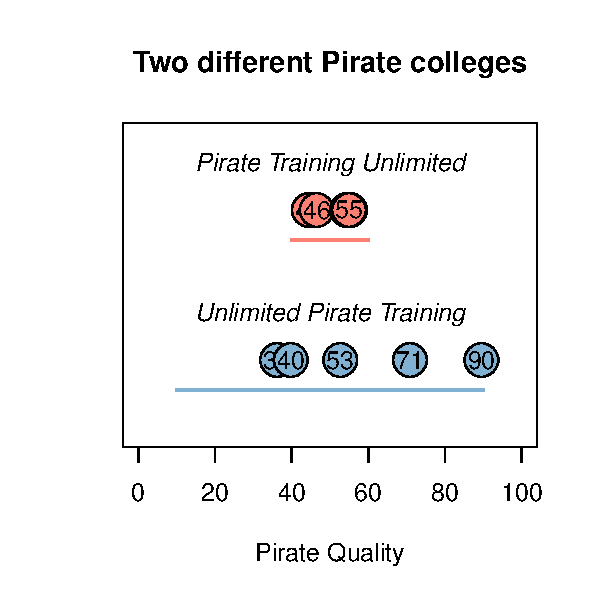
\includegraphics[width=\maxwidth]{figure/unnamed-chunk-32-1} 

\end{knitrout}
\end{tiny}
\caption{Sampling 5 potential pirates from two different pirate colleges. Pirate Training Unlimited (PTU) consistently produces average pirates (with scores between 40 and 60), while Unlimited Pirate Training (UPT), produces a wide range of pirates from 0 to 100.}
\label{fig:piratecollege}
\end{marginfigure}
By now you know how to generate sequences of numbers with the functions :, \texttt{seq()}, and \texttt{rep()}. However, these functions don't generate very interesting data. Instead, we can use R to generate randomly sampled data from specified \textit{probability distributions}. A probability distribution is simply an equation that indicates how likely certain numerical values are to be drawn. When you draw a \textit{sample} of size N from a distribution, you are selecting N numerical values drawn according to that distribution's likelihood function.

For example, imagine you need to hire a new group of pirates for your crew. You have the option of hiring people form one of two different pirate training colleges that produce pirates of varying quality. One college ``Pirate Training Unlimited" might tend to pirates that are generally ok - never great but never terrible. While another college ``Unlimited Pirate Training" might produce pirates with a wide variety of quality, from very low to very high. In Figure~\ref{fig:piratecollege} I plotted 5 example pirates from each college, where each pirate is shown as a ball with a number written on it. As you can see, pirates from PTU all tend to be clustered between 40 and 60 (not terrible but not great), whlie pirates from UPT are all over the map, from 0 to 100. We can use probability distributions (in this case, the uniform distribution) to 


%\marginnote{Mathematically, a probability distribution must satisfy two criteria: 1) All likelihoods must be positive, 2) The sum (or integral) of all likelihoods must equal 1.} 

In the next section we'll go over some of the most commonly used sampling distributions: the Normal and Uniform distributions.

\pagebreak
\subsection{The Normal (Gaussian) distribution}

\begin{marginfigure}
\begin{tiny}
\begin{knitrout}
\definecolor{shadecolor}{rgb}{0.969, 0.969, 0.969}\color{fgcolor}\begin{kframe}
\begin{alltt}
\hlkwd{require}\hlstd{(}\hlstr{"RColorBrewer"}\hlstd{)}

\hlcom{# Create blank plot}
\hlkwd{plot}\hlstd{(}\hlnum{1}\hlstd{,} \hlkwc{xlim} \hlstd{=} \hlkwd{c}\hlstd{(}\hlopt{-}\hlnum{5}\hlstd{,} \hlnum{5}\hlstd{),} \hlkwc{ylim} \hlstd{=} \hlkwd{c}\hlstd{(}\hlnum{0}\hlstd{,} \hlnum{1}\hlstd{),}
     \hlkwc{xlab} \hlstd{=} \hlstr{"x"}\hlstd{,} \hlkwc{ylab} \hlstd{=} \hlstr{"dnorm(x)"}\hlstd{,} \hlkwc{type} \hlstd{=} \hlstr{"n"}\hlstd{,}
     \hlkwc{main} \hlstd{=} \hlstr{"Three Normal Distributions"}
     \hlstd{)}

\hlcom{# Set up design matrix for loop}
\hlstd{design.matrix} \hlkwb{<-} \hlkwd{data.frame}\hlstd{(}\hlstr{"mean"} \hlstd{=} \hlkwd{c}\hlstd{(}\hlnum{0}\hlstd{,} \hlopt{-}\hlnum{2}\hlstd{,} \hlnum{1}\hlstd{),}
                            \hlstr{"sd"} \hlstd{=} \hlkwd{c}\hlstd{(}\hlnum{1}\hlstd{,} \hlnum{.5}\hlstd{,} \hlnum{2}\hlstd{)}
                            \hlstd{)}
\hlcom{# Set colors}
\hlstd{col.vec} \hlkwb{<-} \hlkwd{brewer.pal}\hlstd{(}\hlnum{10}\hlstd{,} \hlkwc{name} \hlstd{=} \hlstr{"Set3"}\hlstd{)[}\hlnum{4}\hlopt{:}\hlnum{6}\hlstd{]}

\hlcom{# Start loop over distributions}
\hlkwa{for} \hlstd{(i} \hlkwa{in} \hlnum{1}\hlopt{:}\hlkwd{nrow}\hlstd{(design.matrix)) \{}

\hlstd{mean.i} \hlkwb{<-} \hlstd{design.matrix}\hlopt{$}\hlstd{mean[i]}
\hlstd{sd.i} \hlkwb{<-} \hlstd{design.matrix}\hlopt{$}\hlstd{sd[i]}

\hlstd{fun} \hlkwb{<-} \hlkwa{function}\hlstd{(}\hlkwc{x}\hlstd{) \{}
  \hlkwd{dnorm}\hlstd{(x,} \hlkwc{mean} \hlstd{= mean.i,} \hlkwc{sd} \hlstd{= sd.i)\}}

\hlkwd{curve}\hlstd{(}\hlkwc{expr} \hlstd{= fun,}
      \hlkwc{from} \hlstd{=} \hlopt{-}\hlnum{5}\hlstd{,}\hlkwc{to} \hlstd{=} \hlnum{5}\hlstd{,}
      \hlkwc{xlab} \hlstd{=} \hlstr{"x"}\hlstd{,} \hlkwc{lwd} \hlstd{=} \hlnum{3}\hlstd{,}
      \hlkwc{add} \hlstd{= T,} \hlkwc{col} \hlstd{= col.vec[i])}

\hlstd{samples} \hlkwb{<-} \hlkwd{rnorm}\hlstd{(}\hlkwc{n} \hlstd{=} \hlnum{10}\hlstd{,} \hlkwc{mean} \hlstd{= mean.i,} \hlkwc{sd} \hlstd{= sd.i)}

\hlkwd{segments}\hlstd{(}\hlkwc{x0} \hlstd{= samples,} \hlkwc{y0} \hlstd{=} \hlkwd{rep}\hlstd{(}\hlnum{0}\hlstd{,} \hlnum{10}\hlstd{),}
         \hlkwc{x1} \hlstd{= samples,} \hlkwc{y1} \hlstd{=} \hlkwd{fun}\hlstd{(samples),}
         \hlkwc{col} \hlstd{= col.vec[i],} \hlkwc{lwd} \hlstd{=} \hlnum{1}\hlstd{,} \hlkwc{lty} \hlstd{=} \hlnum{2}
         \hlstd{)}
\hlstd{\}}

\hlstd{legend.fun} \hlkwb{<-} \hlkwa{function}\hlstd{(}\hlkwc{i}\hlstd{) \{}
  \hlkwd{paste}\hlstd{(}\hlstr{"mean = "}\hlstd{, design.matrix}\hlopt{$}\hlstd{mean[i],}
        \hlstr{", sd = "}\hlstd{, design.matrix}\hlopt{$}\hlstd{sd[i],} \hlkwc{sep} \hlstd{=} \hlstr{""}\hlstd{)\}}

\hlkwd{legend}\hlstd{(}\hlstr{"topright"}\hlstd{,}
       \hlkwc{legend} \hlstd{=} \hlkwd{c}\hlstd{(}\hlkwd{legend.fun}\hlstd{(}\hlnum{1}\hlstd{),}
                  \hlkwd{legend.fun}\hlstd{(}\hlnum{2}\hlstd{),}
                  \hlkwd{legend.fun}\hlstd{(}\hlnum{3}\hlstd{)}
                  \hlstd{),}
       \hlkwc{lwd} \hlstd{=} \hlkwd{rep}\hlstd{(}\hlnum{3}\hlstd{,} \hlnum{3}\hlstd{),}
       \hlkwc{col} \hlstd{= col.vec[}\hlnum{1}\hlopt{:}\hlnum{3}\hlstd{]}
       \hlstd{)}
\end{alltt}
\end{kframe}
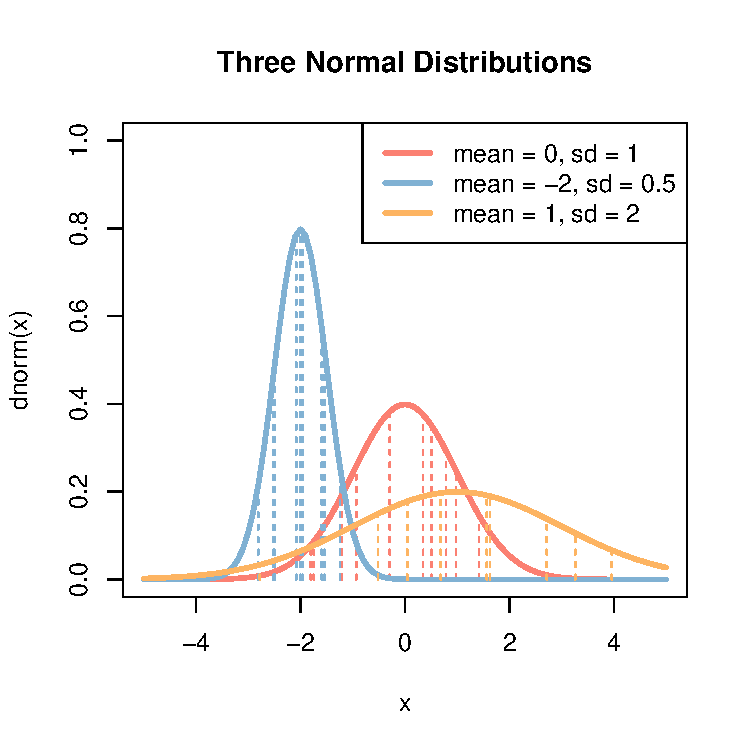
\includegraphics[width=\maxwidth]{figure/unnamed-chunk-33-1} 

\end{knitrout}
\caption{Three different normal distributions with different means and standard deviations.}
\label{fig:normaldist}
\end{tiny}
\end{marginfigure}
Let's start with the most famous distribution in statistics: the Normal (or if you want to sound pretentious, the Gaussian) distribution. The Normal distribution is bell-shaped, and has two parameters: a mean and a standard deviation. See the margin figure~\ref{fig:normaldist} for plots of three different Normal distributions with different means and standard deviations.


To generate samples from a normal distribution in R, we use the function \texttt{rnorm()} this function has three arguments:




\vspace{5mm} %5mm vertical space
\noindent
\setlength{\fboxrule}{1.5pt}
\fbox{
\parbox{\textwidth}{

\newfun{rnorm()}\index{rnorm()}

\hline

\begin{description}

\item[\tt{n}] \hfill \\
    The number of observations
\item[\tt{mean}] \hfill \\
    The mean of the Normal distribution from which samples are drawn (not the sample mean!!)
\item[\tt{sd}] \hfill \\
  The standard deviation of the Normal distribution from which samples are drawn
  
\end{description}

}
}
\vspace{5mm} %5mm vertical space


For example, let's draw 5 samples (\texttt{n = 5}) from a normal distribution with mean 0 (\texttt{mean = 0}) and standard deviation 1 (\texttt{sd = 1})

\begin{knitrout}
\definecolor{shadecolor}{rgb}{0.969, 0.969, 0.969}\color{fgcolor}\begin{kframe}
\begin{alltt}
\hlkwd{rnorm}\hlstd{(}\hlkwc{n} \hlstd{=} \hlnum{5}\hlstd{,} \hlkwc{mean} \hlstd{=} \hlnum{0}\hlstd{,} \hlkwc{sd} \hlstd{=} \hlnum{1}\hlstd{)}
\end{alltt}
\begin{verbatim}
## [1]  0.375799 -1.367125 -1.289852 -1.430844 -2.457182
\end{verbatim}
\end{kframe}
\end{knitrout}

This code returns a vector of 5 values, where each value is a new random sample drawn from a Normal distribution with mean = 0 and standard deviation = 1.

Because the sampling is done randomly, you'll get different values each time you run the \texttt{rnorm()} (or any other random sampling) function. To see this, let's create two different sets of samples from a normal distribution with mean 10 and standard deviation 5 and see how they compare:

\begin{knitrout}
\definecolor{shadecolor}{rgb}{0.969, 0.969, 0.969}\color{fgcolor}\begin{kframe}
\begin{alltt}
\hlstd{a} \hlkwb{<-} \hlkwd{rnorm}\hlstd{(}\hlnum{5}\hlstd{,} \hlkwc{mean} \hlstd{=} \hlnum{10}\hlstd{,} \hlkwc{sd} \hlstd{=} \hlnum{5}\hlstd{)}
\hlstd{b} \hlkwb{<-} \hlkwd{rnorm}\hlstd{(}\hlnum{5}\hlstd{,} \hlkwc{mean} \hlstd{=} \hlnum{10}\hlstd{,} \hlkwc{sd} \hlstd{=} \hlnum{5}\hlstd{)}
\hlstd{a} \hlcom{# print a}
\end{alltt}
\begin{verbatim}
## [1]  8.752808  9.329998 11.479484 16.710223  3.270555
\end{verbatim}
\begin{alltt}
\hlstd{b} \hlcom{# print b}
\end{alltt}
\begin{verbatim}
## [1]  7.159241 20.320119 13.405458  5.809321  5.997274
\end{verbatim}
\end{kframe}
\end{knitrout}


As you can see, even though I used the exact same code to generate the vectors \texttt{a} and \texttt{b}, the numbers in each sample are different. That's because the samples are each drawn randomly and independently from the normal distribution. To visualize the sampling process, run the code in the margin Figure~\ref{fig:normaldist} on your machine several times. You should see the sampling lines dance around the distribution. 

\subsection{The Uniform distribution}

Next, let's move on to the \textit{uniform} distribution. The uniform distribution gives equal probability to all values between the minimum and maximum values.

\begin{marginfigure}
\begin{tiny}
\begin{knitrout}
\definecolor{shadecolor}{rgb}{0.969, 0.969, 0.969}\color{fgcolor}\begin{kframe}
\begin{alltt}
\hlcom{# uniform distribution}
\hlkwd{curve}\hlstd{(dunif,}
      \hlkwc{from} \hlstd{=} \hlnum{0}\hlstd{,} \hlkwc{to} \hlstd{=} \hlnum{1}\hlstd{,}
      \hlkwc{xlim} \hlstd{=} \hlkwd{c}\hlstd{(}\hlopt{-}\hlnum{.5}\hlstd{,} \hlnum{1.5}\hlstd{),}
      \hlkwc{xlab} \hlstd{=} \hlstr{"x"}\hlstd{,}
      \hlkwc{lwd} \hlstd{=} \hlnum{2}\hlstd{,}
      \hlkwc{main} \hlstd{=} \hlstr{"Uniform\textbackslash{}nmin = 0, max = 1"}\hlstd{)}
\end{alltt}
\end{kframe}
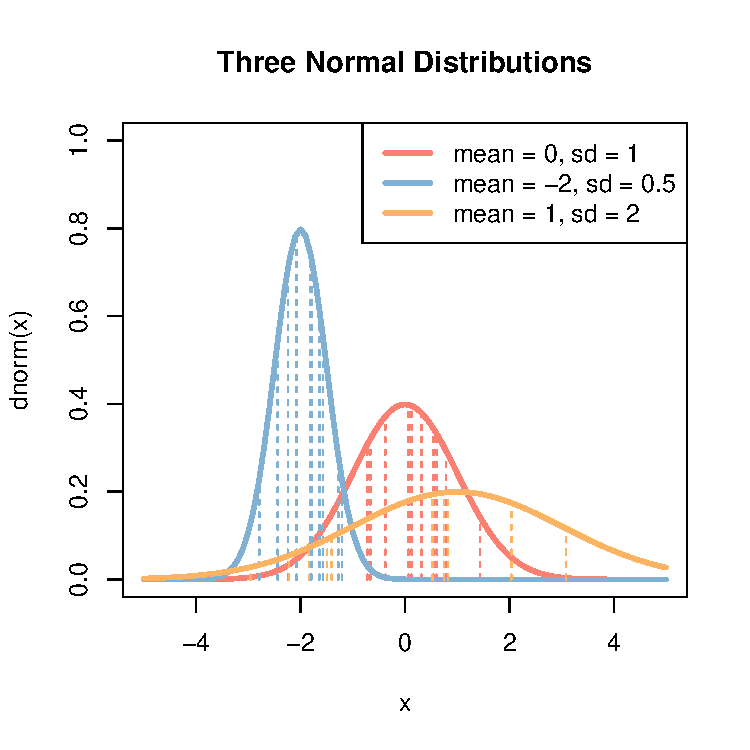
\includegraphics[width=\maxwidth]{figure/unnamed-chunk-36-1} 

\end{knitrout}
\caption{The Uniform distribution - known colloquially as the Anthony Davis distribution.}
\label{fig:unif_dist}
\end{tiny}
\end{marginfigure}


To generate samples from a uniform distribution, we use the function \texttt{runif()}, the function has 3 arguments:

\vspace{5mm} %5mm vertical space
\noindent
\setlength{\fboxrule}{1.5pt}
\fbox{
\parbox{\textwidth}{

\newfun{runif()}\index{runif()}

\hline

\begin{description}

\item[\tt{n}] \hfill \\
    The number of observations (i.e.; samples)
\item[\tt{min}] \hfill \\
    The lower bound of the Uniform distribution from which samples are drawn
\item[\tt{max}] \hfill \\
    The upper bound of the Uniform distribution from which samples are drawn
\end{description}

}
}
\vspace{5mm} %5mm vertical space




Let's draw 5 samples from two uniform distributions, one with bounds at 0 and 1, and one with bounds at -100 and 100:

\begin{footnotesize}
\begin{knitrout}
\definecolor{shadecolor}{rgb}{0.969, 0.969, 0.969}\color{fgcolor}\begin{kframe}
\begin{alltt}
\hlkwd{runif}\hlstd{(}\hlnum{5}\hlstd{,} \hlkwc{min} \hlstd{=} \hlnum{0}\hlstd{,} \hlkwc{max} \hlstd{=} \hlnum{1}\hlstd{)} \hlcom{# 5 samples from U[0, 1]}
\end{alltt}
\begin{verbatim}
## [1] 0.001454292 0.919849717 0.580778579 0.693033657 0.306065331
\end{verbatim}
\begin{alltt}
\hlkwd{runif}\hlstd{(}\hlnum{5}\hlstd{,} \hlkwc{min} \hlstd{=} \hlopt{-}\hlnum{100}\hlstd{,} \hlkwc{max} \hlstd{=} \hlnum{100}\hlstd{)} \hlcom{# 5 samples from U[-100, 100]}
\end{alltt}
\begin{verbatim}
## [1] 35.446931 53.111058 60.491567 -3.057751 13.683292
\end{verbatim}
\end{kframe}
\end{knitrout}
\end{footnotesize}

\subsection{Sampling from a set of values: sample()}

The next function we'll use is \textbf{sample()}. The sample function works a bit differently from \texttt{runif()} and \texttt{rnorm()} because it allows to you to define which values you want to sample and the probability associated with each value. For example, if you want to simulate the flip of a fair coin, you can tell the sample function to draw the value "Heads" with probability .50, and the value "Tails" with probability .50.


\vspace{5mm} %5mm vertical space
\noindent
\setlength{\fboxrule}{1.5pt}
\fbox{
\parbox{\textwidth}{

\newfun{sample()}\index{sample()}

\hline

\begin{description}

\item[\tt{x}] \hfill \\
    A vector of outcomes you want to sample from. For example, to simulate coin flips, you'd enter \texttt{x = c("Heads", "Tails")}
\item[\tt{size}] \hfill \\
    The number of samples you want to draw.
\item[\tt{replace}] \hfill \\
    Should sampling be done with replacement? If T, then each individual sample will be replaced in the data vector. If F, then the same outcome will never be drawn more than once. Think about replacement like drawing different balls from a bag. Sampling with replacement (\texttt{replace = T}) means that each time you draw a ball, you return the ball back into the bag before drawing another ball. Sampling without replacement (\texttt{replace = F}) means that after you draw a ball, you remove that ball from the bag before drawing again.
\item[\tt{prob}] \hfill \\
    A vector of probabilities of the same length as \texttt{x} indicating how likely each outcome in "x" is. For example, to sample equally from two outcomes, you'd enter \texttt{prob = c(.5, .5)}. The first value corresponds to the first value of x and the second corresponds to the second value (etc.). The vector of probabilities you give as an argument should add up to one. However, if they don't, R will just rescale them so that they will sum to 1.
    
\end{description}

}
}
\vspace{5mm} %5mm vertical space


As a simple example, let's simulate 10 flips of a fair coin, were the probably of getting either a Head or Tail is .50:

\begin{footnotesize}
\begin{knitrout}
\definecolor{shadecolor}{rgb}{0.969, 0.969, 0.969}\color{fgcolor}\begin{kframe}
\begin{alltt}
\hlkwd{sample}\hlstd{(}\hlkwc{x} \hlstd{=} \hlkwd{c}\hlstd{(}\hlstr{"Heads"}\hlstd{,} \hlstr{"Tails"}\hlstd{),} \hlcom{# The values you want to sample from}
       \hlkwc{size} \hlstd{=} \hlnum{10}\hlstd{,}  \hlcom{# The number of samples}
       \hlkwc{prob} \hlstd{=} \hlkwd{c}\hlstd{(}\hlnum{.5}\hlstd{,} \hlnum{.5}\hlstd{),} \hlcom{# The probability of each value}
       \hlkwc{replace} \hlstd{= T} \hlcom{# Sampling with replacement}
       \hlstd{)}
\end{alltt}
\begin{verbatim}
##  [1] "Heads" "Heads" "Tails" "Heads" "Tails" "Tails" "Tails" "Tails"
##  [9] "Tails" "Heads"
\end{verbatim}
\end{kframe}
\end{knitrout}
\end{footnotesize}

As you can see, our function returned a vector of 10 values corresponding to our sample size of 10. Keep in mind that, just like using \texttt{rnorm()} and \texttt{runif()}, the \texttt{sample()} function can give you different outcomes every time you run it.


\begin{marginfigure}
\begin{tiny}
\begin{knitrout}
\definecolor{shadecolor}{rgb}{0.969, 0.969, 0.969}\color{fgcolor}\begin{kframe}
\begin{alltt}
\hlkwd{par}\hlstd{(}\hlkwc{mar} \hlstd{=} \hlkwd{c}\hlstd{(}\hlnum{3}\hlstd{,} \hlnum{3}\hlstd{,} \hlnum{3}\hlstd{,} \hlnum{3}\hlstd{))}
\hlkwd{plot}\hlstd{(}\hlnum{1}\hlstd{,} \hlkwc{xlim} \hlstd{=} \hlkwd{c}\hlstd{(}\hlnum{0}\hlstd{,} \hlnum{1}\hlstd{),} \hlkwc{ylim} \hlstd{=} \hlkwd{c}\hlstd{(}\hlnum{0}\hlstd{,} \hlnum{1}\hlstd{),}
     \hlkwc{xlab} \hlstd{=} \hlstr{""}\hlstd{,} \hlkwc{ylab} \hlstd{=} \hlstr{""}\hlstd{,} \hlkwc{xaxt} \hlstd{=} \hlstr{"n"}\hlstd{,}
     \hlkwc{yaxt} \hlstd{=} \hlstr{"n"}\hlstd{,} \hlkwc{type} \hlstd{=} \hlstr{"n"}\hlstd{,}
     \hlkwc{main} \hlstd{=} \hlstr{"Chest of 20 Gold, 30 Silver,\textbackslash{}nand 50 Bronze Coins"}\hlstd{)}

\hlkwd{points}\hlstd{(}\hlkwd{runif}\hlstd{(}\hlnum{100}\hlstd{,} \hlnum{.1}\hlstd{,} \hlnum{.9}\hlstd{),}
       \hlkwd{runif}\hlstd{(}\hlnum{100}\hlstd{,} \hlnum{.1}\hlstd{,} \hlnum{.9}\hlstd{),}
       \hlkwc{pch} \hlstd{=} \hlnum{21}\hlstd{,} \hlkwc{cex} \hlstd{=} \hlnum{3}\hlstd{,}
       \hlkwc{bg} \hlstd{=} \hlkwd{c}\hlstd{(}\hlkwd{rep}\hlstd{(}\hlstr{"gold"}\hlstd{,} \hlnum{20}\hlstd{),}
              \hlkwd{rep}\hlstd{(}\hlstr{"gray94"}\hlstd{,} \hlnum{30}\hlstd{),}
              \hlkwd{rep}\hlstd{(}\hlstr{"chocolate"}\hlstd{,} \hlnum{50}\hlstd{))}
       \hlstd{)}
\end{alltt}
\end{kframe}
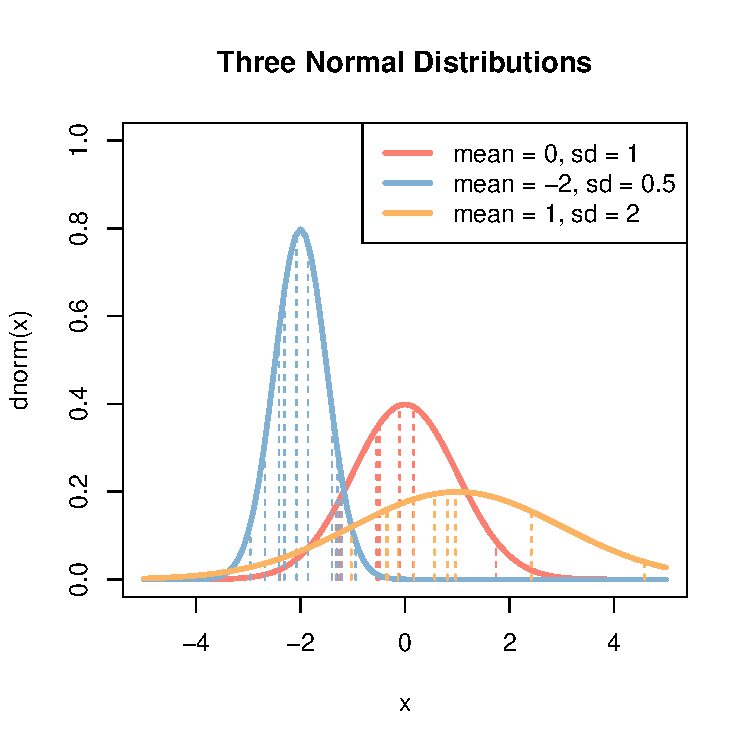
\includegraphics[width=\maxwidth]{figure/unnamed-chunk-39-1} 

\end{knitrout}
\end{tiny}
\end{marginfigure}

\subsection{Drawing coins from a treasure chest}

Now, let's sample drawing coins from a treasure chest Let's say the chest has 100 coins: 20 gold, 30 silver, and 50 bronze. Let's draw 10 random coins from this chest. Because we remove coins when we draw them, we'll set \texttt{replace = F}.

\begin{knitrout}
\definecolor{shadecolor}{rgb}{0.969, 0.969, 0.969}\color{fgcolor}\begin{kframe}
\begin{alltt}
\hlcom{# Create chest with the 100 coins}

\hlstd{chest} \hlkwb{<-} \hlkwd{c}\hlstd{(}\hlkwd{rep}\hlstd{(}\hlstr{"gold"}\hlstd{,} \hlnum{20}\hlstd{),}
         \hlkwd{rep}\hlstd{(}\hlstr{"silver"}\hlstd{,} \hlnum{30}\hlstd{),}
         \hlkwd{rep}\hlstd{(}\hlstr{"bronze"}\hlstd{,} \hlnum{50}\hlstd{)}
         \hlstd{)}

\hlcom{# Draw 10 coins from the chest without replacement}

\hlkwd{sample}\hlstd{(}\hlkwc{x} \hlstd{= chest,}
       \hlkwc{size} \hlstd{=} \hlnum{10}\hlstd{,}
       \hlkwc{prob} \hlstd{=} \hlkwd{rep}\hlstd{(}\hlnum{1} \hlopt{/} \hlnum{100}\hlstd{,} \hlkwc{times} \hlstd{=} \hlnum{100}\hlstd{),}
       \hlkwc{replace} \hlstd{= F}
       \hlstd{)}
\end{alltt}
\begin{verbatim}
##  [1] "bronze" "silver" "bronze" "bronze" "silver" "bronze" "bronze"
##  [8] "bronze" "bronze" "silver"
\end{verbatim}
\end{kframe}
\end{knitrout}

The output of the \texttt{sample()} function above is a vector of 10 strings indicating the type of coin we drew on each sample. The order of these strings matter: the first one is the first coin we drew, and the last one is the 10th coin we drew. And like any random sampling function, this code will likely give you different results everytime you run it! See how long it takes you to get 10 gold coins...

\subsection{Simulating Pinder Outcomes}

\begin{marginfigure}
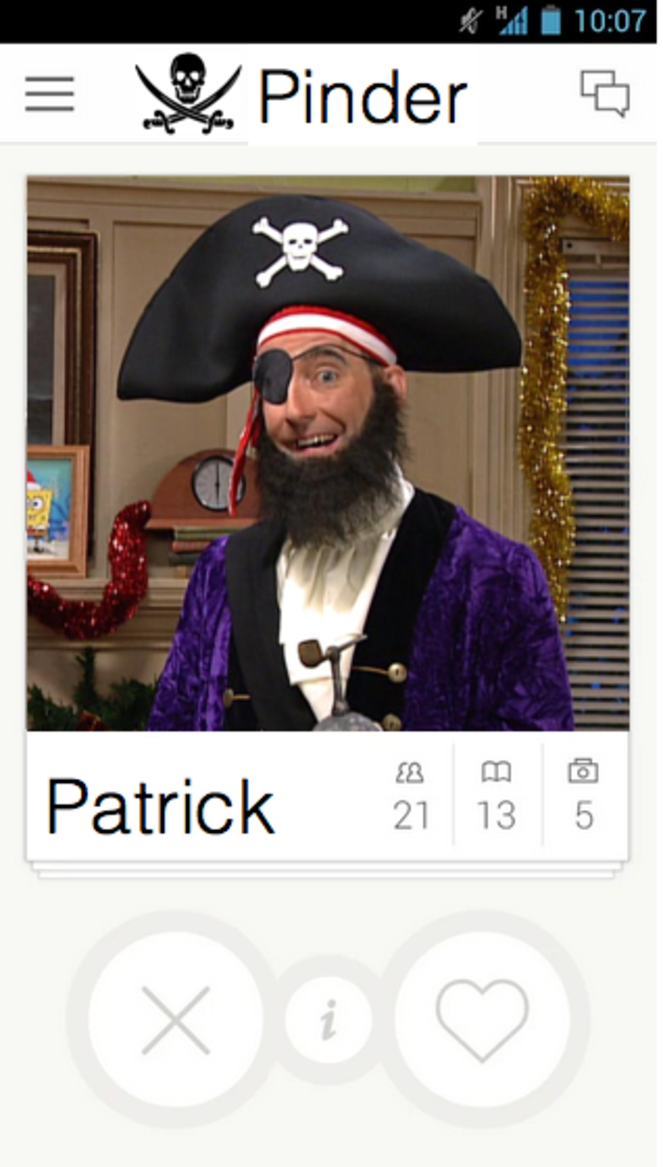
\includegraphics[width=\linewidth]{/Users/Nathaniel/Dropbox/Git/YaRrr_Book/media/pinder.pdf}
\caption{A typical Pinder profile.}
\label{fig:pinder}
\end{marginfigure}


Let's simulate some Pinder outcomes. For those who don't know, Pinder is an app that allows Pirates to view profiles of potential dates. For each potential date, you can see their picture and either "like" them by swiping right, or "dislike" them by swiping left. If a pirate that you "liked" also "likes" you, then you've had a successful match and will be able to start chatting. let's say you "swipe right" on 20 Pinder profiles and the probability you get a match is 20\%. We can simulate this using the sample function

\begin{footnotesize}
\begin{knitrout}
\definecolor{shadecolor}{rgb}{0.969, 0.969, 0.969}\color{fgcolor}\begin{kframe}
\begin{alltt}
\hlkwd{sample}\hlstd{(}\hlkwc{x} \hlstd{=} \hlkwd{c}\hlstd{(}\hlstr{"Match!!!"}\hlstd{,} \hlstr{"No Match"}\hlstd{),}
       \hlkwc{size} \hlstd{=} \hlnum{20}\hlstd{,}
       \hlkwc{replace} \hlstd{= T,} \hlcom{# Replace each sample back to the set}
       \hlkwc{prob} \hlstd{=} \hlkwd{c}\hlstd{(}\hlnum{.2}\hlstd{,} \hlnum{.8}\hlstd{)}  \hlcom{# Probability of Match! is .2, and No Match :( is .8)}
       \hlstd{)}
\end{alltt}
\begin{verbatim}
##  [1] "No Match" "Match!!!" "No Match" "Match!!!" "No Match" "No Match"
##  [7] "No Match" "No Match" "No Match" "No Match" "No Match" "No Match"
## [13] "No Match" "Match!!!" "Match!!!" "No Match" "Match!!!" "No Match"
## [19] "No Match" "Match!!!"
\end{verbatim}
\end{kframe}
\end{knitrout}
\end{footnotesize}

The output of this function is a simulated response from 10 pirates that you liked. 

%In the example above I set \texttt{replace = T}. If I didn't do this, then on the third sample R would run out of objects to draw from. However, there are cases where we would not want sampling with replacement: for example, when deciding where to go clubbing in Berlin...

%' \subsection{Where should I go clubbing in Berlin...?}
%' 
%' 
%' \begin{marginfigure}
%' \begin{tiny}
%' <<fig.width = 4, fig.height = 4>>=
%' par(mar = c(4, 4, 4, 4))
%'     
%' plot(1, xlim = c(0, 1), ylim = c(0, 1), 
%'      xlab = "", ylab = "", xaxt = "n", 
%'      yaxt = "n", type = "n", main = "Bag of clubs")
%' 
%' x.vals <- runif(5, .1, .9)
%' y.vals <- runif(5, .1, .7)
%' clubs <- c("Berghain", "Club der\nVisionare", 
%'              "Goldengate", "Watergate", "Keller")
%' for (i in 1:5) {
%' 
%' points(x.vals[i], 
%'        y.vals[i],
%'        pch = 21, cex = 13, bg = "white", lwd = 2
%'        )
%' 
%' 
%' text(x.vals[i], y.vals[i], 
%'      labels = clubs[i], cex = .8)
%'   }
%' @
%' \end{tiny}
%' \end{marginfigure}
%' 
%' Let's say you planning a weekend of clubbing in Berlin and need to decide on just 2 out of 5 clubs to visit. Since we don't want to visit the same club twice, we'll set \texttt{replace = F}. Additionally, because we want each of the clubs to be equally likely to be selected, we'll set the \texttt{prob} argument as a vector of five 1/5 values.
%' 
%' \begin{footnotesize}
%' <<>>=
%' clubs <- sample(x = c("Berghain", "Club der Visionare", 
%'              "Goldengate", "Watergate", "Keller"),
%'        size = 2,
%'        replace = F,
%'        prob = c(1/5, 1/5, 1/5, 1/5, 1/5) # Set the probability of each to 1/5
%'        )
%' clubs
%' @
%' \end{footnotesize}
%' 
%' Looks like R has selected clubs[1] and clubs[2]. Let's see if we even make it to clubs[2]...

\section{Descriptive statistics}

Ok, now that we can generate some data, let's learn the basic descriptive statistics functions. We'll focus on the most common ones for numerical analyses.


\vspace{5mm} %5mm vertical space
\noindent
\setlength{\fboxrule}{1.5pt}
\fbox{
\parbox{\textwidth}{

\newfun{Common Descriptive Statistics}

\hline

\begin{description}

\item[\tt{mean(x)}] \hfill \\
    The arithmetic mean of a vector x
\item[\tt{median(x)}] \hfill \\
    The median of a vector x. 50\% of the data should be less than \texttt{median(x)} and 50\% should be greater than \texttt{median(x)}.
\item[\tt{sd(x), var(x)}] \hfill \\
    The standard deviation and variance of a vector x.
\item[\tt{min(x), max(x)}] \hfill \\
    The minimum and maximum values of a vector x
\item[\tt{quantile(x, p)}] \hfill \\
    The pth sample quantile of a vector x. For example, \texttt{quantile(x, .2)} will tell you the value at which 20\% of cases are less than x. The function \texttt{quantile(x, .5)} is identical to \texttt{median(x)}
\item[\tt{summary(x)}] \hfill \\ 
  Shows you several descriptive statistics of a vector x, including \texttt{min(x)}, \texttt{max(x)}, \texttt{median(x)}, \texttt{mean(x)}
  
\end{description}

}
}
\vspace{5mm} %5mm vertical space


Each of these functions takes a vector as an argument, and returns a scalar as a result. Let's calculate some descriptive statistics from some pirate related data. I'll create a vector called \texttt{data} that contains the number of tattoos from 10 random pirates

\begin{knitrout}
\definecolor{shadecolor}{rgb}{0.969, 0.969, 0.969}\color{fgcolor}\begin{kframe}
\begin{alltt}
\hlstd{tattoos} \hlkwb{<-} \hlkwd{c}\hlstd{(}\hlnum{4}\hlstd{,} \hlnum{50}\hlstd{,} \hlnum{2}\hlstd{,} \hlnum{39}\hlstd{,} \hlnum{4}\hlstd{,} \hlnum{20}\hlstd{,} \hlnum{4}\hlstd{,} \hlnum{8}\hlstd{,} \hlnum{10}\hlstd{,} \hlnum{100}\hlstd{)}
\end{alltt}
\end{kframe}
\end{knitrout}

To calculate the mean of the data, we simply write:

\begin{knitrout}
\definecolor{shadecolor}{rgb}{0.969, 0.969, 0.969}\color{fgcolor}\begin{kframe}
\begin{alltt}
\hlkwd{mean}\hlstd{(tattoos)}
\end{alltt}
\begin{verbatim}
## [1] 24.1
\end{verbatim}
\end{kframe}
\end{knitrout}

The other descriptive statistics functions are just as easy: Let's test the \texttt{median()}, \texttt{sd()}, \textt{min()}, and \texttt{max()} functions:

\begin{footnotesize}
\begin{knitrout}
\definecolor{shadecolor}{rgb}{0.969, 0.969, 0.969}\color{fgcolor}\begin{kframe}
\begin{alltt}
\hlkwd{median}\hlstd{(tattoos)}
\end{alltt}
\begin{verbatim}
## [1] 9
\end{verbatim}
\begin{alltt}
\hlkwd{sd}\hlstd{(tattoos)}
\end{alltt}
\begin{verbatim}
## [1] 31.32074
\end{verbatim}
\begin{alltt}
\hlkwd{min}\hlstd{(tattoos)}
\end{alltt}
\begin{verbatim}
## [1] 2
\end{verbatim}
\begin{alltt}
\hlkwd{max}\hlstd{(tattoos)}
\end{alltt}
\begin{verbatim}
## [1] 100
\end{verbatim}
\end{kframe}
\end{knitrout}
\end{footnotesize}

One important point about the descriptive statistics functions is that most (if not all) of them as a default will freak out if there is a missing (NA) value in the data. For example, the following code will return NA as a result because there is an NA value in the data vector:

\marginnote{Include the argument \textt{na.rm = T} to ignore missing (NA) values when calculating a descriptive statistic.}

\begin{knitrout}
\definecolor{shadecolor}{rgb}{0.969, 0.969, 0.969}\color{fgcolor}\begin{kframe}
\begin{alltt}
\hlkwd{mean}\hlstd{(}\hlkwd{c}\hlstd{(}\hlnum{1}\hlstd{,} \hlnum{5}\hlstd{,} \hlnum{NA}\hlstd{,} \hlnum{2}\hlstd{))}
\end{alltt}
\begin{verbatim}
## [1] NA
\end{verbatim}
\end{kframe}
\end{knitrout}

To tell a descriptive statistic function to ignore missing (NA) values, include the argument \texttt{na.rm = T} in the function:

\begin{knitrout}
\definecolor{shadecolor}{rgb}{0.969, 0.969, 0.969}\color{fgcolor}\begin{kframe}
\begin{alltt}
\hlkwd{mean}\hlstd{(}\hlkwd{c}\hlstd{(}\hlnum{1}\hlstd{,} \hlnum{5}\hlstd{,} \hlnum{NA}\hlstd{,} \hlnum{2}\hlstd{),} \hlkwc{na.rm} \hlstd{= T)}
\end{alltt}
\begin{verbatim}
## [1] 2.666667
\end{verbatim}
\end{kframe}
\end{knitrout}

Now, the function will ignore NA and calculate the mean of the non-missing values. While this may seem trivial now (why did we include an NA value in the vector if we wanted to ignore it?!), it will be become very important when we apply the function to large existing datasets that may contain missing values.

If you want to get many summary statistics from a vector, you can use the \textbf{summary()} function which gives you several key statistics:

\begin{footnotesize}
\begin{knitrout}
\definecolor{shadecolor}{rgb}{0.969, 0.969, 0.969}\color{fgcolor}\begin{kframe}
\begin{alltt}
\hlkwd{summary}\hlstd{(tattoos)}
\end{alltt}
\begin{verbatim}
##    Min. 1st Qu.  Median    Mean 3rd Qu.    Max. 
##    2.00    4.00    9.00   24.10   34.25  100.00
\end{verbatim}
\end{kframe}
\end{knitrout}
\end{footnotesize}





\subsection{Other helpful vector functions}

Here are some other functions that you will find useful when managing numeric vectors:


\vspace{5mm} %5mm vertical space
\noindent
\setlength{\fboxrule}{1.5pt}
\fbox{
\parbox{\textwidth}{

\newfun{Other helpful numeric functions}

\hline

\begin{description}

\item[\tt{round(x, digits)}] \hfill \\
    Round values in a vector (or scaler) x to a certain number of digits.
\item[\tt{ceiling(x), floor(x)}] \hfill \\
   Round a number to the next largest integer with \texttt{ceiling(x)} or down to the next lowest integer with \texttt{floor(x)}.
\item[\tt{x \%\% y}] \hfill \\
    Modular arithmetic (i.e.; x mod y). You can interpret \texttt{x \%\% y} as ``What is the remainder after dividing x by y?" For example, \texttt{10 \%\% 3} equals 1 because 3 times 3 is 9 (which leaves a remainder of 1).
\end{description}

}
}
\vspace{5mm} %5mm vertical space


\section{A worked example: A quick test of the law of large numbers}

According to the law of large numbers, the larger our sample size, the closer our sample mean should be to the population mean. In other words, the more data (samples) you have, the more accurate your estimate should be. Let's test this by drawing either a small (N = 10) or a large (N = 1,000,000) number of observations from a Normal distribution with mean = 100 and sd = 20:

\marginnote{Tip: You can easily write large powers of 10 by using the notation \texttt{1eN}, where N is the power of 10. For example: \texttt{1e6} is the same as 1,000,000}

\begin{footnotesize}
\begin{knitrout}
\definecolor{shadecolor}{rgb}{0.969, 0.969, 0.969}\color{fgcolor}\begin{kframe}
\begin{alltt}
\hlstd{small} \hlkwb{<-} \hlkwd{rnorm}\hlstd{(}\hlnum{10}\hlstd{,} \hlkwc{mean} \hlstd{=} \hlnum{100}\hlstd{,} \hlkwc{sd} \hlstd{=} \hlnum{20}\hlstd{)} \hlcom{# 10 observations}
\hlstd{large} \hlkwb{<-} \hlkwd{rnorm}\hlstd{(}\hlnum{1e6}\hlstd{,} \hlkwc{mean} \hlstd{=} \hlnum{100}\hlstd{,} \hlkwc{sd} \hlstd{=} \hlnum{20}\hlstd{)} \hlcom{# One million observations}
\end{alltt}
\end{kframe}
\end{knitrout}
\end{footnotesize}

If our test worked, then the difference for the small sample should be larger than the large sample. Let's test this by calculating the mean of each sample and see how close they are to the true population mean of 100:

\begin{footnotesize}
\begin{knitrout}
\definecolor{shadecolor}{rgb}{0.969, 0.969, 0.969}\color{fgcolor}\begin{kframe}
\begin{alltt}
\hlkwd{mean}\hlstd{(small)} \hlcom{# What is the mean of the small sample?}
\end{alltt}
\begin{verbatim}
## [1] 97.75108
\end{verbatim}
\begin{alltt}
\hlkwd{mean}\hlstd{(large)} \hlcom{# What is the mean of the large sample?}
\end{alltt}
\begin{verbatim}
## [1] 100.0157
\end{verbatim}
\begin{alltt}
\hlkwd{mean}\hlstd{(small)} \hlopt{-} \hlnum{100} \hlcom{# How far is the mean of Small from 100?}
\end{alltt}
\begin{verbatim}
## [1] -2.248922
\end{verbatim}
\begin{alltt}
\hlkwd{mean}\hlstd{(large)} \hlopt{-} \hlnum{100} \hlcom{# How far is the mean of Large from 100?}
\end{alltt}
\begin{verbatim}
## [1] 0.01570442
\end{verbatim}
\end{kframe}
\end{knitrout}
\end{footnotesize}

Looks like the law of large numbers holds up!

\subsection{Additional Tips}


%----------------------------------------------------------------------------------------
%	CHAPTER 4
%----------------------------------------------------------------------------------------

\chapter{4: Indexing and comparing vectors}
\label{ch:4}


Chapter Goals:

\begin{enumerate}
  \item Use brackets [] and logical vectors to index vectors
  \item Combine indexing with descriptive statistics
  \item Learn indexing functions which(), sort()
  \item Vector discrete summary functions table() and unique()
  \item Set functions: intersect(), union(), setdiff(), %in%
\end{enumerate}


\section{Indexing vectors with brackets}

\marginnote{\textbf{Indexing with brackets [ ]} \\ To get the ith value of a vector called \texttt{vec}, use the bracket notation \textt{vec[i]}}

When we have a vector, we will frequently want to access specific values of a vector. These might be values in a specific location in the vector (i.e.; the fifth element) or based on some criteria (i.e.; all values greater than 0). We can accomplish this using indexing.

\newfun{vector[index]}\index{[]}

There are two main ways that you can use indexing to access subsets of data in a vector: numerical and logical indexing.

\subsection{Numerical Indexing}

With numerical indexing, you enter the integers corresponding to the values in the vector you want to access in the form \textt{data[num.index]}, where \texttt{data} is the data vector, and \texttt{num.index} is a vector of index values. For example, to get the first value in a vector, you'd write \texttt{data[1]}. To get the first, second, and third value, you can either type \texttt{data[c(1, 2, 3)} or \texttt{data[1:3]}.

Let's do a few more examples. We'll use the \texttt{tattoos} vector again and use indexing to extract specific values:
  
\begin{footnotesize}
\begin{knitrout}
\definecolor{shadecolor}{rgb}{0.969, 0.969, 0.969}\color{fgcolor}\begin{kframe}
\begin{alltt}
\hlstd{tattoos} \hlkwb{<-} \hlkwd{c}\hlstd{(}\hlnum{0}\hlstd{,} \hlnum{50}\hlstd{,} \hlnum{2}\hlstd{,} \hlnum{39}\hlstd{,} \hlnum{9}\hlstd{,} \hlnum{20}\hlstd{,} \hlnum{17}\hlstd{,} \hlnum{8}\hlstd{,} \hlnum{10}\hlstd{,} \hlnum{100}\hlstd{)}
\hlstd{tattoos[}\hlnum{1}\hlstd{]} \hlcom{# First element of tattoos}
\end{alltt}
\begin{verbatim}
## [1] 0
\end{verbatim}
\begin{alltt}
\hlstd{tattoos[}\hlnum{1}\hlopt{:}\hlnum{5}\hlstd{]} \hlcom{# 1-5 elements of tattoos}
\end{alltt}
\begin{verbatim}
## [1]  0 50  2 39  9
\end{verbatim}
\end{kframe}
\end{knitrout}

If you have defined an object that is a vector of integers, you can then index a variable using that vector. For example, let's define an object called \texttt{index} and use this object to index our data vector:
  
\begin{footnotesize}
\begin{knitrout}
\definecolor{shadecolor}{rgb}{0.969, 0.969, 0.969}\color{fgcolor}\begin{kframe}
\begin{alltt}
\hlstd{get.these.values} \hlkwb{<-} \hlnum{6}\hlopt{:}\hlnum{10}
\hlstd{tattoos[get.these.values]} \hlcom{# Indexing with a named object}
\end{alltt}
\begin{verbatim}
## [1]  20  17   8  10 100
\end{verbatim}
\end{kframe}
\end{knitrout}
\end{footnotesize}

You can also get random values from a vector by indexing a vector with the \texttt{sample()} function. Let's get 3 random values from the \texttt{tattoo} vector in 2 steps. First, we'll create 3 random indexing values using \texttt{sample()}. Secind, we'll index the \texttt{tattoo} object with the indexing values we generated in the first step.

\begin{footnotesize}
\begin{knitrout}
\definecolor{shadecolor}{rgb}{0.969, 0.969, 0.969}\color{fgcolor}\begin{kframe}
\begin{alltt}
\hlstd{rand.values} \hlkwb{<-} \hlkwd{sample}\hlstd{(}\hlkwc{x} \hlstd{=} \hlnum{1}\hlopt{:}\hlkwd{length}\hlstd{(tattoos),}  \hlcom{# Step 1: Determine indexing values}
                      \hlkwc{size} \hlstd{=} \hlnum{3}\hlstd{,}
                      \hlkwc{replace} \hlstd{= F)}

\hlstd{tattoos[rand.values]} \hlcom{# Step 2: Index tattoo with rand.values}
\end{alltt}
\begin{verbatim}
## [1] 20 10 50
\end{verbatim}
\end{kframe}
\end{knitrout}
\end{footnotesize}

The result of our indexing is 3 randomly selected values from the \texttt{tattoos} vector. Of course, we also could have done the same thing in one step by just entering \texttt{tattoos} as an argument to \texttt{sample()} like this:

\begin{footnotesize}
\begin{knitrout}
\definecolor{shadecolor}{rgb}{0.969, 0.969, 0.969}\color{fgcolor}\begin{kframe}
\begin{alltt}
\hlkwd{sample}\hlstd{(}\hlkwc{x} \hlstd{= tattoos,} \hlkwc{size} \hlstd{=} \hlnum{3}\hlstd{,} \hlkwc{replace} \hlstd{= F)}
\end{alltt}
\begin{verbatim}
## [1] 50 39  0
\end{verbatim}
\end{kframe}
\end{knitrout}
\end{footnotesize}

As you gain more experience with R, you'll realise that there are many ways to program the same result. The choice of which code you use comes down to a delicate balance of readability (How easily can your future self, and other people, understand what the code is doing?), simplicity (How many lines of code are necessary?), and processing speed (How quickly will R complete the task?).

\section{Creating logical vectors}


\begin{marginfigure}
\begin{tiny}
\begin{knitrout}
\definecolor{shadecolor}{rgb}{0.969, 0.969, 0.969}\color{fgcolor}\begin{kframe}
\begin{alltt}
\hlkwd{par}\hlstd{(}\hlkwc{mar} \hlstd{=} \hlkwd{rep}\hlstd{(}\hlnum{.1}\hlstd{,} \hlnum{4}\hlstd{))}
\hlkwd{plot}\hlstd{(}\hlnum{1}\hlstd{,} \hlkwc{xlim} \hlstd{=} \hlkwd{c}\hlstd{(}\hlnum{0}\hlstd{,} \hlnum{1.1}\hlstd{),} \hlkwc{ylim} \hlstd{=} \hlkwd{c}\hlstd{(}\hlnum{0}\hlstd{,} \hlnum{9}\hlstd{),}
     \hlkwc{xlab} \hlstd{=} \hlstr{""}\hlstd{,} \hlkwc{ylab} \hlstd{=} \hlstr{""}\hlstd{,} \hlkwc{xaxt} \hlstd{=} \hlstr{"n"}\hlstd{,} \hlkwc{yaxt} \hlstd{=} \hlstr{"n"}\hlstd{,}
     \hlkwc{type} \hlstd{=} \hlstr{"n"}\hlstd{)}


\hlkwd{text}\hlstd{(}\hlkwd{rep}\hlstd{(}\hlnum{0}\hlstd{,} \hlnum{8}\hlstd{),} \hlnum{8}\hlopt{:}\hlnum{1}\hlstd{,}
     \hlkwc{labels} \hlstd{=} \hlkwd{c}\hlstd{(}\hlstr{"=="}\hlstd{,} \hlstr{"!="}\hlstd{,} \hlstr{"<"}\hlstd{,} \hlstr{"<="}\hlstd{,}
                \hlstr{">"}\hlstd{,} \hlstr{">="}\hlstd{,} \hlstr{"|"}\hlstd{,} \hlstr{"!"}\hlstd{),}
     \hlkwc{adj} \hlstd{=} \hlnum{0}\hlstd{,} \hlkwc{cex} \hlstd{=} \hlnum{3}\hlstd{)}

\hlkwd{text}\hlstd{(}\hlkwd{rep}\hlstd{(}\hlnum{.2}\hlstd{,} \hlnum{8}\hlstd{),} \hlnum{8}\hlopt{:}\hlnum{1}\hlstd{,}
     \hlkwc{labels} \hlstd{=} \hlkwd{c}\hlstd{(}\hlstr{"equal"}\hlstd{,} \hlstr{"not equal"}\hlstd{,} \hlstr{"less than"}\hlstd{,}
                \hlstr{"less than or equal"}\hlstd{,}\hlstr{"greater than"}\hlstd{,}
                \hlstr{"greater than or equal"}\hlstd{,} \hlstr{"or"}\hlstd{,} \hlstr{"not"}\hlstd{),}
        \hlkwc{adj} \hlstd{=} \hlnum{0}\hlstd{,} \hlkwc{cex} \hlstd{=} \hlnum{3}\hlstd{)}
\end{alltt}
\end{kframe}
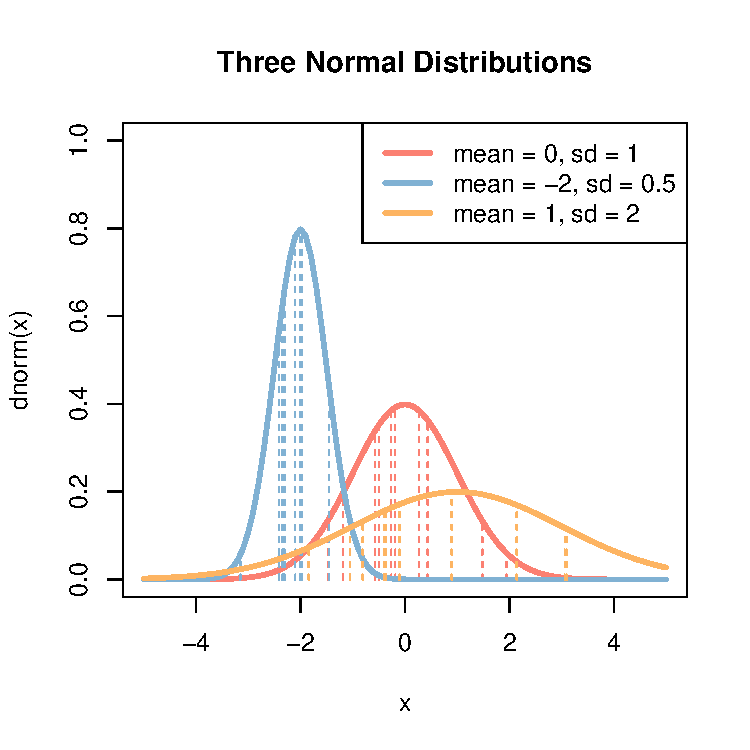
\includegraphics[width=\maxwidth]{figure/unnamed-chunk-54-1} 

\end{knitrout}
\caption{Comparison operators in R}
\label{fig:comparison}
\end{tiny}
\end{marginfigure}



\begin{marginfigure}
\begin{tiny}
\begin{knitrout}
\definecolor{shadecolor}{rgb}{0.969, 0.969, 0.969}\color{fgcolor}\begin{kframe}
\begin{alltt}
\hlcom{# Create blank plot with no margins}
\hlkwd{par}\hlstd{(}\hlkwc{mar} \hlstd{=} \hlkwd{rep}\hlstd{(}\hlnum{0}\hlstd{,} \hlnum{4}\hlstd{))}
\hlkwd{plot}\hlstd{(}\hlnum{1}\hlstd{,} \hlkwc{xlim} \hlstd{=} \hlkwd{c}\hlstd{(}\hlnum{0}\hlstd{,} \hlnum{1}\hlstd{),} \hlkwc{ylim} \hlstd{=} \hlkwd{c}\hlstd{(}\hlnum{0}\hlstd{,} \hlnum{13}\hlstd{),}
     \hlkwc{bty} \hlstd{=} \hlstr{"n"}\hlstd{,} \hlkwc{xlab} \hlstd{=} \hlstr{""}\hlstd{,} \hlkwc{ylab} \hlstd{=} \hlstr{""}\hlstd{,} \hlkwc{main} \hlstd{=} \hlstr{""}\hlstd{,}
     \hlkwc{type} \hlstd{=} \hlstr{"n"}\hlstd{,} \hlkwc{xaxt} \hlstd{=} \hlstr{"n"}\hlstd{,} \hlkwc{yaxt} \hlstd{=} \hlstr{"n"}\hlstd{)}

\hlcom{# Add Main title}
\hlkwd{text}\hlstd{(}\hlnum{.5}\hlstd{,} \hlnum{12.5}\hlstd{,} \hlstr{"log.vec <- data.vec > 0"}\hlstd{,} \hlkwc{cex} \hlstd{=} \hlnum{2}\hlstd{)}

\hlcom{# Data vector}
\hlkwd{text}\hlstd{(}\hlnum{.3}\hlstd{,} \hlnum{11.1}\hlstd{,} \hlstr{"data.vec"}\hlstd{,} \hlkwc{font} \hlstd{=} \hlnum{2}\hlstd{,} \hlkwc{cex} \hlstd{=} \hlnum{1.6}\hlstd{)}
\hlstd{data.vec} \hlkwb{<-} \hlkwd{c}\hlstd{(}\hlnum{2}\hlstd{,} \hlnum{7}\hlstd{,} \hlopt{-}\hlnum{1}\hlstd{,} \hlnum{5}\hlstd{,} \hlopt{-}\hlnum{9}\hlstd{,} \hlopt{-}\hlnum{2}\hlstd{,} \hlnum{3}\hlstd{,} \hlnum{0}\hlstd{,} \hlnum{2}\hlstd{,} \hlopt{-}\hlnum{2}\hlstd{)}
\hlkwd{text}\hlstd{(}\hlkwd{rep}\hlstd{(}\hlnum{.3}\hlstd{,} \hlnum{10}\hlstd{),} \hlnum{10}\hlopt{:}\hlnum{1}\hlstd{, data.vec,} \hlkwc{cex} \hlstd{=} \hlnum{1.6}\hlstd{)}
\hlkwd{rect}\hlstd{(}\hlnum{.25}\hlstd{,} \hlnum{.5}\hlstd{,} \hlnum{.35}\hlstd{,} \hlnum{10.5}\hlstd{)}
\hlkwd{segments}\hlstd{(}\hlkwd{rep}\hlstd{(}\hlnum{.25}\hlstd{,} \hlnum{9}\hlstd{),} \hlkwd{seq}\hlstd{(}\hlnum{1.5}\hlstd{,} \hlnum{9.5}\hlstd{,} \hlnum{1}\hlstd{),}
         \hlkwd{rep}\hlstd{(}\hlnum{.35}\hlstd{,} \hlnum{9}\hlstd{),} \hlkwd{seq}\hlstd{(}\hlnum{1.5}\hlstd{,} \hlnum{9.5}\hlstd{,} \hlnum{1}\hlstd{),} \hlkwc{lty} \hlstd{=} \hlnum{2}\hlstd{)}


\hlcom{# Comparisons}
\hlkwd{text}\hlstd{(}\hlnum{.5}\hlstd{,} \hlnum{11.1}\hlstd{,} \hlstr{"test"}\hlstd{,} \hlkwc{cex} \hlstd{=} \hlnum{1.6}\hlstd{,} \hlkwc{col} \hlstd{=} \hlkwd{gray}\hlstd{(}\hlnum{.5}\hlstd{))}
\hlkwd{text}\hlstd{(}\hlkwd{rep}\hlstd{(}\hlnum{.5}\hlstd{,} \hlnum{10}\hlstd{),} \hlnum{1}\hlopt{:}\hlnum{10}\hlstd{,} \hlstr{"> 0"}\hlstd{,} \hlkwc{col} \hlstd{=} \hlkwd{gray}\hlstd{(}\hlnum{.5}\hlstd{))}

\hlcom{# Logical vector}
\hlkwd{text}\hlstd{(}\hlnum{.7}\hlstd{,} \hlnum{11.1}\hlstd{,} \hlstr{"log.vec"}\hlstd{,} \hlkwc{font} \hlstd{=} \hlnum{2}\hlstd{,} \hlkwc{cex} \hlstd{=} \hlnum{1.6}\hlstd{)}
\hlstd{index.text} \hlkwb{<-} \hlkwd{rep}\hlstd{(}\hlstr{"FALSE"}\hlstd{,} \hlnum{10}\hlstd{)}
\hlstd{index.text[data.vec} \hlopt{>} \hlnum{0}\hlstd{]} \hlkwb{<-} \hlstr{"TRUE"}
\hlstd{col.vec} \hlkwb{<-} \hlkwd{rep}\hlstd{(}\hlstr{"red"}\hlstd{,} \hlnum{10}\hlstd{)}
\hlstd{col.vec[data.vec} \hlopt{>} \hlnum{0}\hlstd{]} \hlkwb{<-} \hlstr{"blue"}
\hlkwd{text}\hlstd{(}\hlkwd{rep}\hlstd{(}\hlnum{.7}\hlstd{,} \hlnum{10}\hlstd{),} \hlnum{10}\hlopt{:}\hlnum{1}\hlstd{,}
     \hlstd{index.text,}
     \hlkwc{col} \hlstd{= col.vec,} \hlkwc{cex} \hlstd{=} \hlnum{1.6}
     \hlstd{)}
\hlkwd{rect}\hlstd{(}\hlnum{.6}\hlstd{,} \hlnum{.7}\hlstd{,} \hlnum{.8}\hlstd{,} \hlnum{10.5}\hlstd{)}
\hlkwd{segments}\hlstd{(}\hlkwd{rep}\hlstd{(}\hlnum{.6}\hlstd{,} \hlnum{9}\hlstd{),} \hlkwd{seq}\hlstd{(}\hlnum{1.5}\hlstd{,} \hlnum{9.5}\hlstd{,} \hlnum{1}\hlstd{),}
         \hlkwd{rep}\hlstd{(}\hlnum{.8}\hlstd{,} \hlnum{9}\hlstd{),} \hlkwd{seq}\hlstd{(}\hlnum{1.5}\hlstd{,} \hlnum{9.5}\hlstd{,} \hlnum{1}\hlstd{),} \hlkwc{lty} \hlstd{=} \hlnum{2}\hlstd{)}
\end{alltt}
\end{kframe}
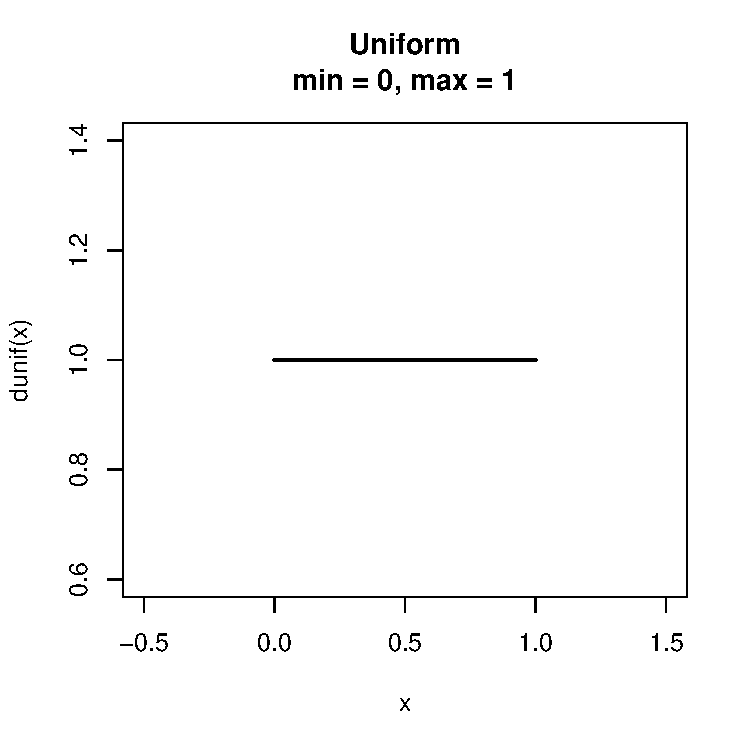
\includegraphics[width=\maxwidth]{figure/unnamed-chunk-55-1} 

\end{knitrout}
\end{tiny}
\label{fig:logvec1}
\caption{Creating a logical vector from a data vector with a comparison operator. In this case, the logical comparison is "> 0" and each element of the data vector is compared to 0.}
\end{marginfigure}

Another way to index data vectors is with logical vectors. A logical vector is a vector that only contains TRUE and FALSE values. If you index a vector with a logical vector (of the same length), you will only receive the values for which the index is TRUE.

You can create a logical vector by using the comparison operators in Figure~\ref{fig:comparison}.

Let's start by creating single scalar logical values so you can see how they work. If you apply a comparison operator to a scalar, R will return a single logical value of TRUE or FALSE. Let's see if 3 truly equals 3 and if 3 is really not greater than 5.

\begin{footnotesize}
\begin{knitrout}
\definecolor{shadecolor}{rgb}{0.969, 0.969, 0.969}\color{fgcolor}\begin{kframe}
\begin{alltt}
\hlnum{3} \hlopt{==} \hlnum{3}
\end{alltt}
\begin{verbatim}
## [1] TRUE
\end{verbatim}
\begin{alltt}
\hlnum{3} \hlopt{>} \hlnum{5}
\end{alltt}
\begin{verbatim}
## [1] FALSE
\end{verbatim}
\end{kframe}
\end{knitrout}
\end{footnotesize}

The negation operator \texttt{!} meaning NOT. To use it, place the statement you are testing in parentheses, and place the \texttt{!} operator before it:

\begin{footnotesize}
\begin{knitrout}
\definecolor{shadecolor}{rgb}{0.969, 0.969, 0.969}\color{fgcolor}\begin{kframe}
\begin{alltt}
\hlstd{pirate} \hlkwb{<-} \hlstr{"david"}
\hlstd{pirate} \hlopt{==} \hlstr{"jack"}
\end{alltt}
\begin{verbatim}
## [1] FALSE
\end{verbatim}
\begin{alltt}
\hlopt{!}\hlstd{(pirate} \hlopt{==} \hlstr{"jack"}\hlstd{)}
\end{alltt}
\begin{verbatim}
## [1] TRUE
\end{verbatim}
\begin{alltt}
\hlopt{!}\hlstd{(}\hlnum{2} \hlopt{==} \hlnum{4}\hlstd{)}
\end{alltt}
\begin{verbatim}
## [1] TRUE
\end{verbatim}
\end{kframe}
\end{knitrout}
\end{footnotesize}




In addition to using single comparison operators, you can combine multiple logical comparisons using the OR \texttt{|} and AND \texttt{\&} commands. The OR command will return TRUE if any of the values in the set is TRUE, while the AND command will only return TRUE if all of the values in the set are TRUE.

\begin{footnotesize}
\begin{knitrout}
\definecolor{shadecolor}{rgb}{0.969, 0.969, 0.969}\color{fgcolor}\begin{kframe}
\begin{alltt}
\hlstd{(}\hlnum{1} \hlopt{<} \hlnum{3}\hlstd{)} \hlcom{# Is 1 less than 3?}
\end{alltt}
\begin{verbatim}
## [1] TRUE
\end{verbatim}
\begin{alltt}
\hlstd{(}\hlnum{4} \hlopt{<} \hlnum{2}\hlstd{)} \hlcom{# Is 4 less than 2?}
\end{alltt}
\begin{verbatim}
## [1] FALSE
\end{verbatim}
\begin{alltt}
\hlstd{(}\hlnum{1} \hlopt{<} \hlnum{3}\hlstd{)} \hlopt{&} \hlstd{(}\hlnum{4} \hlopt{<} \hlnum{2}\hlstd{)} \hlcom{# Is 1 less than 3 and is 4 less than 2?}
\end{alltt}
\begin{verbatim}
## [1] FALSE
\end{verbatim}
\begin{alltt}
\hlstd{(}\hlnum{1} \hlopt{<} \hlnum{3}\hlstd{)} \hlopt{|} \hlstd{(}\hlnum{4} \hlopt{<} \hlnum{2}\hlstd{)} \hlcom{# Is 1 less than 3 OR is 4 less than 2?}
\end{alltt}
\begin{verbatim}
## [1] TRUE
\end{verbatim}
\end{kframe}
\end{knitrout}
\end{footnotesize}

If you apply a comparison operator between a scalar and a vector, R will return a logical vector of length equal to the length of the vector. For example, let's compare a vector of integers from 1 to 10 to a scalar value of three and look at the output:

\begin{footnotesize}
\begin{knitrout}
\definecolor{shadecolor}{rgb}{0.969, 0.969, 0.969}\color{fgcolor}\begin{kframe}
\begin{alltt}
\hlnum{1}\hlopt{:}\hlnum{10} \hlopt{==} \hlnum{3} \hlcom{# Are the values equal to 3?}
\end{alltt}
\begin{verbatim}
##  [1] FALSE FALSE  TRUE FALSE FALSE FALSE FALSE FALSE FALSE FALSE
\end{verbatim}
\end{kframe}
\end{knitrout}
\end{footnotesize}

Let's look at the outputs above: for each value of the object \texttt{vec}, R performs the comparison \texttt{== 3}. Because only the third element of the vector is equal to 3, R returns the value \texttt{FALSE} for all values except the third one.

You can also compare two vectors of equal length and obtain a single logical vector as a result. For example, let's say we have two data vectors (data.1 and data.2) and we want a logical vector telling us which values of the two data vectors are equal. We can do this by just executing \texttt{data.1 == data.2}

\begin{footnotesize}
\begin{knitrout}
\definecolor{shadecolor}{rgb}{0.969, 0.969, 0.969}\color{fgcolor}\begin{kframe}
\begin{alltt}
\hlstd{data.1} \hlkwb{<-} \hlkwd{c}\hlstd{(}\hlnum{1}\hlstd{,} \hlnum{4}\hlstd{,} \hlnum{2}\hlstd{,} \hlnum{3}\hlstd{,} \hlnum{3}\hlstd{)}
\hlstd{data.2} \hlkwb{<-} \hlkwd{c}\hlstd{(}\hlnum{1}\hlstd{,} \hlnum{2}\hlstd{,} \hlnum{4}\hlstd{,} \hlnum{3}\hlstd{,} \hlnum{3}\hlstd{)}
\hlstd{data.1} \hlopt{==} \hlstd{data.2}
\end{alltt}
\begin{verbatim}
## [1]  TRUE FALSE FALSE  TRUE  TRUE
\end{verbatim}
\end{kframe}
\end{knitrout}
\end{footnotesize}

\newfun{x \%in\% y}\index{\%in\%}

One very important function for creating logical indices is \texttt{\%in\%}. This function looks a bit different from other functions because it doesn't follow the typical format of function(x, y). Instead, you place the function \%in\% between its arguments. When you execute x \%in\% y, R will evaluate, for each element in the vector x, if it is in the vector y. For example. Let's create several vectors x and y and use the \%in\% function to text whether or not the elements of x are in y:

\begin{footnotesize}
\begin{knitrout}
\definecolor{shadecolor}{rgb}{0.969, 0.969, 0.969}\color{fgcolor}\begin{kframe}
\begin{alltt}
\hlnum{1} \hlopt \hlkwd{c}\hlstd{(}\hlnum{1}\hlstd{,} \hlnum{2}\hlstd{,} \hlnum{3}\hlstd{,} \hlnum{4}\hlstd{,} \hlnum{5}\hlstd{)}
\end{alltt}
\begin{verbatim}
## [1] TRUE
\end{verbatim}
\end{kframe}
\end{knitrout}
\end{footnotesize}

In this example, R returns a single value of TRUE because it found the value of 1 in the second vector. However, you can also apply the \%in\% function to a vector x that is longer than 1. When you do this, the \%in\% function will return a vector equal to the length of x. Now, let's try an example where we test whether each of several values are in a second set:

\begin{footnotesize}
\begin{knitrout}
\definecolor{shadecolor}{rgb}{0.969, 0.969, 0.969}\color{fgcolor}\begin{kframe}
\begin{alltt}
\hlkwd{c}\hlstd{(}\hlnum{1}\hlstd{,} \hlnum{2}\hlstd{,} \hlnum{3}\hlstd{,} \hlnum{77}\hlstd{,} \hlnum{88}\hlstd{,} \hlnum{99}\hlstd{)} \hlopt \hlkwd{c}\hlstd{(}\hlnum{1}\hlstd{,} \hlnum{2}\hlstd{,} \hlnum{3}\hlstd{,} \hlnum{4}\hlstd{,} \hlnum{5}\hlstd{)}
\end{alltt}
\begin{verbatim}
## [1]  TRUE  TRUE  TRUE FALSE FALSE FALSE
\end{verbatim}
\end{kframe}
\end{knitrout}
\end{footnotesize}

In this example R checked, for each of the values in the first vector if it was in the second vector (\texttt{c(1, 2, 3, 4, 5)}). Because only the first three values (1, 2 and 3) were in the second vector, R returns a vector with 3 TRUE values and 3 FALSE values.

The \%in\% function is very handy for seeing which values in a vector are valid according to a criteria you specify. For example, imagine you conducted a survey where you asked 10 different pirates how many siblings they had and received the following responses:

\begin{knitrout}
\definecolor{shadecolor}{rgb}{0.969, 0.969, 0.969}\color{fgcolor}\begin{kframe}
\begin{alltt}
\hlstd{siblings} \hlkwb{<-} \hlkwd{c}\hlstd{(}\hlnum{3}\hlstd{,} \hlnum{2}\hlstd{,} \hlnum{0}\hlstd{,} \hlopt{-}\hlnum{5}\hlstd{,} \hlnum{0}\hlstd{,} \hlopt{-}\hlnum{20}\hlstd{,} \hlnum{2}\hlstd{,} \hlnum{3}\hlstd{,} \hlnum{1}\hlstd{,} \hlopt{-}\hlnum{200}\hlstd{)}
\end{alltt}
\end{kframe}
\end{knitrout}

Of course, the only valid answers to this question should be 0, 1, 2, ... up to a maximum of say 20; but some of these values appear to be invalid (that is, negative). Let's use the \%in\% function to see which values in the survey are valid. We'll create a vector called \texttt{valid.responses} that represents all possible valid answers to the question (we'll limit the number of siblings to 20). We'll then use \%in\% to create a logical vector indicating which responses were valid. 

\begin{footnotesize}
\begin{knitrout}
\definecolor{shadecolor}{rgb}{0.969, 0.969, 0.969}\color{fgcolor}\begin{kframe}
\begin{alltt}
\hlstd{siblings} \hlkwb{<-} \hlkwd{c}\hlstd{(}\hlnum{3}\hlstd{,} \hlnum{2}\hlstd{,} \hlnum{0}\hlstd{,} \hlopt{-}\hlnum{5}\hlstd{,} \hlnum{0}\hlstd{,} \hlopt{-}\hlnum{20}\hlstd{,} \hlnum{2}\hlstd{,} \hlnum{3}\hlstd{,} \hlnum{1}\hlstd{,} \hlopt{-}\hlnum{200}\hlstd{)}
\hlstd{valid.responses} \hlkwb{<-} \hlkwd{seq}\hlstd{(}\hlnum{0}\hlstd{,} \hlnum{20}\hlstd{,} \hlnum{1}\hlstd{)}
\hlstd{siblings} \hlopt \hlstd{valid.responses}
\end{alltt}
\begin{verbatim}
##  [1]  TRUE  TRUE  TRUE FALSE  TRUE FALSE  TRUE  TRUE  TRUE FALSE
\end{verbatim}
\end{kframe}
\end{knitrout}
\end{footnotesize}

Because the fourth, sixth, and tenth values were not valid (they were negative), the final logical vector gives us FALSE values at those index values, and TRUE values for all others.

\section{Indexing data with logical vectors}

\begin{marginfigure}
\begin{tiny}
\begin{knitrout}
\definecolor{shadecolor}{rgb}{0.969, 0.969, 0.969}\color{fgcolor}\begin{kframe}
\begin{alltt}
\hlcom{# Create blank plot with no margins}
\hlkwd{par}\hlstd{(}\hlkwc{mar} \hlstd{=} \hlkwd{rep}\hlstd{(}\hlnum{0}\hlstd{,} \hlnum{4}\hlstd{))}
\hlkwd{plot}\hlstd{(}\hlnum{1}\hlstd{,} \hlkwc{xlim} \hlstd{=} \hlkwd{c}\hlstd{(}\hlnum{0}\hlstd{,} \hlnum{1}\hlstd{),} \hlkwc{ylim} \hlstd{=} \hlkwd{c}\hlstd{(}\hlnum{0}\hlstd{,} \hlnum{13}\hlstd{),}
     \hlkwc{bty} \hlstd{=} \hlstr{"n"}\hlstd{,} \hlkwc{xlab} \hlstd{=} \hlstr{""}\hlstd{,} \hlkwc{ylab} \hlstd{=} \hlstr{""}\hlstd{,} \hlkwc{main} \hlstd{=} \hlstr{""}\hlstd{,}
     \hlkwc{type} \hlstd{=} \hlstr{"n"}\hlstd{,} \hlkwc{xaxt} \hlstd{=} \hlstr{"n"}\hlstd{,} \hlkwc{yaxt} \hlstd{=} \hlstr{"n"}\hlstd{)}

\hlcom{# Add Main title}
\hlkwd{text}\hlstd{(}\hlnum{.5}\hlstd{,} \hlnum{12.5}\hlstd{,} \hlstr{"output.vec <- data.vec[log.vec]"}\hlstd{,} \hlkwc{cex} \hlstd{=} \hlnum{2}\hlstd{)}

\hlcom{# Data vector}
\hlkwd{text}\hlstd{(}\hlnum{.2}\hlstd{,} \hlnum{11.1}\hlstd{,} \hlstr{"data.vec"}\hlstd{,} \hlkwc{font} \hlstd{=} \hlnum{2}\hlstd{,} \hlkwc{cex} \hlstd{=} \hlnum{1.6}\hlstd{)}
\hlstd{data.vec} \hlkwb{<-} \hlkwd{c}\hlstd{(}\hlnum{2}\hlstd{,} \hlnum{7}\hlstd{,} \hlopt{-}\hlnum{1}\hlstd{,} \hlnum{5}\hlstd{,} \hlopt{-}\hlnum{9}\hlstd{,} \hlopt{-}\hlnum{2}\hlstd{,} \hlnum{3}\hlstd{,} \hlnum{0}\hlstd{,} \hlnum{2}\hlstd{,} \hlopt{-}\hlnum{2}\hlstd{)}
\hlkwd{text}\hlstd{(}\hlkwd{rep}\hlstd{(}\hlnum{.2}\hlstd{,} \hlnum{10}\hlstd{),} \hlnum{10}\hlopt{:}\hlnum{1}\hlstd{, data.vec,} \hlkwc{cex} \hlstd{=} \hlnum{1.6}\hlstd{)}
\hlkwd{rect}\hlstd{(}\hlnum{.15}\hlstd{,} \hlnum{.5}\hlstd{,} \hlnum{.25}\hlstd{,} \hlnum{10.5}\hlstd{)}
\hlkwd{segments}\hlstd{(}\hlkwd{rep}\hlstd{(}\hlnum{.15}\hlstd{,} \hlnum{9}\hlstd{),} \hlkwd{seq}\hlstd{(}\hlnum{1.5}\hlstd{,} \hlnum{9.5}\hlstd{,} \hlnum{1}\hlstd{),}
         \hlkwd{rep}\hlstd{(}\hlnum{.25}\hlstd{,} \hlnum{9}\hlstd{),} \hlkwd{seq}\hlstd{(}\hlnum{1.5}\hlstd{,} \hlnum{9.5}\hlstd{,} \hlnum{1}\hlstd{),} \hlkwc{lty} \hlstd{=} \hlnum{2}\hlstd{)}
\hlkwd{text}\hlstd{(}\hlkwd{rep}\hlstd{(}\hlnum{.12}\hlstd{,} \hlnum{10}\hlstd{),} \hlnum{10}\hlopt{:}\hlnum{1}\hlstd{,} \hlnum{1}\hlopt{:}\hlnum{10}\hlstd{,} \hlkwc{cex} \hlstd{=} \hlnum{.8}\hlstd{)}

\hlcom{# Comparisons}
\hlkwd{text}\hlstd{(}\hlkwd{rep}\hlstd{(}\hlnum{.32}\hlstd{,} \hlnum{10}\hlstd{),} \hlnum{1}\hlopt{:}\hlnum{10}\hlstd{,} \hlstr{"> 0"}\hlstd{,} \hlkwc{col} \hlstd{=} \hlkwd{gray}\hlstd{(}\hlnum{.5}\hlstd{))}

\hlcom{# Logical vector}
\hlkwd{text}\hlstd{(}\hlnum{.5}\hlstd{,} \hlnum{11.1}\hlstd{,} \hlstr{"log.vec"}\hlstd{,} \hlkwc{font} \hlstd{=} \hlnum{2}\hlstd{,} \hlkwc{cex} \hlstd{=} \hlnum{1.6}\hlstd{)}
\hlstd{index.text} \hlkwb{<-} \hlkwd{rep}\hlstd{(}\hlstr{"FALSE"}\hlstd{,} \hlnum{10}\hlstd{)}
\hlstd{index.text[data.vec} \hlopt{>} \hlnum{0}\hlstd{]} \hlkwb{<-} \hlstr{"TRUE"}
\hlstd{col.vec} \hlkwb{<-} \hlkwd{rep}\hlstd{(}\hlstr{"red"}\hlstd{,} \hlnum{10}\hlstd{)}
\hlstd{col.vec[data.vec} \hlopt{>} \hlnum{0}\hlstd{]} \hlkwb{<-} \hlstr{"blue"}
\hlkwd{text}\hlstd{(}\hlkwd{rep}\hlstd{(}\hlnum{.5}\hlstd{,} \hlnum{10}\hlstd{),} \hlnum{10}\hlopt{:}\hlnum{1}\hlstd{,}
     \hlstd{index.text,}
     \hlkwc{col} \hlstd{= col.vec,} \hlkwc{cex} \hlstd{=} \hlnum{1.6}
     \hlstd{)}
\hlkwd{rect}\hlstd{(}\hlnum{.4}\hlstd{,} \hlnum{.5}\hlstd{,} \hlnum{.6}\hlstd{,} \hlnum{10.5}\hlstd{)}
\hlkwd{segments}\hlstd{(}\hlkwd{rep}\hlstd{(}\hlnum{.4}\hlstd{,} \hlnum{9}\hlstd{),} \hlkwd{seq}\hlstd{(}\hlnum{1.5}\hlstd{,} \hlnum{9.5}\hlstd{,} \hlnum{1}\hlstd{),}
         \hlkwd{rep}\hlstd{(}\hlnum{.6}\hlstd{,} \hlnum{9}\hlstd{),} \hlkwd{seq}\hlstd{(}\hlnum{1.5}\hlstd{,} \hlnum{9.5}\hlstd{,} \hlnum{1}\hlstd{),} \hlkwc{lty} \hlstd{=} \hlnum{2}\hlstd{)}

\hlcom{# Output vector}
\hlkwd{text}\hlstd{(}\hlnum{.8}\hlstd{,} \hlnum{11.1}\hlstd{,} \hlstr{"output.vec"}\hlstd{,} \hlkwc{font} \hlstd{=} \hlnum{2}\hlstd{,} \hlkwc{cex} \hlstd{=} \hlnum{1.6}\hlstd{)}
\hlstd{output.text} \hlkwb{<-} \hlstd{data.vec[data.vec} \hlopt{>} \hlnum{0}\hlstd{]}
\hlkwd{text}\hlstd{(}\hlkwd{rep}\hlstd{(}\hlnum{.8}\hlstd{,} \hlnum{5}\hlstd{),} \hlnum{7}\hlopt{:}\hlnum{3}\hlstd{, output.text,} \hlkwc{cex} \hlstd{=} \hlnum{1.6}\hlstd{)}
\hlkwd{rect}\hlstd{(}\hlnum{.75}\hlstd{,} \hlnum{2.5}\hlstd{,} \hlnum{.85}\hlstd{,} \hlnum{7.5}\hlstd{)}
\hlkwd{segments}\hlstd{(}\hlkwd{rep}\hlstd{(}\hlnum{.75}\hlstd{,} \hlnum{9}\hlstd{),} \hlkwd{seq}\hlstd{(}\hlnum{3.5}\hlstd{,} \hlnum{6.5}\hlstd{,} \hlnum{1}\hlstd{),}
         \hlkwd{rep}\hlstd{(}\hlnum{.85}\hlstd{,} \hlnum{9}\hlstd{),} \hlkwd{seq}\hlstd{(}\hlnum{3.5}\hlstd{,} \hlnum{6.5}\hlstd{,} \hlnum{1}\hlstd{),} \hlkwc{lty} \hlstd{=} \hlnum{2}\hlstd{)}
\hlkwd{text}\hlstd{(}\hlkwd{rep}\hlstd{(}\hlnum{.88}\hlstd{,} \hlnum{5}\hlstd{),} \hlnum{7}\hlopt{:}\hlnum{3}\hlstd{,} \hlkwd{which}\hlstd{(data.vec} \hlopt{>} \hlnum{0}\hlstd{),} \hlkwc{cex} \hlstd{=} \hlnum{.8}\hlstd{)}

\hlcom{# Arrows connecting log.vec to output.vec}
\hlkwd{arrows}\hlstd{(}\hlkwd{rep}\hlstd{(}\hlnum{.6}\hlstd{,} \hlnum{5}\hlstd{),}
       \hlnum{11} \hlopt{-} \hlkwd{which}\hlstd{(data.vec} \hlopt{>} \hlnum{0}\hlstd{),}
       \hlkwd{rep}\hlstd{(}\hlnum{.73}\hlstd{,} \hlnum{5}\hlstd{),}
       \hlnum{7}\hlopt{:}\hlnum{3}\hlstd{,} \hlkwc{lwd} \hlstd{=} \hlnum{.5}\hlstd{,} \hlkwc{length} \hlstd{=} \hlnum{.15}
       \hlstd{)}
\end{alltt}
\end{kframe}
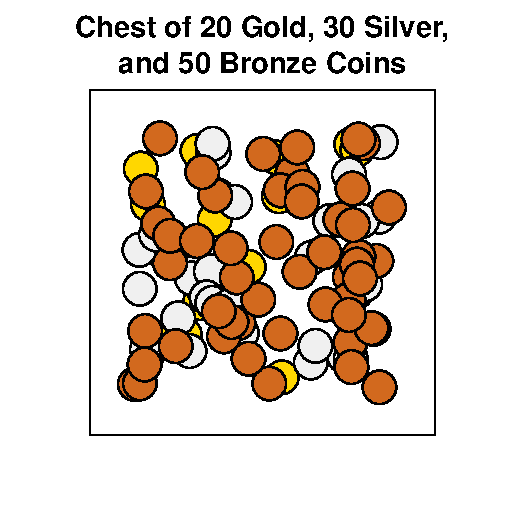
\includegraphics[width=\maxwidth]{figure/unnamed-chunk-65-1} 

\end{knitrout}
\end{tiny}
\label{fig:logvec2}
\caption{A visual representation of how indexing with logical vectors works in R. When you apply a logical vector (a vector containing only TRUE and FALSE values) to a data vector, R will return the the values in the data vector where the logical vector is TRUE.}
\end{marginfigure}

Once we have a logical vector, we can use that vector as an indexing vector. That is, you can use it to select values of a vector that satisfy some criteria you specify. To do this, you create a logical vector containing TRUE and FALSE values. If you then index a data vector (with the same length as the logical vector), R will return the values of the data vector for all TRUE values of the logical vector. See Figure~\ref{fig:logvec2} to see visually how this works.


For example, let's say that we have the following set of data

\begin{footnotesize}
\begin{knitrout}
\definecolor{shadecolor}{rgb}{0.969, 0.969, 0.969}\color{fgcolor}\begin{kframe}
\begin{alltt}
\hlstd{tattoos} \hlkwb{<-} \hlkwd{c}\hlstd{(}\hlnum{4}\hlstd{,} \hlnum{50}\hlstd{,} \hlnum{2}\hlstd{,} \hlnum{39}\hlstd{,} \hlnum{4}\hlstd{,} \hlnum{20}\hlstd{,} \hlnum{4}\hlstd{,} \hlnum{8}\hlstd{,} \hlnum{10}\hlstd{,} \hlnum{100}\hlstd{)}
\end{alltt}
\end{kframe}
\end{knitrout}
\end{footnotesize}

Now, let's say that we want to access just the data points that are less than 10. We'll start by first creating a logical indexing vector that tells us whether each value is less than 1. Then, we'll index the original data vector using this logical vector:

\begin{footnotesize}
\begin{knitrout}
\definecolor{shadecolor}{rgb}{0.969, 0.969, 0.969}\color{fgcolor}\begin{kframe}
\begin{alltt}
\hlstd{log.vec} \hlkwb{<-} \hlstd{tattoos} \hlopt{<} \hlnum{10} \hlcom{# Step 1: Create logical vector}
\hlstd{tattoos[log.vec]} \hlcom{# Step 2: Index the original data by the logical vector}
\end{alltt}
\begin{verbatim}
## [1] 4 2 4 4 8
\end{verbatim}
\end{kframe}
\end{knitrout}
\end{footnotesize}


Logical vectors aren't just good for indexing, you can also use them to figure out which values in a vector satisfy some criteria. To do this, use the function \textt{which()}

\newfun{which(log.vec)}%\marginnote{\texttt{\textbf{which(logical.vector)}}: Tells you the index value of all \texttt{TRUE} values in the logical vector. \\ For example, the command \texttt{which(c(T, T, F))} will return the vector \texttt{[1, 2]}, telling you that the first and second values are true.}

If you apply the function \texttt{which()} to a logical vector, R will tell you which values of the index are TRUE. For example, let's create a logical vector and then see which index values are TRUE

\begin{knitrout}
\definecolor{shadecolor}{rgb}{0.969, 0.969, 0.969}\color{fgcolor}\begin{kframe}
\begin{alltt}
\hlstd{log.vec} \hlkwb{<-} \hlkwd{c}\hlstd{(}\hlnum{TRUE}\hlstd{,} \hlnum{TRUE}\hlstd{,} \hlnum{FALSE}\hlstd{,} \hlnum{TRUE}\hlstd{,} \hlnum{FALSE}\hlstd{)}
\hlkwd{which}\hlstd{(log.vec)}
\end{alltt}
\begin{verbatim}
## [1] 1 2 4
\end{verbatim}
\end{kframe}
\end{knitrout}

By using the \texttt{which()} function, we know that the first, second, and fourth elements of the logical vector are TRUE.

Let's take the example of comparing the treasure chest finding ability of 10 pirates. In each of two years - 2014 and 2015 - I measured how many chests 10 pirates found over the entire year. I recorded these values in two vectors, where the first value of each vector corresponds to the first pirate, and the last value corresponds to the last pirate:

\begin{footnotesize}
\begin{knitrout}
\definecolor{shadecolor}{rgb}{0.969, 0.969, 0.969}\color{fgcolor}\begin{kframe}
\begin{alltt}
\hlstd{pirate.names} \hlkwb{<-} \hlkwd{c}\hlstd{(}\hlstr{"Andrew"}\hlstd{,} \hlstr{"Heidi"}\hlstd{,} \hlstr{"Madisen"}\hlstd{,} \hlstr{"Becki"}\hlstd{,} \hlstr{"Jack Dyanamite"}\hlstd{)}
\hlstd{chests.2014} \hlkwb{<-} \hlkwd{c}\hlstd{(}\hlnum{0}\hlstd{,} \hlnum{10}\hlstd{,} \hlnum{1}\hlstd{,} \hlnum{2}\hlstd{,} \hlnum{5}\hlstd{)}
\hlstd{chests.2015} \hlkwb{<-} \hlkwd{c}\hlstd{(}\hlnum{0}\hlstd{,} \hlnum{6}\hlstd{,} \hlnum{3}\hlstd{,} \hlnum{0}\hlstd{,} \hlnum{20}\hlstd{)}
\end{alltt}
\end{kframe}
\end{knitrout}
\end{footnotesize}

Ok, so let's see which pirates improved their chest findind ability. I'll start by finding the index values where the number of chests found increased between the two years

\begin{footnotesize}
\begin{knitrout}
\definecolor{shadecolor}{rgb}{0.969, 0.969, 0.969}\color{fgcolor}\begin{kframe}
\begin{alltt}
\hlstd{improve.log} \hlkwb{<-} \hlstd{chests.2015} \hlopt{>} \hlstd{chests.2014} \hlcom{# create logical vector}
\hlstd{improve.log} \hlcom{# print values}
\end{alltt}
\begin{verbatim}
## [1] FALSE FALSE  TRUE FALSE  TRUE
\end{verbatim}
\end{kframe}
\end{knitrout}
\end{footnotesize}

If I want to know the index values of the pirates who improved, I can use the \texttt{which()} function. The which function will tell me the index of each TRUE value in a logical vector:

\begin{footnotesize}
\begin{knitrout}
\definecolor{shadecolor}{rgb}{0.969, 0.969, 0.969}\color{fgcolor}\begin{kframe}
\begin{alltt}
\hlkwd{which}\hlstd{(improve.log)}
\end{alltt}
\begin{verbatim}
## [1] 3 5
\end{verbatim}
\end{kframe}
\end{knitrout}
\end{footnotesize}

This vector tells us that the 3rd and 5th pirates found more chests in 2015 than 2014. Now I can use this index value to figure out the names of those pirates:

\begin{footnotesize}
\begin{knitrout}
\definecolor{shadecolor}{rgb}{0.969, 0.969, 0.969}\color{fgcolor}\begin{kframe}
\begin{alltt}
\hlstd{pirate.names[}\hlkwd{which}\hlstd{(improve.log)]}
\end{alltt}
\begin{verbatim}
## [1] "Madisen"        "Jack Dyanamite"
\end{verbatim}
\end{kframe}
\end{knitrout}
\end{footnotesize}


Because you can index vectors with logical vectors, I could get the same results by just indexing \texttt{pirate.names} with \texttt{improve.log}.

\begin{footnotesize}
\begin{knitrout}
\definecolor{shadecolor}{rgb}{0.969, 0.969, 0.969}\color{fgcolor}\begin{kframe}
\begin{alltt}
\hlstd{pirate.names[improve.log]}
\end{alltt}
\begin{verbatim}
## [1] "Madisen"        "Jack Dyanamite"
\end{verbatim}
\end{kframe}
\end{knitrout}
\end{footnotesize}

For this example, the \texttt{which()} command was unnecessary, but it's important to understand the logic of both methods.

\section{Additional helpful vector functions}

Here are some other functions you might find useful when dealing with vectors:


\vspace{5mm} %5mm vertical space
\noindent
\setlength{\fboxrule}{1.5pt}
\fbox{
\parbox{\textwidth}{

\newfun{Other Helpful Vector Functions}

\hline

\begin{description}

\item[\tt{length(x)}] \hfill \\
    The length of a vector
\item[\tt{sort(x)}] \hfill \\
    Sort a vector x. Add the argument \texttt{decreasing = T} to sort in decreasing order.
\item[\tt{rev(x)}] \hfill \\
    Reverse the order of a vector x
\item[\tt{unique(x)}] \hfill \\
    Determine all unique values in a vector x
\item[\tt{table(x)}] \hfill \\
  Determine the number of counts for all unique values in a vector x
  
\end{description}

}
}
\vspace{5mm} %5mm vertical space

Once you have a vector of data, you may want to sort it in order to see, for example, the largest and smallest values. You can do this using the \texttt{sort()} function. Let's look back on my summer joke data and sort the results:

\begin{footnotesize}
\begin{knitrout}
\definecolor{shadecolor}{rgb}{0.969, 0.969, 0.969}\color{fgcolor}\begin{kframe}
\begin{alltt}
\hlstd{tattoos} \hlkwb{<-} \hlkwd{c}\hlstd{(}\hlnum{4}\hlstd{,} \hlnum{50}\hlstd{,} \hlnum{2}\hlstd{,} \hlnum{39}\hlstd{,} \hlnum{4}\hlstd{,} \hlnum{20}\hlstd{,} \hlnum{4}\hlstd{,} \hlnum{8}\hlstd{,} \hlnum{10}\hlstd{,} \hlnum{100}\hlstd{)}
\hlkwd{sort}\hlstd{(tattoos,} \hlkwc{decreasing} \hlstd{= T)} \hlcom{# Sort decreasing}
\end{alltt}
\begin{verbatim}
##  [1] 100  50  39  20  10   8   4   4   4   2
\end{verbatim}
\begin{alltt}
\hlkwd{sort}\hlstd{(tattoos,} \hlkwc{decreasing} \hlstd{= F)} \hlcom{# Sort increasing}
\end{alltt}
\begin{verbatim}
##  [1]   2   4   4   4   8  10  20  39  50 100
\end{verbatim}
\end{kframe}
\end{knitrout}
\end{footnotesize}

You'll notice that the sort function has an argument \texttt{decreasing} which you can set to TRUE or FALSE.

The function \texttt{unique(x)} will tell you all the unique values in the vector, but won't tell you anything about how often each value occurs.

\marginnote{\textbf{unique(x)}: Gives you all unique values in a vector, ignoring the number of times each value occurs.}

\begin{footnotesize}
\begin{knitrout}
\definecolor{shadecolor}{rgb}{0.969, 0.969, 0.969}\color{fgcolor}\begin{kframe}
\begin{alltt}
\hlkwd{unique}\hlstd{(}\hlkwd{c}\hlstd{(}\hlnum{1}\hlstd{,} \hlnum{1}\hlstd{,} \hlnum{2}\hlstd{,} \hlnum{2}\hlstd{,} \hlnum{2}\hlstd{,} \hlnum{4}\hlstd{,} \hlnum{500}\hlstd{))}
\end{alltt}
\begin{verbatim}
## [1]   1   2   4 500
\end{verbatim}
\begin{alltt}
\hlkwd{unique}\hlstd{(}\hlkwd{c}\hlstd{(}\hlstr{"a"}\hlstd{,} \hlstr{"A"}\hlstd{,} \hlstr{"A"}\hlstd{,} \hlstr{"A"}\hlstd{,} \hlstr{"b"}\hlstd{,} \hlstr{"b"}\hlstd{,} \hlstr{"b"}\hlstd{,} \hlstr{"c"}\hlstd{))}
\end{alltt}
\begin{verbatim}
## [1] "a" "A" "b" "c"
\end{verbatim}
\end{kframe}
\end{knitrout}
\end{footnotesize}

The function \texttt{table()} does the same thing as \texttt{unique()}, but goes a step further in telling you how often each of the unique values occurs:

\marginnote{\textbf{table(x)}: Gives you all unique values in a vector and tells you how often each value occurs.}

\begin{footnotesize}
\begin{knitrout}
\definecolor{shadecolor}{rgb}{0.969, 0.969, 0.969}\color{fgcolor}\begin{kframe}
\begin{alltt}
\hlkwd{table}\hlstd{(}\hlkwd{c}\hlstd{(}\hlnum{1}\hlstd{,} \hlnum{1}\hlstd{,} \hlnum{1}\hlstd{,} \hlnum{2}\hlstd{,} \hlnum{2}\hlstd{,} \hlnum{5}\hlstd{,} \hlnum{5}\hlstd{,} \hlnum{700}\hlstd{,} \hlnum{700}\hlstd{,} \hlnum{1000}\hlstd{))}
\end{alltt}
\begin{verbatim}
## 
##    1    2    5  700 1000 
##    3    2    2    2    1
\end{verbatim}
\begin{alltt}
\hlkwd{table}\hlstd{(}\hlkwd{c}\hlstd{(}\hlstr{"a"}\hlstd{,} \hlstr{"A"}\hlstd{,} \hlstr{"A"}\hlstd{,} \hlstr{"A"}\hlstd{,} \hlstr{"b"}\hlstd{,} \hlstr{"b"}\hlstd{,} \hlstr{"b"}\hlstd{,} \hlstr{"c"}\hlstd{))}
\end{alltt}
\begin{verbatim}
## 
## a A b c 
## 1 3 3 1
\end{verbatim}
\end{kframe}
\end{knitrout}
\end{footnotesize}

\section{Set Functions}

R contains many functions that allow you to compare two sets (vectors) of data. See margin Figure~\ref{fig:setfunctions} for a visual depiction. Here are the most common ones:



\vspace{5mm} %5mm vertical space
\noindent
\setlength{\fboxrule}{1.5pt}
\fbox{
\parbox{\textwidth}{

\newfun{Set Functions}

\hline

\begin{description}

\item[\tt{union(x, y)}] \hfill \\
Tells you all unique values included in \textit{either} the vector x or y.
\item[\tt{intersect(x, y)}] \hfill \\
   Tells you all values common in \textit{both} the vectors x and y.
\item[\tt{setdiff(x)}] \hfill \\
    Tells you which values are in the vector x but \textit{not} in the vector y. Keep in mind that \texttt{setdiff(x, y)} is \textit{not} the same as \texttt{setdiff{y, x}}!
\item[\tt{setequal(x)}] \hfill \\
Returns TRUE of the two vectors x and y are identical (ignoring order) and FALSE if they are not identical.
  
\end{description}

}
}
\vspace{5mm} %5mm vertical space



\begin{marginfigure}
\begin{tiny}
\begin{knitrout}
\definecolor{shadecolor}{rgb}{0.969, 0.969, 0.969}\color{fgcolor}\begin{kframe}
\begin{alltt}
\hlkwd{require}\hlstd{(}\hlstr{"plotrix"}\hlstd{)}
\end{alltt}


{\ttfamily\noindent\itshape\color{messagecolor}{\#\# Loading required package: plotrix}}\begin{alltt}
\hlkwd{require}\hlstd{(}\hlstr{"RColorBrewer"}\hlstd{)}

\hlstd{Transparent} \hlkwb{<-} \hlkwa{function}\hlstd{(}\hlkwc{orig.col} \hlstd{=} \hlstr{"red"}\hlstd{,} \hlkwc{trans.val} \hlstd{=} \hlnum{1}\hlstd{,} \hlkwc{maxColorValue} \hlstd{=} \hlnum{255}\hlstd{) \{}

  \hlkwa{if}\hlstd{(}\hlkwd{length}\hlstd{(orig.col)} \hlopt{==} \hlnum{1}\hlstd{) \{orig.col} \hlkwb{<-} \hlkwd{col2rgb}\hlstd{(orig.col)\}}
  \hlkwa{if}\hlstd{(}\hlopt{!}\hlstd{(}\hlkwd{length}\hlstd{(orig.col)} \hlopt \hlkwd{c}\hlstd{(}\hlnum{1}\hlstd{,} \hlnum{3}\hlstd{))) \{}\hlkwd{return}\hlstd{(}\hlkwd{paste}\hlstd{(}\hlstr{"length of original color must be 1 or 3!"}\hlstd{))\}}

  \hlstd{final.col} \hlkwb{<-} \hlkwd{rgb}\hlstd{(orig.col[}\hlnum{1}\hlstd{], orig.col[}\hlnum{2}\hlstd{], orig.col[}\hlnum{3}\hlstd{],} \hlkwc{alpha} \hlstd{= trans.val} \hlopt{*} \hlnum{255}\hlstd{,} \hlkwc{maxColorValue} \hlstd{= maxColorValue)}

  \hlkwd{return}\hlstd{(final.col)}
\hlstd{\}}


\hlstd{color.vec} \hlkwb{<-} \hlkwd{brewer.pal}\hlstd{(}\hlnum{12}\hlstd{,} \hlstr{"Set3"}\hlstd{)}
\hlkwd{par}\hlstd{(}\hlkwc{mar} \hlstd{=} \hlkwd{rep}\hlstd{(}\hlnum{0}\hlstd{,} \hlnum{4}\hlstd{))}
\hlkwd{plot}\hlstd{(}\hlnum{1}\hlstd{,} \hlkwc{xlim} \hlstd{=} \hlkwd{c}\hlstd{(}\hlnum{0}\hlstd{,} \hlnum{1}\hlstd{),} \hlkwc{ylim} \hlstd{=} \hlkwd{c}\hlstd{(}\hlnum{0}\hlstd{,} \hlnum{1}\hlstd{),}
     \hlkwc{bty} \hlstd{=} \hlstr{"n"}\hlstd{,} \hlkwc{xlab} \hlstd{=} \hlstr{""}\hlstd{,} \hlkwc{ylab} \hlstd{=} \hlstr{""}\hlstd{,} \hlkwc{main} \hlstd{=} \hlstr{""}\hlstd{,}
     \hlkwc{type} \hlstd{=} \hlstr{"n"}\hlstd{,} \hlkwc{xaxt} \hlstd{=} \hlstr{"n"}\hlstd{,} \hlkwc{yaxt} \hlstd{=} \hlstr{"n"}\hlstd{)}

\hlkwd{draw.circle}\hlstd{(}\hlkwc{x} \hlstd{=} \hlnum{.35}\hlstd{,} \hlkwc{y} \hlstd{=} \hlnum{.5}\hlstd{,} \hlkwc{radius} \hlstd{=} \hlnum{.35}\hlstd{,} \hlkwc{col} \hlstd{=} \hlkwd{Transparent}\hlstd{(color.vec[}\hlnum{4}\hlstd{],} \hlnum{.3}\hlstd{),} \hlkwc{lwd} \hlstd{=} \hlnum{2}\hlstd{)}
\hlkwd{draw.circle}\hlstd{(}\hlkwc{x} \hlstd{=} \hlnum{.65}\hlstd{,} \hlkwc{y} \hlstd{=} \hlnum{.5}\hlstd{,} \hlkwc{radius} \hlstd{=} \hlnum{.35}\hlstd{,} \hlkwc{col} \hlstd{=} \hlkwd{Transparent}\hlstd{(color.vec[}\hlnum{5}\hlstd{],} \hlnum{.3}\hlstd{),} \hlkwc{lty} \hlstd{=} \hlnum{2}\hlstd{,} \hlkwc{lwd} \hlstd{=} \hlnum{2}\hlstd{)}

\hlkwd{text}\hlstd{(}\hlnum{.35}\hlstd{,} \hlnum{.1}\hlstd{,} \hlstr{"Set X"}\hlstd{,} \hlkwc{cex} \hlstd{=} \hlnum{1.5}\hlstd{)}
\hlkwd{text}\hlstd{(}\hlnum{.65}\hlstd{,} \hlnum{.1}\hlstd{,} \hlstr{"Set Y"}\hlstd{,} \hlkwc{cex} \hlstd{=} \hlnum{1.5}\hlstd{)}

\hlkwd{text}\hlstd{(}\hlnum{.5}\hlstd{,} \hlnum{.5}\hlstd{,} \hlstr{"intersect(x, y)"}\hlstd{)}
\hlkwd{text}\hlstd{(}\hlnum{.15}\hlstd{,} \hlnum{.5}\hlstd{,} \hlstr{"setdiff(x, y)"}\hlstd{)}
\hlkwd{text}\hlstd{(}\hlnum{.85}\hlstd{,} \hlnum{.5}\hlstd{,} \hlstr{"setdiff(y, x)"}\hlstd{)}
\hlkwd{text}\hlstd{(}\hlnum{.5}\hlstd{,} \hlnum{.9}\hlstd{,} \hlstr{"union(x, y)"}\hlstd{)}
\end{alltt}
\end{kframe}
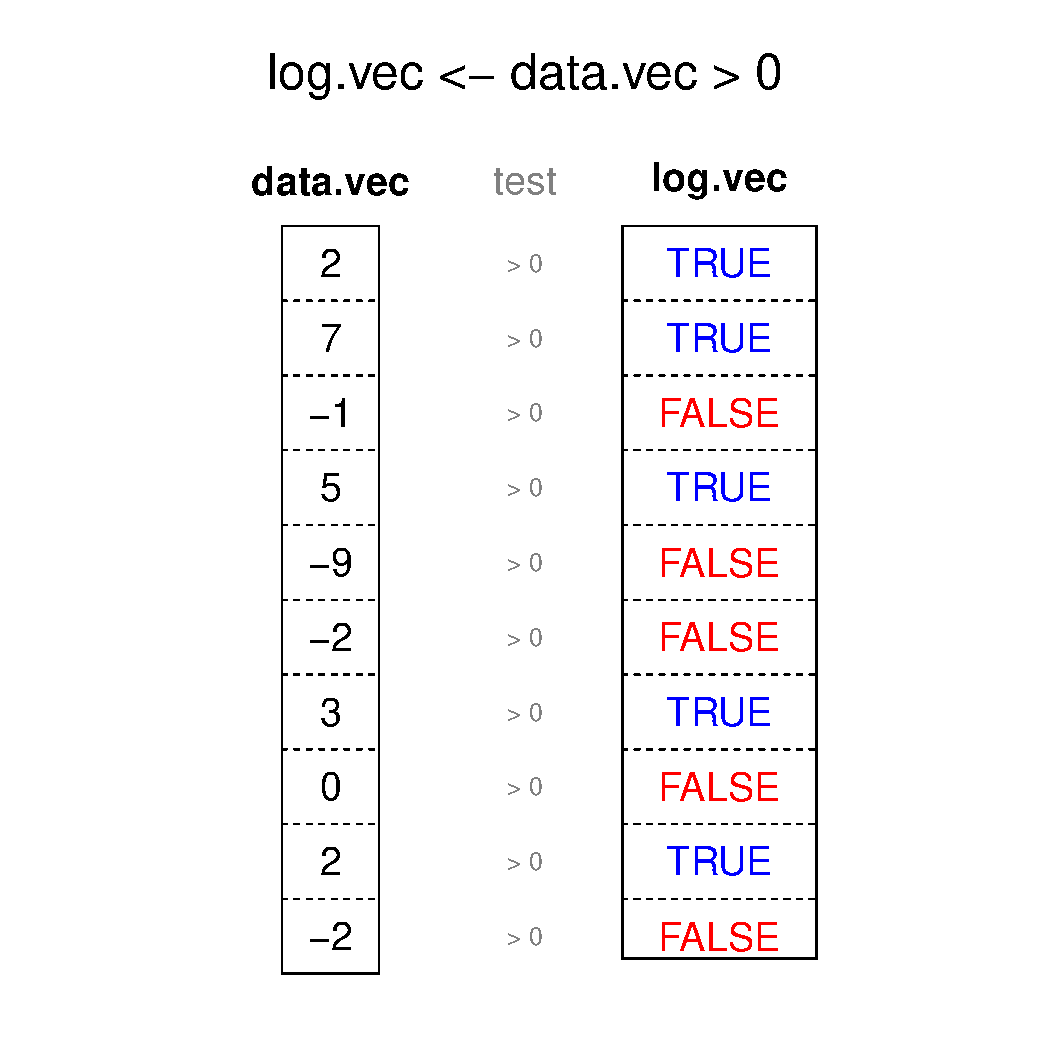
\includegraphics[width=\maxwidth]{figure/unnamed-chunk-77-1} 

\end{knitrout}
\end{tiny}
\label{fig:setfunctions}
\caption{Common set functions in R.}
\end{marginfigure}

\section{Using indexing to remove specific values of a vector}

Sometimes you might want to remove values of a vector before performing some analyses. This might be because some of the values are invalid or just not values that you want to include in your analyses. For example, let's say you asked 7 people how happy they were on a scale of 1 to 5 and received the following responses:

\begin{knitrout}
\definecolor{shadecolor}{rgb}{0.969, 0.969, 0.969}\color{fgcolor}\begin{kframe}
\begin{alltt}
\hlstd{happy} \hlkwb{<-} \hlkwd{c}\hlstd{(}\hlnum{1}\hlstd{,} \hlnum{4}\hlstd{,} \hlnum{2}\hlstd{,} \hlnum{999}\hlstd{,} \hlnum{2}\hlstd{,} \hlnum{3}\hlstd{,} \hlopt{-}\hlnum{2}\hlstd{)}
\end{alltt}
\end{kframe}
\end{knitrout}

As you can see, we have some invalid values (999 and -2) in this vector. We can use logical indexing to create a new vector called \texttt{happy.valid} that only contains values 1 through 5.

\begin{knitrout}
\definecolor{shadecolor}{rgb}{0.969, 0.969, 0.969}\color{fgcolor}\begin{kframe}
\begin{alltt}
\hlstd{valid.log} \hlkwb{<-} \hlstd{happy} \hlopt \hlkwd{c}\hlstd{(}\hlnum{1}\hlstd{,} \hlnum{2}\hlstd{,} \hlnum{3}\hlstd{,} \hlnum{4}\hlstd{,} \hlnum{5}\hlstd{)}
\hlstd{happy.valid} \hlkwb{<-} \hlstd{happy[valid.log]}
\hlstd{happy.valid}
\end{alltt}
\begin{verbatim}
## [1] 1 4 2 2 3
\end{verbatim}
\end{kframe}
\end{knitrout}

As you can see, the new vector \texttt{happy.valid} only contains values from the original vector that are integers from 1 to 5.

R has special functions for testing whether or not values in a dataset are either missing (or infinite). Here are some you can use:
  
  
  
  \vspace{5mm} %5mm vertical space
\noindent
\setlength{\fboxrule}{1.5pt}
\fbox{
\parbox{\textwidth}{

\newfun{Logical testing functions}

\hline

\begin{description}

\item[\tt{is.integer(x)}] \hfill \\
Tests if values in a vector are integers
\item[\tt{is.na(x), is.null(x)}] \hfill \\
Tests if values in a vector are \texttt{NA} or \texttt{NULL}
\item[\tt{is.finite(x)}] \hfill \\
 Tests if a value is a finite numerical value. If a value is NA, NULL, Inf, or -Inf, \texttt{is.finite()} will return \texttt{FALSE}. 
\item[\tt{duplicated(x))}] \hfill \\
Returns \texttt{FALSE} at the first location of each unique value in x, and \texttt{TRUE} for all future locations of unique values. For example, \texttt{duplicated(c(1, 2, 1, 2, 3))} returns \texttt(FALSE, FALSE, TRUE, TRUE, FALSE). If you want to remove duplicated values from a vector, just run \texttt{x <- x[!duplicated(x)]}
  
\end{description}

}
}
\vspace{5mm} %5mm vertical space
  

  
  You can use these functions to generate logical indices for indexing. For example, let's say you had a vector of data with several missing values. To create a new vector of data that does not contain the original NA values, we can index the original \texttt{data} vector with \texttt{is.finite(data)}:
  
\begin{knitrout}
\definecolor{shadecolor}{rgb}{0.969, 0.969, 0.969}\color{fgcolor}\begin{kframe}
\begin{alltt}
\hlstd{data} \hlkwb{<-} \hlkwd{c}\hlstd{(}\hlnum{5}\hlstd{,} \hlnum{2}\hlstd{,} \hlnum{NA}\hlstd{,} \hlnum{3}\hlstd{,} \hlnum{NA}\hlstd{,} \hlnum{10}\hlstd{,} \hlnum{NA}\hlstd{)}
\hlstd{data.finite} \hlkwb{<-} \hlstd{data[}\hlkwd{is.finite}\hlstd{(data)]}
\hlstd{data.finite}
\end{alltt}
\begin{verbatim}
## [1]  5  2  3 10
\end{verbatim}
\end{kframe}
\end{knitrout}


\section{Taking the sum and mean of logical vectors to get counts and percentages}

Many (if not all) R functions that take numeric data as inputs will interpret TRUE values as 1 and FALSE values as 0. This allows us to easily answer questions like "How many values in a data vector are greater than 0?" or "What percentage of values are equal to 5?" by applying the \texttt{sum()} or \texttt{mean()} function to a logical vector.

Let's use this logic to see how many of the integers from 1 to 100 are greater than 0, 50, and 100:

\begin{knitrout}
\definecolor{shadecolor}{rgb}{0.969, 0.969, 0.969}\color{fgcolor}\begin{kframe}
\begin{alltt}
\hlkwd{sum}\hlstd{(}\hlnum{1}\hlopt{:}\hlnum{100} \hlopt{>} \hlnum{0}\hlstd{)} \hlcom{# How many values in 1:100 are greater than 0?}
\end{alltt}
\begin{verbatim}
## [1] 100
\end{verbatim}
\begin{alltt}
\hlkwd{sum}\hlstd{(}\hlnum{1}\hlopt{:}\hlnum{100} \hlopt{>} \hlnum{50}\hlstd{)} \hlcom{# How many values in 1:100 are greater than 50?}
\end{alltt}
\begin{verbatim}
## [1] 50
\end{verbatim}
\begin{alltt}
\hlkwd{sum}\hlstd{(}\hlnum{1}\hlopt{:}\hlnum{100} \hlopt{>} \hlnum{100}\hlstd{)} \hlcom{# How many values in 1:100 are greater than 50?}
\end{alltt}
\begin{verbatim}
## [1] 0
\end{verbatim}
\end{kframe}
\end{knitrout}

These results should make sense: every value from 1:100 is greater than 0, 50 are greater than 50, and non are greater than 100. Now, let's do the same thing but calculate percentages instead of counts using \texttt{mean()} instead of \texttt{sum()}:

\begin{knitrout}
\definecolor{shadecolor}{rgb}{0.969, 0.969, 0.969}\color{fgcolor}\begin{kframe}
\begin{alltt}
\hlkwd{mean}\hlstd{(}\hlnum{1}\hlopt{:}\hlnum{100} \hlopt{>} \hlnum{0}\hlstd{)} \hlcom{# How many values in 1:100 are greater than 0?}
\end{alltt}
\begin{verbatim}
## [1] 1
\end{verbatim}
\begin{alltt}
\hlkwd{mean}\hlstd{(}\hlnum{1}\hlopt{:}\hlnum{100} \hlopt{>} \hlnum{50}\hlstd{)} \hlcom{# How many values in 1:100 are greater than 50?}
\end{alltt}
\begin{verbatim}
## [1] 0.5
\end{verbatim}
\begin{alltt}
\hlkwd{mean}\hlstd{(}\hlnum{1}\hlopt{:}\hlnum{100} \hlopt{>} \hlnum{100}\hlstd{)} \hlcom{# How many values in 1:100 are greater than 50?}
\end{alltt}
\begin{verbatim}
## [1] 0
\end{verbatim}
\end{kframe}
\end{knitrout}

So far so good, now let's try this on our tattoo data:

\begin{knitrout}
\definecolor{shadecolor}{rgb}{0.969, 0.969, 0.969}\color{fgcolor}\begin{kframe}
\begin{alltt}
\hlstd{tattoos} \hlkwb{<-} \hlkwd{c}\hlstd{(}\hlnum{4}\hlstd{,} \hlnum{50}\hlstd{,} \hlnum{2}\hlstd{,} \hlnum{39}\hlstd{,} \hlnum{4}\hlstd{,} \hlnum{20}\hlstd{,} \hlnum{4}\hlstd{,} \hlnum{8}\hlstd{,} \hlnum{10}\hlstd{,} \hlnum{100}\hlstd{)}
\end{alltt}
\end{kframe}
\end{knitrout}

Let's see see how many of these 10 pirates have more than 10 tattoos. We'll do this in two steps; First, we'll create a logical vector indicating which values are greater than 10. Second, we'll take the sum of this logical vector. This will tell us how many \texttt{TRUE} values there are in the logical vector:

\begin{knitrout}
\definecolor{shadecolor}{rgb}{0.969, 0.969, 0.969}\color{fgcolor}\begin{kframe}
\begin{alltt}
\hlstd{log.vec} \hlkwb{<-} \hlstd{tattoos} \hlopt{>} \hlnum{10} \hlcom{# Step 1: Which values are > 10?}
\hlkwd{sum}\hlstd{(log.vec)} \hlcom{# Step 2: How many TRUE values are there?}
\end{alltt}
\begin{verbatim}
## [1] 4
\end{verbatim}
\end{kframe}
\end{knitrout}

Looks like 4 pirates have more than 10 tattoos. Now, let's test what percent of pirates have 5 tattoos or less. We'll do this by first creating the logical vector, and then calculating the \texttt{mean()} of this vector. We can do this because the mean of a vector of 0s and 1s is identical to the percentage of 1s:

\begin{knitrout}
\definecolor{shadecolor}{rgb}{0.969, 0.969, 0.969}\color{fgcolor}\begin{kframe}
\begin{alltt}
\hlstd{log.vec} \hlkwb{<-} \hlstd{tattoos} \hlopt{<=} \hlnum{5} \hlcom{# Step 1: Which values are <= 5?}
\hlkwd{mean}\hlstd{(log.vec)} \hlcom{# Step 2: What percent of values are TRUE?}
\end{alltt}
\begin{verbatim}
## [1] 0.4
\end{verbatim}
\end{kframe}
\end{knitrout}

Looks like 40\% of pirates have 5 tattoos or less.


\marginnote{To see what percentage of values are TRUE in a logical vector, just take the mean of the vector. For example, the command \texttt{mean(c(-1, -2, 1, 1) > 0)} will return \texttt{0.50}, telling you that half of the values are positive.}


\subsection{Additional Tips}

\begin{itemize}

  \item If you have a vector of values and you want to know which values are duplicates of previous values, you can use the \texttt{duplicated} function. This function will go through the vector from beginning to end and tag the first unique instance of a value as TRUE and all repeated instances of a value as FALSE:
  
\begin{knitrout}
\definecolor{shadecolor}{rgb}{0.969, 0.969, 0.969}\color{fgcolor}\begin{kframe}
\begin{alltt}
\hlstd{vec} \hlkwb{<-} \hlkwd{c}\hlstd{(}\hlstr{"a"}\hlstd{,} \hlstr{"b"}\hlstd{,} \hlstr{"a"}\hlstd{,} \hlstr{"a"}\hlstd{,} \hlstr{"c"}\hlstd{)}
\hlkwd{duplicated}\hlstd{(}\hlkwd{c}\hlstd{(}\hlstr{"a"}\hlstd{,} \hlstr{"b"}\hlstd{,} \hlstr{"a"}\hlstd{,} \hlstr{"a"}\hlstd{,} \hlstr{"c"}\hlstd{))}
\end{alltt}
\begin{verbatim}
## [1] FALSE FALSE  TRUE  TRUE FALSE
\end{verbatim}
\end{kframe}
\end{knitrout}

If you want to remove duplicated values from a vector, you can just index the vector by \texttt{!duplicated}:

\begin{knitrout}
\definecolor{shadecolor}{rgb}{0.969, 0.969, 0.969}\color{fgcolor}\begin{kframe}
\begin{alltt}
\hlstd{vec[}\hlopt{!}\hlkwd{duplicated}\hlstd{(vec)]}
\end{alltt}
\begin{verbatim}
## [1] "a" "b" "c"
\end{verbatim}
\end{kframe}
\end{knitrout}

However, you can do the same thing with \texttt{unique()}!

 
\end{itemize}


\section{A worked example - Chicken Weights}

A farmer is testing the effectiveness of three different diets on the weight gain of chickens. When they are born, 50 chicks are randomly assigned to one of 4 diets. Over several time periods, the farmer weighs each chicken. These data are contained in the dataset \texttt{ChickWeight}. Because the data are stored in a dataframe, which we haven't learned yet, we'll convert the four columns in the dataset to vectors as follows:

\begin{knitrout}
\definecolor{shadecolor}{rgb}{0.969, 0.969, 0.969}\color{fgcolor}\begin{kframe}
\begin{alltt}
\hlstd{weights} \hlkwb{<-} \hlstd{ChickWeight}\hlopt{$}\hlstd{weight}
\hlstd{time} \hlkwb{<-} \hlstd{ChickWeight}\hlopt{$}\hlstd{Time}
\hlstd{chick} \hlkwb{<-} \hlkwd{as.numeric}\hlstd{(}\hlkwd{paste}\hlstd{(ChickWeight}\hlopt{$}\hlstd{Chick))}
\hlstd{diet} \hlkwb{<-} \hlkwd{as.numeric}\hlstd{(ChickWeight}\hlopt{$}\hlstd{Diet)}
\end{alltt}
\end{kframe}
\end{knitrout}

Let's answer 5 questions with these vectors:

\begin{enumerate}

  \item What are the first 10 elements of the \texttt{weights} vector and the last 10 elements of the \texttt{weights} vector?\marginnote{To answer the second question, I used the \texttt{length()} function to index index \texttt{weights} to go from 9 elements \textit{before} the end of the vector, to the end of the vector.}
  
\begin{knitrout}
\definecolor{shadecolor}{rgb}{0.969, 0.969, 0.969}\color{fgcolor}\begin{kframe}
\begin{alltt}
\hlstd{weights[}\hlnum{1}\hlopt{:}\hlnum{10}\hlstd{]}
\end{alltt}
\begin{verbatim}
##  [1]  42  51  59  64  76  93 106 125 149 171
\end{verbatim}
\begin{alltt}
\hlstd{weights[(}\hlkwd{length}\hlstd{(weights)} \hlopt{-} \hlnum{9}\hlstd{)}\hlopt{:}\hlkwd{length}\hlstd{(weights)]}
\end{alltt}
\begin{verbatim}
##  [1]  67  84 105 122 155 175 205 234 264 264
\end{verbatim}
\end{kframe}
\end{knitrout}
  
  \item Which chicks were given diets 1 and 2?
  
\begin{knitrout}
\definecolor{shadecolor}{rgb}{0.969, 0.969, 0.969}\color{fgcolor}\begin{kframe}
\begin{alltt}
\hlkwd{unique}\hlstd{(chick[diet} \hlopt{==} \hlnum{1}\hlstd{])}
\end{alltt}
\begin{verbatim}
##  [1]  1  2  3  4  5  6  7  8  9 10 11 12 13 14 15 16 17 18 19 20
\end{verbatim}
\begin{alltt}
\hlkwd{unique}\hlstd{(chick[diet} \hlopt{==} \hlnum{2}\hlstd{])}
\end{alltt}
\begin{verbatim}
##  [1] 21 22 23 24 25 26 27 28 29 30
\end{verbatim}
\end{kframe}
\end{knitrout}

  \item What was the mean weight across all time periods separately for diets 3 and 4?\marginnote{First, I indexed the \texttt{weights} vector with a logical vector created from from \texttt{diet}. I then calculated the mean of this indexed vector.}
  
\begin{knitrout}
\definecolor{shadecolor}{rgb}{0.969, 0.969, 0.969}\color{fgcolor}\begin{kframe}
\begin{alltt}
\hlkwd{mean}\hlstd{(weights[diet} \hlopt{==} \hlnum{3}\hlstd{])}
\end{alltt}
\begin{verbatim}
## [1] 142.95
\end{verbatim}
\begin{alltt}
\hlkwd{mean}\hlstd{(weights[diet} \hlopt{==} \hlnum{4}\hlstd{])}
\end{alltt}
\begin{verbatim}
## [1] 135.2627
\end{verbatim}
\end{kframe}
\end{knitrout}

  \item What was the standard deviation of weights for diets 1 and 2 at time < 10?
  
\begin{knitrout}
\definecolor{shadecolor}{rgb}{0.969, 0.969, 0.969}\color{fgcolor}\begin{kframe}
\begin{alltt}
\hlkwd{sd}\hlstd{(weights[diet} \hlopt{<=} \hlnum{2} \hlopt{&} \hlstd{time} \hlopt{<} \hlnum{10}\hlstd{])}
\end{alltt}
\begin{verbatim}
## [1] 17.2321
\end{verbatim}
\end{kframe}
\end{knitrout}

  \item What was the median weight for chicks 10, 20, and 30 for time periods greater than 10?
  
\begin{knitrout}
\definecolor{shadecolor}{rgb}{0.969, 0.969, 0.969}\color{fgcolor}\begin{kframe}
\begin{alltt}
\hlkwd{median}\hlstd{(weights[chick} \hlopt \hlkwd{c}\hlstd{(}\hlnum{10}\hlstd{,} \hlnum{20}\hlstd{,} \hlnum{30}\hlstd{)} \hlopt{&} \hlstd{time} \hlopt{>} \hlnum{10}\hlstd{])}
\end{alltt}
\begin{verbatim}
## [1] 115
\end{verbatim}
\end{kframe}
\end{knitrout}

  \item Which chicks did not make it until the final time period?\marginnote{This one is a bit tricky. First, I need a vector of all chicks in the study (\texttt{all.chicks}). Next, I need a vector of all chicks that survived to the last time point (\texttt{surviving.chicks}). Third, I need to test, for each chick, whether they are present in the vector of surviving chicks (\texttt{survived.log}). Finally, I index the vector of all chicks where the logical index is FALSE (because we want chicks that did not survive).}

\begin{knitrout}
\definecolor{shadecolor}{rgb}{0.969, 0.969, 0.969}\color{fgcolor}\begin{kframe}
\begin{alltt}
\hlcom{# Step 1: Create a vector of all chicks (all.chicks)}
\hlstd{all.chicks} \hlkwb{<-} \hlkwd{sort}\hlstd{(}\hlkwd{unique}\hlstd{(chick))}

\hlcom{#Step 2: Create a vector of all chicks that survive until the end (surviving.chicks)}
\hlstd{surviving.chicks} \hlkwb{<-} \hlkwd{sort}\hlstd{(}\hlkwd{unique}\hlstd{(chick[time} \hlopt{==} \hlkwd{max}\hlstd{(time)]))}

\hlcom{# Step 3: For each chick, see if it is present in the vector of surviving chicks}
\hlstd{survived.log} \hlkwb{<-} \hlstd{all.chicks} \hlopt \hlstd{surviving.chicks}

\hlcom{# Step 4: Index the vector of all chicks by the logical vector}
\hlstd{all.chicks[survived.log} \hlopt{==} \hlnum{FALSE}\hlstd{]}
\end{alltt}
\begin{verbatim}
## [1]  8 15 16 18 44
\end{verbatim}
\end{kframe}
\end{knitrout}

\end{enumerate}



\end{itemize}

%----------------------------------------------------------------------------------------
%	CHAPTER 5
%----------------------------------------------------------------------------------------

\chapter{5: Matrices and Data Frames}}
\label{ch:5}


Chapter Goals


\begin{enumerate}
  \item Learn about the matrix and dataframe data objects
  \item Create matrices with matrix(), cbind(), and data.frame()
  \item Index matrices/dataframes with brackets [], and \$
  \item Use matrix/dataframe functions dim(), nrow(), ncol(), head(), tail()
  \item Import datasets
\end{enumerate}
 

\section{Creating matrices and dataframes}

By now, you should be comfortable with scalars and vectors. Next, we'll cover the next two most common data objects in R, \textbf{matrices} and \textbf{dataframes}

Matrices and dataframes are both two dimensional objects that contain rows and columns. Really, they're just like spreadsheets in Excel. Each matrix or dataframe contains a certain number of rows (call that number m) and columns (n). You can think of a matrix as a combination of n vectors, where each vector has a length of m. See Figure \ref{fig:scalarvectormatrix} to see the difference.


\begin{marginfigure}
\begin{tiny}
\begin{knitrout}
\definecolor{shadecolor}{rgb}{0.969, 0.969, 0.969}\color{fgcolor}\begin{kframe}
\begin{alltt}
\hlcom{# scalar v vector v matrix}

\hlkwd{par}\hlstd{(}\hlkwc{mar} \hlstd{=} \hlkwd{rep}\hlstd{(}\hlnum{1}\hlstd{,} \hlnum{4}\hlstd{))}
\hlkwd{plot}\hlstd{(}\hlnum{1}\hlstd{,} \hlkwc{xlim} \hlstd{=} \hlkwd{c}\hlstd{(}\hlnum{0}\hlstd{,} \hlnum{10}\hlstd{),} \hlkwc{ylim} \hlstd{=} \hlkwd{c}\hlstd{(}\hlopt{-}\hlnum{.5}\hlstd{,} \hlnum{5}\hlstd{),}
     \hlkwc{xlab} \hlstd{=} \hlstr{""}\hlstd{,} \hlkwc{ylab} \hlstd{=} \hlstr{""}\hlstd{,}
     \hlkwc{xaxt} \hlstd{=} \hlstr{"n"}\hlstd{,} \hlkwc{yaxt} \hlstd{=} \hlstr{"n"}\hlstd{,}
     \hlkwc{bty} \hlstd{=} \hlstr{"n"}\hlstd{,} \hlkwc{type} \hlstd{=} \hlstr{"n"}\hlstd{)}

\hlcom{# scalar}
\hlkwd{rect}\hlstd{(}\hlkwd{rep}\hlstd{(}\hlnum{0}\hlstd{,} \hlnum{1}\hlstd{),} \hlkwd{rep}\hlstd{(}\hlnum{0}\hlstd{,} \hlnum{1}\hlstd{),} \hlkwd{rep}\hlstd{(}\hlnum{1}\hlstd{,} \hlnum{1}\hlstd{),} \hlkwd{rep}\hlstd{(}\hlnum{1}\hlstd{,} \hlnum{1}\hlstd{))}
\hlkwd{text}\hlstd{(}\hlnum{.5}\hlstd{,} \hlopt{-}\hlnum{.5}\hlstd{,} \hlstr{"scalar"}\hlstd{)}

\hlcom{# Vector}
\hlkwd{rect}\hlstd{(}\hlkwd{rep}\hlstd{(}\hlnum{2}\hlstd{,} \hlnum{5}\hlstd{),} \hlnum{0}\hlopt{:}\hlnum{4}\hlstd{,} \hlkwd{rep}\hlstd{(}\hlnum{3}\hlstd{,} \hlnum{5}\hlstd{),} \hlnum{1}\hlopt{:}\hlnum{5}\hlstd{)}
\hlkwd{text}\hlstd{(}\hlnum{2.5}\hlstd{,} \hlopt{-}\hlnum{.5}\hlstd{,} \hlstr{"Vector"}\hlstd{)}

\hlcom{# Matrix}
\hlkwd{rect}\hlstd{(}\hlkwd{rep}\hlstd{(}\hlnum{4}\hlopt{:}\hlnum{8}\hlstd{,} \hlkwc{each} \hlstd{=} \hlnum{5}\hlstd{),}
     \hlkwd{rep}\hlstd{(}\hlnum{0}\hlopt{:}\hlnum{4}\hlstd{,} \hlkwc{times} \hlstd{=} \hlnum{5}\hlstd{),}
     \hlkwd{rep}\hlstd{(}\hlnum{5}\hlopt{:}\hlnum{9}\hlstd{,} \hlkwc{each} \hlstd{=} \hlnum{5}\hlstd{),}
     \hlkwd{rep}\hlstd{(}\hlnum{1}\hlopt{:}\hlnum{5}\hlstd{,} \hlkwc{times} \hlstd{=} \hlnum{5}\hlstd{))}
\hlkwd{text}\hlstd{(}\hlnum{6.5}\hlstd{,} \hlopt{-}\hlnum{.5}\hlstd{,} \hlstr{"Matrix / Data Frame"}
     \hlstd{)}
\end{alltt}
\end{kframe}
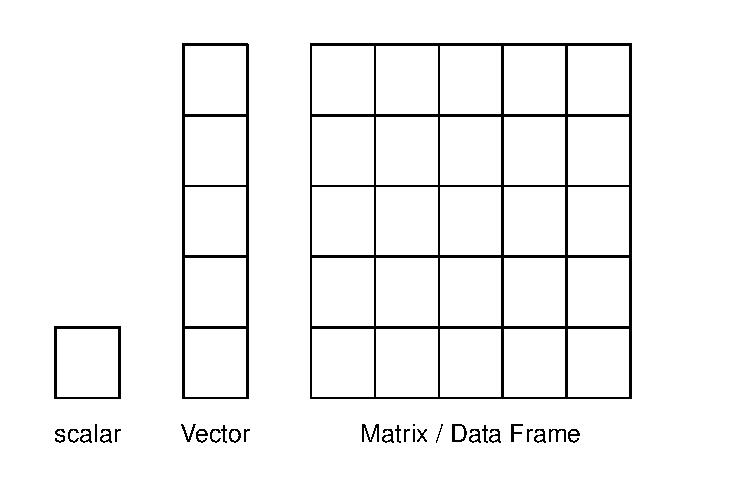
\includegraphics[width=\maxwidth]{figure/unnamed-chunk-95-1} 

\end{knitrout}
\caption{scalar, Vector, Matrix... ::drops mike::}
\label{fig:scalarvectormatrix}
\end{tiny}
\end{marginfigure}

You can use several functions in R to create matrices and dataframes. In the next sections we'll cover the most common ones.

\subsection{cbind() and rbind()}

\texttt{cbind()} and \texttt{rbind()} both create matrices by combining several vectors together into a single matrix. cbind() combines vectors as columns in the matrix, while rbind() combines them as rows.



\vspace{5mm} %5mm vertical space
\noindent
\setlength{\fboxrule}{1.5pt}
\fbox{
\parbox{\textwidth}{

\newfun{cbind(), rbind()}\index{cbind()}\index{rbind()}

\hline

\begin{description}

  \item[\tt{x, y, ...}] \hfill \\
      One or more vectors to be combined into a matrix
\end{description}

}
}
\vspace{5mm} %5mm vertical space

Let's use these functions to create a matrix with the numbers 1 through 30. First, we'll create three vectors of length 10, then we'll combine them into one matrix.

\begin{footnotesize}
\begin{knitrout}
\definecolor{shadecolor}{rgb}{0.969, 0.969, 0.969}\color{fgcolor}\begin{kframe}
\begin{alltt}
\hlstd{x} \hlkwb{<-} \hlnum{1}\hlopt{:}\hlnum{10}
\hlstd{y} \hlkwb{<-} \hlnum{11}\hlopt{:}\hlnum{20}
\hlstd{z} \hlkwb{<-} \hlnum{21}\hlopt{:}\hlnum{30}

\hlstd{matrix.1} \hlkwb{<-} \hlkwd{rbind}\hlstd{(x, y, z)}
\hlstd{matrix.1}
\end{alltt}
\begin{verbatim}
##   [,1] [,2] [,3] [,4] [,5] [,6] [,7] [,8] [,9] [,10]
## x    1    2    3    4    5    6    7    8    9    10
## y   11   12   13   14   15   16   17   18   19    20
## z   21   22   23   24   25   26   27   28   29    30
\end{verbatim}
\begin{alltt}
\hlstd{matrix.2} \hlkwb{<-} \hlkwd{cbind}\hlstd{(x, y, z)}
\hlstd{matrix.2}
\end{alltt}
\begin{verbatim}
##        x  y  z
##  [1,]  1 11 21
##  [2,]  2 12 22
##  [3,]  3 13 23
##  [4,]  4 14 24
##  [5,]  5 15 25
##  [6,]  6 16 26
##  [7,]  7 17 27
##  [8,]  8 18 28
##  [9,]  9 19 29
## [10,] 10 20 30
\end{verbatim}
\end{kframe}
\end{knitrout}
\end{footnotesize}

As you can see, the \texttt{rbind()} function combined the vectors as rows in the final matrix, while the \texttt{cbind()} function combined them as columns.

If you want to create a matrix from a single vector of data, you can do this using the \texttt{matrix()} function.


\vspace{5mm} %5mm vertical space
\noindent
\setlength{\fboxrule}{1.5pt}
\fbox{
\parbox{\textwidth}{

\newfun{matrix()}\index{matrix()}

\hline

\begin{description}

  \item[\tt{data}] \hfill \\
      A vector of data
        \item[\tt{nrow}] \hfill \\
      The number of rows in the final matrix
        \item[\tt{ncol}] \hfill \\
      The number of columns in the final matrix
        \item[\tt{byrow}] \hfill \\
      A logical value indicating whether to fill the matrix by row or column
\end{description}

}
}
\vspace{5mm} %5mm vertical space


Let's use the \texttt{matrix()} function to re-create a matrix containing the values from 1 to 30.

\begin{footnotesize}
\begin{knitrout}
\definecolor{shadecolor}{rgb}{0.969, 0.969, 0.969}\color{fgcolor}\begin{kframe}
\begin{alltt}
\hlstd{matrix.1} \hlkwb{<-} \hlkwd{matrix}\hlstd{(}\hlkwc{data} \hlstd{=} \hlnum{1}\hlopt{:}\hlnum{30}\hlstd{,}
                   \hlkwc{nrow} \hlstd{=} \hlnum{10}\hlstd{,}
                   \hlkwc{ncol} \hlstd{=} \hlnum{3}\hlstd{)}
\hlstd{matrix.1}
\end{alltt}
\begin{verbatim}
##       [,1] [,2] [,3]
##  [1,]    1   11   21
##  [2,]    2   12   22
##  [3,]    3   13   23
##  [4,]    4   14   24
##  [5,]    5   15   25
##  [6,]    6   16   26
##  [7,]    7   17   27
##  [8,]    8   18   28
##  [9,]    9   19   29
## [10,]   10   20   30
\end{verbatim}
\begin{alltt}
\hlstd{matrix.2} \hlkwb{<-} \hlkwd{matrix}\hlstd{(}\hlkwc{data} \hlstd{=} \hlnum{1}\hlopt{:}\hlnum{30}\hlstd{,}
                   \hlkwc{nrow} \hlstd{=} \hlnum{3}\hlstd{,}
                   \hlkwc{ncol} \hlstd{=} \hlnum{10}\hlstd{)}
\hlstd{matrix.2}
\end{alltt}
\begin{verbatim}
##      [,1] [,2] [,3] [,4] [,5] [,6] [,7] [,8] [,9] [,10]
## [1,]    1    4    7   10   13   16   19   22   25    28
## [2,]    2    5    8   11   14   17   20   23   26    29
## [3,]    3    6    9   12   15   18   21   24   27    30
\end{verbatim}
\end{kframe}
\end{knitrout}
\end{footnotesize}

Keep in mind that matrices can either contain numbers or characters. If you try to create a matrix with both numbers and characters, it will turn all the numbers into characters:

\begin{footnotesize}
\begin{knitrout}
\definecolor{shadecolor}{rgb}{0.969, 0.969, 0.969}\color{fgcolor}\begin{kframe}
\begin{alltt}
\hlkwd{cbind}\hlstd{(}\hlnum{1}\hlopt{:}\hlnum{5}\hlstd{,} \hlkwd{c}\hlstd{(}\hlstr{"a"}\hlstd{,} \hlstr{"b"}\hlstd{,} \hlstr{"c"}\hlstd{,} \hlstr{"d"}\hlstd{,} \hlstr{"e"}\hlstd{))}
\end{alltt}
\begin{verbatim}
##      [,1] [,2]
## [1,] "1"  "a" 
## [2,] "2"  "b" 
## [3,] "3"  "c" 
## [4,] "4"  "d" 
## [5,] "5"  "e"
\end{verbatim}
\end{kframe}
\end{knitrout}
\end{footnotesize}

\subsection{Dataframe: An m x n object containing numbers, strings and factors}

A dataframe looks a lot like a matrix at first: it is also rectangular and has m rows and n columns. However, unlike matrices, dataframes can contain *both* string vectors and numeric vectors within the same object. For this reason, most large datasets in R, for example, a survey including numeric data and text data, will be stored as dataframes.

\marginnote{A dataframe is just a more flexible matrix that allows you to combine both character and numeric vectors into the same data object. Because dataframes are more flexible than matrices, Most datafiles you use will be stored as dataframes.}

\newfun{data.frame()}\index{data.frame()}

To create a dataframe, you can use the \texttt{data.frame()} function. Let's create a dataframe of fictional survey data. I'll create 5 entries for Males and 5 entries for Females. I'll then generate 10 heights from a normal distribution with mean 150 and standard deviation 10.

\begin{footnotesize}
\begin{knitrout}
\definecolor{shadecolor}{rgb}{0.969, 0.969, 0.969}\color{fgcolor}\begin{kframe}
\begin{alltt}
\hlstd{survey} \hlkwb{<-} \hlkwd{data.frame}\hlstd{(}\hlstr{"gender"} \hlstd{=} \hlkwd{rep}\hlstd{(}\hlkwd{c}\hlstd{(}\hlstr{"Female"}\hlstd{,} \hlstr{"Male"}\hlstd{),} \hlkwc{each} \hlstd{=} \hlnum{10}\hlstd{),}
                     \hlstr{"height"} \hlstd{=} \hlkwd{rnorm}\hlstd{(}\hlnum{20}\hlstd{,} \hlkwc{mean} \hlstd{=} \hlnum{150}\hlstd{,} \hlkwc{sd} \hlstd{=} \hlnum{10}\hlstd{),}
                     \hlkwc{stringsAsFactors} \hlstd{= F} \hlcom{# don't convert strings to factors}
                    \hlstd{)}
\hlstd{survey} \hlcom{# Print the dataframe}
\end{alltt}
\begin{verbatim}
##    gender   height
## 1  Female 157.3150
## 2  Female 155.3883
## 3  Female 144.3909
## 4  Female 145.0709
## 5  Female 155.6452
## 6  Female 149.5139
## 7  Female 154.8151
## 8  Female 137.8721
## 9  Female 146.3488
## 10 Female 135.1628
## 11   Male 163.7332
## 12   Male 149.0106
## 13   Male 138.2191
## 14   Male 140.5986
## 15   Male 153.2361
## 16   Male 151.7072
## 17   Male 151.0853
## 18   Male 160.3671
## 19   Male 143.5117
## 20   Male 143.4082
\end{verbatim}
\end{kframe}
\end{knitrout}
\end{footnotesize}

You'll notice I included the argument \texttt{stringsAsFactors = F}, this tells R to NOT convert the strings (the Gender column) to a factor datatype. For now, don't worry about what factors are. Just know that you don't want to use them just yet!

\section{Data sets pre-loaded in R}

Until now, we've used the functions \texttt{matrix()} and \texttt{dataframe()} to manually create our own datasets within R. However, for demonstration purposes, it's frequently easier to use existing datasets. Thankfully, R has us covered: R has several datasets that come pre-installed in a package called \texttt{datasets}. While you probably won't make any major scientific discoveries with these datasets, they allow all R users to test and compare code on the same sets of data.\marginnote{To see a complete list of all the datasets included in the \texttt{datasets} package, run the code: \texttt{library(help = "datasets")}} Here are a few datasets that we will be using in future examples:

\begin{itemize}
  \item \texttt{ChickWeight}: Weight versus age of chicks on four different diets
  \item \texttt{InsectSprays}: Effectiveness of six different types of insect sprays
  \item \texttt{ToothGrowth}: The effects of different levels of vitamin C on the tooth growth of guinea pigs.
\end{itemize}

Since these datasets are preloaded in R, you can always access them by by name. We'll use them in the following examples.

\section{Viewing matrices and dataframes}

When you start working with a new dataset loaded as a matrix or dataframe, you'll usually want to get a quick visual look at it to make sure it looks ok. There are two functions that I use to do this:

\newfun{head(x)}\index{head()}

The function \texttt{head(x)} will show you the first few rows of a matrix / dataframe. Personally, I am constantly using this function to make sure that I didn't screw up a dataset when I'm working on it. Let's look at the first few rows of the dataframe \texttt{ChickWeight}, which contains data on the growth of chickens on several different diets.

\begin{knitrout}
\definecolor{shadecolor}{rgb}{0.969, 0.969, 0.969}\color{fgcolor}\begin{kframe}
\begin{alltt}
\hlkwd{head}\hlstd{(ChickWeight)}
\end{alltt}
\begin{verbatim}
##   weight Time Chick Diet
## 1     42    0     1    1
## 2     51    2     1    1
## 3     59    4     1    1
## 4     64    6     1    1
## 5     76    8     1    1
## 6     93   10     1    1
\end{verbatim}
\end{kframe}
\end{knitrout}

The \texttt{head()} function only shows you the first few rows of a dataframe, but usually this is enough to get a visual sense of the names of the dataframe, the number of columns, and the type of data in each column. But what if you want to see all values? You could print the entire dataframe into the console, but the console isn't a very friendly environment to view data. Instead, you can use the \texttt{View()} function, which will print the entire dataframe into a spreadsheet-like window:

\newfun{View(x)}\index{View()}

Let's use the \texttt{View()} function to look at the entire \texttt{ToothGrowth} dataframe:

\begin{knitrout}
\definecolor{shadecolor}{rgb}{0.969, 0.969, 0.969}\color{fgcolor}\begin{kframe}
\begin{alltt}
\hlkwd{View}\hlstd{(ToothGrowth)}
\end{alltt}
\end{kframe}
\end{knitrout}

When you run this code, you should see a separate window open (see Figure~\ref{fig:toothgrowthscreenshot}). You can use this window to scroll through the data, sort it via column values (by clicking on the column name), and even apply filters using the filter button on the top left of the screen. However, keep in mind that anything you do in the \texttt{View()} window will \textit{not} change the actual dataframe in any way. You cannot add or remove data using the window, and any sorting or filtering you apply won't be replicated in the actual data.

\begin{figure}[h]
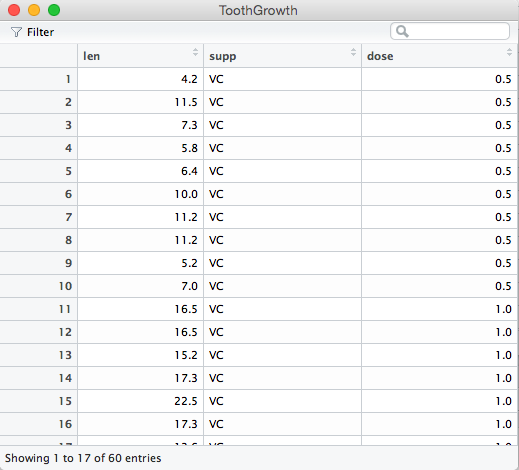
\includegraphics[width=10cm,keepaspectration]{/Users/Nathaniel/Dropbox/Git/YaRrr_Book/media/toothgrowthscreenshot.png}
\label{fig:toothgrowthscreenshot}
\caption{Screenshot of the window from \texttt{View(ToothGrowth)}. You can use this window to visually sort and filter the data to get an idea of how it looks, but you can't add or remove data and nothing you do will actually change the dataframe.}
\end{figure}

\section{Loading data into R with read.table()}

So far we've used either randomly generated data, or datasets pre-loaded in R. But how do you get an existing dataset into R? For the most part, getting datasets into R isn't that tricky - but only if your data is already in a 'nice' format. By 'nice,' I mean a text file with tab (or comma) separated columns. If your data is in another format (like Excel or Shitty Piece of Shitty Shit), I strongly recommend first exporting the data to a tab-delimited text file, and only then loading the data into R. That said, if for some reason you absolutely have to load a non-text file into R, look at the \textit{Additional Tips} sections for instructions.\marginnote{Import data into R as comma or tab-delimited text files whenever possible. If you need to load data in another format (e.g.; Excel), save it as a text file from the original program first.}

Once you have a text file, you can load it into R using the \texttt{read.table()} function. To use the \texttt{read.table()} function, you need to know where the text file is located on your computer. To do this, find the file on your harddrive then right-click it and view its properties. You should be able to see its file-path there. For example, the file path of a text file called \texttt{mydata} on my desktop is \texttt{"Users/Nathaniel/Desktop/mydata.txt"}.

Here are the main arguments to \texttt{read.table()} (to see all of them, run \texttt{?read.table})



\vspace{5mm} %5mm vertical space
\noindent
\setlength{\fboxrule}{1.5pt}
\fbox{
\parbox{\textwidth}{

\newfun{read.table()}\index{readltab.e()}

\hline

\begin{description}

  \item[\tt{file}] \hfill \\
      The document's file path (make sure to enter as a string with quotation marks!) OR an html link to a file.
        \item[\tt{header}] \hfill \\
      A logical value indicating whether the data has a header row or not.
        \item[\tt{ncol}] \hfill \\
      The number of columns in the final matrix
        \item[\tt{sep}] \hfill \\
      A string indicating how the columns are separated. For comma separated files, use \texttt{","}, for tab-delimited files, use \texttt{"\textbackslash t"}
      \item[\tt{stringsAsFactors}] \hfill \\
     A logical value indicating whether or not to convert strings to factors. I always set this to FALSE (because I don't like using factors)
\end{description}

}
}
\vspace{5mm} %5mm vertical space


To test this function, let's read in the datafile called \texttt{Flights.txt}. This dataset contains data on all flights leaving the Houston airport in 2011. You can access this data in one of two ways: First, you can download this file from: http://nathanieldphillips.com/wp-content/uploads/2015/04/Flights.txt) and a note of its directory on your computer (on my computer, the path is \texttt{/Users/Nathaniel/Dropbox/Public/Flights.txt}). You can then load the data into R by using \texttt{read.table}:

\begin{footnotesize}
\begin{knitrout}
\definecolor{shadecolor}{rgb}{0.969, 0.969, 0.969}\color{fgcolor}\begin{kframe}
\begin{alltt}
\hlstd{Flights} \hlkwb{<-} \hlkwd{read.table}\hlstd{(}\hlkwc{file} \hlstd{=} \hlstr{"/Users/Nathaniel/Dropbox/Public/Flights.txt"}\hlstd{,}
                      \hlkwc{header} \hlstd{= T,}
                      \hlkwc{sep} \hlstd{=} \hlstr{"\textbackslash{}t"}\hlstd{,} \hlcom{# tab-delimited}
                      \hlkwc{stringsAsFactors} \hlstd{= F}
                      \hlstd{)}
\end{alltt}
\end{kframe}
\end{knitrout}
\end{footnotesize}

If you receive an error, it's probably because you entered the file path incorrectly. One trick to get the file path easily is by using RStudio's \textbf{Import Dataset} menu (see \textit{Additional Tips}). If you got the directory location correct, and the file exists, then you should not receive any error warning after executing \texttt{read.table()}.

Alternatively, you can load the dataset directly into R by entering the HTML link as the \texttt{file} argument to \texttt{read.table}

\begin{footnotesize}
\begin{knitrout}
\definecolor{shadecolor}{rgb}{0.969, 0.969, 0.969}\color{fgcolor}\begin{kframe}
\begin{alltt}
\hlstd{Flights} \hlkwb{<-} \hlkwd{read.table}\hlstd{(}\hlkwc{file} \hlstd{=} \hlstr{"http://nathanieldphillips.com/wp-content/uploads/2015/04/Flights.txt"}\hlstd{,}
                      \hlkwc{header} \hlstd{= T,}
                      \hlkwc{sep} \hlstd{=} \hlstr{"\textbackslash{}t"}\hlstd{,} \hlcom{# tab-delimited}
                      \hlkwc{stringsAsFactors} \hlstd{= F}
                      \hlstd{)}
\end{alltt}
\end{kframe}
\end{knitrout}
\end{footnotesize}

The data is now stored as a dataframe and you can now access it via the object name you assigned it to (in my case, I called it \texttt{Flights}). To make sure it loaded correctly, try seeing the first few rows with \texttt{head()}

\begin{footnotesize}
\begin{knitrout}
\definecolor{shadecolor}{rgb}{0.969, 0.969, 0.969}\color{fgcolor}\begin{kframe}
\begin{alltt}
\hlkwd{head}\hlstd{(Flights)}
\end{alltt}
\begin{verbatim}
##                  date hour minute  dep  arr dep_delay arr_delay carrier
## 1 2011-01-01 12:00:00   14      0 1400 1500         0       -10      AA
## 2 2011-01-02 12:00:00   14      1 1401 1501         1        -9      AA
## 3 2011-01-03 12:00:00   13     52 1352 1502        -8        -8      AA
## 4 2011-01-04 12:00:00   14      3 1403 1513         3         3      AA
## 5 2011-01-05 12:00:00   14      5 1405 1507         5        -3      AA
## 6 2011-01-06 12:00:00   13     59 1359 1503        -1        -7      AA
##   flight dest  plane cancelled time dist
## 1    428  DFW N576AA         0   40  224
## 2    428  DFW N557AA         0   45  224
## 3    428  DFW N541AA         0   48  224
## 4    428  DFW N403AA         0   39  224
## 5    428  DFW N492AA         0   44  224
## 6    428  DFW N262AA         0   45  224
\end{verbatim}
\end{kframe}
\end{knitrout}
\end{footnotesize}

\subsection{Additional tips}

\begin{itemize}
  \item If you're like me, and you hate figuring out (and typing) the directory of a file, you can use RStudio's menu to help you. If you click on the Environment window and click the button \texttt{Import Dataset}, you'll activate a menu that will allow you to select the file using your computer's finder. You'll then be greeted with a graphical interface for setting the import parameters. When you are finished, RStudio not only import the dataset, but it will paste the R code needed to import the data into the console. You can then copy the code (which includes the file path) and paste it into your R document so the next time you use the document you can just run the code to import the data.
  \item There are many functions other than \texttt{read.table()} for importing data. For example, the functions \texttt{read.csv} and \texttt{read.delim} are specific for importing comma-separated and tab-separated text files. In practice, these functions do the same thing as \texttt{read.table}, but they don't require you to specify a \texttt{sep} argument. Personally, I always use \texttt{read.table()} because it always works and I don't like trying to remember unnecessary functions.
  \item If you absolutely have to read a non-text file into R, check out the package called \texttt{foreign}. This package has functions for importing Stata, SAS and Shitty Piece of Shitty Shit files directly into R. To read Excel files, try the package \texttt{xlsx}

\end{itemize}

%----------------------------------------------------------------------------------------
%	CHAPTER 6
%----------------------------------------------------------------------------------------

\chapter{6: Basic Dataframe Manipulation}
\label{ch:6}


Chapter Goals

\begin{enumerate}
  \item Getting basic information about dataframes: dim(), nrow(), ncol(), summary()
  \item Indexing dataframes with brackets [,], and \$
  \item Subsettting dataframes with logical indexing and subset()
  \item Recoding values in a dataframe with indexing
\end{enumerate}

In this chapter we'll cover how to do some basic analyses on dataframes. We'll focus on dataframes, and not on matrices, because most datasets you use will be stored as dataframes. However, if you do find yourself working with matrices, many of the techniques you'll learn in this chapter will also apply to them.


\section{Getting information about matrices and dataframes}

When you are working with dataframes, you will frequently want to know its general attributes, such as the number of rows and columns it has. Here are some common functions to get basic information about a dataframe:

\begin{itemize}
  \item dim(x): Number of rows and columns in a dataframe x (returns a vector of length 2)
  \item nrow(x) ncol(x): How many rows or columns are there in a dataframe x (each function returns a scalar)
  \item summary(x): Summary of information about each column in a dataframe x
\end{itemize}


\begin{footnotesize}
\begin{knitrout}
\definecolor{shadecolor}{rgb}{0.969, 0.969, 0.969}\color{fgcolor}\begin{kframe}
\begin{alltt}
\hlkwd{dim}\hlstd{(survey)} \hlcom{# How many rows and columns?}
\end{alltt}
\begin{verbatim}
## [1] 20  2
\end{verbatim}
\begin{alltt}
\hlkwd{nrow}\hlstd{(survey)} \hlcom{# How many rows?}
\end{alltt}
\begin{verbatim}
## [1] 20
\end{verbatim}
\begin{alltt}
\hlkwd{ncol}\hlstd{(survey)} \hlcom{# How many columns?}
\end{alltt}
\begin{verbatim}
## [1] 2
\end{verbatim}
\begin{alltt}
\hlkwd{summary}\hlstd{(survey)} \hlcom{# Summary information on each column}
\end{alltt}
\begin{verbatim}
##     gender              height     
##  Length:20          Min.   :135.2  
##  Class :character   1st Qu.:143.5  
##  Mode  :character   Median :149.3  
##                     Mean   :148.8  
##                     3rd Qu.:155.0  
##                     Max.   :163.7
\end{verbatim}
\end{kframe}
\end{knitrout}
\end{footnotesize}

While you might not see the benefits of these functions now, they will become invaluable later if you conduct simulations on datasets.

Next let's start with the basics of indexing dataframes using brackets.

\section{Indexing dataframes with brackets [rows, columns]}

Just like vectors, you can access specific data in dataframes using brackets. But now, instead of just using one indexing vector, we use two indexing vectors: one for the rows and one for the columns. To do this, use the notation \texttt{data[rows, columns]}, where \texttt{rows} and \texttt{columns} are scalars or vectors of the row and column numbers you want to get.

Let's try this on the \texttt{ChickWeight} dataframe that comes with R.

\begin{marginfigure}
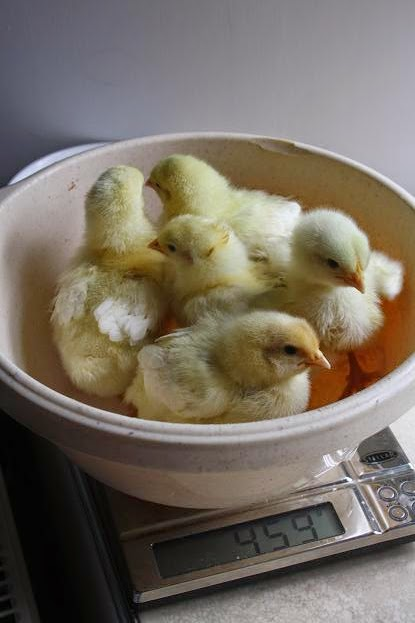
\includegraphics[width=\linewidth]{/Users/Nathaniel/Dropbox/Git/YaRrr_Book/media/chickweight.jpg}
\caption{I tried ordering a vegan alternative at a traditional German restaurant and this is what I got.}
\label{fig:chickweight}
\end{marginfigure}

\begin{footnotesize}
\begin{knitrout}
\definecolor{shadecolor}{rgb}{0.969, 0.969, 0.969}\color{fgcolor}\begin{kframe}
\begin{alltt}
\hlstd{ChickWeight[}\hlnum{1}\hlopt{:}\hlnum{5}\hlstd{,} \hlnum{1}\hlstd{]} \hlcom{# Give me rows 1 through 5 in column 1}
\end{alltt}
\begin{verbatim}
## [1] 42 51 59 64 76
\end{verbatim}
\begin{alltt}
\hlstd{ChickWeight[}\hlnum{2}\hlopt{:}\hlnum{6}\hlstd{,} \hlnum{2}\hlopt{:}\hlnum{3}\hlstd{]} \hlcom{# Give me rows 2 through 6 in columns 2 and 3}
\end{alltt}
\begin{verbatim}
##   Time Chick
## 2    2     1
## 3    4     1
## 4    6     1
## 5    8     1
## 6   10     1
\end{verbatim}
\begin{alltt}
\hlstd{ChickWeight[}\hlkwd{seq}\hlstd{(}\hlkwc{from} \hlstd{=} \hlnum{1}\hlstd{,} \hlkwc{to} \hlstd{=} \hlkwd{nrow}\hlstd{(ChickWeight),} \hlkwc{by} \hlstd{=} \hlnum{10}\hlstd{),} \hlnum{3}\hlstd{]} \hlcom{# Give me every 10th row in the 3rd column}
\end{alltt}
\begin{verbatim}
##  [1] 1  1  2  3  4  5  6  6  7  8  9  10 11 11 12 13 14 15 16 17 19 20 21
## [24] 21 22 23 24 25 26 26 27 28 29 30 31 31 32 33 34 35 36 36 37 38 39 40
## [47] 41 41 42 43 44 45 46 47 47 48 49 50
## 50 Levels: 18 < 16 < 15 < 13 < 9 < 20 < 10 < 8 < 17 < 19 < 4 < ... < 48
\end{verbatim}
\end{kframe}
\end{knitrout}
\end{footnotesize}
\marginnote{Here you can see the benefits of using \texttt{nrow()} - I used it to make sure I gave valid index values to \texttt{ChickWeight}}

If you want an entire row or column, you can simply leave one of the indices blank. For example, if I want the entire first row of \texttt{ChickWeight} and all of the columns, I can simply leave the column index blank:

\begin{footnotesize}
\begin{knitrout}
\definecolor{shadecolor}{rgb}{0.969, 0.969, 0.969}\color{fgcolor}\begin{kframe}
\begin{alltt}
\hlstd{ChickWeight[}\hlnum{1}\hlstd{,]}
\end{alltt}
\begin{verbatim}
##   weight Time Chick Diet
## 1     42    0     1    1
\end{verbatim}
\end{kframe}
\end{knitrout}
\end{footnotesize}

You can use the same logic to get an entire column of a dataframe by leaving the index for rows blank. If you leave both index values blank, you'll get the entire dataframe back.

\subsection{Accessing dataframe columns by column name and \$}

One of the nice things about dataframes is that each column will have a name. You can then use this name to access specific columns without having to index columns by numbers. To access the names of a dataframe, use the function \texttt{names()}. This will return a string vector with the names of the dataframe.

Let's use \texttt{names()} to get the names of some of the dataframes stored in R.

\begin{footnotesize}
\begin{knitrout}
\definecolor{shadecolor}{rgb}{0.969, 0.969, 0.969}\color{fgcolor}\begin{kframe}
\begin{alltt}
\hlkwd{names}\hlstd{(ChickWeight)}
\end{alltt}
\begin{verbatim}
## [1] "weight" "Time"   "Chick"  "Diet"
\end{verbatim}
\begin{alltt}
\hlkwd{names}\hlstd{(InsectSprays)}
\end{alltt}
\begin{verbatim}
## [1] "count" "spray"
\end{verbatim}
\begin{alltt}
\hlkwd{names}\hlstd{(ToothGrowth)}
\end{alltt}
\begin{verbatim}
## [1] "len"  "supp" "dose"
\end{verbatim}
\end{kframe}
\end{knitrout}
\end{footnotesize}

To access a specific column in a dataframe by name, you use the the \texttt{\$} operator:

\newfun{dataframe\$colname}

where \texttt{dataframe} is the name of the dataframe, and \texttt{colname} is the name of the column you are interested in. When you apply the \texttt{\$} operator to a dataframe, it will return a vector. Let's access some of the vectors in the dataframes \texttt{ChickWeight}, and \texttt{ToothGrowth}

\begin{footnotesize}
\begin{knitrout}
\definecolor{shadecolor}{rgb}{0.969, 0.969, 0.969}\color{fgcolor}\begin{kframe}
\begin{alltt}
\hlstd{ChickWeight}\hlopt{$}\hlstd{weight[}\hlnum{1}\hlopt{:}\hlnum{20}\hlstd{]} \hlcom{# Just the first 20 values}
\end{alltt}
\begin{verbatim}
##  [1]  42  51  59  64  76  93 106 125 149 171 199 205  40  49  58  72  84
## [18] 103 122 138
\end{verbatim}
\begin{alltt}
\hlstd{ToothGrowth}\hlopt{$}\hlstd{len}
\end{alltt}
\begin{verbatim}
##  [1]  4.2 11.5  7.3  5.8  6.4 10.0 11.2 11.2  5.2  7.0 16.5 16.5 15.2 17.3
## [15] 22.5 17.3 13.6 14.5 18.8 15.5 23.6 18.5 33.9 25.5 26.4 32.5 26.7 21.5
## [29] 23.3 29.5 15.2 21.5 17.6  9.7 14.5 10.0  8.2  9.4 16.5  9.7 19.7 23.3
## [43] 23.6 26.4 20.0 25.2 25.8 21.2 14.5 27.3 25.5 26.4 22.4 24.5 24.8 30.9
## [57] 26.4 27.3 29.4 23.0
\end{verbatim}
\end{kframe}
\end{knitrout}
\end{footnotesize}

Because the \$ operator returns a vector, you can easily calculate descriptive statistics on columns of a dataframe using \$:

\begin{footnotesize}
\begin{knitrout}
\definecolor{shadecolor}{rgb}{0.969, 0.969, 0.969}\color{fgcolor}\begin{kframe}
\begin{alltt}
\hlkwd{mean}\hlstd{(ChickWeight}\hlopt{$}\hlstd{weight)}
\end{alltt}
\begin{verbatim}
## [1] 121.8183
\end{verbatim}
\begin{alltt}
\hlkwd{median}\hlstd{(ToothGrowth}\hlopt{$}\hlstd{len)}
\end{alltt}
\begin{verbatim}
## [1] 19.25
\end{verbatim}
\end{kframe}
\end{knitrout}
\end{footnotesize}

\section{Adding new columns to a dataframe}

You can easily add columns to a dataframe using the \texttt{\$} and assignment \texttt{<-} operators. To do this, just use the \texttt{dataframe\$colname} notation and assign a new vector to it. Let's test this by adding a new column to \texttt{ChickWeight} called \texttt{height} which indicates the height of each chick at each time point. Now, because I don't have the actual height data, I'll just sample some random data from a normal distribution with mean 5 and standard deviation 1.

\begin{footnotesize}
\begin{knitrout}
\definecolor{shadecolor}{rgb}{0.969, 0.969, 0.969}\color{fgcolor}\begin{kframe}
\begin{alltt}
\hlstd{ChickWeight}\hlopt{$}\hlstd{height} \hlkwb{<-} \hlkwd{rnorm}\hlstd{(}\hlkwc{n} \hlstd{=} \hlkwd{nrow}\hlstd{(ChickWeight),} \hlkwc{mean} \hlstd{=} \hlnum{5}\hlstd{,} \hlkwc{sd} \hlstd{=} \hlnum{1}\hlstd{)}
\end{alltt}
\end{kframe}
\end{knitrout}
\end{footnotesize}

Let's look at the first few rows of \texttt{ChickWeight} to make sure it worked:

\begin{footnotesize}
\begin{knitrout}
\definecolor{shadecolor}{rgb}{0.969, 0.969, 0.969}\color{fgcolor}\begin{kframe}
\begin{alltt}
\hlkwd{head}\hlstd{(ChickWeight)}
\end{alltt}
\begin{verbatim}
##   weight Time Chick Diet   height
## 1     42    0     1    1 5.617418
## 2     51    2     1    1 4.719336
## 3     59    4     1    1 5.475568
## 4     64    6     1    1 4.449876
## 5     76    8     1    1 4.742738
## 6     93   10     1    1 5.641287
\end{verbatim}
\end{kframe}
\end{knitrout}
\end{footnotesize}

As you can see, the \texttt{ChickWeight} dataframe now has a column named \texttt{height} with the random data we generated.

Of course, because columns of dataframes are just vectors, you can add columns that are some function of existing columns. For example, let's add a column to \texttt{ChickWeight} called \texttt{density} which we'll define as each chick's height divided by its weight:

\begin{footnotesize}
\begin{knitrout}
\definecolor{shadecolor}{rgb}{0.969, 0.969, 0.969}\color{fgcolor}\begin{kframe}
\begin{alltt}
\hlstd{ChickWeight}\hlopt{$}\hlstd{density} \hlkwb{<-} \hlstd{ChickWeight}\hlopt{$}\hlstd{height} \hlopt{/} \hlstd{ChickWeight}\hlopt{$}\hlstd{weight}
\hlkwd{head}\hlstd{(ChickWeight)}
\end{alltt}
\begin{verbatim}
##   weight Time Chick Diet   height    density
## 1     42    0     1    1 5.617418 0.13374805
## 2     51    2     1    1 4.719336 0.09253599
## 3     59    4     1    1 5.475568 0.09280624
## 4     64    6     1    1 4.449876 0.06952931
## 5     76    8     1    1 4.742738 0.06240445
## 6     93   10     1    1 5.641287 0.06065900
\end{verbatim}
\end{kframe}
\end{knitrout}
\end{footnotesize}

When you are conducting analyses on dataframes, it's important that you always repeat the name of the dataframe when accessing its columns. If you don't, R will assume the column name is a totally different object. For example, the following code \textit{won't work} because R thinks that \texttt{height} and \texttt{weight} are totally separate objects from \texttt{ChickWeight}}

\begin{footnotesize}
\begin{knitrout}
\definecolor{shadecolor}{rgb}{0.969, 0.969, 0.969}\color{fgcolor}\begin{kframe}
\begin{alltt}
\hlstd{ChickWeight}\hlopt{$}\hlstd{density} \hlkwb{<-} \hlstd{height} \hlopt{/} \hlstd{weight} \hlcom{# BAD CODE!}
\end{alltt}
\end{kframe}
\end{knitrout}
\end{footnotesize}

However, there is a function \texttt{with()} that can help prevent you from having to repeat the name of a dataframe over and over again.

\newfun{with(x, ...)}\index{with()}

\marginnote{\texttt{with(x, ...)}: Simplifies your code for dataframe manipulation by allowing you to just enter the name of the dataframe once.}

The function \texttt{with()} allows you to specify a dataframe (or any other object in R) once, and R will assume you're referring to that object in an expression.

For example, let's repeat the \texttt{ChickWeight\$density} calculation using \texttt{with()}. We'll set the name of the dataframe as the first argument, then do our regular calculations on the column names.

\begin{footnotesize}
\begin{knitrout}
\definecolor{shadecolor}{rgb}{0.969, 0.969, 0.969}\color{fgcolor}\begin{kframe}
\begin{alltt}
\hlstd{ChickWeight}\hlopt{$}\hlstd{density} \hlkwb{<-} \hlkwd{with}\hlstd{(ChickWeight, height} \hlopt{/} \hlstd{weight)}
\end{alltt}
\end{kframe}
\end{knitrout}
\end{footnotesize}

As you can imagine, if you're performing a long set of calculations on many columns of a dataframe, the \texttt{with()} function can save you lots of typing!


\section{Centering and standardizing (z-score) data}

Centering and standardizing are two common methods of transforming data. Centering data simply means transforming the data so that the mean is 0, while standardizing data means centering the data and dividing all data points by the standard deviation of the data. Here's how to do each:

\subsubsection{Centering}

Centering data is quite easy. All you need to do is calculate the mean of a vector, then subtract that mean from all data in the vector.

Generally, if we have a dataframe called \texttt{df}, and we want to center a column called \texttt{x}, we'd run the following code:

\begin{knitrout}
\definecolor{shadecolor}{rgb}{0.969, 0.969, 0.969}\color{fgcolor}\begin{kframe}
\begin{alltt}
\hlstd{df}\hlopt{$}\hlstd{x.centered} \hlkwb{<-} \hlkwd{with}\hlstd{(df, x} \hlopt{-} \hlkwd{mean}\hlstd{(x))}
\end{alltt}
\end{kframe}
\end{knitrout}

Let's use this method to center the weight data from \texttt{ChickWeight} - we'll call the new column \texttt{weight.c}

\begin{footnotesize}
\begin{knitrout}
\definecolor{shadecolor}{rgb}{0.969, 0.969, 0.969}\color{fgcolor}\begin{kframe}
\begin{alltt}
\hlstd{ChickWeight}\hlopt{$}\hlstd{weight.c} \hlkwb{<-} \hlkwd{with}\hlstd{(ChickWeight, weight} \hlopt{-} \hlkwd{mean}\hlstd{(weight))}
\end{alltt}
\end{kframe}
\end{knitrout}
\end{footnotesize}

To see if this worked, let's compare the mean of \texttt{weight} and \texttt{weight.c}

\begin{footnotesize}
\begin{knitrout}
\definecolor{shadecolor}{rgb}{0.969, 0.969, 0.969}\color{fgcolor}\begin{kframe}
\begin{alltt}
\hlkwd{mean}\hlstd{(ChickWeight}\hlopt{$}\hlstd{weight)}
\end{alltt}
\begin{verbatim}
## [1] 121.8183
\end{verbatim}
\begin{alltt}
\hlkwd{mean}\hlstd{(ChickWeight}\hlopt{$}\hlstd{weight.c)}
\end{alltt}
\begin{verbatim}
## [1] -1.219277e-15
\end{verbatim}
\end{kframe}
\end{knitrout}
\end{footnotesize}

I know what you're thinking...``But wait!!! The mean of \texttt{ChickWeight\$weight.c} isn't exactly 0!!!'' Don't worry, \texttt{-1.2919e-15} is -0000000000000012919. For all intents and purposes, that's equal to 0 - the reason it's not \textit{exactly} 0 is due to peculiarities about how computers represent numbers. Don't ask me why, I'm just a pirate.

\subsubsection{Standardizing}

Standardizing data is almost as easy as centering. The only difference is that, in addition to subtracting the mean from the data, we need to divide the data by its standard deviation. If you have a dataframe \texttt{df} and you want to standardize a column \texttt{x} into a new column called \texttt{x.z}, we use the following code:

\begin{knitrout}
\definecolor{shadecolor}{rgb}{0.969, 0.969, 0.969}\color{fgcolor}\begin{kframe}
\begin{alltt}
\hlcom{# Create a standardized version of column x in a dataframe df}
\hlstd{df}\hlopt{$}\hlstd{x.z} \hlkwb{<-} \hlkwd{with}\hlstd{(df, (x} \hlopt{-} \hlkwd{mean}\hlstd{(x))} \hlopt{/} \hlkwd{sd}\hlstd{(x))}
\end{alltt}
\end{kframe}
\end{knitrout}

Let's use this method to standardize the weight data from \texttt{ChickWeight} - we'll call the new column \texttt{weight.z}

\begin{footnotesize}
\begin{knitrout}
\definecolor{shadecolor}{rgb}{0.969, 0.969, 0.969}\color{fgcolor}\begin{kframe}
\begin{alltt}
\hlstd{ChickWeight}\hlopt{$}\hlstd{weight.z} \hlkwb{<-} \hlkwd{with}\hlstd{(ChickWeight, (weight} \hlopt{-} \hlkwd{mean}\hlstd{(weight))} \hlopt{/} \hlkwd{sd}\hlstd{(weight))}
\end{alltt}
\end{kframe}
\end{knitrout}
\end{footnotesize}

To see if this worked, let's compare the mean of \texttt{weight}, \texttt{weight.c}, and \texttt{weight.z}. The mean of \texttt{weight.z} should be 0 and its standard deviation should be 1:

\begin{footnotesize}
\begin{knitrout}
\definecolor{shadecolor}{rgb}{0.969, 0.969, 0.969}\color{fgcolor}\begin{kframe}
\begin{alltt}
\hlkwd{c}\hlstd{(}\hlkwd{mean}\hlstd{(ChickWeight}\hlopt{$}\hlstd{weight),} \hlkwd{sd}\hlstd{(ChickWeight}\hlopt{$}\hlstd{weight))}
\end{alltt}
\begin{verbatim}
## [1] 121.81834  71.07196
\end{verbatim}
\begin{alltt}
\hlkwd{c}\hlstd{(}\hlkwd{mean}\hlstd{(ChickWeight}\hlopt{$}\hlstd{weight.c),} \hlkwd{sd}\hlstd{(ChickWeight}\hlopt{$}\hlstd{weight.c))}
\end{alltt}
\begin{verbatim}
## [1] -1.219277e-15  7.107196e+01
\end{verbatim}
\begin{alltt}
\hlkwd{c}\hlstd{(}\hlkwd{mean}\hlstd{(ChickWeight}\hlopt{$}\hlstd{weight.z),} \hlkwd{sd}\hlstd{(ChickWeight}\hlopt{$}\hlstd{weight.z))}
\end{alltt}
\begin{verbatim}
## [1] -1.194348e-17  1.000000e+00
\end{verbatim}
\end{kframe}
\end{knitrout}
\end{footnotesize}


\section{Subsetting dataframes with logical indexing and subset()}

Frequently you will want to access specific rows of a dataframe based on some criteria - this is called subsetting. For example, we may want to look just at the data from females in our survey data. To do this, we can use one of two methods: indexing with logical vectors, or the \texttt{subset()} function.

Indexing dataframes with logical vectors is very similar to indexing data vectors. First, we create a logical vector. Next, we index the dataframe using that logical vector. Let's use indexing to access just the data from Chick 1 in \texttt{ChickWeight}:

\begin{footnotesize}
\begin{knitrout}
\definecolor{shadecolor}{rgb}{0.969, 0.969, 0.969}\color{fgcolor}\begin{kframe}
\begin{alltt}
\hlstd{chick1.log} \hlkwb{<-} \hlstd{ChickWeight}\hlopt{$}\hlstd{Chick} \hlopt{==} \hlnum{1} \hlcom{# Step 1: Create a logical vector}
\hlstd{chick1.data} \hlkwb{<-} \hlstd{ChickWeight[chick1.log,]} \hlcom{# Step 2: Index dataframe by logical vector}
\hlstd{chick1.data} \hlcom{# Print the result}
\end{alltt}
\begin{verbatim}
##    weight Time Chick Diet   height    density   weight.c    weight.z
## 1      42    0     1    1 5.617418 0.13374805 -79.818339 -1.12306372
## 2      51    2     1    1 4.719336 0.09253599 -70.818339 -0.99643150
## 3      59    4     1    1 5.475568 0.09280624 -62.818339 -0.88386952
## 4      64    6     1    1 4.449876 0.06952931 -57.818339 -0.81351829
## 5      76    8     1    1 4.742738 0.06240445 -45.818339 -0.64467533
## 6      93   10     1    1 5.641287 0.06065900 -28.818339 -0.40548114
## 7     106   12     1    1 3.082565 0.02908081 -15.818339 -0.22256793
## 8     125   14     1    1 3.784443 0.03027554   3.181661  0.04476675
## 9     149   16     1    1 6.087122 0.04085317  27.181661  0.38245267
## 10    171   18     1    1 5.127636 0.02998618  49.181661  0.69199810
## 11    199   20     1    1 6.022833 0.03026549  77.181661  1.08596500
## 12    205   21     1    1 4.743539 0.02313921  83.181661  1.17038648
\end{verbatim}
\end{kframe}
\end{knitrout}
\end{footnotesize}

If you'd like, you can also combine the two steps in one line. For example, the following code gives the same result as the previous:

\begin{footnotesize}
\begin{knitrout}
\definecolor{shadecolor}{rgb}{0.969, 0.969, 0.969}\color{fgcolor}\begin{kframe}
\begin{alltt}
\hlstd{chick1.data} \hlkwb{<-} \hlstd{ChickWeight[ChickWeight}\hlopt{$}\hlstd{Chick} \hlopt{==} \hlnum{1}\hlstd{, ]} \hlcom{# Two steps in 1}
\end{alltt}
\end{kframe}
\end{knitrout}
\end{footnotesize}

Now, let's try indexing the \texttt{ChickWeight} data using a slightly more complicated index. For example, let's access just the data for the chicks where \texttt{Time} is less than 10

\begin{footnotesize}
\begin{knitrout}
\definecolor{shadecolor}{rgb}{0.969, 0.969, 0.969}\color{fgcolor}\begin{kframe}
\begin{alltt}
\hlstd{ChickWeight.lt10} \hlkwb{<-} \hlstd{ChickWeight[ChickWeight}\hlopt{$}\hlstd{Time} \hlopt{<} \hlnum{10}\hlstd{,]}
\hlkwd{head}\hlstd{(ChickWeight.lt10)}
\end{alltt}
\begin{verbatim}
##    weight Time Chick Diet   height    density  weight.c   weight.z
## 1      42    0     1    1 5.617418 0.13374805 -79.81834 -1.1230637
## 2      51    2     1    1 4.719336 0.09253599 -70.81834 -0.9964315
## 3      59    4     1    1 5.475568 0.09280624 -62.81834 -0.8838695
## 4      64    6     1    1 4.449876 0.06952931 -57.81834 -0.8135183
## 5      76    8     1    1 4.742738 0.06240445 -45.81834 -0.6446753
## 13     40    0     2    1 5.495245 0.13738111 -81.81834 -1.1512042
\end{verbatim}
\end{kframe}
\end{knitrout}
\end{footnotesize}

Indexing with brackets is the standard way to slice and dice dataframes. However, if you are working on data that is all in the same dataframe, it can get a bit tiresome to have to constantly repeat the name of the dataframe. For example, let's say we wanted to get data from \texttt{ChickWeight} where \texttt{Time < 10} and \texttt{Diet == 1}. The following code works, but it's a bit tedious:

\begin{footnotesize}
\begin{knitrout}
\definecolor{shadecolor}{rgb}{0.969, 0.969, 0.969}\color{fgcolor}\begin{kframe}
\begin{alltt}
\hlstd{mydata} \hlkwb{<-} \hlstd{ChickWeight[ChickWeight}\hlopt{$}\hlstd{Time} \hlopt{<} \hlnum{10} \hlopt{&} \hlstd{ChickWeight}\hlopt{$}\hlstd{Diet} \hlopt{==} \hlnum{1}\hlstd{,]}
\end{alltt}
\end{kframe}
\end{knitrout}
\end{footnotesize}

A way to get around having to repeat the name of the dataframe over and over is to use the \texttt{subset()} function.



\vspace{5mm} %5mm vertical space
\noindent
\setlength{\fboxrule}{1.5pt}
\fbox{
\parbox{\textwidth}{

\newfun{subset()}\index{subset()}

\hline

\begin{description}

  \item[\tt{x}] \hfill \\
      The data (usually a dataframe)
        \item[\tt{subset}] \hfill \\
      A logical vector indicating which rows you want to select
        \item[\tt{select}] \hfill \\
      An optional vector of the columns you want to select
       
\end{description}

}
}
\vspace{5mm} %5mm vertical space

For example, let's get the \texttt{ChickWeight} data for \texttt{Diet == 1} and \texttt{Time > 15}

\begin{footnotesize}
\begin{knitrout}
\definecolor{shadecolor}{rgb}{0.969, 0.969, 0.969}\color{fgcolor}\begin{kframe}
\begin{alltt}
\hlstd{data} \hlkwb{<-} \hlkwd{subset}\hlstd{(}\hlkwc{x} \hlstd{= ChickWeight,}
               \hlkwc{subset} \hlstd{= (Diet} \hlopt{==} \hlnum{1} \hlopt{&} \hlstd{Time} \hlopt{>} \hlnum{15}\hlstd{)}
               \hlstd{)}
\hlkwd{head}\hlstd{(data)}
\end{alltt}
\begin{verbatim}
##    weight Time Chick Diet   height    density weight.c  weight.z
## 9     149   16     1    1 6.087122 0.04085317 27.18166 0.3824527
## 10    171   18     1    1 5.127636 0.02998618 49.18166 0.6919981
## 11    199   20     1    1 6.022833 0.03026549 77.18166 1.0859650
## 12    205   21     1    1 4.743539 0.02313921 83.18166 1.1703865
## 21    162   16     2    1 4.671985 0.02883942 40.18166 0.5653659
## 22    187   18     2    1 4.280018 0.02288780 65.18166 0.9171220
\end{verbatim}
\end{kframe}
\end{knitrout}
\end{footnotesize}

In the example above, I didn't specify an input to the \texttt{select} argument because I wanted all columns. However, if you just want certain columns, you can just name the columns you want. For example, let's say I just want the \texttt{weight} and \texttt{Time}
 columns from the previous analysis. To do this, I'll just add the column names as inputs to the \textt{select} argument:
 
 \begin{footnotesize}
\begin{knitrout}
\definecolor{shadecolor}{rgb}{0.969, 0.969, 0.969}\color{fgcolor}\begin{kframe}
\begin{alltt}
\hlstd{data} \hlkwb{<-} \hlkwd{subset}\hlstd{(}\hlkwc{x} \hlstd{= ChickWeight,}
               \hlkwc{subset} \hlstd{= (Diet} \hlopt{==} \hlnum{1} \hlopt{&} \hlstd{Time} \hlopt{>} \hlnum{15}\hlstd{),}
               \hlkwc{select} \hlstd{=} \hlkwd{c}\hlstd{(weight, Time)}
               \hlstd{)}
\hlkwd{head}\hlstd{(data)}
\end{alltt}
\begin{verbatim}
##    weight Time
## 9     149   16
## 10    171   18
## 11    199   20
## 12    205   21
## 21    162   16
## 22    187   18
\end{verbatim}
\end{kframe}
\end{knitrout}
\end{footnotesize}
 
\section{Combining indexing and descriptive statistics}

Once you know how to index a dataframe to get the data vectors you want, you can then easily calculate descriptive statistics based on specific criteria. For example, let's calculate the mean weight of the chicks on \texttt{Diet == 1}. To show you that there are many ways to do this, I'll write the code in three different ways:

\begin{footnotesize}
\begin{knitrout}
\definecolor{shadecolor}{rgb}{0.969, 0.969, 0.969}\color{fgcolor}\begin{kframe}
\begin{alltt}
\hlcom{# What is the mean weight of chicks on the first diet?}

\hlkwd{mean}\hlstd{(ChickWeight}\hlopt{$}\hlstd{weight[ChickWeight}\hlopt{$}\hlstd{Diet} \hlopt{==} \hlnum{1}\hlstd{])} \hlcom{# Using logical indexing}
\end{alltt}
\begin{verbatim}
## [1] 102.6455
\end{verbatim}
\begin{alltt}
\hlkwd{with}\hlstd{(ChickWeight,} \hlkwd{mean}\hlstd{(weight[Diet} \hlopt{==} \hlnum{1}\hlstd{]))} \hlcom{# Logical indexing and with()}
\end{alltt}
\begin{verbatim}
## [1] 102.6455
\end{verbatim}
\begin{alltt}
\hlkwd{mean}\hlstd{(}\hlkwd{subset}\hlstd{(}\hlkwc{x} \hlstd{= ChickWeight,} \hlkwc{subset} \hlstd{= Diet} \hlopt{==} \hlnum{1}\hlstd{)}\hlopt{$}\hlstd{weight)} \hlcom{# Using subset()}
\end{alltt}
\begin{verbatim}
## [1] 102.6455
\end{verbatim}
\end{kframe}
\end{knitrout}
\end{footnotesize}

As you can see, there are many ways to do the same thing in R. Ultimately, the choice of which specific code and functions you use is up to you.

\section{A worked example: Credit default}

For this example, we'll work with a dataset called \texttt{credit}. This dataset contains information about German loan borrowers (IVs) and whether or not the borrower defaulted on their loan (DV). To load the dataset, either download and load the data from the link \texttt{http://goo.gl/a7umut}, or simply run the following code:

\begin{footnotesize}
\begin{knitrout}
\definecolor{shadecolor}{rgb}{0.969, 0.969, 0.969}\color{fgcolor}\begin{kframe}
\begin{alltt}
\hlstd{credit} \hlkwb{<-} \hlkwd{read.table}\hlstd{(}\hlstr{"http://nathanieldphillips.com/wp-content/uploads/2015/05/credit.csv"}\hlstd{,}
                     \hlkwc{sep} \hlstd{=} \hlstr{","}\hlstd{,} \hlkwc{header} \hlstd{= T,} \hlkwc{stringsAsFactors} \hlstd{= F)}
\end{alltt}
\end{kframe}
\end{knitrout}
\end{footnotesize}

Here is a screenshot of the dataset:

\begin{footnotesize}
\begin{knitrout}
\definecolor{shadecolor}{rgb}{0.969, 0.969, 0.969}\color{fgcolor}\begin{kframe}
\begin{alltt}
\hlkwd{View}\hlstd{(credit)}
\end{alltt}
\end{kframe}
\end{knitrout}
\end{footnotesize}

\begin{figure}
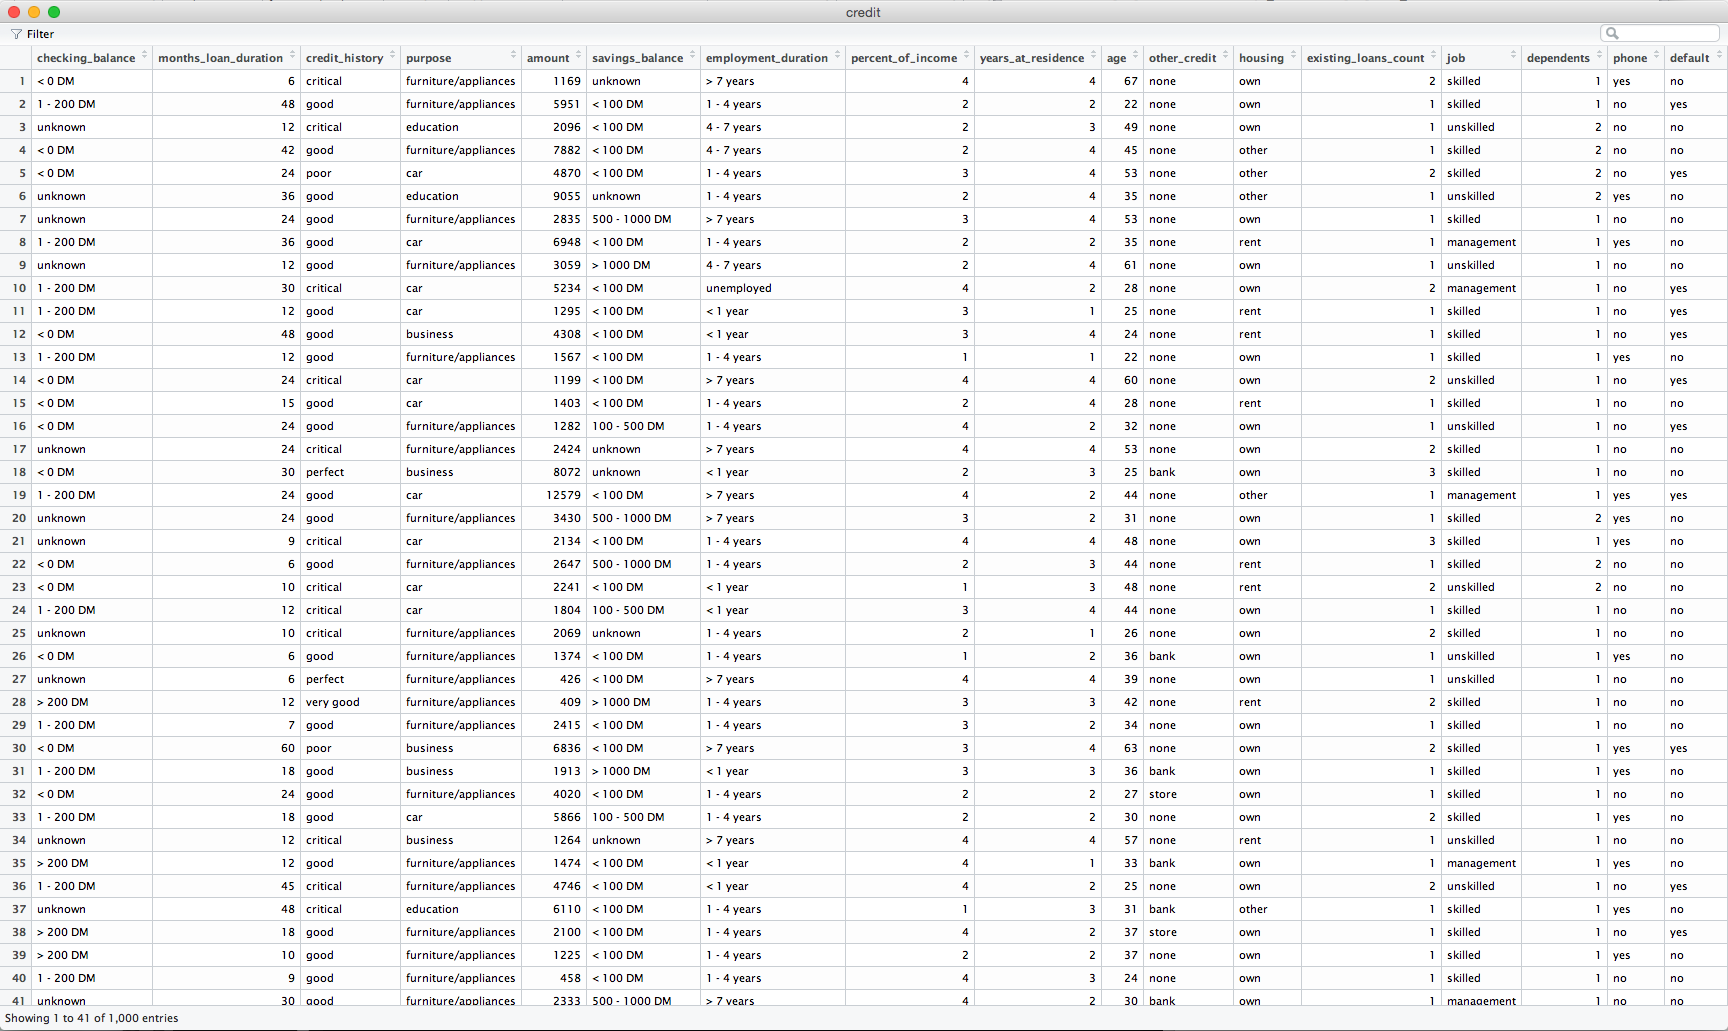
\includegraphics[width=\linewidth]{/Users/Nathaniel/Dropbox/Git/YaRrr_Book/media/creditscreenshot.png}
\caption{Screenshot of the credit dataset.}
\label{fig:creditscreen}
\end{figure}

The dataset has 17 total columns - to see their names, execute \texttt{names(credit)}

\begin{footnotesize}
\begin{knitrout}
\definecolor{shadecolor}{rgb}{0.969, 0.969, 0.969}\color{fgcolor}\begin{kframe}
\begin{alltt}
\hlkwd{names}\hlstd{(credit)}
\end{alltt}
\begin{verbatim}
##  [1] "checking_balance"     "months_loan_duration" "credit_history"      
##  [4] "purpose"              "amount"               "savings_balance"     
##  [7] "employment_duration"  "percent_of_income"    "years_at_residence"  
## [10] "age"                  "other_credit"         "housing"             
## [13] "existing_loans_count" "job"                  "dependents"          
## [16] "phone"                "default"
\end{verbatim}
\end{kframe}
\end{knitrout}
\end{footnotesize}

Let's answer 5 questions with this dataset:

\begin{enumerate}

  \item Was there a relationship between the size of the loan and whether or not it defaulted?
  
    
\begin{marginfigure}
\begin{tiny}
\begin{knitrout}
\definecolor{shadecolor}{rgb}{0.969, 0.969, 0.969}\color{fgcolor}\begin{kframe}
\begin{alltt}
\hlstd{amount.default} \hlkwb{<-} \hlstd{credit}\hlopt{$}\hlstd{amount[credit}\hlopt{$}\hlstd{default} \hlopt{==} \hlstr{"yes"}\hlstd{]}
\hlstd{amount.nodefault} \hlkwb{<-} \hlstd{credit}\hlopt{$}\hlstd{amount[credit}\hlopt{$}\hlstd{default} \hlopt{==} \hlstr{"no"}\hlstd{]}

\hlkwd{require}\hlstd{(beanplot)}
\end{alltt}


{\ttfamily\noindent\itshape\color{messagecolor}{\#\# Loading required package: beanplot}}\begin{alltt}
\hlkwd{beanplot}\hlstd{(amount} \hlopt{~} \hlstd{default,} \hlkwc{data} \hlstd{= credit,}
         \hlkwc{col} \hlstd{=} \hlkwd{c}\hlstd{(}\hlstr{"white"}\hlstd{,} \hlkwd{gray}\hlstd{(}\hlnum{.8}\hlstd{),} \hlkwd{gray}\hlstd{(}\hlnum{.8}\hlstd{),} \hlstr{"black"}\hlstd{),}
         \hlkwc{names} \hlstd{=} \hlkwd{c}\hlstd{(}\hlstr{"No"}\hlstd{,} \hlstr{"Yes"}\hlstd{),}
         \hlkwc{main} \hlstd{=} \hlstr{"Loan size by default"}\hlstd{,}
         \hlkwc{xlab} \hlstd{=} \hlstr{"Did the loan default?"}\hlstd{,}
         \hlkwc{ylab} \hlstd{=} \hlstr{"Loan size (log-transformed)"}\hlstd{,}
         \hlkwc{what} \hlstd{=} \hlkwd{c}\hlstd{(}\hlnum{1}\hlstd{,} \hlnum{1}\hlstd{,} \hlnum{1}\hlstd{,} \hlnum{0}\hlstd{)}
         \hlstd{)}
\end{alltt}


{\ttfamily\noindent\itshape\color{messagecolor}{\#\# log="{}y"{} selected}}\end{kframe}
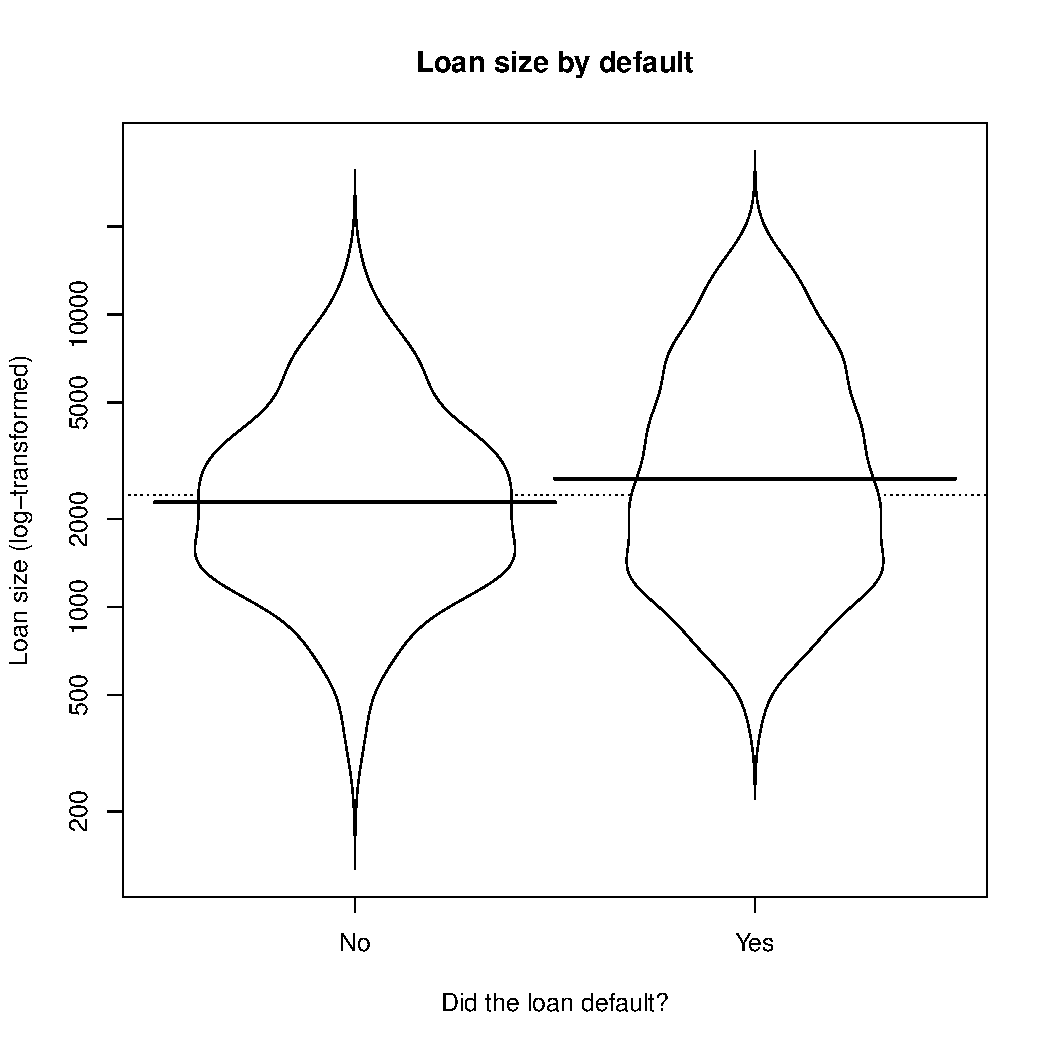
\includegraphics[width=\maxwidth]{figure/unnamed-chunk-132-1} 

\end{knitrout}
\end{tiny}
\caption{Distributions of loan sizes separated for loans that defaulted and those that did not.}
\label{fig:creditbeans}
\end{marginfigure}
  
\begin{footnotesize}
\begin{knitrout}
\definecolor{shadecolor}{rgb}{0.969, 0.969, 0.969}\color{fgcolor}\begin{kframe}
\begin{alltt}
\hlstd{amount.default} \hlkwb{<-} \hlstd{credit}\hlopt{$}\hlstd{amount[credit}\hlopt{$}\hlstd{default} \hlopt{==} \hlstr{"yes"}\hlstd{]}
\hlstd{amount.nodefault} \hlkwb{<-} \hlstd{credit}\hlopt{$}\hlstd{amount[credit}\hlopt{$}\hlstd{default} \hlopt{==} \hlstr{"no"}\hlstd{]}

\hlkwd{summary}\hlstd{(amount.default)}
\end{alltt}
\begin{verbatim}
##    Min. 1st Qu.  Median    Mean 3rd Qu.    Max. 
##     433    1352    2574    3938    5142   18420
\end{verbatim}
\begin{alltt}
\hlkwd{summary}\hlstd{(amount.nodefault)}
\end{alltt}
\begin{verbatim}
##    Min. 1st Qu.  Median    Mean 3rd Qu.    Max. 
##     250    1376    2244    2985    3635   15860
\end{verbatim}
\end{kframe}
\end{knitrout}
\end{footnotesize}

We calculated the median loan size separately for people whose loans defaulted and those whose loans did not default. The loan amounts of loans that defaulted (median of 2574) tended to be a bit larger than those that did not (median of 2244). However, looking at the full amount distributions (see Figure~\ref{fig:creditbeans}), it is unclear if the difference is really very meaningful.
  
  \item Was the age of the borrower related to the loan amount?
  
\begin{marginfigure}
\begin{tiny}
\begin{knitrout}
\definecolor{shadecolor}{rgb}{0.969, 0.969, 0.969}\color{fgcolor}\begin{kframe}
\begin{alltt}
\hlcom{# Main Plot}
\hlkwd{plot}\hlstd{(credit}\hlopt{$}\hlstd{age, credit}\hlopt{$}\hlstd{amount,}
     \hlkwc{pch} \hlstd{=} \hlnum{16}\hlstd{,} \hlkwc{col} \hlstd{=} \hlkwd{gray}\hlstd{(}\hlnum{.5}\hlstd{,} \hlkwc{alpha} \hlstd{=} \hlnum{.2}\hlstd{),}
     \hlkwc{main} \hlstd{=} \hlstr{"Loan amount by borrower age"}\hlstd{,}
     \hlkwc{xlab} \hlstd{=} \hlstr{"Borrower Age"}\hlstd{,} \hlkwc{ylab} \hlstd{=} \hlstr{"Loan Amount (DM)"}
     \hlstd{)}

\hlkwd{par}\hlstd{(}\hlkwc{xpd}\hlstd{=}\hlnum{NA}\hlstd{)}
\hlkwd{segments}\hlstd{(}\hlnum{25}\hlstd{,} \hlnum{20000}\hlstd{,} \hlnum{35}\hlstd{,} \hlnum{20000}\hlstd{,} \hlkwc{col} \hlstd{=} \hlstr{"red"}\hlstd{,} \hlkwc{lwd} \hlstd{=} \hlnum{2}\hlstd{)}
\hlkwd{text}\hlstd{(}\hlnum{50}\hlstd{,} \hlnum{20000}\hlstd{,} \hlstr{"5 year average"}\hlstd{)}

\hlcom{# Create factor from age}
\hlstd{age.cut} \hlkwb{<-} \hlkwd{cut}\hlstd{(credit}\hlopt{$}\hlstd{age,} \hlkwc{breaks} \hlstd{=} \hlkwd{seq}\hlstd{(}\hlnum{20}\hlstd{,} \hlnum{70}\hlstd{,} \hlnum{5}\hlstd{))}

\hlcom{# Determine mean loan by age factor}
\hlstd{amount.cut} \hlkwb{<-} \hlkwd{tapply}\hlstd{(credit}\hlopt{$}\hlstd{amount, age.cut, mean)}

\hlcom{# Add mean lines}
\hlkwd{lines}\hlstd{(}\hlkwd{seq}\hlstd{(}\hlnum{22.5}\hlstd{,} \hlnum{67.5}\hlstd{,} \hlnum{5}\hlstd{), amount.cut,}
      \hlkwc{col} \hlstd{=} \hlstr{"red"}\hlstd{,} \hlkwc{lwd} \hlstd{=} \hlnum{2}\hlstd{,} \hlkwc{type} \hlstd{=} \hlstr{"b"}\hlstd{,} \hlkwc{pch} \hlstd{=} \hlnum{16}\hlstd{)}
\end{alltt}
\end{kframe}
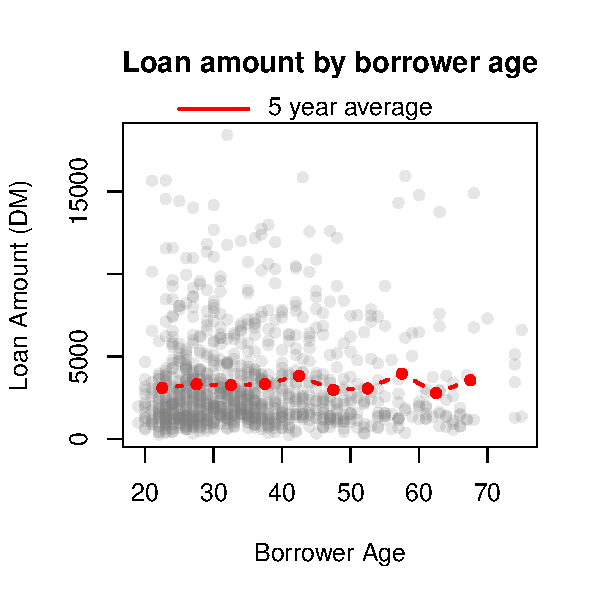
\includegraphics[width=\maxwidth]{figure/unnamed-chunk-134-1} 

\end{knitrout}
\end{tiny}
\caption{Distributions of loan sizes as a function of the age of the borrower.}
\label{fig:creditscatter}
\end{marginfigure}
  
\begin{footnotesize}
\begin{knitrout}
\definecolor{shadecolor}{rgb}{0.969, 0.969, 0.969}\color{fgcolor}\begin{kframe}
\begin{alltt}
\hlkwd{summary}\hlstd{(credit}\hlopt{$}\hlstd{amount[credit}\hlopt{$}\hlstd{age} \hlopt{<=} \hlkwd{median}\hlstd{(credit}\hlopt{$}\hlstd{age)])}
\end{alltt}
\begin{verbatim}
##    Min. 1st Qu.  Median    Mean 3rd Qu.    Max. 
##     276    1364    2310    3193    3924   18420
\end{verbatim}
\begin{alltt}
\hlkwd{summary}\hlstd{(credit}\hlopt{$}\hlstd{amount[credit}\hlopt{$}\hlstd{age} \hlopt{>} \hlkwd{median}\hlstd{(credit}\hlopt{$}\hlstd{age)])}
\end{alltt}
\begin{verbatim}
##    Min. 1st Qu.  Median    Mean 3rd Qu.    Max. 
##     250    1370    2324    3354    4042   15940
\end{verbatim}
\begin{alltt}
\hlkwd{cor}\hlstd{(credit}\hlopt{$}\hlstd{age, credit}\hlopt{$}\hlstd{amount)}
\end{alltt}
\begin{verbatim}
## [1] 0.03271642
\end{verbatim}
\end{kframe}
\end{knitrout}
\end{footnotesize}
  
  To answer this, we separately calculated the median loan amount for borrowers below and above the median age (of 33). Borrowers below the median age had a median loan amount of 2310, while borrowers above the median age had a median loan amount of 2324. This suggests that age was unrelated to loan amount. Examining the scatterplot in Figure~\ref{fig:creditscatter}, we do not find strong evidence for an effect of borrower age on loan amount. 
  
  \item Was there a relationship between whether or not someone had a phone and whether or not their loan defaulted?
  
\begin{footnotesize}
\begin{knitrout}
\definecolor{shadecolor}{rgb}{0.969, 0.969, 0.969}\color{fgcolor}\begin{kframe}
\begin{alltt}
\hlkwd{with}\hlstd{(credit,} \hlkwd{table}\hlstd{(phone, default))}
\end{alltt}
\begin{verbatim}
##      default
## phone  no yes
##   no  409 187
##   yes 291 113
\end{verbatim}
\begin{alltt}
\hlkwd{with}\hlstd{(credit[credit}\hlopt{$}\hlstd{phone} \hlopt{==} \hlstr{"yes"}\hlstd{,],} \hlkwd{mean}\hlstd{(default} \hlopt{==} \hlstr{"yes"}\hlstd{))}
\end{alltt}
\begin{verbatim}
## [1] 0.279703
\end{verbatim}
\begin{alltt}
\hlkwd{with}\hlstd{(credit[credit}\hlopt{$}\hlstd{phone} \hlopt{==} \hlstr{"no"}\hlstd{,],} \hlkwd{mean}\hlstd{(default} \hlopt{==} \hlstr{"yes"}\hlstd{))}
\end{alltt}
\begin{verbatim}
## [1] 0.3137584
\end{verbatim}
\end{kframe}
\end{knitrout}
\end{footnotesize}

We separately the proportion of people who defaulted on their loans separately between those who own a phone and those who do not. We found that people without a phone were slightly more likely to default (31.38\%) than people with a phone (27.97\%) (a \texttt{mosaic.plot} of the data is presented in margin Figure~\ref{fig:phoneloan}).
  
  
\end{enumerate}


\subsection{Additional Tips}

\begin{itemize}
  \item If you want to change the names of columns in a dataframe, you can do this by reassigning elements of the \texttt{names()} function. For example, let's change the names of the first two columns of our dataframe \texttt{survey} to "Sex" and "Height.cm"


\begin{marginfigure}
  \begin{tiny}
\begin{knitrout}
\definecolor{shadecolor}{rgb}{0.969, 0.969, 0.969}\color{fgcolor}\begin{kframe}
\begin{alltt}
\hlkwd{require}\hlstd{(RColorBrewer)}
\hlkwd{with}\hlstd{(credit,} \hlkwd{mosaicplot}\hlstd{(}\hlkwd{table}\hlstd{(phone, default),}
                  \hlkwc{main} \hlstd{=} \hlstr{"Phone Ownership and Loan Default"}\hlstd{,}
                  \hlkwc{xlab} \hlstd{=} \hlstr{"Own Phone?"}\hlstd{,}
                  \hlkwc{ylab} \hlstd{=} \hlstr{"Loan Default?"}\hlstd{,} \hlkwc{color} \hlstd{=} \hlkwd{brewer.pal}\hlstd{(}\hlnum{12}\hlstd{,} \hlstr{"Set3"}\hlstd{)[}\hlnum{5}\hlopt{:}\hlnum{4}\hlstd{]}
     \hlstd{))}

\hlstd{defper.withphone} \hlkwb{<-} \hlkwd{mean}\hlstd{(credit}\hlopt{$}\hlstd{default[credit}\hlopt{$}\hlstd{phone} \hlopt{==} \hlstr{"yes"}\hlstd{]} \hlopt{==} \hlstr{"yes"}\hlstd{)}
\hlstd{defper.nophone} \hlkwb{<-} \hlkwd{mean}\hlstd{(credit}\hlopt{$}\hlstd{default[credit}\hlopt{$}\hlstd{phone} \hlopt{==} \hlstr{"no"}\hlstd{]} \hlopt{==} \hlstr{"yes"}\hlstd{)}

\hlkwd{text}\hlstd{(}\hlkwd{mean}\hlstd{(credit}\hlopt{$}\hlstd{phone} \hlopt{==} \hlstr{"no"}\hlstd{)} \hlopt{/} \hlnum{2}\hlstd{,}
     \hlstd{defper.nophone} \hlopt{/} \hlnum{2}\hlstd{,}
     \hlkwd{paste}\hlstd{(}\hlnum{100} \hlopt{*} \hlkwd{round}\hlstd{(defper.nophone,} \hlnum{2}\hlstd{),} \hlstr{"%"}\hlstd{,} \hlkwc{sep} \hlstd{=} \hlstr{""}\hlstd{)}
     \hlstd{)}

\hlkwd{text}\hlstd{(}\hlnum{1} \hlopt{-} \hlkwd{mean}\hlstd{(credit}\hlopt{$}\hlstd{phone} \hlopt{==} \hlstr{"yes"}\hlstd{)} \hlopt{/} \hlnum{2}\hlstd{,}
     \hlstd{defper.withphone} \hlopt{/} \hlnum{2}\hlstd{,}
     \hlkwd{paste}\hlstd{(}\hlnum{100} \hlopt{*} \hlkwd{round}\hlstd{(defper.withphone,} \hlnum{2}\hlstd{),} \hlstr{"%"}\hlstd{,} \hlkwc{sep} \hlstd{=} \hlstr{""}\hlstd{)}
     \hlstd{)}
\end{alltt}
\end{kframe}
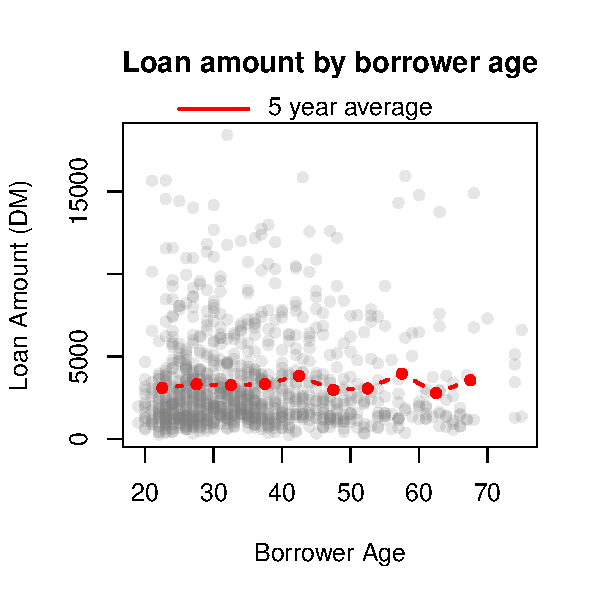
\includegraphics[width=\maxwidth]{figure/unnamed-chunk-137-1} 

\end{knitrout}
  \end{tiny}
  \label{fig:phoneloan}
  \caption{Mosaic plot of the contingency between phone ownership and loan defaults in the \texttt{credit} dataset. People who own a phone are slightly less likely to default on their loans that people who do not own a phone.}
  \end{marginfigure}


\begin{footnotesize}
\begin{knitrout}
\definecolor{shadecolor}{rgb}{0.969, 0.969, 0.969}\color{fgcolor}\begin{kframe}
\begin{alltt}
\hlkwd{names}\hlstd{(survey)}
\end{alltt}
\begin{verbatim}
## [1] "gender" "height"
\end{verbatim}
\begin{alltt}
\hlkwd{names}\hlstd{(survey)[}\hlnum{1}\hlopt{:}\hlnum{2}\hlstd{]} \hlkwb{<-} \hlkwd{c}\hlstd{(}\hlstr{"Sex"}\hlstd{,} \hlstr{"Height.cm"}\hlstd{)}
\hlkwd{names}\hlstd{(survey)}
\end{alltt}
\begin{verbatim}
## [1] "Sex"       "Height.cm"
\end{verbatim}
\end{kframe}
\end{knitrout}
\end{footnotesize}

  
  



\end{itemize}
%----------------------------------------------------------------------------------------
%	CHAPTER 7
%----------------------------------------------------------------------------------------

\chapter{7: Plotting Basics}
\label{ch:7}

Chapter Goals

\begin{enumerate}
  \item High-level plotting commands: plot(), hist(), boxplot, barplot()
  \item Main plotting parameters: main, xlab, ylab, xlim, ylim
  \item Low-level plotting functions: abline(), points(), text(), legend()
  \item Saving plots with pdf() and jpg()
\end{enumerate}

Sammy Davis Jr.\index{Sammy Davis Jr.} was one of the greatest performers of all time. If you don't know him already, Sammy was an American entertainer who lived from 1925 to 1990. The range of his talents was just incredible. He could sing, dance, act, and play multiple instruments with ease. So how is R like Sammy Davis Jr? Like Sammy Davis Jr., R is incredibly good at doing many different things. R does data analysis like Sammy dances, and creates plot like Sammy sings. If Sammy and R did just one of these things, they'd be great. The fact that they can do both is pretty amazing.

\begin{marginfigure}
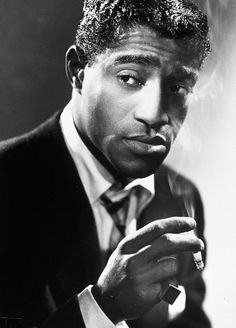
\includegraphics[width=\linewidth]{/Users/Nathaniel/Dropbox/Git/YaRrr_Book/media/sammy.jpg}
\caption{The great Sammy Davis Jr. Do yourself a favor and spend an evening watching videos of him performing on YouTube. Image used entirely without permission.}
\label{fig:sammy}
\end{marginfigure}

Plotting in R works like putting paint on a canvas. You start by creating a canvas and plotting the main elements using a \textit{high-level} plotting command. In these high-level plotting commands, you specify things like the x and y coordinates of the plot, the plot titles, and the main data in the plot. Next, you use \textit{low-level} plotting commands to sequentially add as many additional individual elements as you'd like, from lines to arrows to text. Once you are done, you can export the plot as a jpg or pdf file. In the next section, we'll cover the most common high-level plotting functions


\section{High-level plotting functions}

The most common high-level plotting function is \texttt{plot(x, y)}. While its name sounds like it can make any kind of plot, the \texttt{plot()} command creates a scatterplot from two vectors x and y:
\marginnote{\texttt{plot(x, y)}: Create a scatterplot from two vectors x and y.\\ \texttt{main}: Title of plot \\ \texttt{xlab, ylab}: axes labels \\ \texttt{xlim, ylim}: Limits of axes \\ \texttt{xaxt, yaxt}: Set to \texttt{"n"} to remove the axes \\ \texttt{cex}: Size of the plotting points \\ \texttt{pch}: Type of plotting points (see \texttt{?points})}




\vspace{5mm} %5mm vertical space
\noindent
\setlength{\fboxrule}{1.5pt}
\fbox{
\parbox{\textwidth}{

\newfun{plot()}\index{plot()}

\hline

\begin{description}

  \item[\tt{x, y}] \hfill \\
  Two vectors of data on the x and y-axes
    \item[\tt{main}] \hfill \\
 The title of the plot
    \item[\tt{xlab, ylab}] \hfill \\
  Labels for the x and y-axes.
    \item[\tt{xlim, ylim}] \hfill \\
 A vector of length two containing the minimum and maximum values of the x and y-axes. For example: \texttt{xlim = c(0, 100), ylim = c(50, 60)} will set the x limits to [0, 100] and the ylimitx to [50, 60].
    \item[\tt{col}] \hfill \\
    The color of the plotting points. For example \texttt{col = "red"} will create red plotting points.
\item[\tt{pch}] \hfill \\
    An integer indicating the type of plotting symbols (see \texttt{?points} and section below), or a string specifying symbols as text.
\item[\tt{cex}] \hfill \\
  The size of the symbols (from 0 to Inf). The default size is 1.
\item[\tt{type}] \hfill \\
The type of plot. Use \texttt{"p"} for points (the default), \texttt{"l"} for lines, \texttt{"b"} for points and lines, and \texttt{"\textbackslash n"} for no plotting


\end{description}

}
}
\vspace{5mm} %5mm vertical space


The \texttt{plot()} function, like many plotting functions, has several optional arguments that allow you to change aspects of the plot. There are so many ways to customize the look of a plot that the number of optional arguments can be overwhelming at first. Let's start by looking at an example of a simple scatterplot showing ten data points: [1, 1], [2, 2] ... [10, 10].

\begin{footnotesize}
\begin{knitrout}
\definecolor{shadecolor}{rgb}{0.969, 0.969, 0.969}\color{fgcolor}\begin{kframe}
\begin{alltt}
\hlkwd{plot}\hlstd{(}\hlkwc{x} \hlstd{=} \hlnum{1}\hlopt{:}\hlnum{10}\hlstd{,}
     \hlkwc{y} \hlstd{=} \hlnum{1}\hlopt{:}\hlnum{10}\hlstd{,}
     \hlkwc{main} \hlstd{=} \hlstr{"My First Plot"}\hlstd{,}
     \hlkwc{xlab} \hlstd{=} \hlstr{"This is the x-axis label"}\hlstd{,}
     \hlkwc{ylab} \hlstd{=} \hlstr{"This is the y-axis label"}\hlstd{,}
     \hlkwc{xlim} \hlstd{=} \hlkwd{c}\hlstd{(}\hlnum{0}\hlstd{,} \hlnum{11}\hlstd{),} \hlcom{# Min and max values for x-axis}
     \hlkwc{ylim} \hlstd{=} \hlkwd{c}\hlstd{(}\hlnum{0}\hlstd{,} \hlnum{11}\hlstd{),} \hlcom{# Min and max values for y-axis}
     \hlkwc{col} \hlstd{=} \hlstr{"blue"}\hlstd{,} \hlcom{# Color of the points}
     \hlkwc{pch} \hlstd{=} \hlnum{16}\hlstd{,} \hlcom{# Type of symbol (Filled circle)}
     \hlkwc{cex} \hlstd{=} \hlnum{1}\hlstd{,} \hlcom{# Size of the symbols,}
     \hlkwc{type} \hlstd{=} \hlstr{"p"} \hlcom{# Plot}
     \hlstd{)}
\end{alltt}
\end{kframe}

{\centering 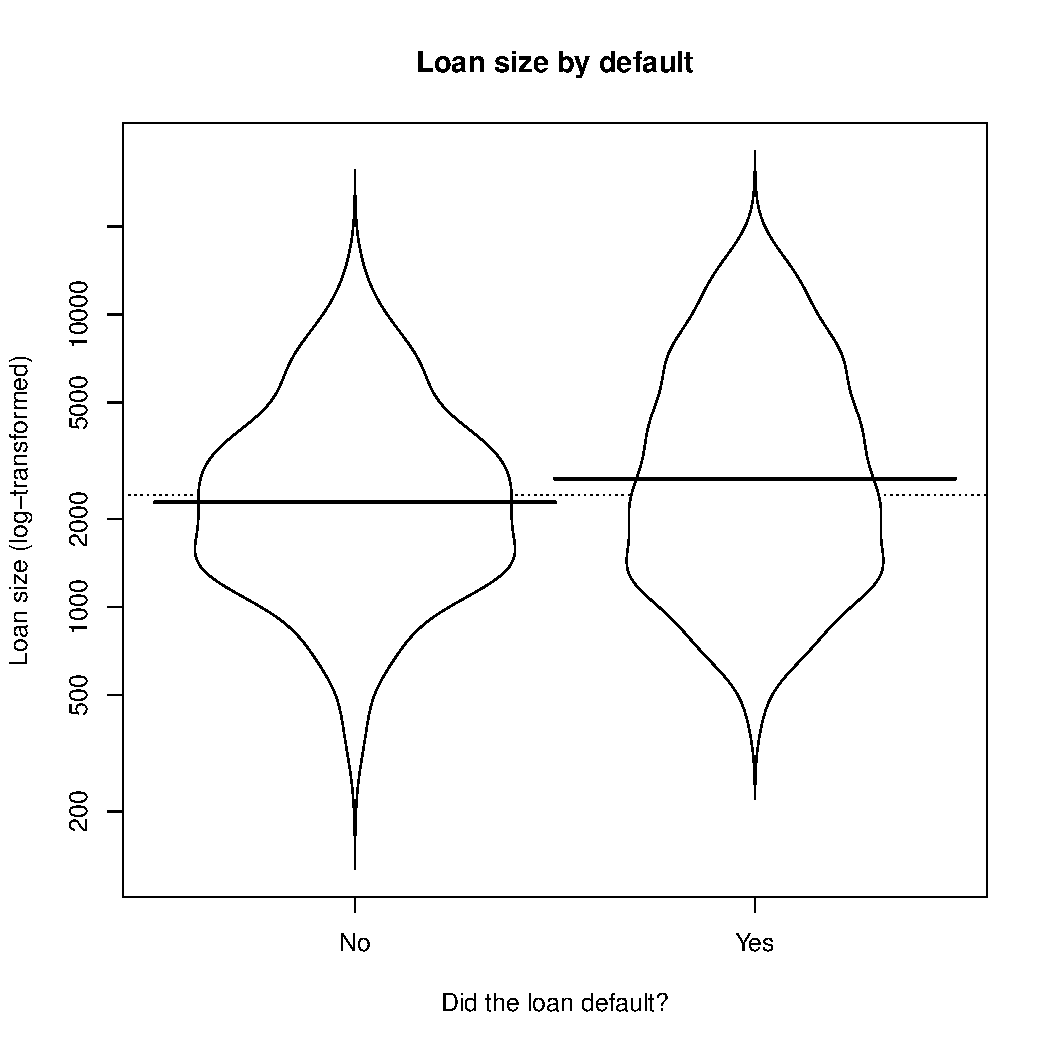
\includegraphics[width=\maxwidth]{figure/unnamed-chunk-139-1} 

}



\end{knitrout}
\end{footnotesize}


Aside from the x and y arguments, all of the arguments are optional. If you don't specify a specific argument, then R will use a default value, or try to come up with a value that makes sense. For example, if you don't specify the \texttt{xlim} and \texttt{ylim} arguments, R will set the limits so that all the points fit inside the plot.

\section{Symbol types: pch}

When you create a plot with \texttt{plot(x, y)}, you can specify the type of symbol with the \texttt{pch} argument. You can specify the symbol type in one of two ways: with an integer, or with a string. If you use a string (like \texttt{"p"}), R will use that text as the plotting symbol. If you use an integer value, you'll get the symbol that correspond to that number. See Figure~\ref{fig:pchplot} in the margin.

\begin{marginfigure}
\begin{tiny}
\begin{knitrout}
\definecolor{shadecolor}{rgb}{0.969, 0.969, 0.969}\color{fgcolor}\begin{kframe}
\begin{alltt}
\hlkwd{par}\hlstd{(}\hlkwc{mar}  \hlstd{=} \hlkwd{rep}\hlstd{(}\hlnum{0}\hlstd{,} \hlnum{4}\hlstd{))}

\hlkwd{plot}\hlstd{(}\hlkwc{x} \hlstd{=} \hlkwd{rep}\hlstd{(}\hlnum{1}\hlopt{:}\hlnum{5}\hlstd{,} \hlkwc{each} \hlstd{=} \hlnum{5}\hlstd{),}
     \hlkwc{y} \hlstd{=} \hlkwd{rep}\hlstd{(}\hlnum{5}\hlopt{:}\hlnum{1}\hlstd{,} \hlkwc{times} \hlstd{=} \hlnum{5}\hlstd{),}
     \hlkwc{pch} \hlstd{=} \hlnum{1}\hlopt{:}\hlnum{25}\hlstd{,}
     \hlkwc{xlab} \hlstd{=} \hlstr{""}\hlstd{,} \hlkwc{ylab} \hlstd{=} \hlstr{""}\hlstd{,} \hlkwc{xaxt} \hlstd{=} \hlstr{"n"}\hlstd{,} \hlkwc{yaxt} \hlstd{=} \hlstr{"n"}\hlstd{,}
     \hlkwc{xlim} \hlstd{=} \hlkwd{c}\hlstd{(}\hlnum{.5}\hlstd{,} \hlnum{5.5}\hlstd{),}
     \hlkwc{ylim} \hlstd{=} \hlkwd{c}\hlstd{(}\hlnum{0}\hlstd{,} \hlnum{6}\hlstd{),}
     \hlkwc{bty} \hlstd{=} \hlstr{"n"}\hlstd{,} \hlkwc{bg} \hlstd{=} \hlstr{"gray"}\hlstd{,} \hlkwc{cex} \hlstd{=} \hlnum{1.4}
     \hlstd{)}

\hlkwd{text}\hlstd{(}\hlkwc{x} \hlstd{=} \hlkwd{rep}\hlstd{(}\hlnum{1}\hlopt{:}\hlnum{5}\hlstd{,} \hlkwc{each} \hlstd{=} \hlnum{5}\hlstd{)} \hlopt{-} \hlnum{.35}\hlstd{,}
     \hlkwc{y} \hlstd{=} \hlkwd{rep}\hlstd{(}\hlnum{5}\hlopt{:}\hlnum{1}\hlstd{,} \hlkwc{times} \hlstd{=} \hlnum{5}\hlstd{),}
     \hlkwc{labels} \hlstd{=} \hlnum{1}\hlopt{:}\hlnum{25}\hlstd{,} \hlkwc{cex} \hlstd{=} \hlnum{1.2}
     \hlstd{)}
\end{alltt}
\end{kframe}
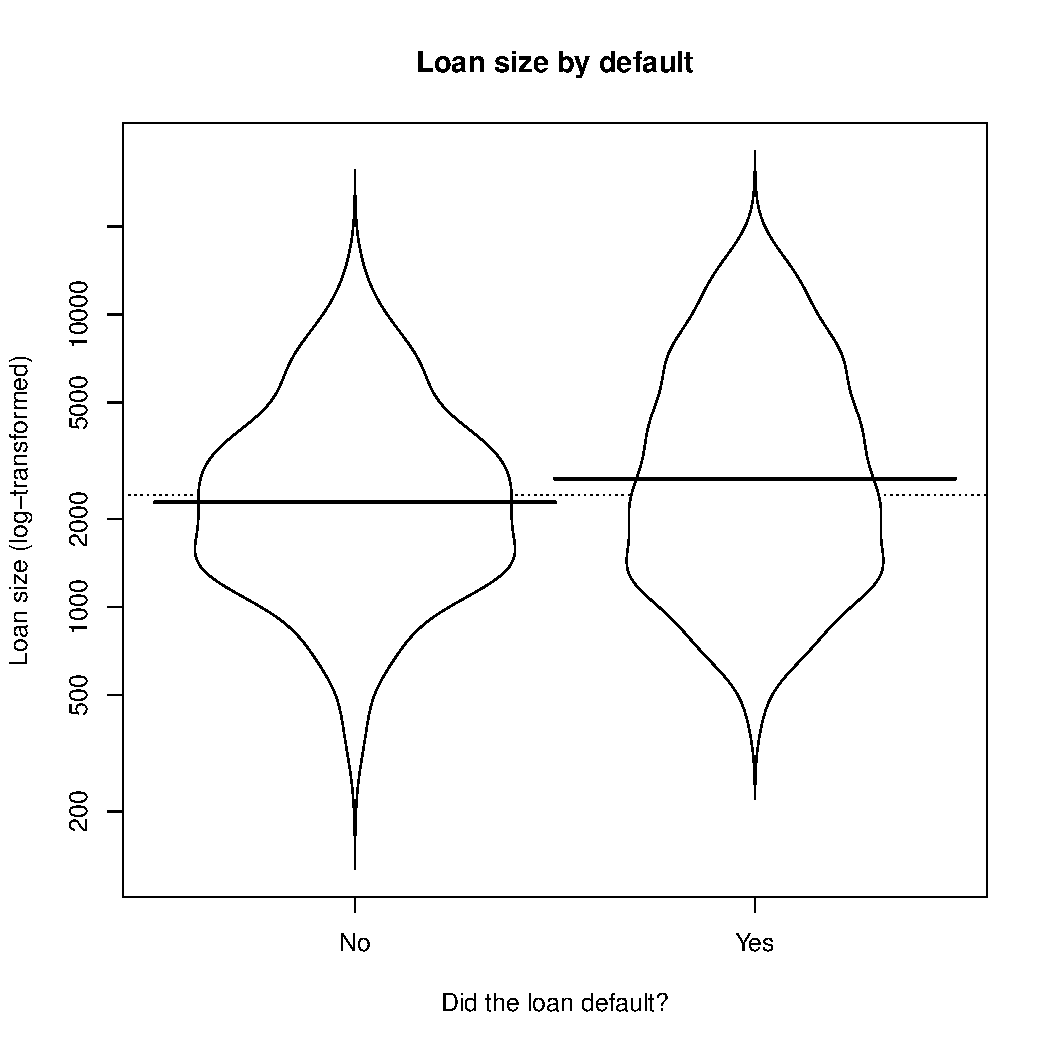
\includegraphics[width=\maxwidth]{figure/unnamed-chunk-140-1} 

\end{knitrout}
\end{tiny}
\caption{The symbol types associated with the \texttt{pch} plotting parameter.}
\label{fig:pchplot}
\end{marginfigure}

Symbols differ in their border shape and how the filling is done. Symbols 1 through 14 only have borders and are always empty, while symbols 15 through 20 don't have a border and are always filled. Symbols 21 through 25 have both a border and a filling.

To specify the border color for all symbols, use the \texttt{col} argument. For symbols 21 through 25, you can additionally set the color of the fill using the \texttt{bg} ("background") argument.


\section{Other high-Level plotting commands}

While \texttt{plot()} is the most widely used high-level plotting command, there are several (perhaps even hundreds) of additional ones. I'll briefly highlight a few additional ones that you may wish to use

\subsection{Histograms \texttt{hist()}}

\begin{marginfigure}
\begin{knitrout}
\definecolor{shadecolor}{rgb}{0.969, 0.969, 0.969}\color{fgcolor}\begin{kframe}
\begin{alltt}
\hlkwd{hist}\hlstd{(}\hlkwc{x} \hlstd{= ChickWeight}\hlopt{$}\hlstd{weight,}
     \hlkwc{main} \hlstd{=} \hlstr{"Chick Weights"}\hlstd{,}
     \hlkwc{xlab} \hlstd{=} \hlstr{"Weights (all time points"}
     \hlstd{)}
\end{alltt}
\end{kframe}
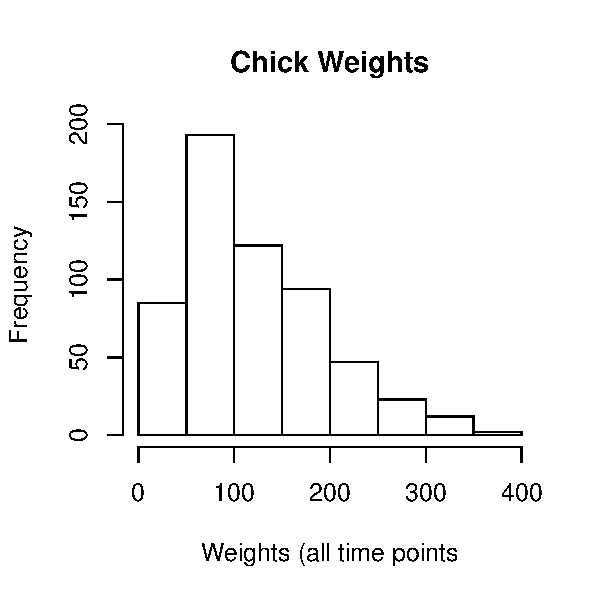
\includegraphics[width=\maxwidth]{figure/unnamed-chunk-141-1} 

\end{knitrout}
\caption{Histogram of weight data from \texttt{ChickWeight}}
\label{fig:histogram}
\end{marginfigure}

The function \texttt{hist()} is a high-level plotting command that creates (wait for it...) a histogram. Here are the main arguments for \texttt{hist()}:



\vspace{5mm} %5mm vertical space
\noindent
\setlength{\fboxrule}{1.5pt}
\fbox{
\parbox{\textwidth}{

\newfun{hist()}\index{hist()}

\hline

\begin{description}

  \item[\tt{x}] \hfill \\
  A vector of data
    \item[\tt{breaks}] \hfill \\
 One of several values that defines how bins are created. The most common argument is a single number giving the number of bins you want in the histogram. See \texttt{?hist} for additional ways to specify this.
    \item[\tt{col}] \hfill \\
    The color of the filling of the bars. (e.g.; \texttt{col = "red"})
    \item[\tt{border}] \hfill \\
   The color of the border of the bars. (e.g.; \texttt{border = "green"})
    \item[\tt{probability}] \hfill \\
A logical value indicating whether to plot the results as probabilities (the default is FALSE)
\item[\tt{main, xlab, ylab, xlim, ylim ...}] \hfill \\
    Other standard plotting arguments

\end{description}

}
}
\vspace{5mm} %5mm vertical space


You can see an example of a histogram in the margin Figure~\ref{fig:histogram}.

\subsection{Boxplots \texttt{boxplot()}}

Boxplots aren't used so often anymore (for reasons that I'll show you shortly), but I think it's good to know how to make them, even if it's just for historical purposes. To create a boxplot, use the \texttt{boxplot()} function:


\begin{marginfigure}
\begin{tiny}
\begin{knitrout}
\definecolor{shadecolor}{rgb}{0.969, 0.969, 0.969}\color{fgcolor}\begin{kframe}
\begin{alltt}
\hlkwd{boxplot}\hlstd{(}\hlkwc{x} \hlstd{= ChickWeight}\hlopt{$}\hlstd{weight,}
        \hlkwc{names} \hlstd{=} \hlstr{"All Data"}\hlstd{,} \hlkwc{ylab} \hlstd{=} \hlstr{"Weight"}\hlstd{,}
        \hlkwc{main} \hlstd{=} \hlstr{"Plot 1: All Weights"}\hlstd{)}
\end{alltt}
\end{kframe}
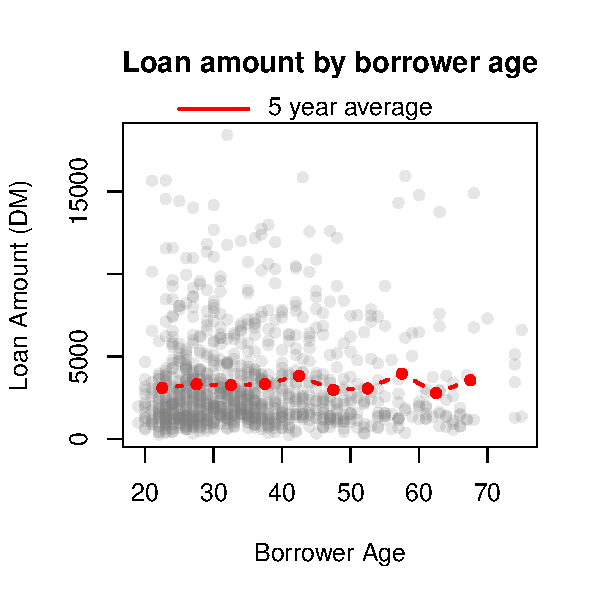
\includegraphics[width=\maxwidth]{figure/unnamed-chunk-142-1} 

\end{knitrout}
\end{tiny}
\caption{Plotting data from a single vector}
\label{fig:boxplot1}
\end{marginfigure}

\begin{marginfigure}
\begin{tiny}
boxplot(weight ~ Diet, # Formula: DV is weight and IV is Diet
        data = ChickWeight, # dataframe
        xlab = "Diet", ylab = "Weight", 
        main = "Plot 2: Weight separated by Diet")
@
\end{tiny}
\caption{Plotting data as a function of levels of an independent variable using the \texttt{y {\raise.17ex\hbox{$\scriptstyle\sim$}} x} formula notation.}
\label{fig:boxplot2}
\end{marginfigure}



\vspace{5mm} %5mm vertical space
\noindent
\setlength{\fboxrule}{1.5pt}
\fbox{
\parbox{\textwidth}{

\newfun{boxplot()}\index{boxplot()}

\hline

\begin{description}

  \item[\tt{formula, data}] \hfill \\
      A formula in the form \texttt{formula = dv {\raise.17ex\hbox{$\scriptstyle\sim$}} iv} indicating the dependent variable and independent variable, and a dataframe containing the variables in the formula. For example \texttt{formula = height {\raise.17ex\hbox{$\scriptstyle\sim$}} sex}
        \item[\tt{subset}] \hfill \\
  An optional logical vector indicating a subset of the data to plot. For example, the command \texttt{subset = gender == "male" \& weight < 120}, will only plot data for males with weight less than 120.
         \item[\tt{border, col}] \hfill \\
    The color of the borders (\texttt{border}) and filling (\texttt{col}) of the boxes.
        \item[\tt{names}] \hfill \\
      A string vector indicating the names of the boxes. E.g.; \texttt{names = c("males", "females")}
        \item[\tt{horizontal}] \hfill \\
   A logical value indicating whether to plot the boxes horizontally.
\end{description}

}
}
\vspace{5mm} %5mm vertical space



When you use \texttt{boxplot()}, you can either specify a single vector of data to plot, or you can use a \texttt{formula} to indicate a dependent and independent variable. If you do this, R will add separate boxes for all values of the independent variable.

Let's go through two examples of boxplots in Figure~\ref{fig:boxplot}. In the first plot, I just entered a single vector of data: \texttt{ChickWeight\$weight} representing all weight data in the dataframe. In the second plot, I plotted separate boxes for the different levels of \texttt{Diet} using the formula notation \texttt{weight {\raise.17ex\hbox{$\scriptstyle\sim$}} Diet}. If you're wondering how R knows that I'm referring to the \texttt{ChickWeight} dataframe when using the formula notation, the answer is that I had to specify the name of the dataframe \texttt{ChickWeight} as an additional \texttt{data} argument. This argument tells R that the objects in the formula are names in the \texttt{ChickWeight} dataframe.



\subsection{Beanplots: \texttt{beanplot()}}

\begin{marginfigure}
\begin{tiny}
\begin{knitrout}
\definecolor{shadecolor}{rgb}{0.969, 0.969, 0.969}\color{fgcolor}\begin{kframe}
\begin{alltt}
\hlkwd{require}\hlstd{(}\hlstr{"beanplot"}\hlstd{)}

\hlstd{bean.cols} \hlkwb{<-} \hlkwd{lapply}\hlstd{(}\hlkwd{brewer.pal}\hlstd{(}\hlnum{4}\hlstd{,} \hlstr{"Set3"}\hlstd{),}
                    \hlkwa{function}\hlstd{(}\hlkwc{x}\hlstd{) \{}\hlkwd{return}\hlstd{(}\hlkwd{c}\hlstd{(x,} \hlstr{"black"}\hlstd{,} \hlstr{"black"}\hlstd{,} \hlstr{"black"}\hlstd{))\})}

\hlkwd{beanplot}\hlstd{(weight} \hlopt{~} \hlstd{Diet,}
         \hlkwc{data} \hlstd{= ChickWeight,}
         \hlkwc{main} \hlstd{=} \hlstr{"Beans"}\hlstd{,}
         \hlkwc{xlab} \hlstd{=} \hlstr{"Diet"}\hlstd{,}
         \hlkwc{ylab} \hlstd{=} \hlstr{"Weight"}\hlstd{,}
         \hlkwc{col} \hlstd{= bean.cols ,}
         \hlkwc{lwd} \hlstd{=} \hlnum{1}\hlstd{,}
         \hlkwc{what} \hlstd{=} \hlkwd{c}\hlstd{(}\hlnum{1}\hlstd{,} \hlnum{1}\hlstd{,} \hlnum{1}\hlstd{,} \hlnum{1}\hlstd{),} \hlkwc{log} \hlstd{=} \hlstr{""}
         \hlstd{)}
\end{alltt}
\end{kframe}
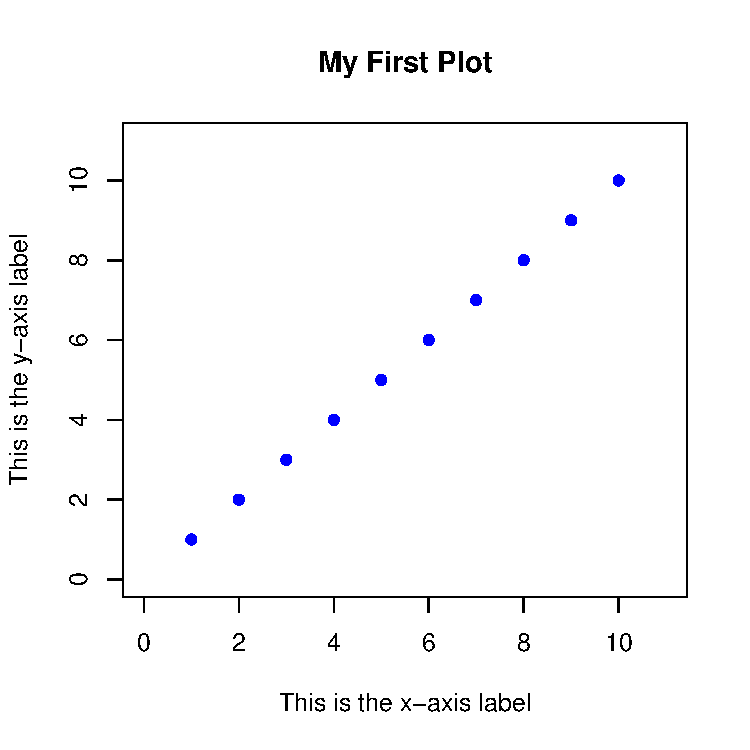
\includegraphics[width=\maxwidth]{figure/unnamed-chunk-143-1} 

\end{knitrout}
\end{tiny}
\caption{Beanplots from the \texttt{beanplot} package. Beanplots are great at simultaneously showing raw data, smoothed distributions, and group averages.}
\label{fig:beanplot}
\end{marginfigure}

The last high-level plotting I want to show you is the \texttt{beanplot()} function. This function creates a beanplot, which (like boxplots and histograms), shows you a distribution of sample data. However, as you can see in Figure~\ref{fig:beanplot}, they look much, much cooler than a boxplot or histogram. What's really great about beanplots is that they show you a combination of three elements: raw data, smoothed distribution lines, and group averages. This means that you can quickly detect outliers, multiple modes, or missing data much better than you can with boxplots.

To use the \texttt{beanplot()} function, you first need to download the \texttt{beanplot} package:

\begin{footnotesize}
\begin{knitrout}
\definecolor{shadecolor}{rgb}{0.969, 0.969, 0.969}\color{fgcolor}\begin{kframe}
\begin{alltt}
\hlkwd{install.packages}\hlstd{(}\hlstr{"beanplot"}\hlstd{)}
\end{alltt}
\end{kframe}
\end{knitrout}
\end{footnotesize}

Here are some of the main arguments for \texttt{beanplot()}. Check out the help menu (\texttt{?beanplot}) to see several additional arguments


\vspace{5mm} %5mm vertical space
\noindent
\setlength{\fboxrule}{1.5pt}
\fbox{
\parbox{\textwidth}{

\newfun{beanplot()}\index{beanplot()}

\hline

\begin{description}

  \item[\tt{formula, data}] \hfill \\
      A formula in the form \texttt{formula = dv {\raise.17ex\hbox{$\scriptstyle\sim$}} iv} indicating the dependent variable and independent variable, and a dataframe containing the variables in the formula. For example \texttt{formula = height {\raise.17ex\hbox{$\scriptstyle\sim$}} sex, data = survey}
        \item[\tt{subset}] \hfill \\
  An optional logical vector indicating a subset of the data to plot. For example, the command \texttt{subset = gender == "male" \& weight < 120}, will only plot data for males with weight less than 120.
         \item[\tt{what}] \hfill \\
A vector of four boolean (0 or 1) values indicating what to plot in the following order: the total average line, the beans, the bean average, and the beanlines. For example, to plot everything, use \texttt{what = c(1, 1, 1, 1)}. To plot just the beans, use \texttt{what = c(0, 0, 1, 0)}
        \item[\tt{color}] \hfill \\
    The colors in the plot. A vector of up to four colors can be used representing the areas of the beans, the lines inside the beans, the lines outside the beans, and the average line per bean. If you want to make each bean a different color, you have to specify a list of separate color vectors, one for each bean. Look at my code in Figure~\ref{fig:beanplot} for a way to do this using \texttt{lapply}.
        \item[\tt{names}] \hfill \\
A vector of names of the beans.
\item[\tt{overallline}] \hfill \\
A method for determining the overall line (either \texttt{"mean"}or \texttt{"median"})
\end{description}

}
}
\vspace{5mm} %5mm vertical space

The code for creating beanplots is very similar to the code for boxplots. The following code creates the plot in Figure~\ref{fig:beanplot}. 

\begin{footnotesize}
\begin{knitrout}
\definecolor{shadecolor}{rgb}{0.969, 0.969, 0.969}\color{fgcolor}\begin{kframe}
\begin{alltt}
\hlkwd{require}\hlstd{(}\hlstr{"beanplot"}\hlstd{)}
\hlstd{bean.cols} \hlkwb{<-} \hlkwd{lapply}\hlstd{(}\hlkwd{brewer.pal}\hlstd{(}\hlnum{4}\hlstd{,} \hlstr{"Set3"}\hlstd{),}
                    \hlkwa{function}\hlstd{(}\hlkwc{x}\hlstd{) \{}\hlkwd{return}\hlstd{(}\hlkwd{c}\hlstd{(x,} \hlstr{"black"}\hlstd{,} \hlstr{"black"}\hlstd{,} \hlstr{"black"}\hlstd{))\})}

\hlkwd{beanplot}\hlstd{(weight} \hlopt{~} \hlstd{Diet,}
         \hlkwc{data} \hlstd{= ChickWeight,}
         \hlkwc{main} \hlstd{=} \hlstr{"Beans"}\hlstd{,}
         \hlkwc{xlab} \hlstd{=} \hlstr{"Diet"}\hlstd{,}
         \hlkwc{ylab} \hlstd{=} \hlstr{"Weight"}\hlstd{,}
         \hlkwc{col} \hlstd{= bean.cols ,}
         \hlkwc{lwd} \hlstd{=} \hlnum{1}\hlstd{,}
         \hlkwc{what} \hlstd{=} \hlkwd{c}\hlstd{(}\hlnum{1}\hlstd{,} \hlnum{1}\hlstd{,} \hlnum{1}\hlstd{,} \hlnum{1}\hlstd{),} \hlkwc{log} \hlstd{=} \hlstr{""}
         \hlstd{)}
\end{alltt}
\end{kframe}
\end{knitrout}
\end{footnotesize}

One major new argument is \texttt{what}, which dictates what exactly is plotted. You specify \texttt{what} using a vector of four Boolean (0 or 1) values. In the plot in Figure~\ref{fig:beanplot}, I've set all values to 1 which means that the function will include all four plot elements. If you'd like to remove certain elements, like the individual lines or the average lines, you can remove them by replacing the respective 1s to 0s.





\section{Low-level plotting functions}

Once you've created a plot with a high-level plotting function, you can add additional elements, like additional data points, reference lines, text, and legends using low-level plotting functions. There are many low-level plotting functions, I will focus on those that I frequently use.

\subsection{Starting with a blank plot}


\begin{marginfigure}
\begin{tiny}
\begin{knitrout}
\definecolor{shadecolor}{rgb}{0.969, 0.969, 0.969}\color{fgcolor}\begin{kframe}
\begin{alltt}
\hlcom{# Create a blank plot}
\hlkwd{plot}\hlstd{(}\hlkwc{x} \hlstd{=} \hlnum{1}\hlstd{,} \hlkwc{y} \hlstd{=} \hlnum{1}\hlstd{,} \hlkwc{xlab} \hlstd{=} \hlstr{""}\hlstd{,} \hlkwc{ylab} \hlstd{=} \hlstr{""}\hlstd{,}
     \hlkwc{xaxt} \hlstd{=} \hlstr{"n"}\hlstd{,} \hlkwc{yaxt} \hlstd{=} \hlstr{"n"}\hlstd{,} \hlkwc{type} \hlstd{=} \hlstr{"n"}\hlstd{,}
     \hlkwc{xlim} \hlstd{=} \hlkwd{c}\hlstd{(}\hlnum{0}\hlstd{,} \hlnum{100}\hlstd{),} \hlkwc{ylim} \hlstd{=} \hlkwd{c}\hlstd{(}\hlnum{0}\hlstd{,} \hlnum{100}\hlstd{),} \hlkwc{main} \hlstd{=} \hlstr{"Blank Plot"}\hlstd{)}
\end{alltt}
\end{kframe}
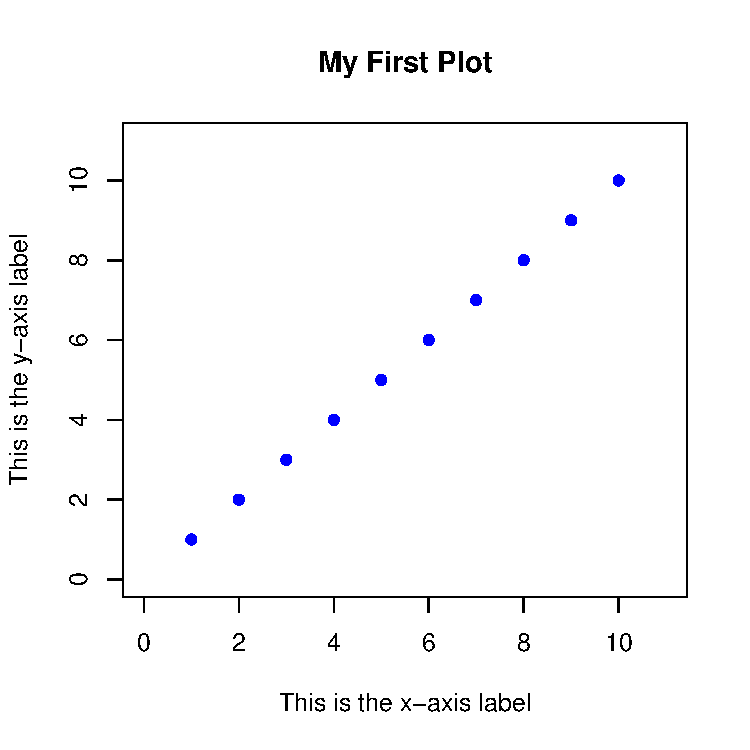
\includegraphics[width=\maxwidth]{figure/unnamed-chunk-146-1} 

\end{knitrout}
\end{tiny}
\caption{A blank plot. Useful to start with before adding elements with low-level plotting commands. Just make sure to set the axis limits to values that make sense for your future data.}
\label{fig:blankplot}
\end{marginfigure}

I like using low-level plotting functions so much that I frequently like to start with a (mostly) blank plotting space, and then add the main plot elements using low-level plotting functions. To start with a blank plot, use the \texttt{plot()} function combined with the arguments \texttt{type = "n", xaxt = "n", yaxt = "n"} and all labels set to \texttt{""}. See margin Figure~\ref{fig:blankplot} for an example

Once you've created a blank plot, you can proceed to add all the elements you'd like with low-level plotting commands. Let's start with \texttt{points()}, which adds points to an existing plot

\subsection{points()}


\begin{marginfigure}
\begin{tiny}
\begin{knitrout}
\definecolor{shadecolor}{rgb}{0.969, 0.969, 0.969}\color{fgcolor}\begin{kframe}
\begin{alltt}
\hlcom{# Get subsets of data}
\hlstd{diet.1} \hlkwb{<-} \hlkwd{subset}\hlstd{(ChickWeight, Diet} \hlopt{==} \hlnum{1}\hlstd{)}
\hlstd{diet.2} \hlkwb{<-} \hlkwd{subset}\hlstd{(ChickWeight, Diet} \hlopt{==} \hlnum{2}\hlstd{)}

\hlcom{# Create a blank plot}
\hlkwd{plot}\hlstd{(}\hlkwc{x} \hlstd{=} \hlnum{1}\hlstd{,} \hlkwc{y} \hlstd{=} \hlnum{1}\hlstd{,} \hlkwc{xlab} \hlstd{=} \hlstr{"Time"}\hlstd{,} \hlkwc{ylab} \hlstd{=} \hlstr{"Weight"}\hlstd{,}
     \hlkwc{type} \hlstd{=} \hlstr{"n"}\hlstd{,} \hlkwc{main} \hlstd{=} \hlstr{"Even More Chicken Weights"}\hlstd{,}
     \hlkwc{xlim} \hlstd{=} \hlkwd{c}\hlstd{(}\hlnum{0}\hlstd{,} \hlnum{23}\hlstd{),} \hlkwc{ylim} \hlstd{=} \hlkwd{c}\hlstd{(}\hlnum{0}\hlstd{,} \hlnum{315}\hlstd{))}

\hlcom{# Add red points for diet 1}
\hlkwd{points}\hlstd{(diet.1}\hlopt{$}\hlstd{Time, diet.1}\hlopt{$}\hlstd{weight,} \hlkwc{pch} \hlstd{=} \hlnum{16}\hlstd{,} \hlkwc{col} \hlstd{=} \hlstr{"red"}\hlstd{)}

\hlcom{# Add skyblue points for diet 2}
\hlkwd{points}\hlstd{(diet.2}\hlopt{$}\hlstd{Time, diet.2}\hlopt{$}\hlstd{weight,} \hlkwc{pch} \hlstd{=} \hlnum{16}\hlstd{,} \hlkwc{col} \hlstd{=} \hlstr{"skyblue"}\hlstd{)}
\end{alltt}
\end{kframe}
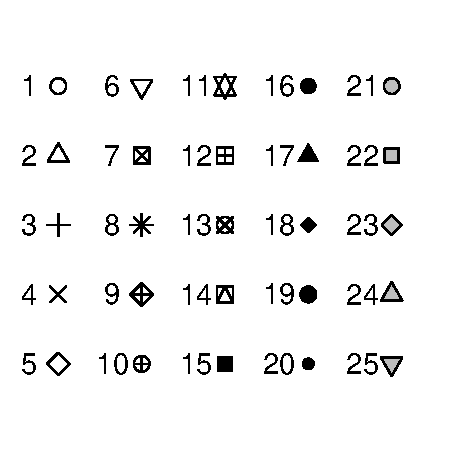
\includegraphics[width=\maxwidth]{figure/unnamed-chunk-147-1} 

\end{knitrout}
\caption{Adding additional points to an existing plot with points()}
\label{pointsexample}
\end{tiny}
\end{marginfigure}


\vspace{5mm} %5mm vertical space
\noindent
\setlength{\fboxrule}{1.5pt}
\fbox{
\parbox{\textwidth}{

\newfun{points()}\index{points()}

\hline

\begin{description}

\item[\tt{x, y}] \hfill \\
Two vectors corresponding to the x and y values of the points

\item[\tt{pch, col, bg}] \hfill \\
Type of plotting symols (\texttt{pch}), color of the plotting symbols (\texttt{col}), and the color of the filling of the plotting symbols ((\texttt{bg})) for plotting symbols 21 through 25
  
  
\end{description}

}
}
\vspace{5mm} %5mm vertical space


For example, to add red circle points to a plot where \texttt{x.vals} are the x-values and \texttt{y.vals} are the y.values, you can run the code:

\begin{knitrout}
\definecolor{shadecolor}{rgb}{0.969, 0.969, 0.969}\color{fgcolor}\begin{kframe}
\begin{alltt}
\hlkwd{points}\hlstd{(}\hlkwc{x} \hlstd{= x.vals,} \hlcom{# x-values}
       \hlkwc{y} \hlstd{= y.vals,} \hlcom{# y-values}
       \hlkwc{col} \hlstd{=} \hlstr{"red"}\hlstd{,} \hlcom{# Symbol color}
       \hlkwc{pch} \hlstd{=} \hlnum{16} \hlcom{# Symbol type (circles)}
       \hlstd{)}
\end{alltt}
\end{kframe}
\end{knitrout}

Because you can continue adding as many low-level plotting commands to a plot as you'd like, you can keep adding different types or colors of points by adding additional \texttt{points()} functions. However, keep in mind that because R plots each element on top of the previous one, early calls to \texttt{points()} might be covered by later calls. So add the points that you want in the foreground at the end!

In margin Figure~\ref{pointsexample}, I use the points function to plot data from ChickWeight, where chicks on diet 1 are plotted in red, and chicks on diet 2 are plotted in skyblue.

Next, we'll look at \texttt{abline()} which adds straight lines to a plot:


\subsection{abline()}

\begin{marginfigure}
\begin{tiny}
\begin{knitrout}
\definecolor{shadecolor}{rgb}{0.969, 0.969, 0.969}\color{fgcolor}\begin{kframe}
\begin{alltt}
\hlkwd{par}\hlstd{(}\hlkwc{mar} \hlstd{=} \hlkwd{c}\hlstd{(}\hlnum{3}\hlstd{,} \hlnum{0}\hlstd{,} \hlnum{6}\hlstd{,} \hlnum{0}\hlstd{))}
\hlkwd{plot}\hlstd{(}\hlnum{1}\hlstd{,} \hlkwc{xlim} \hlstd{=} \hlkwd{c}\hlstd{(}\hlnum{0}\hlstd{,} \hlnum{7}\hlstd{),} \hlkwc{ylim} \hlstd{=} \hlkwd{c}\hlstd{(}\hlnum{0}\hlstd{,} \hlnum{1}\hlstd{),}
     \hlkwc{type} \hlstd{=} \hlstr{"n"}\hlstd{,} \hlkwc{xlab} \hlstd{=} \hlstr{"lty values"}\hlstd{,} \hlkwc{ylab} \hlstd{=} \hlstr{""}\hlstd{,}
     \hlkwc{xaxt} \hlstd{=} \hlstr{"n"}\hlstd{,} \hlkwc{yaxt} \hlstd{=} \hlstr{"n"}\hlstd{,} \hlkwc{bty} \hlstd{=} \hlstr{"n"}\hlstd{,} \hlkwc{main} \hlstd{=} \hlstr{""}\hlstd{)}

\hlkwd{abline}\hlstd{(}\hlkwc{v} \hlstd{=} \hlnum{1}\hlopt{:}\hlnum{6}\hlstd{,} \hlkwc{lty} \hlstd{=} \hlnum{1}\hlopt{:}\hlnum{6}\hlstd{,} \hlkwc{lwd} \hlstd{=} \hlnum{2}\hlstd{)}

\hlkwd{mtext}\hlstd{(}\hlnum{1}\hlopt{:}\hlnum{6}\hlstd{,}
      \hlkwc{side} \hlstd{=} \hlnum{3}\hlstd{,}
      \hlkwc{at} \hlstd{=} \hlnum{1}\hlopt{:}\hlnum{6}\hlstd{,} \hlkwc{cex} \hlstd{=} \hlnum{1.5}\hlstd{,} \hlkwc{line} \hlstd{=} \hlnum{1}
      \hlstd{)}

\hlkwd{mtext}\hlstd{(}\hlstr{"lty = ..."}\hlstd{,} \hlkwc{side} \hlstd{=} \hlnum{3}\hlstd{,} \hlkwc{at} \hlstd{=} \hlnum{3.5}\hlstd{,} \hlkwc{line} \hlstd{=} \hlnum{4}\hlstd{,} \hlkwc{cex} \hlstd{=} \hlnum{2}\hlstd{)}
\end{alltt}
\end{kframe}
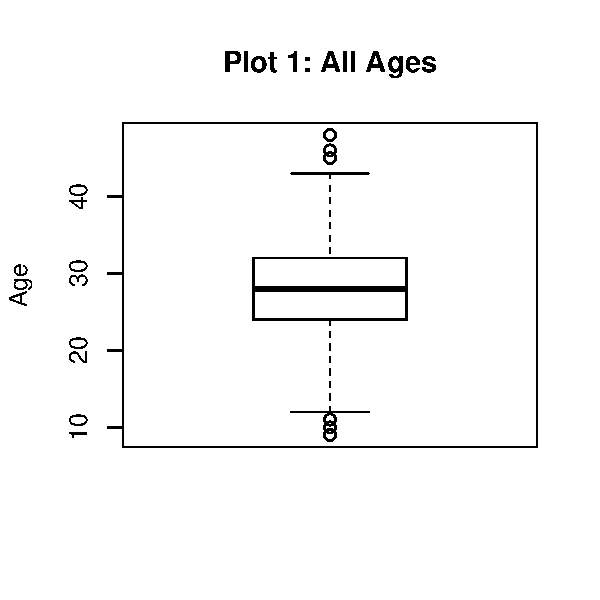
\includegraphics[width=\maxwidth]{figure/unnamed-chunk-149-1} 

\end{knitrout}
\end{tiny}
\label{fig:ltytypes}
\caption{Line types generated from arguments to lty.}
\end{marginfigure}




\vspace{5mm} %5mm vertical space
\noindent
\setlength{\fboxrule}{1.5pt}
\fbox{
\parbox{\textwidth}{

\newfun{abline()}\index{abline()}

\hline

\begin{description}

\item[\tt{a, b}] \hfill \\
Numeric scalars or vectors indicating the slope (\texttt{a}) and intercept {\texttt{b}} of the line(s)

\item[\tt{h, v}] \hfill \\
Numeric scalars or vectors indicating the y-value of horizontal lines (\texttt{h}) or x-values of vertical lines {\texttt{v}}. For example, \texttt{abline(h = 1)} will add a horizontal line at y = 1, while \texttt{abline(v = 10)} will add a vertical line at x = 1

\item[\tt{lty, lwd}] \hfill \\
Type (\texttt{lty}) and width (\texttt{lwd}) of line. See margin Figure~\ref{fig:ltytypes} to see line types.
  
\end{description}

}
}
\vspace{5mm} %5mm vertical space


For example, to add a vertical line at an x-value of 0 or a horizontal line at a y-vale at 100 you'd enter

\begin{knitrout}
\definecolor{shadecolor}{rgb}{0.969, 0.969, 0.969}\color{fgcolor}\begin{kframe}
\begin{alltt}
\hlkwd{abline}\hlstd{(}\hlkwc{v} \hlstd{=} \hlnum{0}\hlstd{)} \hlcom{# Add a vertical line at x = 0}
\hlkwd{abline}\hlstd{(}\hlkwc{h} \hlstd{=} \hlnum{100}\hlstd{)} \hlcom{# Add a horizontal line at y = 100}
\end{alltt}
\end{kframe}
\end{knitrout}

You can easily use abline() to add gridlines to plots by entering vectors in the \texttt{h} and \texttt{v} arguments. For example, to add gridlines to a plot at x-values and y-values from 0 to 10 in steps of 1, you'd enter

\begin{knitrout}
\definecolor{shadecolor}{rgb}{0.969, 0.969, 0.969}\color{fgcolor}\begin{kframe}
\begin{alltt}
\hlkwd{abline}\hlstd{(}\hlkwc{v} \hlstd{=} \hlnum{1}\hlopt{:}\hlnum{10}\hlstd{)} \hlcom{# Add vertical lines from 1 to 10}
\hlkwd{abline}\hlstd{(}\hlkwc{h} \hlstd{=} \hlnum{1}\hlopt{:}\hlnum{10}\hlstd{)} \hlcom{# Add horizontal lines from 1 to 10}
\end{alltt}
\end{kframe}
\end{knitrout}

In margin Figure~\ref{fig:gridlinesexample} I add gridlines and a diagonal reference line to a plot before adding points.

\begin{marginfigure}
\begin{tiny}
\begin{knitrout}
\definecolor{shadecolor}{rgb}{0.969, 0.969, 0.969}\color{fgcolor}\begin{kframe}
\begin{alltt}
\hlcom{# Create a blank plot}
\hlkwd{plot}\hlstd{(}\hlkwc{x} \hlstd{=} \hlnum{1}\hlstd{,} \hlkwc{y} \hlstd{=} \hlnum{1}\hlstd{,} \hlkwc{xlab} \hlstd{=} \hlstr{"Group"}\hlstd{,} \hlkwc{ylab} \hlstd{=} \hlstr{"Length"}\hlstd{,}
     \hlkwc{type} \hlstd{=} \hlstr{"n"}\hlstd{,} \hlkwc{main} \hlstd{=} \hlstr{"Gridlines with abline()"}\hlstd{,}
     \hlkwc{xlim} \hlstd{=} \hlkwd{c}\hlstd{(}\hlnum{0}\hlstd{,} \hlnum{10}\hlstd{),} \hlkwc{ylim} \hlstd{=} \hlkwd{c}\hlstd{(}\hlnum{0}\hlstd{,} \hlnum{10}\hlstd{))}

\hlcom{# Add horizontal gridlines}
\hlkwd{abline}\hlstd{(}\hlkwc{h} \hlstd{=} \hlnum{1}\hlopt{:}\hlnum{10}\hlstd{,} \hlkwc{lwd} \hlstd{=} \hlnum{1}\hlstd{,} \hlkwc{col} \hlstd{=} \hlkwd{gray}\hlstd{(}\hlnum{.8}\hlstd{))}

\hlcom{# Add vertical gridlines}
\hlkwd{abline}\hlstd{(}\hlkwc{v} \hlstd{=} \hlnum{1}\hlopt{:}\hlnum{10}\hlstd{,} \hlkwc{col} \hlstd{=} \hlkwd{gray}\hlstd{(}\hlnum{.8}\hlstd{))}

\hlcom{# Add main diagonal reference line}
\hlkwd{abline}\hlstd{(}\hlkwc{a} \hlstd{=} \hlnum{0}\hlstd{,} \hlkwc{b} \hlstd{=} \hlnum{1}\hlstd{,} \hlkwc{lwd} \hlstd{=} \hlnum{2}\hlstd{,} \hlkwc{lty} \hlstd{=} \hlnum{2}\hlstd{)}

\hlcom{# Create data}
\hlstd{x.data} \hlkwb{<-} \hlkwd{rnorm}\hlstd{(}\hlnum{100}\hlstd{,} \hlkwc{mean} \hlstd{=} \hlnum{5}\hlstd{,} \hlkwc{sd} \hlstd{=} \hlnum{2}\hlstd{)}
\hlstd{y.data} \hlkwb{<-} \hlstd{x.data} \hlopt{+} \hlkwd{rnorm}\hlstd{(}\hlnum{100}\hlstd{,} \hlkwc{mean} \hlstd{=} \hlnum{0}\hlstd{,} \hlkwc{sd} \hlstd{=} \hlnum{3}\hlstd{)}

\hlcom{# Add points}
\hlkwd{points}\hlstd{(}\hlkwc{x} \hlstd{= x.data,}
       \hlkwc{y} \hlstd{= y.data,} \hlkwc{pch} \hlstd{=} \hlnum{16}\hlstd{,}
       \hlkwc{col} \hlstd{=} \hlkwd{gray}\hlstd{(}\hlnum{.4}\hlstd{,} \hlkwc{alpha} \hlstd{=} \hlnum{.5}\hlstd{),}
       \hlkwc{cex} \hlstd{=} \hlkwd{c}\hlstd{(}\hlkwd{runif}\hlstd{(}\hlnum{90}\hlstd{,} \hlnum{0}\hlstd{,} \hlnum{2}\hlstd{),} \hlkwd{runif}\hlstd{(}\hlnum{10}\hlstd{,} \hlnum{3}\hlstd{,} \hlnum{4}\hlstd{))}
       \hlstd{)}
\end{alltt}
\end{kframe}
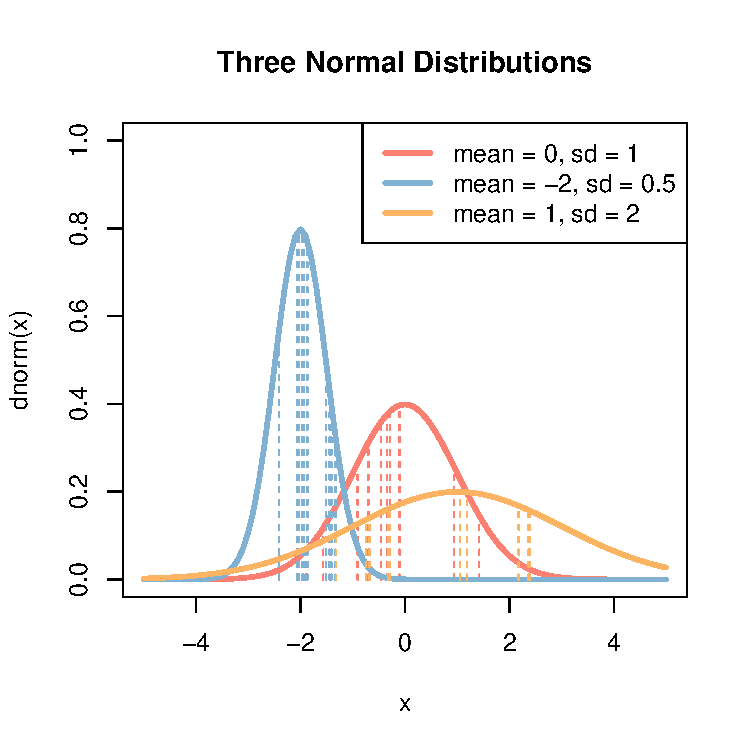
\includegraphics[width=\maxwidth]{figure/unnamed-chunk-152-1} 

\end{knitrout}
\caption{Adding gridlines to a plot with abline().}
\label{fig:gridlinesexample}
\end{tiny}
\end{marginfigure}

Next, we'll move on to \texttt{text}, which adds text to a plot

\subsection{text()}

With \texttt{text()}, you can add text to a plot. You can use text() to highlight specific points of interest in the plot, or to add information (like a third variable) for every point in a plot. Here are the main arguments to \texttt{text()}




\vspace{5mm} %5mm vertical space
\noindent
\setlength{\fboxrule}{1.5pt}
\fbox{
\parbox{\textwidth}{

\newfun{text()}\index{text()}

\hline

\begin{description}

\item[\tt{x, y}] \hfill \\
Numeric scalars or vectors specifying the coordinates of the \textt{labels}

\item[\tt{labels}] \hfill \\
String vector of the text you're plotting. Use the \textt{paste()} function to create multiple strings or combine strings with numeric objects.

\item[\tt{cex}] \hfill \\
Numeric scalar or vector specifying the size of the \texttt{labels}

\item[\tt{adj}] \hfill \\
A numerical value between 0 and 1 specifying the horizontal and/or vertical justification of text. Use 0 for left justification, .5 for centering, and 1 for right justification.

\item[\tt{pos}] \hfill \\
     Specifies the position of the text relative to the x-y coordinates. Values of 1, 2, 3 and 4 respectively indicate below, to the left, above, and to the right of the x-y coordinates.
     
\item[\tt{font}] \hfill \\  
 The font face. 1 = plain, 2 = bold, 3 = italic, 4 = bold-italic.  
  
\end{description}

}
}
\vspace{5mm} %5mm vertical space


For example, if you want to add the text ``This is the center of the plot" to a plot at the coordinates (0, 0), you'd enter

\begin{knitrout}
\definecolor{shadecolor}{rgb}{0.969, 0.969, 0.969}\color{fgcolor}\begin{kframe}
\begin{alltt}
\hlkwd{text}\hlstd{(}\hlkwc{x} \hlstd{=} \hlnum{0}\hlstd{,} \hlkwc{y} \hlstd{=} \hlnum{0}\hlstd{,} \hlkwc{labels} \hlstd{=} \hlstr{"This is the center of the plot"}\hlstd{)}
\end{alltt}
\end{kframe}
\end{knitrout}

Alternatively, let's say you have a scatterplot and wanted to add the x-values in text right above (pos = 3) each point, you could do this by using the code:

\begin{knitrout}
\definecolor{shadecolor}{rgb}{0.969, 0.969, 0.969}\color{fgcolor}\begin{kframe}
\begin{alltt}
\hlkwd{text}\hlstd{(}\hlkwc{x} \hlstd{= x.data,} \hlcom{# X-values of data}
     \hlkwc{y} \hlstd{= y,data,} \hlcom{# X-values of data}
     \hlkwc{labels} \hlstd{= x.data,} \hlcom{# Add text of the x-values}
     \hlkwc{pos} \hlstd{=} \hlnum{3} \hlcom{# Put the text right above the points}
     \hlstd{)}
\end{alltt}
\end{kframe}
\end{knitrout}

To see \texttt{text()} in action, look at margin Figure \ref{fig:textexample} where I put the x-values of some random data right above their points:

\begin{marginfigure}
\begin{tiny}
\begin{knitrout}
\definecolor{shadecolor}{rgb}{0.969, 0.969, 0.969}\color{fgcolor}\begin{kframe}
\begin{alltt}
\hlcom{# Step 1: Generate Data}

\hlstd{x.data} \hlkwb{<-} \hlkwd{rnorm}\hlstd{(}\hlnum{20}\hlstd{,} \hlkwc{mean} \hlstd{=} \hlnum{0}\hlstd{,} \hlkwc{sd} \hlstd{=} \hlnum{20}\hlstd{)}
\hlstd{y.data} \hlkwb{<-} \hlstd{x.data} \hlopt{+} \hlkwd{rnorm}\hlstd{(}\hlnum{20}\hlstd{,} \hlkwc{mean} \hlstd{=} \hlnum{0}\hlstd{,} \hlkwc{sd} \hlstd{=} \hlnum{20}\hlstd{)}

\hlcom{# Step 2:  Create a blank plot}

\hlkwd{plot}\hlstd{(}\hlkwc{x} \hlstd{=} \hlnum{1}\hlstd{,} \hlkwc{xlab} \hlstd{=} \hlstr{""}\hlstd{,} \hlkwc{ylab} \hlstd{=} \hlstr{""}\hlstd{,}
     \hlkwc{type} \hlstd{=} \hlstr{"n"}\hlstd{,} \hlkwc{main} \hlstd{=} \hlstr{"Adding text with text()"}\hlstd{,}
     \hlkwc{xlim} \hlstd{=} \hlkwd{c}\hlstd{(}\hlopt{-}\hlnum{50}\hlstd{,} \hlnum{50}\hlstd{),} \hlkwc{ylim} \hlstd{=} \hlkwd{c}\hlstd{(}\hlopt{-}\hlnum{50}\hlstd{,} \hlnum{50}\hlstd{))}

\hlcom{# Step 3: Add points}

\hlkwd{points}\hlstd{(}\hlkwc{x} \hlstd{= x.data,} \hlkwc{y} \hlstd{= y.data,}
       \hlkwc{pch} \hlstd{=} \hlnum{16}\hlstd{,} \hlkwc{col} \hlstd{=} \hlkwd{gray}\hlstd{(}\hlnum{.5}\hlstd{,} \hlkwc{alpha} \hlstd{=} \hlnum{.2}\hlstd{))}

\hlcom{# Step #4: Add x-coordinates in text above points}
\hlkwd{text}\hlstd{(}\hlkwc{x} \hlstd{= x.data,}
     \hlkwc{y} \hlstd{= y.data,}
     \hlkwc{labels} \hlstd{=} \hlkwd{round}\hlstd{(x.data,} \hlnum{0}\hlstd{),}
     \hlkwc{pos} \hlstd{=} \hlnum{3}\hlstd{,} \hlcom{# put coordinates below the points}
     \hlkwc{cex} \hlstd{=} \hlnum{.7}
     \hlstd{)}
\end{alltt}
\end{kframe}
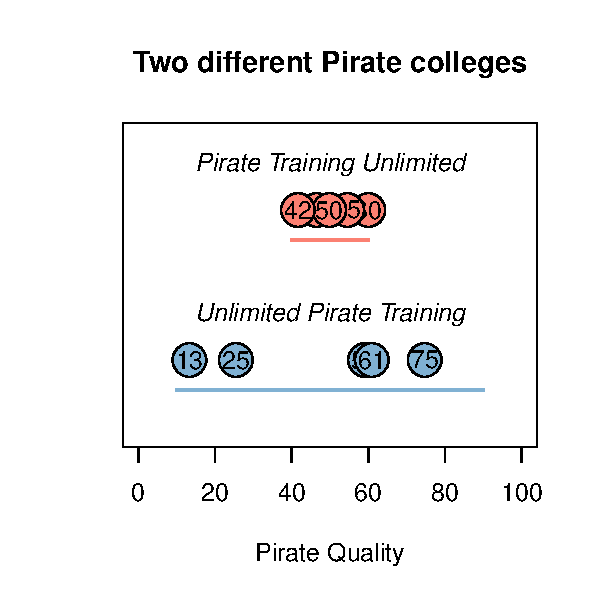
\includegraphics[width=\maxwidth]{figure/unnamed-chunk-155-1} 

\end{knitrout}
\end{tiny}
\caption{Adding text to a plot with text().}
\label{fig:textexample}
\end{marginfigure}

When entering text in the \texttt{labels} argument, keep in mind that R will, by default, plot the entire text in one line. However, if you are adding a long text string (like a sentence), you may want to separate the text into separate lines. To do this, add the text \texttt{"\textbackslash n"} where you want new lines to start. Look at Figure~\ref{fig:manylines} for an example.

\begin{marginfigure} To plot text on separate lines in a plot, put the tag \texttt{"\textbackslash n"} between lines.
\begin{tiny}
\begin{knitrout}
\definecolor{shadecolor}{rgb}{0.969, 0.969, 0.969}\color{fgcolor}\begin{kframe}
\begin{alltt}
\hlkwd{plot}\hlstd{(}\hlnum{1}\hlstd{,} \hlkwc{type} \hlstd{=} \hlstr{"n"}\hlstd{,} \hlkwc{main} \hlstd{=} \hlstr{"The \textbackslash{}\textbackslash{}n tag"}\hlstd{,}
     \hlkwc{xlab} \hlstd{=} \hlstr{""}\hlstd{,} \hlkwc{ylab} \hlstd{=} \hlstr{""}\hlstd{)}

\hlcom{# Text without \textbackslash{}n breaks}
\hlkwd{text}\hlstd{(}\hlkwc{x} \hlstd{=} \hlnum{1}\hlstd{,} \hlkwc{y} \hlstd{=} \hlnum{1.3}\hlstd{,} \hlkwc{labels} \hlstd{=} \hlstr{"Text without \textbackslash{}\textbackslash{}n"}\hlstd{,} \hlkwc{font} \hlstd{=} \hlnum{2}\hlstd{)}
\hlkwd{text}\hlstd{(}\hlkwc{x} \hlstd{=} \hlnum{1}\hlstd{,} \hlkwc{y} \hlstd{=} \hlnum{1.2}\hlstd{,}
     \hlkwc{labels} \hlstd{=} \hlstr{"Haikus are easy. But sometimes they don't make sense. Refrigerator"}
     \hlstd{)}
\hlkwd{abline}\hlstd{(}\hlkwc{h} \hlstd{=} \hlnum{1}\hlstd{,} \hlkwc{lty} \hlstd{=} \hlnum{2}\hlstd{)}
\hlcom{# Text with \textbackslash{}n breaks}
\hlkwd{text}\hlstd{(}\hlkwc{x} \hlstd{=} \hlnum{1}\hlstd{,} \hlkwc{y} \hlstd{=} \hlnum{.92}\hlstd{,} \hlkwc{labels} \hlstd{=} \hlstr{"Text with \textbackslash{}\textbackslash{}n"}\hlstd{,} \hlkwc{font} \hlstd{=} \hlnum{2}\hlstd{)}
\hlkwd{text}\hlstd{(}\hlkwc{x} \hlstd{=} \hlnum{1}\hlstd{,} \hlkwc{y} \hlstd{=} \hlnum{.7}\hlstd{,}
     \hlkwc{labels} \hlstd{=} \hlstr{"Haikus are easy\textbackslash{}nBut sometimes they don't make sense\textbackslash{}nRefrigerator"}
     \hlstd{)}
\end{alltt}
\end{kframe}
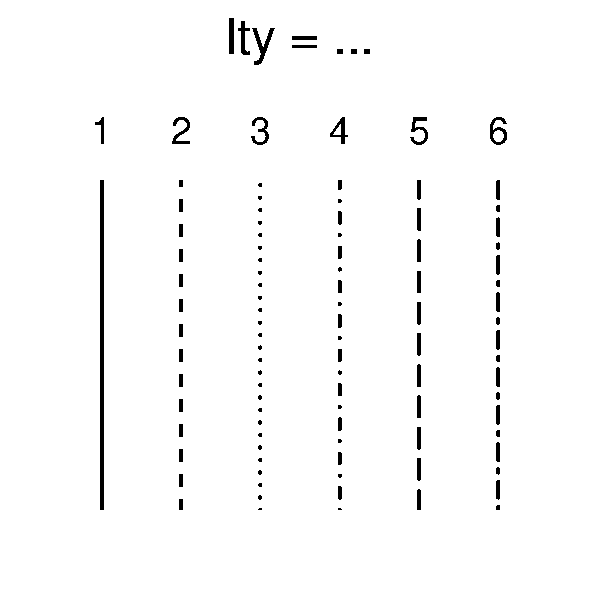
\includegraphics[width=\maxwidth]{figure/unnamed-chunk-156-1} 

\end{knitrout}
\end{tiny}
\label{fig:manylines}
\caption{Using the \texttt{"\textbackslash n"} tag to plot text on separate lines.}
\end{marginfigure}


\subsection{Formatting text for plotting}

A common way to use text in a plot, either in the main title of a plot or using the \texttt{text()} function, is to combine text with numerical data. For example, you may want to include the text "Mean = 3.14" in a plot to show that the mean of the data is 3.14. But how can we combine numerical data with text? In R, we can do this with the \texttt{paste()} function:




\vspace{5mm} %5mm vertical space
\noindent
\setlength{\fboxrule}{1.5pt}
\fbox{
\parbox{\textwidth}{

\newfun{paste()}\index{paste()}

\hline

\begin{description}

\item[\tt{...}] \hfill \\
One or more scalars or vectors (numeric or string) to be combined. For example \texttt{paste("The mean of x is ", mean(x), sep = "")} will create a string combining text and a statistic calculated from data.

\item[\tt{sep}] \hfill \\
A character string that separates the arguments. Set to \texttt{""} for no separation

\end{description}

}
}
\vspace{5mm} %5mm vertical space



The paste function will be helpful to you anytime you want to combine either multiple strings, or text and strings together. For example, let's say you want to write text in a plot that says \texttt{The mean of these data are XXX}, where XXX is replaced by the group mean. To do this, just include the main text and the object referring to the numerical mean as arguments to \texttt{paste()}:\marginnote{When you include descriptive statistics in a plot, you will almost always want to use the \texttt{round(x, digits)} function to reduce the number of digits in the statistic.}

\begin{footnotesize}
\begin{knitrout}
\definecolor{shadecolor}{rgb}{0.969, 0.969, 0.969}\color{fgcolor}\begin{kframe}
\begin{alltt}
\hlstd{data} \hlkwb{<-} \hlkwd{rnorm}\hlstd{(}\hlnum{200}\hlstd{,} \hlkwc{mean} \hlstd{=} \hlnum{20}\hlstd{,} \hlkwc{sd} \hlstd{=} \hlnum{10}\hlstd{)}
\hlkwd{mean}\hlstd{(data)}
\end{alltt}
\begin{verbatim}
## [1] 20.56928
\end{verbatim}
\begin{alltt}
\hlkwd{paste}\hlstd{(}\hlstr{"The mean of the group is"}\hlstd{,} \hlkwd{mean}\hlstd{(data))} \hlcom{# No rounding}
\end{alltt}
\begin{verbatim}
## [1] "The mean of the group is 20.5692797809263"
\end{verbatim}
\begin{alltt}
\hlkwd{paste}\hlstd{(}\hlstr{"The mean of the group is"}\hlstd{,} \hlkwd{round}\hlstd{(}\hlkwd{mean}\hlstd{(data),} \hlnum{2}\hlstd{))} \hlcom{# No rounding}
\end{alltt}
\begin{verbatim}
## [1] "The mean of the group is 20.57"
\end{verbatim}
\end{kframe}
\end{knitrout}
\end{footnotesize}

\end{marginnote}

You can also use vectors as arguments to the \texttt{paste()} function. For example, let's say that you want to create a vector of labels for 5 groups, and you want each group to be labelled \texttt{"Group X"}. We can easily do this with \texttt{paste()}

\begin{footnotesize}
\begin{knitrout}
\definecolor{shadecolor}{rgb}{0.969, 0.969, 0.969}\color{fgcolor}\begin{kframe}
\begin{alltt}
\hlkwd{paste}\hlstd{(}\hlstr{"Group"}\hlstd{,} \hlnum{1}\hlopt{:}\hlnum{5}\hlstd{,} \hlkwc{sep} \hlstd{=} \hlstr{" "}\hlstd{)}
\end{alltt}
\begin{verbatim}
## [1] "Group 1" "Group 2" "Group 3" "Group 4" "Group 5"
\end{verbatim}
\end{kframe}
\end{knitrout}
\end{footnotesize}


\subsection{curve()}

\begin{marginfigure}
\begin{tiny}
\begin{knitrout}
\definecolor{shadecolor}{rgb}{0.969, 0.969, 0.969}\color{fgcolor}\begin{kframe}
\begin{alltt}
\hlkwd{plot}\hlstd{(}\hlnum{1}\hlstd{,} \hlkwc{xlim} \hlstd{=} \hlkwd{c}\hlstd{(}\hlopt{-}\hlnum{5}\hlstd{,} \hlnum{5}\hlstd{),} \hlkwc{ylim} \hlstd{=} \hlkwd{c}\hlstd{(}\hlopt{-}\hlnum{5}\hlstd{,} \hlnum{5}\hlstd{),}
     \hlkwc{type} \hlstd{=} \hlstr{"n"}\hlstd{,} \hlkwc{main} \hlstd{=} \hlstr{"Plotting function lines with curve()"}\hlstd{,}
     \hlkwc{ylab} \hlstd{=} \hlstr{""}\hlstd{,} \hlkwc{xlab} \hlstd{=} \hlstr{""}\hlstd{)}
\hlkwd{abline}\hlstd{(}\hlkwc{h} \hlstd{=} \hlnum{0}\hlstd{)}
\hlkwd{abline}\hlstd{(}\hlkwc{v} \hlstd{=} \hlnum{0}\hlstd{)}

\hlkwd{require}\hlstd{(}\hlstr{"RColorBrewer"}\hlstd{)}
\hlstd{col.vec} \hlkwb{<-} \hlkwd{brewer.pal}\hlstd{(}\hlnum{12}\hlstd{,} \hlkwc{name} \hlstd{=} \hlstr{"Set3"}\hlstd{)[}\hlnum{4}\hlopt{:}\hlnum{7}\hlstd{]}

\hlkwd{curve}\hlstd{(}\hlkwc{expr} \hlstd{= x}\hlopt{^}\hlnum{2}\hlstd{,} \hlkwc{from} \hlstd{=} \hlopt{-}\hlnum{5}\hlstd{,} \hlkwc{to} \hlstd{=} \hlnum{5}\hlstd{,}
      \hlkwc{add} \hlstd{= T,} \hlkwc{lwd} \hlstd{=} \hlnum{2}\hlstd{,} \hlkwc{col} \hlstd{= col.vec[}\hlnum{1}\hlstd{])}
\hlkwd{curve}\hlstd{(}\hlkwc{expr} \hlstd{= x}\hlopt{^}\hlnum{.5}\hlstd{,} \hlkwc{from} \hlstd{=} \hlnum{0}\hlstd{,} \hlkwc{to} \hlstd{=} \hlnum{5}\hlstd{,}
      \hlkwc{add} \hlstd{= T,} \hlkwc{lwd} \hlstd{=} \hlnum{2}\hlstd{,} \hlkwc{col} \hlstd{= col.vec[}\hlnum{2}\hlstd{])}
\hlkwd{curve}\hlstd{(}\hlkwc{expr} \hlstd{= sin,} \hlkwc{from} \hlstd{=} \hlopt{-}\hlnum{5}\hlstd{,} \hlkwc{to} \hlstd{=} \hlnum{5}\hlstd{,}
      \hlkwc{add} \hlstd{= T,} \hlkwc{lwd} \hlstd{=} \hlnum{2}\hlstd{,} \hlkwc{col} \hlstd{= col.vec[}\hlnum{3}\hlstd{])}

\hlstd{my.fun} \hlkwb{<-} \hlkwa{function}\hlstd{(}\hlkwc{x}\hlstd{) \{}\hlkwd{return}\hlstd{(}\hlkwd{dnorm}\hlstd{(x,} \hlkwc{mean} \hlstd{=} \hlnum{2}\hlstd{,} \hlkwc{sd} \hlstd{=} \hlnum{.2}\hlstd{))\}}
\hlkwd{curve}\hlstd{(}\hlkwc{expr} \hlstd{= my.fun,} \hlkwc{from} \hlstd{=} \hlopt{-}\hlnum{5}\hlstd{,} \hlkwc{to} \hlstd{=} \hlnum{5}\hlstd{,}
      \hlkwc{add} \hlstd{= T,} \hlkwc{lwd} \hlstd{=} \hlnum{2}\hlstd{,} \hlkwc{col} \hlstd{= col.vec[}\hlnum{4}\hlstd{])}

\hlkwd{legend}\hlstd{(}\hlstr{"bottomright"}\hlstd{,}
       \hlkwc{legend} \hlstd{=} \hlkwd{c}\hlstd{(}\hlstr{"x^2"}\hlstd{,} \hlstr{"x^.5"}\hlstd{,} \hlstr{"sin(x)"}\hlstd{,} \hlstr{"dnorm(x, 2, .2"}\hlstd{),}
       \hlkwc{col} \hlstd{= col.vec[}\hlnum{1}\hlopt{:}\hlnum{4}\hlstd{],} \hlkwc{lwd} \hlstd{=} \hlnum{2}\hlstd{,}
       \hlkwc{lty} \hlstd{=} \hlnum{1}\hlstd{,} \hlkwc{cex} \hlstd{=} \hlnum{.8}\hlstd{,} \hlkwc{bty} \hlstd{=} \hlstr{"n"}
       \hlstd{)}
\end{alltt}
\end{kframe}
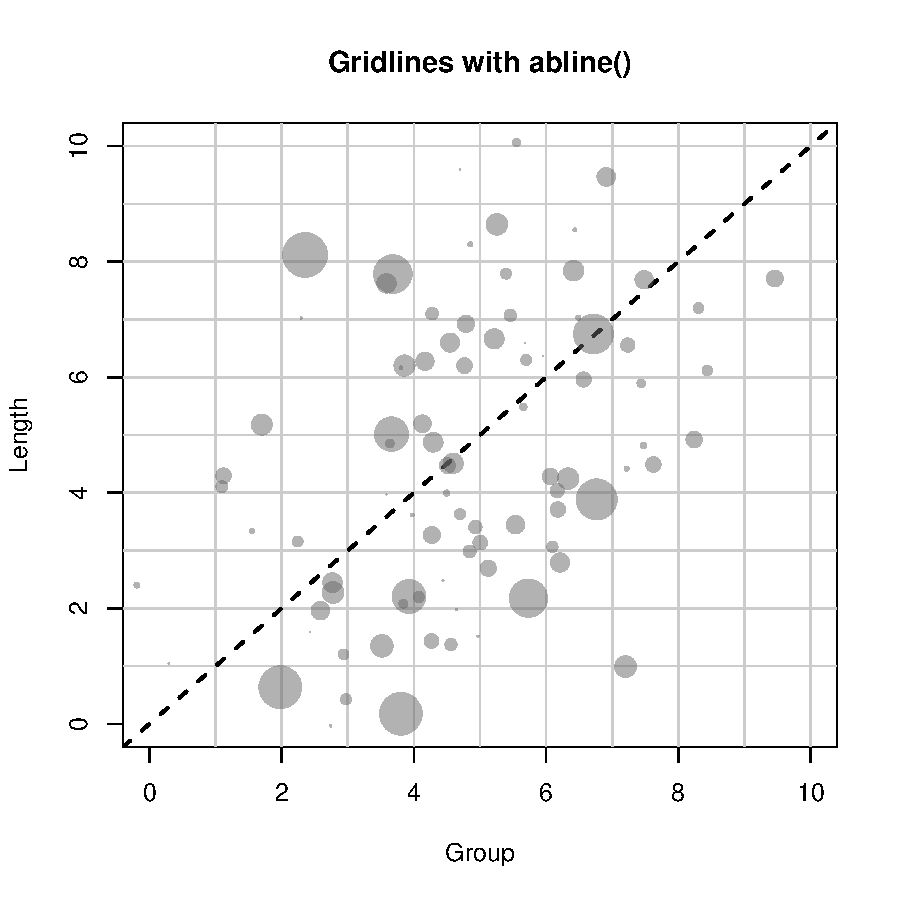
\includegraphics[width=\maxwidth]{figure/unnamed-chunk-159-1} 

\end{knitrout}
\end{tiny}
\caption{Using \texttt{curve()} to easily create lines of functions}
\label{fig:functionlines}
\end{marginfigure}


The \texttt{curve()} function allows you to add a line showing a specific function or equation to a plot


\vspace{5mm} %5mm vertical space
\noindent
\setlength{\fboxrule}{1.5pt}
\fbox{
\parbox{\textwidth}{

\newfun{curve()}\index{curve()}

\hline

\begin{description}

\item[\tt{expr}] \hfill \\
 The name of a function written as a function of \texttt{x} that returns a single vector. You can either use base functions in R like \texttt{expr = $x^2$}, \texttt{expr = x + 4 - 2}, or use your own custom functions such as \texttt{expr = my.fun}, where \texttt{my.fun} is previously defined (e.g.; \texttt{my.fun <- function(x) {dnorm(x, mean = 10, sd = 3)}})

\item[\tt{from, to}] \hfill \\
 The starting (\texttt{from}) and ending (\texttt{to}) value of x to be plotted.

\item[\tt{add}] \hfill \\
 A logical value indicating whether or not to add the curve to an existing plot. If \texttt{add = FALSE}, then \texttt{curve()} will act like a high-level plotting function and create a new plot. If \texttt{add = TRUE}, then \texttt{curve()} will act like a low-level plotting function.

\item[\tt{lty, lwd, col}] \hfill \\
Additional arguments such as \texttt{lty}, \texttt{col}, \texttt{lwd}, ...

\end{description}

}
}
\vspace{5mm} %5mm vertical space

For example, to add the function $x^2$ to a plot from the x-values -10 to 10, you can run the code:

\begin{knitrout}
\definecolor{shadecolor}{rgb}{0.969, 0.969, 0.969}\color{fgcolor}\begin{kframe}
\begin{alltt}
\hlkwd{curve}\hlstd{(}\hlkwc{expr} \hlstd{= x}\hlopt{^}\hlnum{2}\hlstd{,} \hlkwc{from} \hlstd{=} \hlopt{-}\hlnum{10}\hlstd{,} \hlkwc{to} \hlstd{=} \hlnum{10}\hlstd{)}
\end{alltt}
\end{kframe}
\end{knitrout}

If you want to add a custom function to a plot, you can define the function and then use that function name as the argument to \texttt{expr}. For example, to plot the normal distribution with a mean of 10 and standard deviation of 3, you can use this code:

\begin{knitrout}
\definecolor{shadecolor}{rgb}{0.969, 0.969, 0.969}\color{fgcolor}\begin{kframe}
\begin{alltt}
my.fun <- \hlkwd{function}(x) \{\hlkwd{dnorm}(x, mean = 10, sd = 3)\}
\hlkwd{curve}(expr = my.fun, from = -10, to 10)
\end{alltt}
\end{kframe}
\end{knitrout}


In Figure~\ref{fig:functionlines}, I use the \texttt{curve()} function to create curves of several mathematical formulas.


\subsection{legend()}


\begin{marginfigure}
\begin{tiny}
\begin{knitrout}
\definecolor{shadecolor}{rgb}{0.969, 0.969, 0.969}\color{fgcolor}\begin{kframe}
\begin{alltt}
\hlcom{# Generate some random data}
\hlstd{female.x} \hlkwb{<-} \hlkwd{rnorm}\hlstd{(}\hlnum{100}\hlstd{)}
\hlstd{female.y} \hlkwb{<-} \hlstd{female.x} \hlopt{+} \hlkwd{rnorm}\hlstd{(}\hlnum{100}\hlstd{)}
\hlstd{male.x} \hlkwb{<-} \hlkwd{rnorm}\hlstd{(}\hlnum{100}\hlstd{)}
\hlstd{male.y} \hlkwb{<-} \hlstd{male.x} \hlopt{+} \hlkwd{rnorm}\hlstd{(}\hlnum{100}\hlstd{)}

\hlcom{# Create plot with data from females}
\hlkwd{plot}\hlstd{(female.x, female.y,} \hlkwc{pch} \hlstd{=} \hlnum{16}\hlstd{,} \hlkwc{col} \hlstd{=} \hlstr{'blue'}\hlstd{,}
     \hlkwc{xlab} \hlstd{=} \hlstr{"x"}\hlstd{,} \hlkwc{ylab} \hlstd{=} \hlstr{"y"}\hlstd{,} \hlkwc{main} \hlstd{=} \hlstr{"Adding a legend with legend()"}
     \hlstd{)}

\hlcom{# Add data from males}
\hlkwd{points}\hlstd{(male.x, male.y,} \hlkwc{pch} \hlstd{=} \hlnum{16}\hlstd{,} \hlkwc{col} \hlstd{=} \hlstr{'orange'}\hlstd{)}

\hlcom{# Add legend}
\hlkwd{legend}\hlstd{(}\hlstr{"bottomright"}\hlstd{,}
       \hlkwc{legend} \hlstd{=} \hlkwd{c}\hlstd{(}\hlstr{"Females"}\hlstd{,} \hlstr{"Males"}\hlstd{),}
       \hlkwc{col} \hlstd{=} \hlkwd{c}\hlstd{(}\hlstr{'blue'}\hlstd{,} \hlstr{'orange'}\hlstd{),}
       \hlkwc{pch} \hlstd{=} \hlkwd{c}\hlstd{(}\hlnum{16}\hlstd{,} \hlnum{16}\hlstd{),}
       \hlkwc{bg} \hlstd{=} \hlstr{"white"}
       \hlstd{)}
\end{alltt}
\end{kframe}
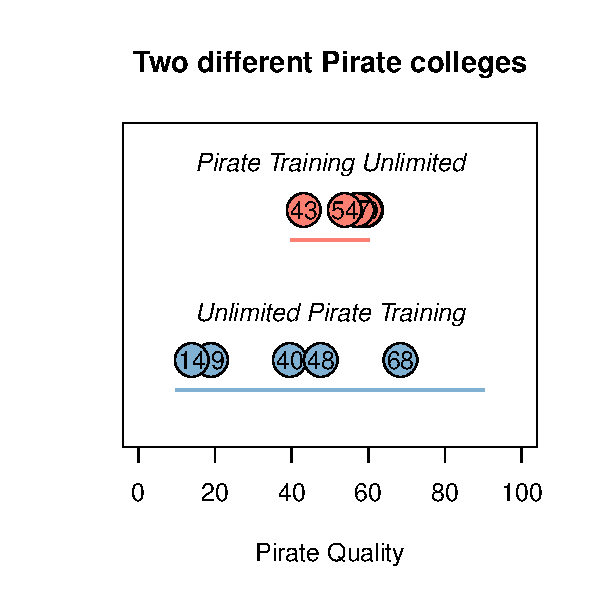
\includegraphics[width=\maxwidth]{figure/unnamed-chunk-162-1} 

\end{knitrout}
\end{tiny}
\label{fig:legendexample}
\caption{Creating a legend labeling the symbol types from different groups}
\end{marginfigure}

The last low-level plotting function that we'll go over in detail is \texttt{legend()} which adds a legend to a plot. This function has the following arguments


\vspace{5mm} %5mm vertical space
\noindent
\setlength{\fboxrule}{1.5pt}
\fbox{
\parbox{\textwidth}{

\newfun{legend()}\index{legend()}

\hline

\begin{description}

\item[\tt{x, y}] \hfill \\
Coordinates of the legend - for example, \texttt{x = 0, y = 0} will put the text at the coordinates (0, 0). Alternatively, you can enter a string indicating where to put the legend (i.e.; "topright", "topleft"). For example, \texttt{"bottomright"} will always put the legend at the bottom right corner of the plot.

\item[\tt{labels}] \hfill \\
  A string vector specifying the text in the legend. For example, \texttt{legend = c("Males, "Females")} will create two groups with names Males and Females.
  
\item[\tt{pch, lty, lwd, col, pt.bg, ...}] \hfill \\
Additional arguments specifying symbol types (\texttt{pch}), line types (\texttt{lty}), line widths (\texttt{lwd}), background color of symbol types 21 thorugh 25 ((\texttt{pt.bg})) and several other optional arguments. See \texttt{?legend} for a complete list


\end{description}

}
}
\vspace{5mm} %5mm vertical space


For example, to add a legend to to bottom-right of an existing graph where data from females are plotted in blue circles and data from males are plotted in pink circles, you'd use the following code:

\begin{knitrout}
\definecolor{shadecolor}{rgb}{0.969, 0.969, 0.969}\color{fgcolor}\begin{kframe}
\begin{alltt}
\hlkwd{legend}\hlstd{(}\hlstr{"bottomright"}\hlstd{,} \hlcom{# Put legend in bottom right of graph}
       \hlkwc{legend} \hlstd{=} \hlkwd{c}\hlstd{(}\hlstr{"Females"}\hlstd{,} \hlstr{"Males"}\hlstd{),} \hlcom{# Names of groups}
       \hlkwc{col} \hlstd{=} \hlkwd{c}\hlstd{(}\hlstr{"blue"}\hlstd{,} \hlstr{"orange"}\hlstd{),} \hlcom{# Colors of symbols}
       \hlkwc{pch} \hlstd{=} \hlkwd{c}\hlstd{(}\hlnum{16}\hlstd{,} \hlnum{16}\hlstd{)} \hlcom{# Point types}
       \hlstd{)}
\end{alltt}
\end{kframe}
\end{knitrout}

In margin Figure~\ref{fig:legendexample} I use this code to add a legend to plot containing data from males and females.



\section{Additional low-level plotting functions}

There are many more low-level plotting functions that can add additional elements to your plots. Here are some I use. To see examples of how to use each one, check out their associated help menus.



\begin{marginfigure}
\begin{tiny}
\begin{knitrout}
\definecolor{shadecolor}{rgb}{0.969, 0.969, 0.969}\color{fgcolor}\begin{kframe}
\begin{alltt}
\hlkwd{par}\hlstd{(}\hlkwc{mar} \hlstd{=} \hlkwd{c}\hlstd{(}\hlnum{0}\hlstd{,} \hlnum{0}\hlstd{,} \hlnum{3}\hlstd{,} \hlnum{0}\hlstd{))}

\hlkwd{plot}\hlstd{(}\hlnum{1}\hlstd{,} \hlkwc{xlim} \hlstd{=} \hlkwd{c}\hlstd{(}\hlnum{1}\hlstd{,} \hlnum{100}\hlstd{),} \hlkwc{ylim} \hlstd{=} \hlkwd{c}\hlstd{(}\hlnum{1}\hlstd{,} \hlnum{100}\hlstd{),}
     \hlkwc{type} \hlstd{=} \hlstr{"n"}\hlstd{,} \hlkwc{xaxt} \hlstd{=} \hlstr{"n"}\hlstd{,} \hlkwc{yaxt} \hlstd{=} \hlstr{"n"}\hlstd{,}
     \hlkwc{ylab} \hlstd{=} \hlstr{""}\hlstd{,} \hlkwc{xlab} \hlstd{=} \hlstr{""}\hlstd{,} \hlkwc{main} \hlstd{=} \hlstr{"Adding simple figures to a plot"}\hlstd{)}

\hlkwd{text}\hlstd{(}\hlnum{25}\hlstd{,} \hlnum{95}\hlstd{,} \hlkwc{labels} \hlstd{=} \hlstr{"rect()"}\hlstd{)}

\hlkwd{rect}\hlstd{(}\hlkwc{xleft} \hlstd{=} \hlnum{10}\hlstd{,} \hlkwc{ybottom} \hlstd{=} \hlnum{70}\hlstd{,}
     \hlkwc{xright} \hlstd{=} \hlnum{40}\hlstd{,} \hlkwc{ytop} \hlstd{=} \hlnum{90}\hlstd{,} \hlkwc{lwd} \hlstd{=} \hlnum{2}\hlstd{,} \hlkwc{col} \hlstd{=} \hlstr{"coral"}\hlstd{)}

\hlkwd{text}\hlstd{(}\hlnum{25}\hlstd{,} \hlnum{60}\hlstd{,} \hlkwc{labels} \hlstd{=} \hlstr{"polygon()"}\hlstd{)}

\hlkwd{polygon}\hlstd{(}\hlkwc{x} \hlstd{=} \hlkwd{runif}\hlstd{(}\hlnum{6}\hlstd{,} \hlnum{15}\hlstd{,} \hlnum{35}\hlstd{),}
        \hlkwc{y} \hlstd{=} \hlkwd{runif}\hlstd{(}\hlnum{6}\hlstd{,} \hlnum{40}\hlstd{,} \hlnum{55}\hlstd{),}
        \hlkwc{col} \hlstd{=} \hlstr{"skyblue"}
        \hlstd{)}


\hlcom{# polygon(x = c(15, 35, 25, 15),}
\hlcom{#         y = c(40, 40, 55, 40),}
\hlcom{#         col = "skyblue"}
\hlcom{#         )}

\hlkwd{text}\hlstd{(}\hlnum{25}\hlstd{,} \hlnum{30}\hlstd{,} \hlkwc{labels} \hlstd{=} \hlstr{"segments()"}\hlstd{)}

\hlkwd{segments}\hlstd{(}\hlkwc{x0} \hlstd{=} \hlkwd{runif}\hlstd{(}\hlnum{5}\hlstd{,} \hlnum{10}\hlstd{,} \hlnum{40}\hlstd{),}
         \hlkwc{y0} \hlstd{=} \hlkwd{runif}\hlstd{(}\hlnum{5}\hlstd{,} \hlnum{5}\hlstd{,} \hlnum{25}\hlstd{),}
         \hlkwc{x1} \hlstd{=} \hlkwd{runif}\hlstd{(}\hlnum{5}\hlstd{,} \hlnum{10}\hlstd{,} \hlnum{40}\hlstd{),}
         \hlkwc{y1} \hlstd{=} \hlkwd{runif}\hlstd{(}\hlnum{5}\hlstd{,} \hlnum{5}\hlstd{,} \hlnum{25}\hlstd{),} \hlkwc{lwd} \hlstd{=} \hlnum{2}
         \hlstd{)}

\hlkwd{text}\hlstd{(}\hlnum{75}\hlstd{,} \hlnum{95}\hlstd{,} \hlkwc{labels} \hlstd{=} \hlstr{"symbols(circles)"}\hlstd{)}

\hlkwd{symbols}\hlstd{(}\hlkwc{x} \hlstd{=} \hlkwd{runif}\hlstd{(}\hlnum{3}\hlstd{,} \hlnum{60}\hlstd{,} \hlnum{90}\hlstd{),}
        \hlkwc{y} \hlstd{=} \hlkwd{runif}\hlstd{(}\hlnum{3}\hlstd{,} \hlnum{60}\hlstd{,} \hlnum{70}\hlstd{),}
        \hlkwc{circles} \hlstd{=} \hlkwd{c}\hlstd{(}\hlnum{1}\hlstd{,} \hlnum{.1}\hlstd{,} \hlnum{.3}\hlstd{),}
        \hlkwc{add} \hlstd{= T,} \hlkwc{bg} \hlstd{=} \hlkwd{gray}\hlstd{(}\hlnum{.5}\hlstd{,} \hlnum{.1}\hlstd{))}

\hlkwd{text}\hlstd{(}\hlnum{75}\hlstd{,} \hlnum{30}\hlstd{,} \hlkwc{labels} \hlstd{=} \hlstr{"arrows()"}\hlstd{)}

\hlkwd{arrows}\hlstd{(}\hlkwc{x0} \hlstd{=} \hlkwd{runif}\hlstd{(}\hlnum{3}\hlstd{,} \hlnum{60}\hlstd{,} \hlnum{90}\hlstd{),}
         \hlkwc{y0} \hlstd{=} \hlkwd{runif}\hlstd{(}\hlnum{3}\hlstd{,} \hlnum{10}\hlstd{,} \hlnum{25}\hlstd{),}
         \hlkwc{x1} \hlstd{=} \hlkwd{runif}\hlstd{(}\hlnum{3}\hlstd{,} \hlnum{60}\hlstd{,} \hlnum{90}\hlstd{),}
         \hlkwc{y1} \hlstd{=} \hlkwd{runif}\hlstd{(}\hlnum{3}\hlstd{,} \hlnum{10}\hlstd{,} \hlnum{25}\hlstd{),}
         \hlkwc{length} \hlstd{=} \hlnum{.1}\hlstd{,} \hlkwc{lwd} \hlstd{=} \hlnum{2}
         \hlstd{)}
\end{alltt}
\end{kframe}
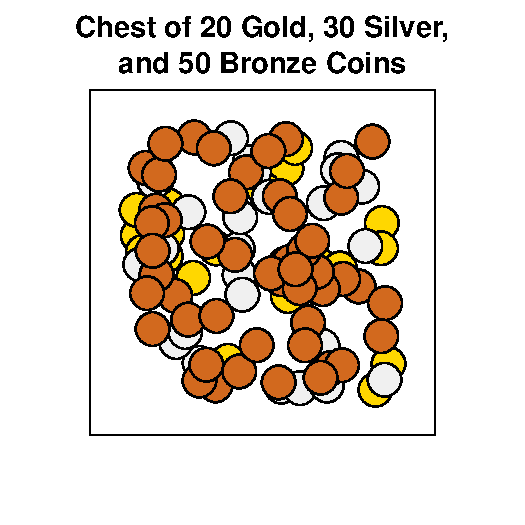
\includegraphics[width=\maxwidth]{figure/unnamed-chunk-164-1} 

\end{knitrout}
\end{tiny}
\end{marginfigure}


\vspace{5mm} %5mm vertical space
\noindent
\setlength{\fboxrule}{1.5pt}
\fbox{
\parbox{\textwidth}{

\newfun{Additional low-level plotting functions}

\hline

\begin{description}

\item[\tt{rect()}] \hfill \\
    Add rectangles to a plot at coordinates specified by \texttt{xleft, ybottom, xright, ybottom}. For example, to add a rectangle with corners at (0, 0) and c(10, 10), specify \texttt{xleft = 0, ybottom = 0, xright = 10, ytop = 10}. Additional arguments like \texttt{col, border} change the color of the rectangle.

\item[\tt{polygon()}] \hfill \\
    Add a polygon to a plot at coordinates specified by vectors x and y. Additional arguments such as \texttt{col, border} change the color of the inside and border of the polygon

\item[\tt{segments(), arrows()}] \hfill \\
 Add segments (lines with fixed endings), or arrows to a plot.
 
\item[\tt{symbols(add = T)}] \hfill \\
Add symbols (circles, squares, rectangles, stars, thermometers) to a plot. The dimensions of each symbol are specified with specific input types. See \texttt{?symbols} for details. Specify \texttt{add = T} to add to an existing plot or \texttt{add = F} to create a new plot.
 
\item[\tt{axis()}] \hfill \\
 Add an additional axis to a plot (or add fully customizable  x and y axes). Usually you only use this if you set \texttt{xaxt = "n", yaxt = "n"} in the original high-level plotting function.
 
\item [\tt{mtext()}] \hfill \\
 Add text to the margins of a plot. Look at the help menu for \texttt{mtext()} to see parameters for this function.
\end{description}

}
}
\vspace{5mm} %5mm vertical space




\section{Saving plots to a file}

Once you've created a plot in R, you may wish to save it to a file so you can use it in another document. To do this, you'll use either the \texttt{pdf()} or \texttt{jpeg()} functions. These functions will save your plot to either a .pdf of jpeg file.


\vspace{5mm} %5mm vertical space
\noindent
\setlength{\fboxrule}{1.5pt}
\fbox{
\parbox{\textwidth}{

\newfun{pdf() and jpeg()}

\hline

\begin{description}

\item[\tt{file}] \hfill \\
    The name and file destination of the final plot entered as a string. For example, to put a plot on my desktop, I'd write \texttt{file = "/Users/Nathaniel/Desktop/plot.pdf"} when creating a pdf, and \texttt{file = "/Users/Nathaniel/Desktop/plot.jpg"} when creating a jpeg.

\item[\tt{width, height}] \hfill \\
    The width and height of the final plot in inches.

\item[\tt{family()}] \hfill \\
An optional name of the font family to use for the plot. For example, \texttt{family = "Helvetica"} will use the Helvetica font for all text (assuming you have Helvetica on your system). For more help on using different fonts, look at section "Using extra fonts in R" in Chapter XX

\item[\tt{dev.off()}] \hfill \\
This is \textit{not} an argument to \texttt{pdf()} and \texttt{jpeg()}. You just need to execute this code after creating the plot to finish creating the image file (see examples below).
 
\end{description}

}
}
\vspace{5mm} %5mm vertical space

To use these functions to save files, you need to follow 3 steps

\begin{enumerate}
  \item Execute the \texttt{pdf()} or \texttt{jpeg()} functions with \texttt{file, width} and \textt{height} arguments.
  \item Execute all your plotting code.
  \item Complete the file by executing the command \texttt{dev.off()}. This tells R that you're done creating the file.
\end{enumerate}

Here's an example of the three steps.


\begin{knitrout}
\definecolor{shadecolor}{rgb}{0.969, 0.969, 0.969}\color{fgcolor}\begin{kframe}
\begin{alltt}
\hlcom{# Step 1: Call the pdf command}
\hlkwd{pdf}\hlstd{(}\hlkwc{file} \hlstd{=} \hlstr{"/Users/Nathaniel/Desktop/My Plot.pdf"}\hlstd{,}   \hlcom{# The directory you want to save the file in}
    \hlkwc{width} \hlstd{=} \hlnum{4}\hlstd{,} \hlcom{# The width of the plot in inches}
    \hlkwc{height} \hlstd{=} \hlnum{4} \hlcom{# The height of the plot in inches}
    \hlstd{)}

\hlcom{# Step 2: Create the plot}
\hlkwd{plot}\hlstd{(}\hlnum{1}\hlopt{:}\hlnum{10}\hlstd{,} \hlnum{1}\hlopt{:}\hlnum{10}\hlstd{)}
\hlkwd{abline}\hlstd{(}\hlkwc{v} \hlstd{=} \hlnum{0}\hlstd{)} \hlcom{# Additional low-level plotting commands}
\hlkwd{text}\hlstd{(}\hlkwc{x} \hlstd{=} \hlnum{0}\hlstd{,} \hlkwc{y} \hlstd{=} \hlnum{1}\hlstd{,} \hlkwc{labels} \hlstd{=} \hlstr{"Random text"}\hlstd{)}

\hlcom{# Step 3: Run dev.off() to create the file!}
\hlkwd{dev.off}\hlstd{()}
\end{alltt}
\end{kframe}
\end{knitrout}


You'll notice that after you close the plot with \texttt{dev.off()}, you'll see a message in the prompt like "null device".

Using the command  \texttt{pdf()} will save the file as a pdf. If you use  \texttt{jpeg()}, it will be saved as a jpeg.


\section{A worked example: Creating a plot with automated numeric labels}


Let's use the \texttt{paste()} command to create a histogram with labels indicating the mean, median, min, and mean of the dataset. We'll do this in 5 steps

1. Generate the data and the histogram\\
2. Add text and reference line for the mean\\
3. Add text and reference line for the minimum\\
4. Add text and reference line for the maximum\\
5. Add a subtitle in full sentences with each summary statistic.

\begin{footnotesize}
\begin{knitrout}
\definecolor{shadecolor}{rgb}{0.969, 0.969, 0.969}\color{fgcolor}\begin{kframe}
\begin{alltt}
\hlcom{# Step 1: Generate data and main histogram}
\hlstd{data} \hlkwb{<-} \hlkwd{rnorm}\hlstd{(}\hlnum{100}\hlstd{,} \hlkwc{mean} \hlstd{=} \hlnum{20}\hlstd{,} \hlkwc{sd} \hlstd{=} \hlnum{2}\hlstd{)}

\hlstd{title.text} \hlkwb{<-} \hlkwd{paste}\hlstd{(}
  \hlstr{"Note: There were "}\hlstd{,} \hlkwd{length}\hlstd{(data),} \hlstr{" data points. The mean and median of the data were "}\hlstd{,}
  \hlkwd{round}\hlstd{(}\hlkwd{mean}\hlstd{(data),} \hlnum{2}\hlstd{),} \hlstr{" and "}\hlstd{,} \hlkwd{round}\hlstd{(}\hlkwd{median}\hlstd{(data,} \hlnum{2}\hlstd{)),} \hlstr{".\textbackslash{}nThe minimum and maximum values were "}\hlstd{,}
  \hlkwd{round}\hlstd{(}\hlkwd{min}\hlstd{(data),} \hlnum{2}\hlstd{),} \hlstr{" and "}\hlstd{,} \hlkwd{round}\hlstd{(}\hlkwd{max}\hlstd{(data),} \hlnum{2}\hlstd{),} \hlstr{"."}\hlstd{,} \hlkwc{sep} \hlstd{=} \hlstr{""}\hlstd{)}


\hlkwd{hist}\hlstd{(data,}
     \hlkwc{xlim} \hlstd{=} \hlkwd{c}\hlstd{(}\hlnum{10}\hlstd{,} \hlnum{30}\hlstd{),}
     \hlkwc{ylim} \hlstd{=} \hlkwd{c}\hlstd{(}\hlnum{0}\hlstd{,} \hlnum{40}\hlstd{),}
     \hlkwc{main} \hlstd{= title.text,}
     \hlkwc{cex.main} \hlstd{=} \hlnum{.7}
     \hlstd{)}

\hlcom{# Step 2: Add mean text and line}
\hlkwd{text}\hlstd{(}\hlkwd{mean}\hlstd{(data),} \hlnum{38}\hlstd{,}
     \hlkwc{labels} \hlstd{=} \hlkwd{paste}\hlstd{(}\hlstr{"Mean\textbackslash{}n"}\hlstd{,} \hlkwd{round}\hlstd{(}\hlkwd{mean}\hlstd{(data),} \hlnum{2}\hlstd{),} \hlkwc{sep} \hlstd{=} \hlstr{""}\hlstd{),}
     \hlkwc{adj} \hlstd{=} \hlnum{0}\hlstd{,}
     \hlkwc{pos} \hlstd{=} \hlnum{4}
\hlstd{)}
\hlkwd{abline}\hlstd{(}\hlkwc{v} \hlstd{=} \hlkwd{mean}\hlstd{(data),} \hlkwc{lty} \hlstd{=} \hlnum{2}\hlstd{)}

\hlcom{# Step 3: Add minimum text and line}
\hlkwd{text}\hlstd{(}\hlkwd{min}\hlstd{(data),} \hlnum{25}\hlstd{,}
     \hlkwc{labels} \hlstd{=} \hlkwd{paste}\hlstd{(}\hlstr{"Min\textbackslash{}n"}\hlstd{,} \hlkwd{round}\hlstd{(}\hlkwd{min}\hlstd{(data),} \hlnum{2}\hlstd{),} \hlkwc{sep} \hlstd{=} \hlstr{""}\hlstd{),}
     \hlkwc{adj} \hlstd{=} \hlnum{0}\hlstd{,}
     \hlkwc{pos} \hlstd{=} \hlnum{2}
\hlstd{)}

\hlkwd{abline}\hlstd{(}\hlkwc{v} \hlstd{=} \hlkwd{min}\hlstd{(data),} \hlkwc{lty} \hlstd{=} \hlnum{2}\hlstd{)}

\hlcom{# Step 4: Add maximum text and line}
\hlkwd{text}\hlstd{(}\hlkwd{max}\hlstd{(data),} \hlnum{25}\hlstd{,}
     \hlkwc{labels} \hlstd{=} \hlkwd{paste}\hlstd{(}\hlstr{"Max\textbackslash{}n"}\hlstd{,} \hlkwd{round}\hlstd{(}\hlkwd{min}\hlstd{(data),} \hlnum{2}\hlstd{),} \hlkwc{sep} \hlstd{=} \hlstr{""}\hlstd{),}
     \hlkwc{adj} \hlstd{=} \hlnum{0}\hlstd{,}
     \hlkwc{pos} \hlstd{=} \hlnum{4}
\hlstd{)}

\hlkwd{abline}\hlstd{(}\hlkwc{v} \hlstd{=} \hlkwd{max}\hlstd{(data),} \hlkwc{lty} \hlstd{=} \hlnum{2}\hlstd{)}
\end{alltt}
\end{kframe}
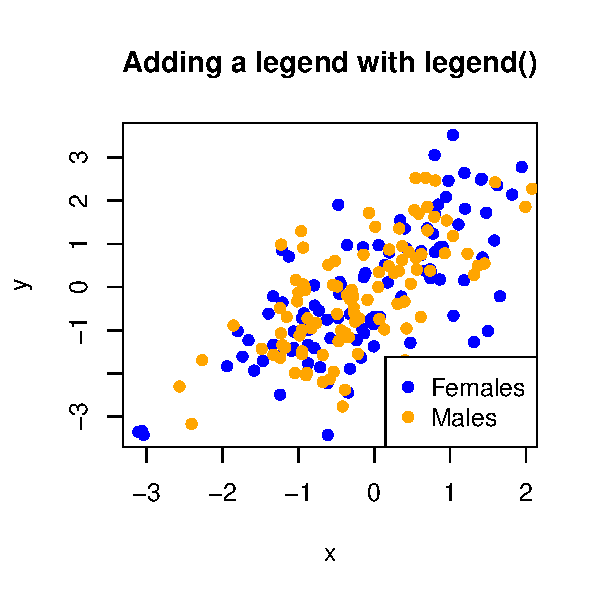
\includegraphics[width=\maxwidth]{figure/unnamed-chunk-166-1} 

\end{knitrout}
\end{footnotesize}

The benefit of using \texttt{paste()} over hard-coding the text (for example by typing \texttt{labels = "Mean = 20"}) is that the code will automatically change the value of the mean when the data changes. To see this in action, run the code above several times and see how the numbers automatically update. In later chapters, when use loops to create multiple graphs over different sets of data, this will become extremely helpful!


\section{Additional Tips}

\begin{itemize}
  
  \item Many high-level plotting functions can be used like low-level plotting functions if you add an additional argument like \texttt{new = F} or \texttt{add = T}. Look at the help menu for specific high-level functions to see which arguments allow you to add a high-level plot to an existing plot.
  

\end{itemize}





%----------------------------------------------------------------------------------------
%	CHAPTER 8
%----------------------------------------------------------------------------------------

\chapter{8: Customizing Plots}
\label{ch:8}

\begin{enumerate}

  \item Specifying and creating colors
  \item Specifying plot margins with \texttt{par(mar)}
  \item Putting several plots together with \texttt{par(mfrow)} and \texttt{layout}
  \item Using different fonts in plots

\end{enumerate}



\section{Colors in R}

There are many ways to specify colors in R. If you want to specify a color directly, you can do that in one of the following ways:

\subsection{Specifying colors as a string}
  
The easiest way to specify a color is to just write its name as a string. For example, you can write \texttt{"blue"}, \texttt{"lightgreen"}, \texttt{"red"}, among many other colors. To see a list of all the named colors, look at the vector \texttt{colors()} which contains all 657 named colors in R. Here is a random sample of 10 of them (to see all the colors, look at the color graph in the Appendix)
  
\begin{footnotesize}
\begin{knitrout}
\definecolor{shadecolor}{rgb}{0.969, 0.969, 0.969}\color{fgcolor}\begin{kframe}
\begin{alltt}
\hlkwd{colors}\hlstd{()[}\hlkwd{sample}\hlstd{(}\hlnum{1}\hlopt{:}\hlkwd{length}\hlstd{(}\hlkwd{colors}\hlstd{()),} \hlnum{10}\hlstd{)]}
\end{alltt}
\begin{verbatim}
##  [1] "coral2"       "gold1"        "grey72"       "darkseagreen"
##  [5] "dodgerblue"   "gray79"       "violetred"    "orange4"     
##  [9] "darkorange2"  "red1"
\end{verbatim}
\end{kframe}
\end{knitrout}
\end{footnotesize}

\subsection{Shades of gray with \texttt{gray()}}
  
If you're a lonely, sexually repressed, 50+ year old housewife, then you might want to stick with shades of gray. If so, the function \texttt{gray(x)} is your answer. \texttt{gray()} is a function that takes a number (or vector of numbers) between 0 and 1 as an argument, and returns a shade of gray (or many shades of gray with a vector input). A value of 1 is equivalent to \texttt{"white"} while 0 is equivalent to \texttt{"black"}. This function is very helpful if you want to create shades of gray depending on the value of a numeric vector. For example, if you had survey data and plotted income on the x-axis and happiness on the y-axis of a scatterplot, you could determine the darkness of each point as a function of a third quantitative variable (such as number of children or amount of travel time to work). I plotted an example of this in Figure~\ref{fig:incomegray}.

\begin{marginfigure}

\begin{tiny}
\begin{knitrout}
\definecolor{shadecolor}{rgb}{0.969, 0.969, 0.969}\color{fgcolor}\begin{kframe}
\begin{alltt}
\hlstd{inc} \hlkwb{<-} \hlkwd{rnorm}\hlstd{(}\hlkwc{n} \hlstd{=} \hlnum{200}\hlstd{,} \hlkwc{mean} \hlstd{=} \hlnum{50}\hlstd{,} \hlkwc{sd} \hlstd{=} \hlnum{10}\hlstd{)}
\hlstd{hap} \hlkwb{<-} \hlstd{inc} \hlopt{+} \hlkwd{rnorm}\hlstd{(}\hlkwc{n} \hlstd{=} \hlnum{200}\hlstd{,} \hlkwc{mean} \hlstd{=} \hlnum{0}\hlstd{,} \hlkwc{sd} \hlstd{=} \hlnum{15}\hlstd{)}
\hlstd{drive} \hlkwb{<-} \hlstd{inc} \hlopt{+} \hlkwd{rnorm}\hlstd{(}\hlkwc{n} \hlstd{=} \hlnum{200}\hlstd{,} \hlkwc{mean} \hlstd{=} \hlnum{0}\hlstd{,} \hlkwc{sd} \hlstd{=} \hlnum{5}\hlstd{)}

\hlkwd{plot}\hlstd{(}\hlkwc{x} \hlstd{= inc,} \hlkwc{y} \hlstd{= hap,} \hlkwc{pch} \hlstd{=} \hlnum{16}\hlstd{,}
     \hlkwc{col} \hlstd{=} \hlkwd{gray}\hlstd{((drive} \hlopt{-} \hlkwd{min}\hlstd{(drive))} \hlopt{/} \hlkwd{max}\hlstd{(drive} \hlopt{-} \hlkwd{min}\hlstd{(drive)),} \hlkwc{alpha} \hlstd{=} \hlnum{.4}\hlstd{),}
     \hlkwc{cex} \hlstd{=} \hlnum{1.5}\hlstd{,}
     \hlkwc{xlab} \hlstd{=} \hlstr{"income"}\hlstd{,} \hlkwc{ylab} \hlstd{=} \hlstr{"happiness"}
     \hlstd{)}
\end{alltt}
\end{kframe}
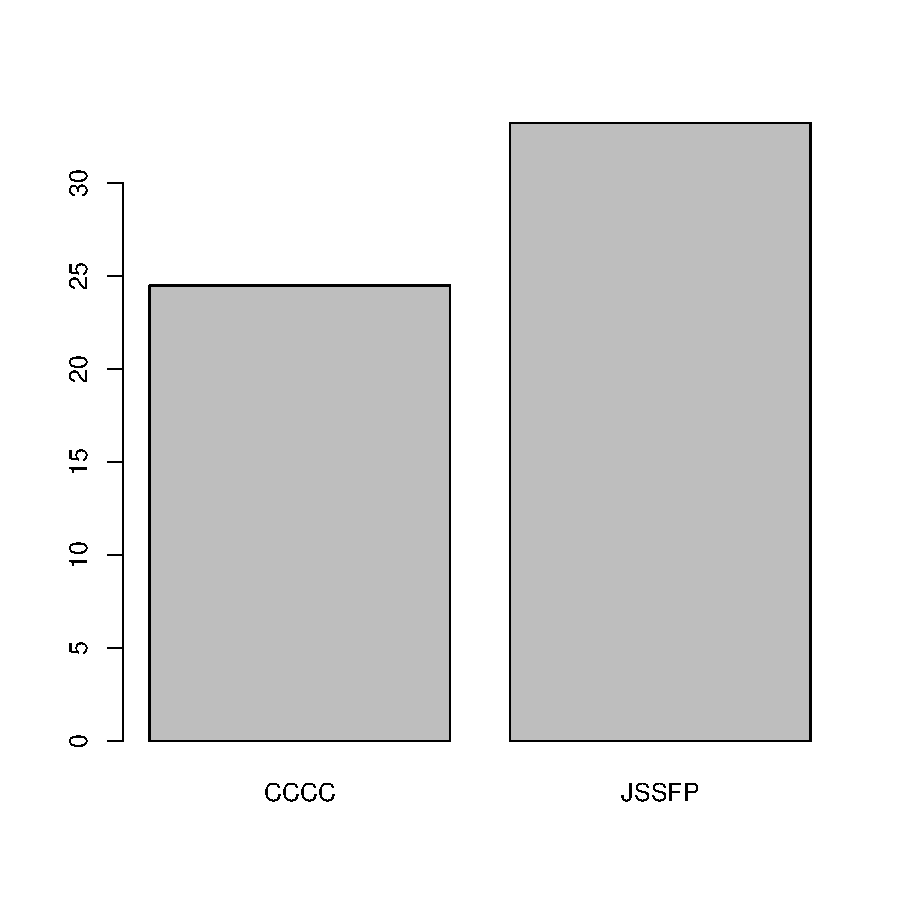
\includegraphics[width=\maxwidth]{figure/unnamed-chunk-168-1} 

\end{knitrout}
\end{tiny}
\caption{Using the \texttt{gray()} function to easily create shades of gray in plotting symbols based on numerical data.}
\label{fig:incomegray}
\end{marginfigure}

\subsection{RGB values: \texttt{rgb()}}

Every color can be defined by its RGB ("Red", "Green", "Blue") value. This value specifies the combination of shades of Red, Green and Blue that create that color. Traditionally, each color shade is defined on a scale from 0 to 255. For example, the RGB value [255, 0, 0] is pure Red, while [0, 255, 0] is pure Green.

To create a color from RGB values, use the function \texttt{rgb()}


\vspace{5mm} %5mm vertical space
\noindent
\setlength{\fboxrule}{1.5pt}
\fbox{
\parbox{\textwidth}{

\newfun{rgb()}\index{rgb()}

\hline

\begin{description}

\item[\tt{red, green blue}] \hfill \\
Numeric arguments indicating the strength of red, green, and blue heus

\item[\tt{maxColorValue}] \hfill \\
A number indicating the maximum possible hue value. The default is 1 - however, most people use \texttt{maxColorValue = 255}
  
\item[\tt{alpha}] \hfill \\
The opacity of the color(s) inputted as a number between 0 and \texttt{maxColorValue}


\end{description}

}
}
\vspace{5mm} %5mm vertical space



When you use the function \texttt{rgb()}, the function will return a string as output. The string will look like nonsense to you, but that's just how R names colors:

\begin{footnotesize}
\begin{knitrout}
\definecolor{shadecolor}{rgb}{0.969, 0.969, 0.969}\color{fgcolor}\begin{kframe}
\begin{alltt}
\hlkwd{rgb}\hlstd{(}\hlkwc{red} \hlstd{=} \hlnum{0}\hlstd{,} \hlkwc{green} \hlstd{=} \hlnum{255}\hlstd{,} \hlkwc{blue} \hlstd{=} \hlnum{0}\hlstd{,} \hlkwc{maxColorValue} \hlstd{=} \hlnum{255}\hlstd{)} \hlcom{# pure red}
\end{alltt}
\begin{verbatim}
## [1] "#00FF00"
\end{verbatim}
\begin{alltt}
\hlkwd{rgb}\hlstd{(}\hlkwc{red} \hlstd{=} \hlnum{0}\hlstd{,} \hlkwc{green} \hlstd{=} \hlnum{255}\hlstd{,} \hlkwc{blue} \hlstd{=} \hlnum{0}\hlstd{,} \hlkwc{alpha} \hlstd{=} \hlnum{100}\hlstd{,} \hlkwc{maxColorValue} \hlstd{=} \hlnum{255}\hlstd{)} \hlcom{# transparent red}
\end{alltt}
\begin{verbatim}
## [1] "#00FF0064"
\end{verbatim}
\begin{alltt}
\hlkwd{rgb}\hlstd{(}\hlkwc{red} \hlstd{=} \hlnum{100}\hlstd{,} \hlkwc{green} \hlstd{=} \hlnum{100}\hlstd{,} \hlkwc{blue} \hlstd{=} \hlnum{100}\hlstd{,} \hlkwc{maxColorValue} \hlstd{=} \hlnum{255}\hlstd{)} \hlcom{# even mixture}
\end{alltt}
\begin{verbatim}
## [1] "#646464"
\end{verbatim}
\end{kframe}
\end{knitrout}
\end{footnotesize}

Now, if you're not used to interpreting colors as RGB values, you may gloss over this section and think you'll never use it. However, look at this chapter's \textit{Additional Tips} for a really cool method of 'stealing' the exact color from \textit{anything} on your computer screen and using \texttt{rgb()} to then use that color in your R plots!

\subsection{Color Palettes with the \texttt{RColorBrewer} package}

If you use many colors in the same plot, it's probably a good idea to choose colors that compliment each other. An easy way to select colors that go well together is to use a \textit{color palette} - a collection of colors known to go well together.

One package that is great for getting (and even creating) palettes is \texttt{RColorBrewer}. Here are some of the palettes in the package. The name of each palette is in the first column, and the colors in each palette are in each row:


\begin{knitrout}
\definecolor{shadecolor}{rgb}{0.969, 0.969, 0.969}\color{fgcolor}\begin{kframe}
\begin{alltt}
\hlkwd{require}\hlstd{(}\hlstr{"RColorBrewer"}\hlstd{)}
\hlkwd{display.brewer.all}\hlstd{()}
\end{alltt}
\end{kframe}
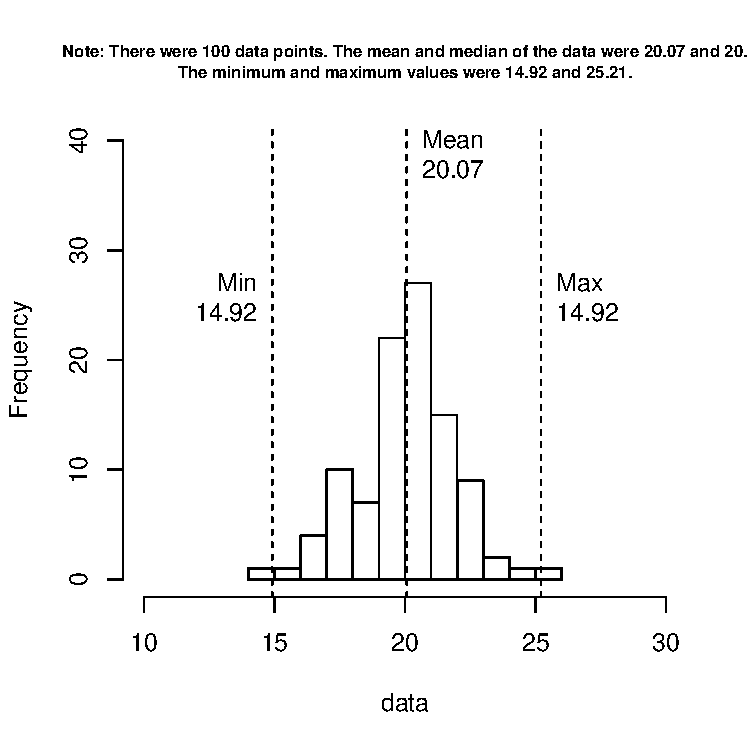
\includegraphics[width=\maxwidth]{figure/unnamed-chunk-170-1} 

\end{knitrout}


To use one of the palettes, execute the function \texttt{brewer.pal(n, name)}, where \texttt{n} is the number of colors you want, and \texttt{name} is the name of the palette. For example, to get 4 colors from the color set ``Set1", you'd use the code

\begin{footnotesize}
\begin{knitrout}
\definecolor{shadecolor}{rgb}{0.969, 0.969, 0.969}\color{fgcolor}\begin{kframe}
\begin{alltt}
\hlstd{my.colors} \hlkwb{<-} \hlkwd{brewer.pal}\hlstd{(}\hlnum{4}\hlstd{,} \hlstr{"Set1"}\hlstd{)} \hlcom{# 4 colors from Set1}
\hlstd{my.colors}
\end{alltt}
\begin{verbatim}
## [1] "#E41A1C" "#377EB8" "#4DAF4A" "#984EA3"
\end{verbatim}
\end{kframe}
\end{knitrout}
\end{footnotesize}

I know the results look like gibberish, but trust me, R will interpret them as the colors in the palette. Once you store the output of the \texttt{brewer.pal()} function as a vector (something like \texttt{my.colors}), you can then use this vector as an argument for the colors in your plot.

\subsection{Numerically defined color gradients with \texttt{colorRamp2}}

My favorite way to generate colors that represent numerical data is with the function \texttt{colorRamp2} in the \texttt{circlize} package (the same package that creates that really cool \texttt{chordDiagram} from Chapter 1). The \texttt{colorRamp2} function allows you to easily generate shades of colors based on numerical data. 

\begin{marginfigure}
\begin{tiny}
\begin{knitrout}
\definecolor{shadecolor}{rgb}{0.969, 0.969, 0.969}\color{fgcolor}\begin{kframe}
\begin{alltt}
\hlkwd{require}\hlstd{(}\hlstr{"RColorBrewer"}\hlstd{)}
\hlkwd{require}\hlstd{(}\hlstr{"circlize"}\hlstd{)}

\hlcom{# Create Data}
\hlstd{drinks} \hlkwb{<-} \hlkwd{sample}\hlstd{(}\hlnum{1}\hlopt{:}\hlnum{30}\hlstd{,} \hlkwc{size} \hlstd{=} \hlnum{100}\hlstd{,} \hlkwc{replace} \hlstd{= T)}
\hlstd{smokes} \hlkwb{<-} \hlkwd{sample}\hlstd{(}\hlnum{1}\hlopt{:}\hlnum{30}\hlstd{,} \hlkwc{size} \hlstd{=} \hlnum{100}\hlstd{,} \hlkwc{replace} \hlstd{= T)}
\hlstd{risk} \hlkwb{<-} \hlnum{1} \hlopt{/} \hlstd{(}\hlnum{1} \hlopt{+} \hlkwd{exp}\hlstd{(}\hlopt{-}\hlstd{drinks} \hlopt{/} \hlnum{20} \hlopt{+} \hlkwd{rnorm}\hlstd{(}\hlnum{100}\hlstd{,} \hlkwc{mean} \hlstd{=} \hlnum{0}\hlstd{,} \hlkwc{sd} \hlstd{=} \hlnum{1}\hlstd{)))}

\hlcom{# Create color function from colorRamp2}
\hlstd{smoking.colors} \hlkwb{<-} \hlkwd{colorRamp2}\hlstd{(}\hlkwc{breaks} \hlstd{=} \hlkwd{c}\hlstd{(}\hlnum{0}\hlstd{,} \hlnum{15}\hlstd{,} \hlnum{30}\hlstd{),}
                  \hlkwc{colors} \hlstd{=} \hlkwd{c}\hlstd{(}\hlstr{"blue"}\hlstd{,} \hlstr{"orange"}\hlstd{,} \hlstr{"red"}\hlstd{),}
                  \hlkwc{transparency} \hlstd{=} \hlnum{.3}
                  \hlstd{)}

\hlcom{# Set up plot layout}
\hlkwd{layout}\hlstd{(}\hlkwc{mat} \hlstd{=} \hlkwd{matrix}\hlstd{(}\hlkwd{c}\hlstd{(}\hlnum{1}\hlstd{,} \hlnum{2}\hlstd{),} \hlkwc{nrow} \hlstd{=} \hlnum{2}\hlstd{,} \hlkwc{ncol} \hlstd{=} \hlnum{1}\hlstd{),}
       \hlkwc{heights} \hlstd{=} \hlkwd{c}\hlstd{(}\hlnum{2.5}\hlstd{,} \hlnum{5}\hlstd{),} \hlkwc{widths} \hlstd{=} \hlnum{4}\hlstd{)}

\hlcom{# Top Plot}
\hlkwd{par}\hlstd{(}\hlkwc{mar} \hlstd{=} \hlkwd{c}\hlstd{(}\hlnum{4}\hlstd{,} \hlnum{4}\hlstd{,} \hlnum{2}\hlstd{,} \hlnum{1}\hlstd{))}
\hlkwd{plot}\hlstd{(}\hlnum{1}\hlstd{,} \hlkwc{xlim} \hlstd{=} \hlkwd{c}\hlstd{(}\hlopt{-}\hlnum{.5}\hlstd{,} \hlnum{31.5}\hlstd{),} \hlkwc{ylim} \hlstd{=} \hlkwd{c}\hlstd{(}\hlnum{0}\hlstd{,} \hlnum{.3}\hlstd{),}
     \hlkwc{type} \hlstd{=} \hlstr{"n"}\hlstd{,} \hlkwc{xlab} \hlstd{=} \hlstr{"Cigarette Packs"}\hlstd{,}
     \hlkwc{yaxt} \hlstd{=} \hlstr{"n"}\hlstd{,} \hlkwc{ylab} \hlstd{=} \hlstr{""}\hlstd{,} \hlkwc{bty} \hlstd{=} \hlstr{"n"}\hlstd{,}
     \hlkwc{main} \hlstd{=} \hlstr{"colorRamp2 Example"}\hlstd{)}

\hlkwd{segments}\hlstd{(}\hlkwc{x0} \hlstd{=} \hlkwd{c}\hlstd{(}\hlnum{0}\hlstd{,} \hlnum{15}\hlstd{,} \hlnum{30}\hlstd{),}
         \hlkwc{y0} \hlstd{=} \hlkwd{rep}\hlstd{(}\hlnum{0}\hlstd{,} \hlnum{3}\hlstd{),}
         \hlkwc{x1} \hlstd{=} \hlkwd{c}\hlstd{(}\hlnum{0}\hlstd{,} \hlnum{15}\hlstd{,} \hlnum{30}\hlstd{),}
         \hlkwc{y1} \hlstd{=} \hlkwd{rep}\hlstd{(}\hlnum{.1}\hlstd{,} \hlnum{3}\hlstd{),}
         \hlkwc{lty} \hlstd{=} \hlnum{2}\hlstd{)}

\hlkwd{points}\hlstd{(}\hlkwc{x} \hlstd{=} \hlnum{0}\hlopt{:}\hlnum{30}\hlstd{,}
       \hlkwc{y} \hlstd{=} \hlkwd{rep}\hlstd{(}\hlnum{.1}\hlstd{,} \hlnum{31}\hlstd{),} \hlkwc{pch} \hlstd{=} \hlnum{16}\hlstd{,}
       \hlkwc{col} \hlstd{=} \hlkwd{smoking.colors}\hlstd{(}\hlnum{0}\hlopt{:}\hlnum{30}\hlstd{))}

\hlkwd{text}\hlstd{(}\hlkwc{x} \hlstd{=} \hlkwd{c}\hlstd{(}\hlnum{0}\hlstd{,} \hlnum{15}\hlstd{,} \hlnum{30}\hlstd{),} \hlkwc{y} \hlstd{=} \hlkwd{rep}\hlstd{(}\hlnum{.2}\hlstd{,} \hlnum{3}\hlstd{),}
     \hlkwc{labels} \hlstd{=} \hlkwd{c}\hlstd{(}\hlstr{"Blue"}\hlstd{,} \hlstr{"Orange"}\hlstd{,} \hlstr{"Red"}\hlstd{))}

\hlcom{# Bottom Plot}
\hlkwd{par}\hlstd{(}\hlkwc{mar} \hlstd{=} \hlkwd{c}\hlstd{(}\hlnum{4}\hlstd{,} \hlnum{4}\hlstd{,} \hlnum{5}\hlstd{,} \hlnum{1}\hlstd{))}
\hlkwd{plot}\hlstd{(}\hlkwc{x} \hlstd{= drinks,} \hlkwc{y} \hlstd{= risk,} \hlkwc{col} \hlstd{=} \hlkwd{smoking.colors}\hlstd{(smokes),}
     \hlkwc{pch} \hlstd{=} \hlnum{16}\hlstd{,} \hlkwc{cex} \hlstd{=} \hlnum{1.2}\hlstd{,} \hlkwc{main} \hlstd{=} \hlstr{"Plot of (Made-up) Data"}\hlstd{,}
     \hlkwc{xlab} \hlstd{=} \hlstr{"Drinks"}\hlstd{,} \hlkwc{ylab} \hlstd{=} \hlstr{"Risk"}\hlstd{)}

\hlkwd{mtext}\hlstd{(}\hlkwc{text} \hlstd{=} \hlstr{"Point color indicates smoking rate"}\hlstd{,} \hlkwc{line} \hlstd{=} \hlnum{.5}\hlstd{,} \hlkwc{side} \hlstd{=} \hlnum{3}\hlstd{)}
\end{alltt}
\end{kframe}
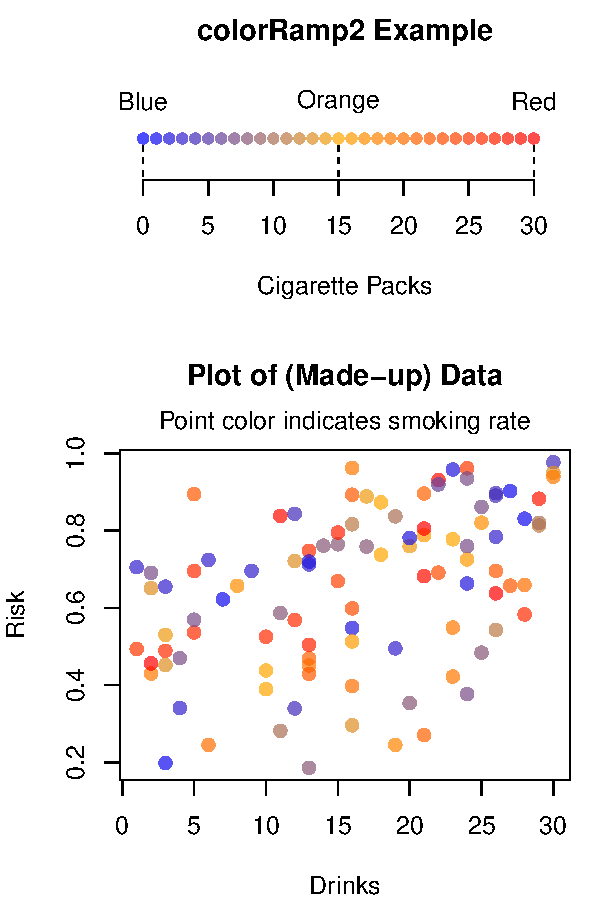
\includegraphics[width=\maxwidth]{figure/unnamed-chunk-172-1} 

\end{knitrout}
\end{tiny}
\label{fig:colorramp}
\end{marginfigure}


The best way to explain how \texttt{colorRamp2} works is by giving you an example. Let's say that you want to want to plot data showing the relationship between the number of drinks someone has on average per week and the resulting risk of some adverse health effect. Further, let's say you want to color the points as a function of the number of packs of cigarettes per week that person smokes, where a value of 0 packs is colored Blue, 10 packs is Orange, and 30 packs is Red. Moreover, you want the values in between these \textit{break points} of 0, 10 and 30 to be a mix of the colors. For example, the value of 5 (half way between 0 and 10) should be an equal mix of Blue and Orange.

\texttt{colorRamp2} allows you to do exactly this. The function has three arguments:

\begin{itemize}
  \item \texttt{breaks}: A vector indicating the break points
  \item \texttt{colors}: A vector of colors corresponding to each value in \texttt{breaks}
  \item \texttt{transparency}: A value between 0 and 1 indicating the transparency (1 means fully transparent)
\end{itemize}

When you run the function, the function will actually \textit{return} another function that you can then use to generate colors. Once you store the resulting function as an object (something like \texttt{my.color.fun} You can then apply this new function on numerical data (in our example, the number of cigarettes someone smokes) to obtain the correct color for each data point. 

For example, let's create the color ramp function for our smoking data points. I'll use \texttt{colorRamp2} to create a function that I'll call \texttt{smoking.colors} which takes a number as an argument, and returns the corresponding color:

\begin{knitrout}
\definecolor{shadecolor}{rgb}{0.969, 0.969, 0.969}\color{fgcolor}\begin{kframe}
\begin{alltt}
\hlstd{smoking.colors} \hlkwb{<-} \hlkwd{colorRamp2}\hlstd{(}\hlkwc{breaks} \hlstd{=} \hlkwd{c}\hlstd{(}\hlnum{0}\hlstd{,} \hlnum{15}\hlstd{,} \hlnum{30}\hlstd{),}
                  \hlkwc{colors} \hlstd{=} \hlkwd{c}\hlstd{(}\hlstr{"blue"}\hlstd{,} \hlstr{"orange"}\hlstd{,} \hlstr{"red"}\hlstd{),}
                  \hlkwc{transparency} \hlstd{=} \hlnum{.3}
                  \hlstd{)}

\hlkwd{smoking.colors}\hlstd{(}\hlnum{0}\hlstd{)} \hlcom{# Equivalent to blue}
\end{alltt}
\begin{verbatim}
## [1] "#0000FFB3"
\end{verbatim}
\begin{alltt}
\hlkwd{smoking.colors}\hlstd{(}\hlnum{20}\hlstd{)} \hlcom{# Mix of orange and red}
\end{alltt}
\begin{verbatim}
## [1] "#FF6E00B3"
\end{verbatim}
\end{kframe}
\end{knitrout}

To see this function in action, check out the the margin Figure~\ref{fig:colorramp} for an example, and check out the help menu \texttt{?colorRamp2} for more information and examples.

\subsection{Stealing any color from your screen with a kuler}

One of my favorite tricks for getting great colors in R is to use a \textit{color kuler}. A color kuler is a tool that allows you to determine the exact RGB values for a color on a screen. For example, let's say that you wanted to use the exact colors used in the Google logo. To do this, you need to use an app that allows you to pick colors off your computer screen. On a Mac, you can use the program called "Digital Color Meter." If you then move your mouse over the color you want, the software will tell you the exact RGB values of that color. In the image below, you can see me figuring out that the RGB value of the G in Google is R: 19, G: 72, B: 206. Using this method, I figured out the four colors of Google! Check out the margin Figure~\ref{fig:googlecolors} for the grand result.

\begin{marginfigure}
\begin{tiny}
\begin{knitrout}
\definecolor{shadecolor}{rgb}{0.969, 0.969, 0.969}\color{fgcolor}\begin{kframe}
\begin{alltt}
\hlstd{google.colors} \hlkwb{<-} \hlkwd{c}\hlstd{(}
  \hlkwd{rgb}\hlstd{(}\hlnum{19}\hlstd{,} \hlnum{72}\hlstd{,} \hlnum{206}\hlstd{,} \hlkwc{maxColorValue} \hlstd{=} \hlnum{255}\hlstd{),}
  \hlkwd{rgb}\hlstd{(}\hlnum{206}\hlstd{,} \hlnum{45}\hlstd{,} \hlnum{35}\hlstd{,} \hlkwc{maxColorValue} \hlstd{=} \hlnum{255}\hlstd{),}
  \hlkwd{rgb}\hlstd{(}\hlnum{253}\hlstd{,} \hlnum{172}\hlstd{,} \hlnum{10}\hlstd{,} \hlkwc{maxColorValue} \hlstd{=} \hlnum{255}\hlstd{),}
  \hlkwd{rgb}\hlstd{(}\hlnum{18}\hlstd{,} \hlnum{140}\hlstd{,} \hlnum{70}\hlstd{,} \hlkwc{maxColorValue} \hlstd{=} \hlnum{255}\hlstd{))}

\hlkwd{par}\hlstd{(}\hlkwc{mar} \hlstd{=} \hlkwd{rep}\hlstd{(}\hlnum{0}\hlstd{,} \hlnum{4}\hlstd{))}

\hlkwd{plot}\hlstd{(}\hlnum{1}\hlstd{,} \hlkwc{xlim} \hlstd{=} \hlkwd{c}\hlstd{(}\hlnum{0}\hlstd{,} \hlnum{7}\hlstd{),} \hlkwc{ylim} \hlstd{=} \hlkwd{c}\hlstd{(}\hlnum{0}\hlstd{,} \hlnum{1}\hlstd{),}
     \hlkwc{xlab} \hlstd{=} \hlstr{""}\hlstd{,} \hlkwc{ylab} \hlstd{=} \hlstr{""}\hlstd{,} \hlkwc{xaxt} \hlstd{=} \hlstr{"n"}\hlstd{,} \hlkwc{yaxt} \hlstd{=} \hlstr{"n"}\hlstd{,}
     \hlkwc{type} \hlstd{=} \hlstr{"n"}\hlstd{,} \hlkwc{bty} \hlstd{=} \hlstr{"n"}
     \hlstd{)}

\hlkwd{points}\hlstd{(}\hlnum{1}\hlopt{:}\hlnum{6}\hlstd{,} \hlkwd{rep}\hlstd{(}\hlnum{.5}\hlstd{,} \hlnum{6}\hlstd{),}
       \hlkwc{pch} \hlstd{=} \hlkwd{c}\hlstd{(}\hlnum{15}\hlstd{,} \hlnum{16}\hlstd{,} \hlnum{16}\hlstd{,} \hlnum{17}\hlstd{,} \hlnum{18}\hlstd{,} \hlnum{15}\hlstd{),}
       \hlkwc{col} \hlstd{= google.colors[}\hlkwd{c}\hlstd{(}\hlnum{1}\hlstd{,} \hlnum{2}\hlstd{,} \hlnum{3}\hlstd{,} \hlnum{1}\hlstd{,} \hlnum{4}\hlstd{,} \hlnum{2}\hlstd{)],}
       \hlkwc{cex} \hlstd{=} \hlnum{2.5}\hlstd{)}

\hlkwd{text}\hlstd{(}\hlnum{3.5}\hlstd{,} \hlnum{.7}\hlstd{,} \hlstr{"Look familiar?"}\hlstd{,} \hlkwc{cex} \hlstd{=} \hlnum{1.5}\hlstd{)}
\end{alltt}
\end{kframe}
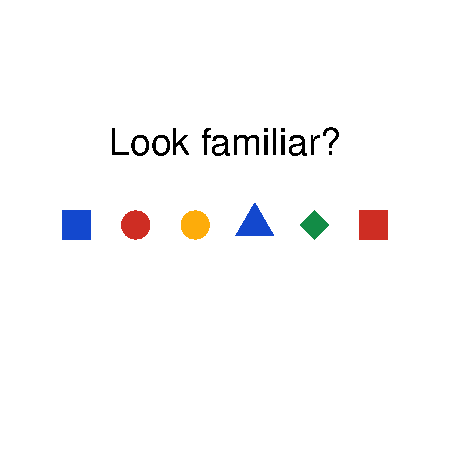
\includegraphics[width=\maxwidth]{figure/unnamed-chunk-174-1} 

\end{knitrout}
\end{tiny}
\label{fig:googlecolors}
\caption{Stealing colors from the internet. Not illegal (yet).}
\end{marginfigure}

\begin{figure}
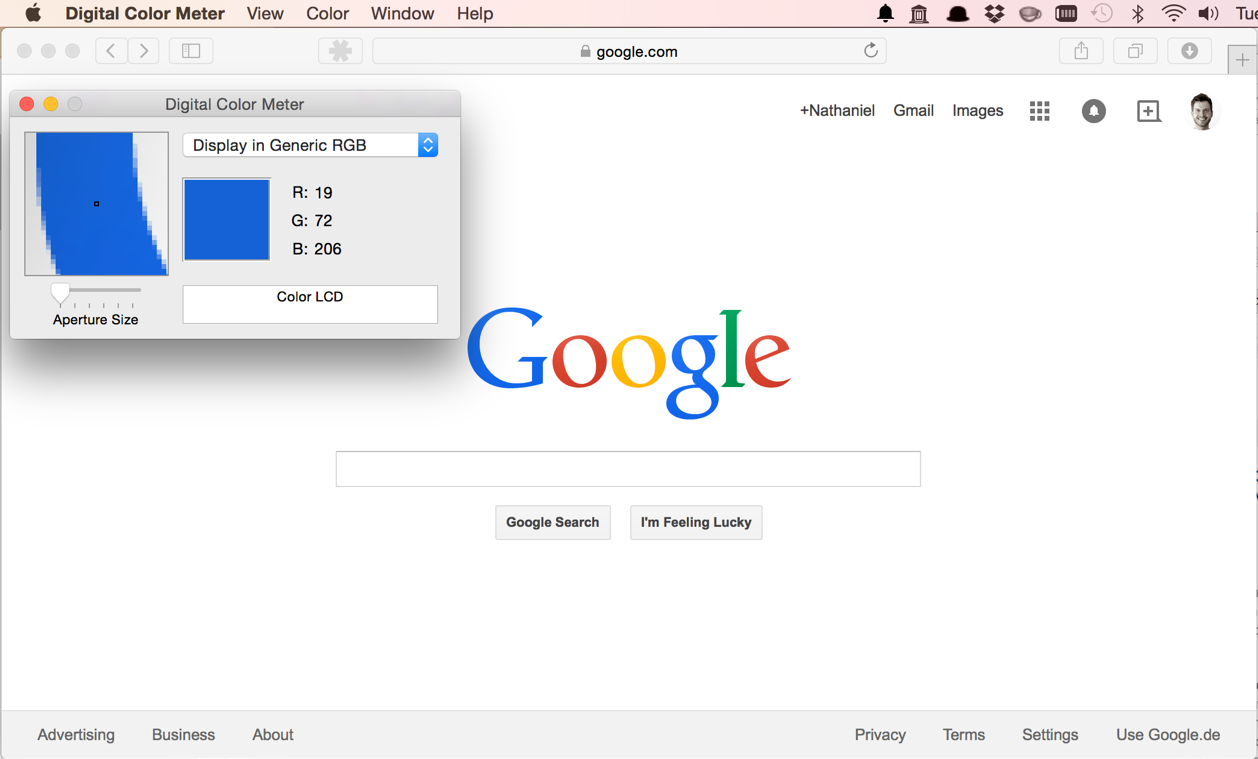
\includegraphics[width=\linewidth]{/Users/Nathaniel/Dropbox/Git/YaRrr_Book/media/kuler.png}
\end{figure}


\pagebreak

\section{Plot margins}

\begin{marginfigure}
\begin{tiny}
\begin{knitrout}
\definecolor{shadecolor}{rgb}{0.969, 0.969, 0.969}\color{fgcolor}\begin{kframe}
\begin{alltt}
\hlkwd{par}\hlstd{(}\hlkwc{mar} \hlstd{=} \hlkwd{rep}\hlstd{(}\hlnum{8}\hlstd{,} \hlnum{4}\hlstd{))}

\hlstd{x.vals} \hlkwb{<-} \hlkwd{rnorm}\hlstd{(}\hlnum{500}\hlstd{)}
\hlstd{y.vals} \hlkwb{<-} \hlstd{x.vals} \hlopt{+} \hlkwd{rnorm}\hlstd{(}\hlnum{500}\hlstd{,} \hlkwc{sd} \hlstd{=} \hlnum{.5}\hlstd{)}

\hlkwd{plot}\hlstd{(x.vals, y.vals,} \hlkwc{xlim} \hlstd{=} \hlkwd{c}\hlstd{(}\hlopt{-}\hlnum{2}\hlstd{,} \hlnum{2}\hlstd{),} \hlkwc{ylim} \hlstd{=} \hlkwd{c}\hlstd{(}\hlopt{-}\hlnum{2}\hlstd{,} \hlnum{2}\hlstd{),}
     \hlkwc{main} \hlstd{=} \hlstr{""}\hlstd{,} \hlkwc{xlab} \hlstd{=} \hlstr{""}\hlstd{,} \hlkwc{ylab} \hlstd{=} \hlstr{""}\hlstd{,} \hlkwc{xaxt} \hlstd{=} \hlstr{"n"}\hlstd{,}
     \hlkwc{yaxt} \hlstd{=} \hlstr{"n"}\hlstd{,} \hlkwc{bty} \hlstd{=} \hlstr{"n"}\hlstd{,} \hlkwc{pch} \hlstd{=} \hlnum{16}\hlstd{,} \hlkwc{col} \hlstd{=} \hlkwd{gray}\hlstd{(}\hlnum{.5}\hlstd{,} \hlkwc{alpha} \hlstd{=} \hlnum{.2}\hlstd{))}

\hlkwd{axis}\hlstd{(}\hlnum{1}\hlstd{,} \hlkwc{at} \hlstd{=} \hlkwd{seq}\hlstd{(}\hlopt{-}\hlnum{2}\hlstd{,} \hlnum{2}\hlstd{,} \hlnum{.5}\hlstd{),} \hlkwc{col.axis} \hlstd{=} \hlkwd{gray}\hlstd{(}\hlnum{.8}\hlstd{),} \hlkwc{col} \hlstd{=} \hlkwd{gray}\hlstd{(}\hlnum{.8}\hlstd{))}
\hlkwd{axis}\hlstd{(}\hlnum{2}\hlstd{,} \hlkwc{at} \hlstd{=} \hlkwd{seq}\hlstd{(}\hlopt{-}\hlnum{2}\hlstd{,} \hlnum{2}\hlstd{,} \hlnum{.5}\hlstd{),} \hlkwc{col.axis} \hlstd{=} \hlkwd{gray}\hlstd{(}\hlnum{.8}\hlstd{),} \hlkwc{col} \hlstd{=} \hlkwd{gray}\hlstd{(}\hlnum{.8}\hlstd{))}

\hlkwd{par}\hlstd{(}\hlkwc{new} \hlstd{= T)}
\hlkwd{par}\hlstd{(}\hlkwc{mar} \hlstd{=} \hlkwd{rep}\hlstd{(}\hlnum{0}\hlstd{,} \hlnum{4}\hlstd{))}
\hlkwd{plot}\hlstd{(}\hlnum{1}\hlstd{,} \hlkwc{xlim} \hlstd{=} \hlkwd{c}\hlstd{(}\hlnum{0}\hlstd{,} \hlnum{1}\hlstd{),} \hlkwc{ylim} \hlstd{=} \hlkwd{c}\hlstd{(}\hlnum{0}\hlstd{,} \hlnum{1}\hlstd{),} \hlkwc{type} \hlstd{=}\hlstr{"n"}\hlstd{,}
     \hlkwc{main} \hlstd{=} \hlstr{""}\hlstd{,} \hlkwc{bty} \hlstd{=} \hlstr{"n"}\hlstd{,} \hlkwc{xlab} \hlstd{=} \hlstr{""}\hlstd{,} \hlkwc{ylab} \hlstd{=} \hlstr{""}\hlstd{,} \hlkwc{xaxt} \hlstd{=} \hlstr{"n"}\hlstd{,} \hlkwc{yaxt} \hlstd{=} \hlstr{"n"}\hlstd{)}

\hlkwd{rect}\hlstd{(}\hlnum{0}\hlstd{,} \hlnum{0}\hlstd{,} \hlnum{1}\hlstd{,} \hlnum{1}\hlstd{)}

\hlkwd{rect}\hlstd{(}\hlnum{.21}\hlstd{,} \hlnum{.22}\hlstd{,} \hlnum{.85}\hlstd{,} \hlnum{.8}\hlstd{,} \hlkwc{lty} \hlstd{=} \hlnum{2}\hlstd{)}

\hlkwd{arrows}\hlstd{(}\hlkwd{c}\hlstd{(}\hlnum{.5}\hlstd{,} \hlnum{.5}\hlstd{,} \hlnum{0}\hlstd{,} \hlnum{.85}\hlstd{),}
       \hlkwd{c}\hlstd{(}\hlnum{.8}\hlstd{,} \hlnum{.22}\hlstd{,} \hlnum{.5}\hlstd{,} \hlnum{.5}\hlstd{),}
       \hlkwd{c}\hlstd{(}\hlnum{.5}\hlstd{,} \hlnum{.5}\hlstd{,} \hlnum{.21}\hlstd{,} \hlnum{1}\hlstd{),}
       \hlkwd{c}\hlstd{(}\hlnum{1}\hlstd{,} \hlnum{0}\hlstd{,} \hlnum{.5}\hlstd{,} \hlnum{.5}\hlstd{),}
       \hlkwc{code} \hlstd{=} \hlnum{3}\hlstd{,} \hlkwc{length} \hlstd{=} \hlnum{.1}
       \hlstd{)}

\hlkwd{text}\hlstd{(}\hlkwd{c}\hlstd{(}\hlnum{.5}\hlstd{,} \hlnum{.5}\hlstd{,} \hlnum{.09}\hlstd{,} \hlnum{.93}\hlstd{),}
     \hlkwd{c}\hlstd{(}\hlnum{.88}\hlstd{,} \hlnum{.11}\hlstd{,} \hlnum{.5}\hlstd{,} \hlnum{.5}\hlstd{),}
     \hlkwc{labels} \hlstd{=} \hlkwd{c}\hlstd{(}\hlstr{"mar[1]"}\hlstd{,} \hlstr{"mar[2]"}\hlstd{,} \hlstr{"mar[3]"}\hlstd{,} \hlstr{"mar[4]"}\hlstd{),}
     \hlkwc{pos} \hlstd{=} \hlkwd{c}\hlstd{(}\hlnum{2}\hlstd{,} \hlnum{2}\hlstd{,} \hlnum{1}\hlstd{,} \hlnum{1}\hlstd{)}
     \hlstd{)}

\hlkwd{text}\hlstd{(}\hlnum{.7}\hlstd{,} \hlnum{.9}\hlstd{,} \hlstr{"This is Margin Text\textbackslash{}nMade with mtext()"}\hlstd{)}
\end{alltt}
\end{kframe}
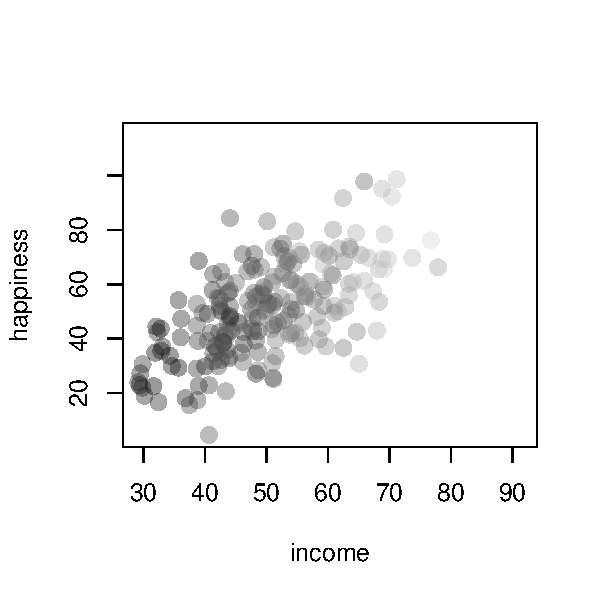
\includegraphics[width=\maxwidth]{figure/unnamed-chunk-175-1} 

\end{knitrout}
\end{tiny}
\label{fig:marplot}
\end{marginfigure}


All plots in R have margins surrounding them that separate the main plotting space from the area where the axes, labels and additional text lie.. To visualize how R creates plot margins, look at margin Figure~\ref{fig:marplot}.

You can adjust the size of the margins by specifying a margin parameter using the syntax \texttt{par(mar = c(a, b, c, d))} before you execute your first high-level plotting function, where a, b, c and d are the size of the margins on the bottom, left, top, and right of the plot. Let's see how this works by creating two plots with different margins:

In the plot on the left, I'll set the margins to 3 on all sides. In the plot on the right, I'll set the margins to 6 on all sides.

\begin{footnotesize}
\begin{knitrout}
\definecolor{shadecolor}{rgb}{0.969, 0.969, 0.969}\color{fgcolor}\begin{kframe}
\begin{alltt}
\hlkwd{par}\hlstd{(}\hlkwc{mfrow} \hlstd{=} \hlkwd{c}\hlstd{(}\hlnum{1}\hlstd{,} \hlnum{2}\hlstd{))} \hlcom{# Put plots next to each other}

\hlcom{# First Plot}
\hlkwd{par}\hlstd{(}\hlkwc{mar} \hlstd{=} \hlkwd{rep}\hlstd{(}\hlnum{2}\hlstd{,} \hlnum{4}\hlstd{))} \hlcom{# Set the margin on all sides to 2}
\hlkwd{plot}\hlstd{(}\hlnum{1}\hlopt{:}\hlnum{10}\hlstd{)}
\hlkwd{mtext}\hlstd{(}\hlstr{"Small Margins"}\hlstd{,} \hlkwc{side} \hlstd{=} \hlnum{3}\hlstd{,} \hlkwc{line} \hlstd{=} \hlnum{1}\hlstd{,} \hlkwc{cex} \hlstd{=} \hlnum{1.2}\hlstd{)}

\hlcom{# Second Plot}
\hlkwd{par}\hlstd{(}\hlkwc{mar} \hlstd{=} \hlkwd{rep}\hlstd{(}\hlnum{6}\hlstd{,} \hlnum{4}\hlstd{))} \hlcom{# Set the margin on all sides to 6}
\hlkwd{plot}\hlstd{(}\hlnum{1}\hlopt{:}\hlnum{10}\hlstd{)}
\hlkwd{mtext}\hlstd{(}\hlstr{"Large Margins"}\hlstd{,} \hlkwc{side} \hlstd{=} \hlnum{3}\hlstd{,} \hlkwc{line} \hlstd{=} \hlnum{1}\hlstd{,} \hlkwc{cex} \hlstd{=} \hlnum{1.2}\hlstd{)}
\end{alltt}
\end{kframe}
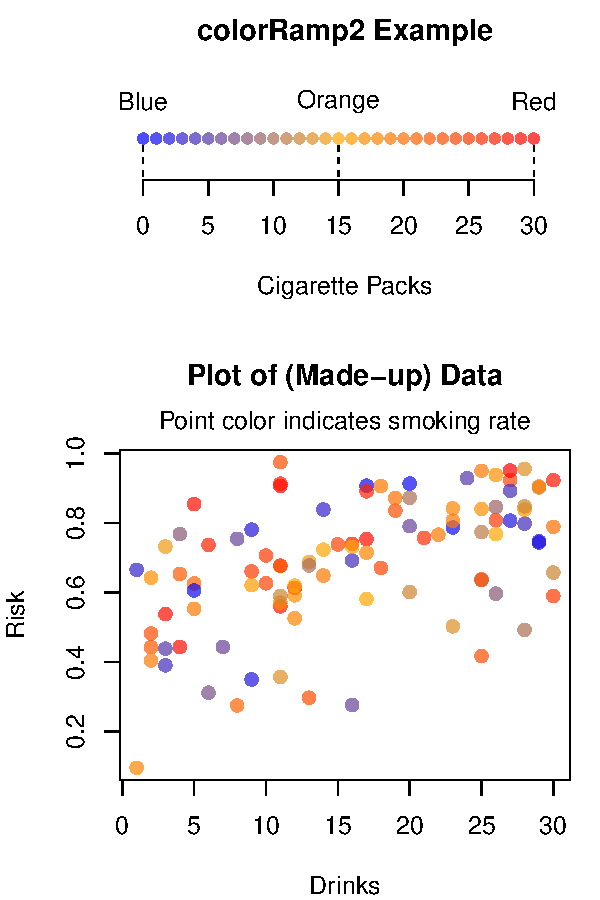
\includegraphics[width=\maxwidth]{figure/unnamed-chunk-176-1} 

\end{knitrout}
\end{footnotesize}

\marginnote{The default value for \texttt{mar} is \texttt{c(5.1, 4.1, 4.1, 2.1)}}

You'll notice that the margins are so small in the first plot that you can't even see the axis labels, while in the second plot there is plenty (probably too much) white space around the plotting region.

In addition to using the \texttt{mar} parameter, you can also specify margin sizes with the \text{mai} parameter. This acts just like \texttt{mar} except that the values for \texttt{mai} set the margin size in inches.


\pagebreak

\section{Arranging multiple plots with \texttt{par(mfrow)} and \texttt{layout}}

R makes it easy to arrange multiple plots in the same plotting space. The most common ways to do this is with the \texttt{par(mfrow)} parameter, and the \texttt{layout()} function. Let's go over each in turn:

\subsection{Simple plot layouts with par(mfrow) and par(mfcol)}

\begin{marginfigure}
\begin{tiny}
\begin{knitrout}
\definecolor{shadecolor}{rgb}{0.969, 0.969, 0.969}\color{fgcolor}\begin{kframe}
\begin{alltt}
\hlkwd{par}\hlstd{(}\hlkwc{mfrow} \hlstd{=} \hlkwd{c}\hlstd{(}\hlnum{3}\hlstd{,} \hlnum{3}\hlstd{))}
\hlkwd{par}\hlstd{(}\hlkwc{mar} \hlstd{=} \hlkwd{rep}\hlstd{(}\hlnum{2.5}\hlstd{,} \hlnum{4}\hlstd{))}

\hlkwa{for}\hlstd{(i} \hlkwa{in} \hlnum{1}\hlopt{:}\hlnum{9}\hlstd{) \{} \hlcom{# Loop across plots}

\hlcom{# Generate data  }
\hlstd{x} \hlkwb{<-} \hlkwd{rnorm}\hlstd{(}\hlnum{100}\hlstd{)}
\hlstd{y} \hlkwb{<-} \hlstd{x} \hlopt{+} \hlkwd{rnorm}\hlstd{(}\hlnum{100}\hlstd{)}

\hlcom{# Plot data}
  \hlkwd{plot}\hlstd{(x, y,} \hlkwc{xlim} \hlstd{=} \hlkwd{c}\hlstd{(}\hlopt{-}\hlnum{2}\hlstd{,} \hlnum{2}\hlstd{),} \hlkwc{ylim} \hlstd{=} \hlkwd{c}\hlstd{(}\hlopt{-}\hlnum{2}\hlstd{,} \hlnum{2}\hlstd{),}
       \hlkwc{col.main} \hlstd{=} \hlstr{"gray"}\hlstd{,}
       \hlkwc{pch} \hlstd{=} \hlnum{16}\hlstd{,} \hlkwc{col} \hlstd{=} \hlkwd{gray}\hlstd{(}\hlnum{.0}\hlstd{,} \hlkwc{alpha} \hlstd{=} \hlnum{.1}\hlstd{),}
       \hlkwc{xaxt} \hlstd{=} \hlstr{"n"}\hlstd{,} \hlkwc{yaxt} \hlstd{=} \hlstr{"n"}
       \hlstd{)}

\hlcom{# Add a regression line for fun}
\hlkwd{abline}\hlstd{(}\hlkwd{lm}\hlstd{(y} \hlopt{~} \hlstd{x),} \hlkwc{col} \hlstd{=} \hlstr{"gray"}\hlstd{,} \hlkwc{lty} \hlstd{=} \hlnum{2}\hlstd{)}


\hlcom{# Add gray axes}
\hlkwd{axis}\hlstd{(}\hlnum{1}\hlstd{,} \hlkwc{col.axis} \hlstd{=} \hlstr{"gray"}\hlstd{,}
     \hlkwc{col.lab} \hlstd{=} \hlkwd{gray}\hlstd{(}\hlnum{.1}\hlstd{),} \hlkwc{col} \hlstd{=} \hlstr{"gray"}\hlstd{)}

\hlkwd{axis}\hlstd{(}\hlnum{2}\hlstd{,} \hlkwc{col.axis} \hlstd{=} \hlstr{"gray"}\hlstd{,}
     \hlkwc{col.lab} \hlstd{=} \hlkwd{gray}\hlstd{(}\hlnum{.1}\hlstd{),} \hlkwc{col} \hlstd{=} \hlstr{"gray"}\hlstd{)}

\hlcom{# Add large index text}
\hlkwd{text}\hlstd{(}\hlnum{0}\hlstd{,} \hlnum{0}\hlstd{, i,} \hlkwc{cex} \hlstd{=} \hlnum{7}\hlstd{)}

\hlcom{# Create box around border}
\hlkwd{box}\hlstd{(}\hlkwc{which} \hlstd{=} \hlstr{"figure"}\hlstd{,} \hlkwc{lty} \hlstd{=} \hlnum{2}\hlstd{)}

\hlstd{\}}
\end{alltt}
\end{kframe}
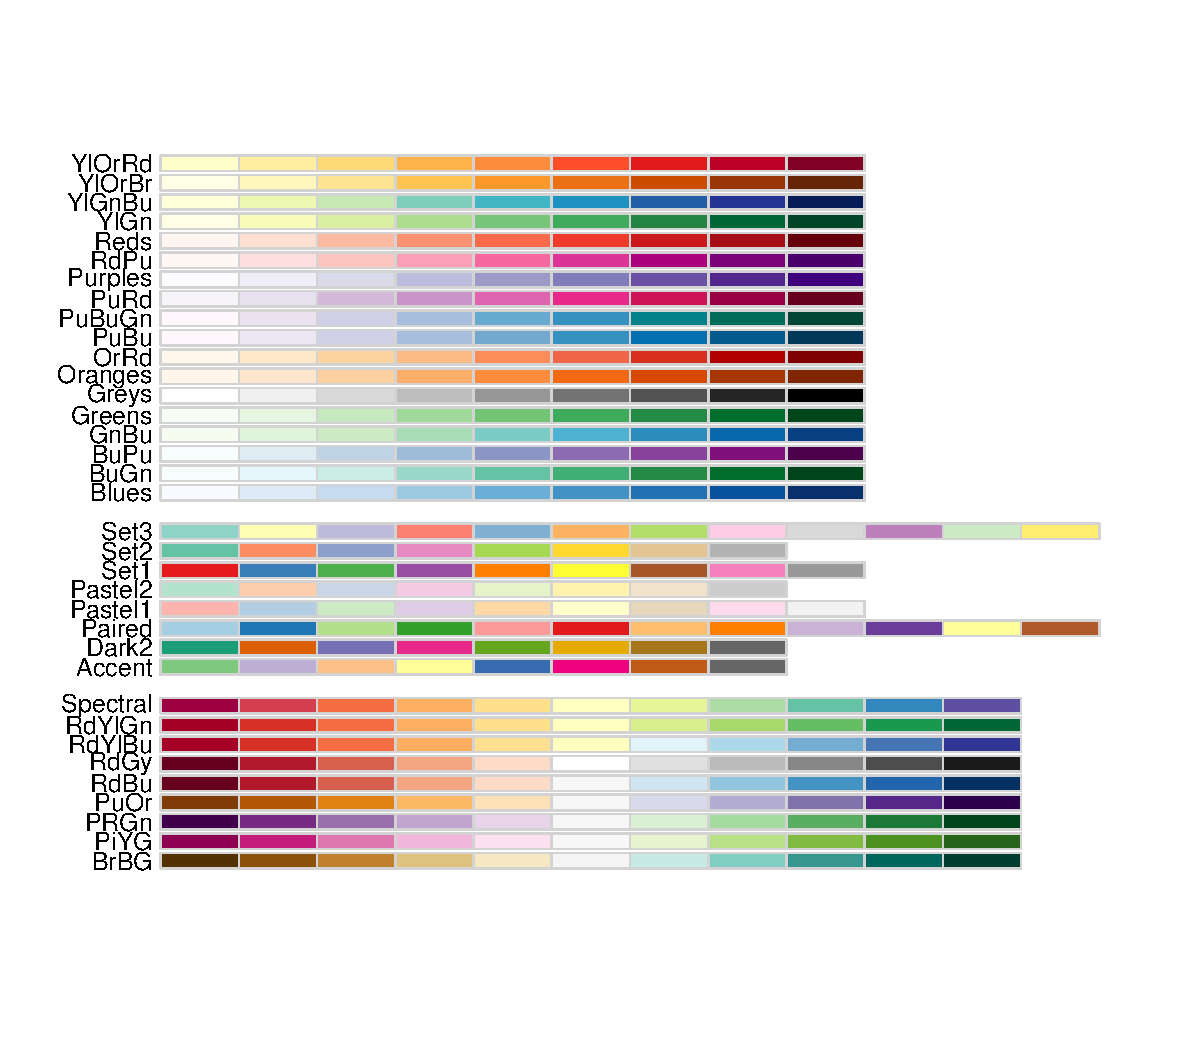
\includegraphics[width=\maxwidth]{figure/unnamed-chunk-177-1} 

\end{knitrout}
\end{tiny}
\caption{A matrix of plotting regions created by \texttt{par(mfrow = c(3, 3))}}
\label{fig:mfrow}
\end{marginfigure}


The \texttt{mfrow} and \texttt{mfcol} parameters allow you to create a matrix of plots in one plotting space. Both parameters take a vector of length two as an argument, corresponding to the number of rows and columns in the resulting plotting matrix. For example, the following code sets up a 3 x 3 plotting matrix.

\begin{knitrout}
\definecolor{shadecolor}{rgb}{0.969, 0.969, 0.969}\color{fgcolor}\begin{kframe}
\begin{alltt}
\hlkwd{par}\hlstd{(}\hlkwc{mfrow} \hlstd{=} \hlkwd{c}\hlstd{(}\hlnum{3}\hlstd{,} \hlnum{3}\hlstd{))} \hlcom{# Create a 3 x 3 plotting matrix}
\end{alltt}
\end{kframe}
\end{knitrout}

When you execute this code, you won't see anything happen. However, when you execute your first high-level plotting command, you'll see that the plot will show up in the space reserved for the first plot (the top left). When you execute a second high-level plotting command, R will place that plot in the second place in the plotting matrix - either the top middle (if using \texttt{par(mfrow)} or the left middle (if using \texttt{par(mfcol)}). As you continue to add high-level plots, R will continue to fill the plotting matrix.

So what's the difference between \texttt{par(mfrow)} and \texttt{par(mfcol)}? The only difference is that while \texttt{par(mfrow)} puts sequential plots into the plotting matrix by row, \texttt{par(mfcol)} will fill them by column.

When you are finished using a plotting matrix, be sure to reset the plotting parameter back to its default state:

\begin{knitrout}
\definecolor{shadecolor}{rgb}{0.969, 0.969, 0.969}\color{fgcolor}\begin{kframe}
\begin{alltt}
\hlkwd{par}\hlstd{(}\hlkwc{mfrow} \hlstd{=} \hlkwd{c}\hlstd{(}\hlnum{1}\hlstd{,} \hlnum{1}\hlstd{))}
\end{alltt}
\end{kframe}
\end{knitrout}

If you don't reset the \texttt{mfrow} parameter, R will continue creating new plotting matrices.

\subsection{Complex plot layouts with \texttt{layout()}}

While \texttt{par(mfrow)} allows you to create matrices of plots, it does not allow you to create plots of different sizes. In order to arrange plots in different sized plotting spaces, you need to use the \texttt{layout()} function. Unlike \texttt{par(mfrow)}, \texttt{layout} is not a plotting parameter, rather it is a function all on its own. Let's go through the main arguments of \texttt{layout()}:

\newfun{layout(mat, widths, heights)}

\begin{itemize}

  \item \texttt{mat}: A matrix indicating the location of the next N figures in the global plotting space. Each value in the matrix must be 0 or a positive integer. R will plot the first plot in the entries of the matrix with 1, the second plot in the entries with 2,...
  \item \texttt{widths}: A vector of values for the widths of the columns of the plotting space.
  \item \texttt{heights}: A vector of values for the heights of the rows of the plotting space.

\end{itemize}

The \texttt{layout()} function can be a bit confusing at first, so I think it's best to start with an example. Let's say you want to place histograms next to a scatterplot: Let's do this using layout

\begin{marginfigure}
\begin{tiny}
\begin{knitrout}
\definecolor{shadecolor}{rgb}{0.969, 0.969, 0.969}\color{fgcolor}\begin{kframe}
\begin{alltt}
\hlstd{layout.matrix} \hlkwb{<-} \hlkwd{matrix}\hlstd{(}\hlkwd{c}\hlstd{(}\hlnum{2}\hlstd{,} \hlnum{1}\hlstd{,} \hlnum{0}\hlstd{,} \hlnum{3}\hlstd{),} \hlkwc{nrow} \hlstd{=} \hlnum{2}\hlstd{,} \hlkwc{ncol} \hlstd{=} \hlnum{2}\hlstd{)}

\hlkwd{layout}\hlstd{(}\hlkwc{mat} \hlstd{= layout.matrix,}
       \hlkwc{heights} \hlstd{=} \hlkwd{c}\hlstd{(}\hlnum{1}\hlstd{,} \hlnum{2}\hlstd{),} \hlcom{# Heights of the two rows}
       \hlkwc{widths} \hlstd{=} \hlkwd{c}\hlstd{(}\hlnum{2}\hlstd{,} \hlnum{2}\hlstd{)} \hlcom{# Widths of the two columns}
       \hlstd{)}

\hlkwd{layout.show}\hlstd{(}\hlnum{3}\hlstd{)}
\end{alltt}
\end{kframe}
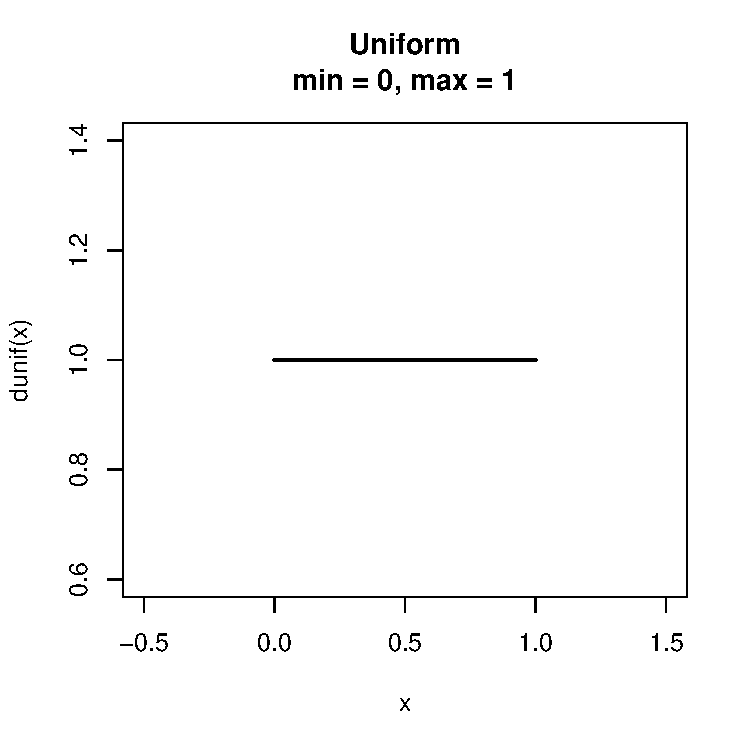
\includegraphics[width=\maxwidth]{figure/unnamed-chunk-180-1} 

\end{knitrout}
\end{tiny}
\caption{A plotting layout created by setting a layout matrix and specific heights and widths.}
\label{fig:layout}
\end{marginfigure}

We'll begin by creating the \textit{layout matrix}, this matrix will tell R in which order to create the plots:

\begin{knitrout}
\definecolor{shadecolor}{rgb}{0.969, 0.969, 0.969}\color{fgcolor}\begin{kframe}
\begin{alltt}
\hlstd{layout.matrix} \hlkwb{<-} \hlkwd{matrix}\hlstd{(}\hlkwd{c}\hlstd{(}\hlnum{0}\hlstd{,} \hlnum{2}\hlstd{,} \hlnum{3}\hlstd{,} \hlnum{1}\hlstd{),} \hlkwc{nrow} \hlstd{=} \hlnum{2}\hlstd{,} \hlkwc{ncol} \hlstd{=} \hlnum{2}\hlstd{)}
\hlstd{layout.matrix}
\end{alltt}
\begin{verbatim}
##      [,1] [,2]
## [1,]    0    3
## [2,]    2    1
\end{verbatim}
\end{kframe}
\end{knitrout}

Looking at the values of \texttt{layout.matrix}, you can see that we've told R to put the first plot in the bottom right, the second plot on the bottom left, and the third plot in the top right. Because we put a 0 in the first element, R knows that we don't plan to put anything in the top left area.

Now, because our layout matrix has two rows and two columns, we need to set the widths and heights of the two columns. We do this using a numeric vector of length 2. I'll set the heights of the two rows to 1 and 2 respectively, and the widths of the columns to 1 and 2 respectively. Now, when I run the code \texttt{layout.show(3)}, R will show us the plotting region we set up (see margin Figure~\ref{fig:layout})

Now we're ready to put the plots together

\begin{footnotesize}
\begin{knitrout}
\definecolor{shadecolor}{rgb}{0.969, 0.969, 0.969}\color{fgcolor}\begin{kframe}
\begin{alltt}
\hlstd{layout.matrix} \hlkwb{<-} \hlkwd{matrix}\hlstd{(}\hlkwd{c}\hlstd{(}\hlnum{2}\hlstd{,} \hlnum{1}\hlstd{,} \hlnum{0}\hlstd{,} \hlnum{3}\hlstd{),} \hlkwc{nrow} \hlstd{=} \hlnum{2}\hlstd{,} \hlkwc{ncol} \hlstd{=} \hlnum{2}\hlstd{)}

\hlkwd{layout}\hlstd{(}\hlkwc{mat} \hlstd{= layout.matrix,}
       \hlkwc{heights} \hlstd{=} \hlkwd{c}\hlstd{(}\hlnum{1}\hlstd{,} \hlnum{2}\hlstd{),} \hlcom{# Heights of the two rows}
       \hlkwc{widths} \hlstd{=} \hlkwd{c}\hlstd{(}\hlnum{2}\hlstd{,} \hlnum{1}\hlstd{)} \hlcom{# Widths of the two columns}
       \hlstd{)}

\hlstd{x.vals} \hlkwb{<-} \hlkwd{rnorm}\hlstd{(}\hlnum{100}\hlstd{,} \hlkwc{mean} \hlstd{=} \hlnum{100}\hlstd{,} \hlkwc{sd} \hlstd{=} \hlnum{10}\hlstd{)}
\hlstd{y.vals} \hlkwb{<-} \hlstd{x.vals} \hlopt{+} \hlkwd{rnorm}\hlstd{(}\hlnum{100}\hlstd{,} \hlkwc{mean} \hlstd{=} \hlnum{0}\hlstd{,} \hlkwc{sd} \hlstd{=} \hlnum{10}\hlstd{)}

\hlcom{# Plot 1: Scatterplot}
\hlkwd{par}\hlstd{(}\hlkwc{mar} \hlstd{=} \hlkwd{c}\hlstd{(}\hlnum{5}\hlstd{,} \hlnum{4}\hlstd{,} \hlnum{0}\hlstd{,} \hlnum{0}\hlstd{))}
\hlkwd{plot}\hlstd{(x.vals, y.vals)}
\hlkwd{abline}\hlstd{(}\hlkwc{h} \hlstd{=} \hlkwd{median}\hlstd{(y.vals),} \hlkwc{lty} \hlstd{=} \hlnum{1}\hlstd{,} \hlkwc{col} \hlstd{=} \hlstr{"gray"}\hlstd{)}
\hlkwd{abline}\hlstd{(}\hlkwc{v} \hlstd{=} \hlkwd{median}\hlstd{(x.vals),} \hlkwc{lty} \hlstd{=} \hlnum{1}\hlstd{,} \hlkwc{col} \hlstd{=} \hlstr{"gray"}\hlstd{)}


\hlcom{# Plot 2: X boxplot}
\hlkwd{par}\hlstd{(}\hlkwc{mar} \hlstd{=} \hlkwd{c}\hlstd{(}\hlnum{0}\hlstd{,} \hlnum{4}\hlstd{,} \hlnum{0}\hlstd{,} \hlnum{0}\hlstd{))}
\hlkwd{boxplot}\hlstd{(x.vals,} \hlkwc{xaxt} \hlstd{=} \hlstr{"n"}\hlstd{,}
        \hlkwc{yaxt} \hlstd{=} \hlstr{"n"}\hlstd{,} \hlkwc{bty} \hlstd{=} \hlstr{"n"}\hlstd{,} \hlkwc{yaxt} \hlstd{=} \hlstr{"n"}\hlstd{,}
        \hlkwc{col} \hlstd{=} \hlstr{"white"}\hlstd{,} \hlkwc{frame} \hlstd{= F,} \hlkwc{horizontal} \hlstd{= T)}

\hlcom{# Plot 3: Y boxplot}
\hlkwd{par}\hlstd{(}\hlkwc{mar} \hlstd{=} \hlkwd{c}\hlstd{(}\hlnum{5}\hlstd{,} \hlnum{0}\hlstd{,} \hlnum{0}\hlstd{,} \hlnum{0}\hlstd{))}
\hlkwd{boxplot}\hlstd{(y.vals,} \hlkwc{xaxt} \hlstd{=} \hlstr{"n"}\hlstd{,}
        \hlkwc{yaxt} \hlstd{=} \hlstr{"n"}\hlstd{,} \hlkwc{bty} \hlstd{=} \hlstr{"n"}\hlstd{,} \hlkwc{yaxt} \hlstd{=} \hlstr{"n"}\hlstd{,}
        \hlkwc{col} \hlstd{=} \hlstr{"white"}\hlstd{,} \hlkwc{frame} \hlstd{= F)}
\end{alltt}
\end{kframe}
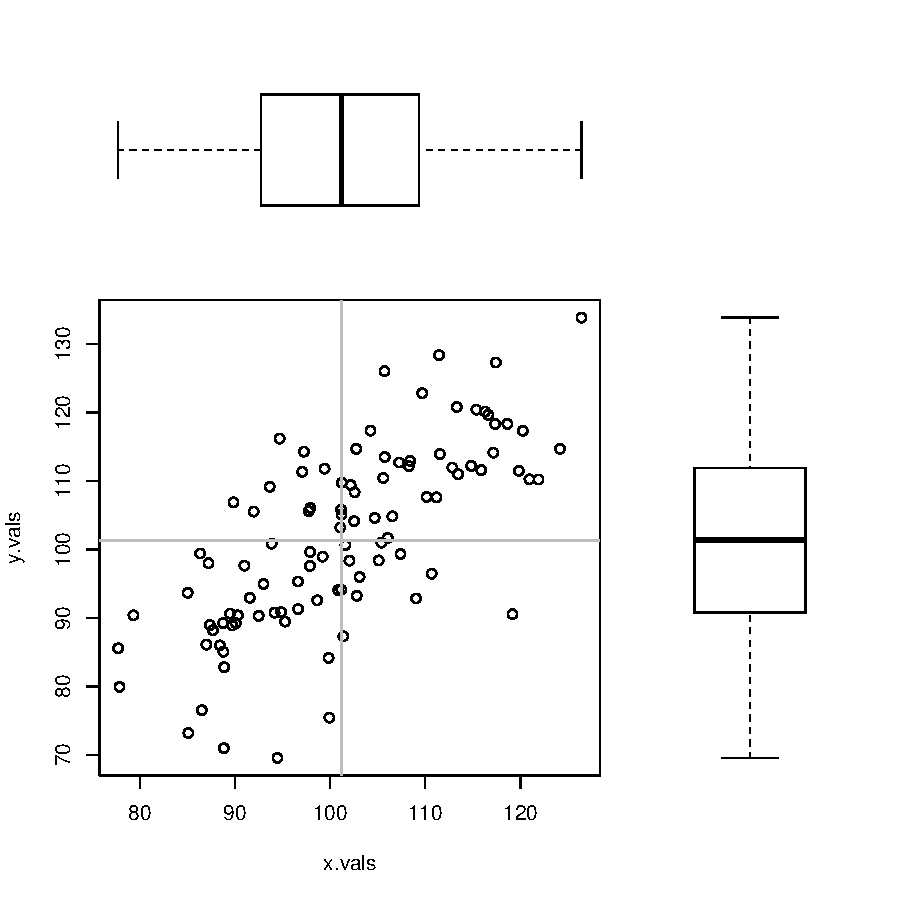
\includegraphics[width=\maxwidth]{figure/unnamed-chunk-182-1} 

\end{knitrout}
\end{footnotesize}


\section{Using alternative fonts in pdfs with the extrafont package}

If you don't like the default font that R uses in creating plots, you can use the \texttt{extrafont} package to use additional fonts in plots saved as .pdf files. However, let me warn you that it's not as easy as just selecting a font from a drop-down menu (like in Word). To use other fonts, follow these four steps:

First, install and load the \texttt{extrafont} package

\begin{knitrout}
\definecolor{shadecolor}{rgb}{0.969, 0.969, 0.969}\color{fgcolor}\begin{kframe}
\begin{alltt}
\hlkwd{install.packages}\hlstd{(}\hlstr{"extrafont"}\hlstd{)}
\hlkwd{library}\hlstd{(}\hlstr{"extrafont"}\hlstd{)}
\end{alltt}
\end{kframe}
\end{knitrout}

\begin{knitrout}
\definecolor{shadecolor}{rgb}{0.969, 0.969, 0.969}\color{fgcolor}\begin{kframe}


{\ttfamily\noindent\itshape\color{messagecolor}{\#\# Registering fonts with R}}\end{kframe}
\end{knitrout}


Second, import the fonts on your computer into R by running the \texttt{font\_import()} function. When you execute this, you'll receive a warning telling you that importing the fonts may take a few minutes. Type "y" and watch R do it's magic. Don't worry if you see some warnings or if it takes a few minutes,once you've run \texttt{font\_import()} once you \textit{won't} need to run it again on your machine.

\begin{knitrout}
\definecolor{shadecolor}{rgb}{0.969, 0.969, 0.969}\color{fgcolor}\begin{kframe}
\begin{alltt}
\hlkwd{font_import}\hlstd{()}
\end{alltt}
\end{kframe}
\end{knitrout}

Third,load your fonts into your current R session using the function \texttt{loadfonts()}. Unfortunately, you DO need to run this in each R session.

\begin{knitrout}
\definecolor{shadecolor}{rgb}{0.969, 0.969, 0.969}\color{fgcolor}\begin{kframe}
\begin{alltt}
\hlkwd{loadfonts}\hlstd{()}
\end{alltt}
\end{kframe}
\end{knitrout}


Now you're ready to go. To see which fonts are available to use in your plots, use the \texttt{fonts()} function. When you execute this function, you'll see a table with all the fonts you can use. Let's do this on my system (I'll just print the first 50 values here)

\begin{tiny}
\begin{knitrout}
\definecolor{shadecolor}{rgb}{0.969, 0.969, 0.969}\color{fgcolor}\begin{kframe}
\begin{alltt}
\hlkwd{fonts}\hlstd{()[}\hlnum{1}\hlopt{:}\hlnum{50}\hlstd{]} \hlcom{# Show me the first 50 fonts on my system}
\end{alltt}
\begin{verbatim}
##  [1] ".Keyboard"                       "Andale Mono"                    
##  [3] "Apple Braille"                   "AppleMyungjo"                   
##  [5] "Arial Black"                     "Arial"                          
##  [7] "Arial Narrow"                    "Arial Rounded MT Bold"          
##  [9] "Arial Unicode MS"                "Brush Script MT"                
## [11] "Comic Sans MS"                   "Courier New"                    
## [13] "DIN Alternate"                   "DIN Condensed"                  
## [15] "Georgia"                         "Impact"                         
## [17] "Khmer Sangam MN"                 "Lao Sangam MN"                  
## [19] "Microsoft Sans Serif"            "Myanmar Sangam MN"              
## [21] "Tahoma"                          "Times New Roman"                
## [23] "Trebuchet MS"                    "Verdana"                        
## [25] "Webdings"                        "Wingdings"                      
## [27] "Wingdings 2"                     "Wingdings 3"                    
## [29] "Helvetica LT Std  steevo harvie" "Helvetica World"                
## [31] "HelvFB"                          "HelvFE"                         
## [33] "Helvetica-Black-SemiBold"        "Helvetica"                      
## [35] "Helvetica-Condensed-Black-Se"    "Helvetica-Condensed-Light-Li"   
## [37] "Helvetica-Condensed-Light-Light" "Helvetica-Condensed-Thin"       
## [39] "Helvetica-Conth"                 "Helvetica-Light-Light-Italic"   
## [41] "Helvetica-Normal"                "HelveticaExt-No"                
## [43] "HelveticaExtO 2"                 "HelveticaExtO 3"                
## [45] "HelveticaExtO 4"                 "HelveticaInserat-Roman-SemiB"   
## [47] "HelveticaInserat-Roman-SemiBold" "HelveticaNeueLT Com 55 Roman"   
## [49] "HelveticaNeueLT Com 57 Cn"       "HelveticaNeueLT Com 53 Ex"
\end{verbatim}
\end{kframe}
\end{knitrout}
\end{tiny}

You will likely have more or less fonts than I have on my system - if you want more fonts, you'll need to download them. Now that we have a list of fonts we can use, we can finally create a plot using the new font. To do this, we need to add two special arguments when creating our plot:

\begin{enumerate}
\item In the \texttt{pdf()} function, add the argument \texttt{family = "fontname"}, where \texttt{fontname} is the name of the font you want to use.
\item After executing \texttt{dev.off()} to finish the plot, execute the command \texttt{embed\_fonts("filename.pdf")}. This command will embed the font in the pdf file.
\end{enumerate}

Let's follow these steps to create a plot using the Helvetica Light font. Again, I found this font on my computer by running \texttt{fonts()}. If you don't have this font on your computer, then it won't work for you. Instead, replace the argument \texttt{"HelvLight"} with a different font on your system:


\begin{knitrout}
\definecolor{shadecolor}{rgb}{0.969, 0.969, 0.969}\color{fgcolor}\begin{kframe}
\begin{alltt}
\hlkwd{pdf}\hlstd{(}\hlstr{"/Users/Nathaniel/Dropbox/Git/YaRrr_Book/media/helveticalight.pdf"}\hlstd{,}
    \hlkwc{width} \hlstd{=} \hlnum{4}\hlstd{,} \hlkwc{height} \hlstd{=} \hlnum{4}\hlstd{,}
    \hlkwc{family} \hlstd{=} \hlstr{"HelvLight"} \hlcom{# Specify the font in the plot}
    \hlstd{)}

\hlkwd{hist}\hlstd{(}\hlkwc{x} \hlstd{=} \hlkwd{rnorm}\hlstd{(}\hlnum{100}\hlstd{),} \hlcom{# some random data}
     \hlkwc{col} \hlstd{=} \hlstr{"skyblue"}\hlstd{,}
     \hlkwc{main} \hlstd{=} \hlstr{"Helvetica Light font"}\hlstd{)}

\hlkwd{dev.off}\hlstd{()}
\end{alltt}
\begin{verbatim}
## pdf 
##   2
\end{verbatim}
\begin{alltt}
\hlkwd{embed_fonts}\hlstd{(}\hlstr{"/Users/Nathaniel/Dropbox/Git/YaRrr_Book/media/helveticalight.pdf"}\hlstd{)} \hlcom{# Embed the fonts in the pdf}
\end{alltt}
\end{kframe}
\end{knitrout}

Look at Figure X to see the plot that this code created

\begin{marginfigure}
\includegraphics[]{/Users/Nathaniel/Dropbox/Git/YaRrr_Book/media/helveticalight.pdf}
\caption{Plot created with Helvetica Light font (see the main text for plotting code).}
\label{fig:helvetica}
\end{marginfigure}


\pagebreak
\section{Additional Tips}

\begin{itemize}


  \item To change the background color of a plot, add the command \texttt{par(bg = mycolor)} (where \textt{my.color} is the color you want to use) prior to creating the plot. For example, the following code will put a light gray background behind a histogram:
  
\begin{knitrout}
\definecolor{shadecolor}{rgb}{0.969, 0.969, 0.969}\color{fgcolor}\begin{kframe}
\begin{alltt}
\hlkwd{par}\hlstd{(}\hlkwc{bg} \hlstd{=} \hlkwd{gray}\hlstd{(}\hlnum{.9}\hlstd{))}
\hlkwd{hist}\hlstd{(}\hlkwc{x} \hlstd{=} \hlkwd{rnorm}\hlstd{(}\hlnum{100}\hlstd{))}
\end{alltt}
\end{kframe}
\includegraphics[width=\maxwidth]{figure/unnamed-chunk-189-1} 

\end{knitrout}

See Figure~\ref{fig:coloredbackground} for a nicer example.

\begin{marginfigure}
\begin{tiny}
\begin{knitrout}
\definecolor{shadecolor}{rgb}{0.969, 0.969, 0.969}\color{fgcolor}\begin{kframe}
\begin{alltt}
\hlkwd{pdf}\hlstd{(}\hlstr{"/Users/Nathaniel/Dropbox/Git/YaRrr_Book/media/parrothelvetica.pdf"}\hlstd{,}
    \hlkwc{width} \hlstd{=} \hlnum{8}\hlstd{,} \hlkwc{height} \hlstd{=} \hlnum{6}\hlstd{,} \hlkwc{family} \hlstd{=} \hlstr{"HelvLight"}\hlstd{)}

\hlstd{parrot.data} \hlkwb{<-} \hlkwd{data.frame}\hlstd{(}
  \hlstr{"parrots"} \hlstd{=} \hlnum{0}\hlopt{:}\hlnum{6}\hlstd{,}
  \hlstr{"female"} \hlstd{=} \hlkwd{c}\hlstd{(}\hlnum{200}\hlstd{,} \hlnum{150}\hlstd{,} \hlnum{100}\hlstd{,} \hlnum{175}\hlstd{,} \hlnum{55}\hlstd{,} \hlnum{25}\hlstd{,} \hlnum{10}\hlstd{),}
  \hlstr{"male"} \hlstd{=} \hlkwd{c}\hlstd{(}\hlnum{150}\hlstd{,} \hlnum{125}\hlstd{,} \hlnum{180}\hlstd{,} \hlnum{242}\hlstd{,} \hlnum{10}\hlstd{,} \hlnum{62}\hlstd{,} \hlnum{5}\hlstd{)}
  \hlstd{)}

\hlstd{n.data} \hlkwb{<-} \hlkwd{nrow}\hlstd{(parrot.data)}

\hlkwd{par}\hlstd{(}\hlkwc{bg} \hlstd{=} \hlkwd{rgb}\hlstd{(}\hlnum{61}\hlstd{,} \hlnum{55}\hlstd{,} \hlnum{72}\hlstd{,} \hlkwc{maxColorValue} \hlstd{=} \hlnum{255}\hlstd{),}
    \hlkwc{mar} \hlstd{=} \hlkwd{c}\hlstd{(}\hlnum{8}\hlstd{,} \hlnum{6}\hlstd{,} \hlnum{6}\hlstd{,} \hlnum{3}\hlstd{)}
    \hlstd{)}

\hlkwd{plot}\hlstd{(}\hlnum{1}\hlstd{,} \hlkwc{xlab} \hlstd{=} \hlstr{""}\hlstd{,} \hlkwc{ylab} \hlstd{=} \hlstr{""}\hlstd{,} \hlkwc{xaxt} \hlstd{=} \hlstr{"n"}\hlstd{,}
     \hlkwc{yaxt} \hlstd{=} \hlstr{"n"}\hlstd{,} \hlkwc{main} \hlstd{=} \hlstr{""}\hlstd{,} \hlkwc{bty} \hlstd{=} \hlstr{"n"}\hlstd{,} \hlkwc{type} \hlstd{=} \hlstr{"n"}\hlstd{,}
     \hlkwc{ylim} \hlstd{=} \hlkwd{c}\hlstd{(}\hlnum{0}\hlstd{,} \hlnum{250}\hlstd{),} \hlkwc{xlim} \hlstd{=} \hlkwd{c}\hlstd{(}\hlnum{.5}\hlstd{, n.data} \hlopt{+} \hlnum{.5}\hlstd{)}
     \hlstd{)}

\hlkwd{abline}\hlstd{(}\hlkwc{h} \hlstd{=} \hlkwd{seq}\hlstd{(}\hlnum{0}\hlstd{,} \hlnum{250}\hlstd{,} \hlnum{50}\hlstd{),} \hlkwc{lty} \hlstd{=} \hlnum{3}\hlstd{,} \hlkwc{col} \hlstd{=} \hlkwd{gray}\hlstd{(}\hlnum{.95}\hlstd{),} \hlkwc{lwd} \hlstd{=} \hlnum{1}\hlstd{)}

\hlkwd{mtext}\hlstd{(}\hlkwc{text} \hlstd{=} \hlkwd{seq}\hlstd{(}\hlnum{50}\hlstd{,} \hlnum{250}\hlstd{,} \hlnum{50}\hlstd{),}
      \hlkwc{side} \hlstd{=} \hlnum{2}\hlstd{,} \hlkwc{at} \hlstd{=} \hlkwd{seq}\hlstd{(}\hlnum{50}\hlstd{,} \hlnum{250}\hlstd{,} \hlnum{50}\hlstd{),}
      \hlkwc{las} \hlstd{=} \hlnum{1}\hlstd{,} \hlkwc{line} \hlstd{=} \hlnum{1}\hlstd{,} \hlkwc{col} \hlstd{=} \hlkwd{gray}\hlstd{(}\hlnum{.95}\hlstd{))}

\hlkwd{mtext}\hlstd{(}\hlkwc{text} \hlstd{=} \hlkwd{paste}\hlstd{(}\hlnum{0}\hlopt{:}\hlstd{(n.data} \hlopt{-} \hlnum{1}\hlstd{),} \hlstr{" Parrots"}\hlstd{),}
      \hlkwc{side} \hlstd{=} \hlnum{1}\hlstd{,} \hlkwc{at} \hlstd{=} \hlnum{1}\hlopt{:}\hlstd{n.data,} \hlkwc{las} \hlstd{=} \hlnum{1}\hlstd{,}
      \hlkwc{line} \hlstd{=} \hlnum{1}\hlstd{,} \hlkwc{col} \hlstd{=} \hlkwd{gray}\hlstd{(}\hlnum{.95}\hlstd{))}


\hlstd{female.col} \hlkwb{<-} \hlkwd{gray}\hlstd{(}\hlnum{1}\hlstd{,} \hlkwc{alpha} \hlstd{=} \hlnum{.7}\hlstd{)}
\hlstd{male.col} \hlkwb{<-} \hlkwd{rgb} \hlstd{(}\hlnum{226}\hlstd{,} \hlnum{89}\hlstd{,} \hlnum{92}\hlstd{,} \hlkwc{maxColorValue} \hlstd{=} \hlnum{255}\hlstd{,} \hlkwc{alpha} \hlstd{=} \hlnum{220}\hlstd{)}

\hlstd{rect.width} \hlkwb{<-} \hlnum{.35}
\hlstd{rect.space} \hlkwb{<-} \hlnum{.04}

\hlkwd{rect}\hlstd{(}\hlnum{1}\hlopt{:}\hlstd{n.data} \hlopt{-} \hlstd{rect.width} \hlopt{-} \hlstd{rect.space} \hlopt{/} \hlnum{2}\hlstd{,}
     \hlkwd{rep}\hlstd{(}\hlnum{0}\hlstd{, n.data),}
     \hlnum{1}\hlopt{:}\hlstd{n.data} \hlopt{-} \hlstd{rect.space} \hlopt{/} \hlnum{2}\hlstd{,}
     \hlstd{parrot.data}\hlopt{$}\hlstd{female,}
     \hlkwc{col} \hlstd{= female.col,} \hlkwc{border} \hlstd{=} \hlnum{NA}
     \hlstd{)}

\hlkwd{rect}\hlstd{(}\hlnum{1}\hlopt{:}\hlstd{n.data} \hlopt{+} \hlstd{rect.space} \hlopt{/} \hlnum{2}\hlstd{,}
     \hlkwd{rep}\hlstd{(}\hlnum{0}\hlstd{, n.data),}
     \hlnum{1}\hlopt{:}\hlstd{n.data} \hlopt{+} \hlstd{rect.width} \hlopt{+} \hlstd{rect.space} \hlopt{/} \hlnum{2}\hlstd{,}
     \hlstd{parrot.data}\hlopt{$}\hlstd{male,}
     \hlkwc{col} \hlstd{= male.col,} \hlkwc{border} \hlstd{=} \hlnum{NA}
     \hlstd{)}

\hlkwd{legend}\hlstd{(n.data} \hlopt{-} \hlnum{1}\hlstd{,} \hlnum{250}\hlstd{,} \hlkwd{c}\hlstd{(}\hlstr{"Male Pirates"}\hlstd{,} \hlstr{"Female Pirates"}\hlstd{),}
       \hlkwc{col} \hlstd{=} \hlkwd{c}\hlstd{(female.col, male.col),} \hlkwc{pch} \hlstd{=} \hlkwd{rep}\hlstd{(}\hlnum{15}\hlstd{,} \hlnum{2}\hlstd{),}
       \hlkwc{bty} \hlstd{=} \hlstr{"n"}\hlstd{,} \hlkwc{pt.cex} \hlstd{=} \hlnum{1.5}\hlstd{,} \hlkwc{text.col} \hlstd{=} \hlstr{"white"}
       \hlstd{)}

\hlkwd{mtext}\hlstd{(}\hlstr{"Number of parrots owned by pirates"}\hlstd{,} \hlkwc{side} \hlstd{=} \hlnum{3}\hlstd{,}
      \hlkwc{at} \hlstd{= n.data} \hlopt{+} \hlnum{.5}\hlstd{,} \hlkwc{adj} \hlstd{=} \hlnum{1}\hlstd{,} \hlkwc{cex} \hlstd{=} \hlnum{1.2}\hlstd{,} \hlkwc{col} \hlstd{=} \hlstr{"white"}\hlstd{)}

\hlkwd{mtext}\hlstd{(}\hlstr{"Source: Drunken survey on 22 May 2015"}\hlstd{,} \hlkwc{side} \hlstd{=} \hlnum{1}\hlstd{,}
      \hlkwc{at} \hlstd{=} \hlnum{0}\hlstd{,} \hlkwc{adj} \hlstd{=} \hlnum{0}\hlstd{,} \hlkwc{line} \hlstd{=} \hlnum{3}\hlstd{,} \hlkwc{font} \hlstd{=} \hlnum{3}\hlstd{,} \hlkwc{col} \hlstd{=} \hlstr{"white"}\hlstd{)}

\hlkwd{dev.off}\hlstd{()}
\end{alltt}
\begin{verbatim}
## pdf 
##   2
\end{verbatim}
\begin{alltt}
\hlkwd{embed_fonts}\hlstd{(}\hlstr{"/Users/Nathaniel/Dropbox/Git/YaRrr_Book/media/parrothelvetica.pdf"}\hlstd{)} \hlcom{# Embed the fonts in the pdf}
\end{alltt}
\end{kframe}
\end{knitrout}
\end{tiny}
\includegraphics[]{/Users/Nathaniel/Dropbox/Git/YaRrr_Book/media/parrothelvetica.pdf}
\caption{Use \texttt{par(bg = my.color)} before creating a plot to add a colored background. The design of this plot was inspired by \texttt{http://www.vox.com/2015/5/20/8625785/expensive-wine-taste-cheap}.}
\label{fig:coloredbackground}
\end{marginfigure}


\item Sometimes you'll mess so much with plotting parameters that you may want to set things back to their default value. To see the default values for all the plotting parameters, execute the code \texttt{par()} to print the default parameter values for all plotting parameters to the console.



\end{itemize}


%----------------------------------------------------------------------------------------
%	CHAPTER 9
%----------------------------------------------------------------------------------------

\chapter{9: Advanced dataframe manipulation}
\label{ch:9}


Chapter Goals

\begin{enumerate}
  \item Grouped aggregation with aggregate() and dplyr
  \item Merging datasets with merge()
  \item Common data management tasks: rescaling, recoding
\end{enumerate}


In this chapter, we'll cover how to do advanced dataframe manipulation. You'll learn how to recode values of a dataframe and quickly and easily calculate summary data from a dataframe, 


\section{Recoding values in a vector}

%' 
%' 
%' \begin{marginfigure}
%' \begin{tiny}
%' <<>>=
%' # Create blank plot with no margins
%' par(mar = rep(0, 4))
%' plot(1, xlim = c(0, 1), ylim = c(0, 13), 
%'      bty = "n", xlab = "", ylab = "", main = "",
%'      type = "n", xaxt = "n", yaxt = "n")
%' 
%' data.vec <- c(-3, 0, 5)
%' 
%' # Original
%' text(.5, 12.5, "Original", cex = 2)
%' 
%' text(rep(.5, 3), 9:11, data.vec)
%' rect(.45, 8.5, .55, 11.5)
%' 
%' # Step 1
%' left <- .2
%' 
%' text(left, 7.5, "Step 1 - Copy", cex = 1.5)
%' text(left, 6.5, "new <- old", cex = 1)
%' 
%' 
%' text(rep(left, 3), 3:5, data.vec)
%' rect(left - .05, 2.5, left + .05, 5.5)
%' 
%' # Step 2
%' mid <- .5
%' 
%' text(mid, 7.5, "Step 2 - Index", cex = 1.5)
%' text(mid, 6.5, "log.vec <- condition", cex = 1)
%' 
%' 
%' text(rep(mid - .1, 3), 3:5, data.vec)
%' rect(mid - .15, 2.5, mid - .05, 5.5)
%' 
%' text(rep(mid - .03, 3), 3:5, rep("< 0", 3))
%' 
%' text(rep(mid + .05, 3), 3:5, data.vec < 0)
%' rect(mid, 2.5, mid + .1, 5.5)
%' 
%' # Step 3
%' right <- .75
%' 
%' text(right, 7.5, "Step 3 - Assign", cex = 1.5)
%' text(right, 6.5, "new[log.vec] <- value", cex = 1)
%' 
%' 
%' @
%' \end{tiny}
%' \label{fig:recoding}
%' \caption{A visual representation of how indexing with logical vectors works in R. When you apply a logical vector (a vector containing only TRUE and FALSE values) to a data vector, R will return the the values in the data vector where the logical vector is TRUE.}
%' \end{marginfigure}
%' @


Let's say that you conducted an online survey where you asked 100 people some basic demographic information and then asked them how happy they are with their life on a scale from 1 to 8. When you look at the dataset, you realize that many people gave invalid answers to the questions. For example, some people said they had a negative income and had a negative number of siblings. How can you fix these data? In this chapter, we'll cover the basics of data-recoding

There are three basic steps to recoding values in a vector:

\marginnote{

\textbf{3 Steps to recoding values}

\begin{enumerate}
\item Copy the original column (\texttt{original}) to a new column with a new name (\texttt{new}) using assignment.
\item Create a logical vector indicating which values of \texttt{new} should be converted.
\item Index \texttt{new} by the logical vector and assign the updated value to it.
\end{enumerate}

}

\subsection{3 Steps to recoding values}

\begin{enumerate}

\item Copy the original column (\texttt{original}) to a new column with a new name (\texttt{new}) using assignment.
\item Create a logical vector indicating which values of \texttt{new} should be converted.
\item Index \texttt{new} by the logical vector and assign the updated value to it.

\end{enumerate}

Let's start with a dummy example where we take the integers from 1 to 10, then convert all values greater than 5 to 999

\begin{knitrout}
\definecolor{shadecolor}{rgb}{0.969, 0.969, 0.969}\color{fgcolor}\begin{kframe}
\begin{alltt}
\hlstd{original} \hlkwb{<-} \hlnum{1}\hlopt{:}\hlnum{10}

\hlstd{new.vec} \hlkwb{<-} \hlstd{original} \hlcom{# Step 1}
\hlstd{log.vec} \hlkwb{<-} \hlstd{new.vec} \hlopt{>} \hlnum{5} \hlcom{# Step 2}
\hlstd{new.vec[log.vec]} \hlkwb{<-} \hlnum{999} \hlcom{# Step 3}

\hlstd{new.vec}
\end{alltt}
\begin{verbatim}
##  [1]   1   2   3   4   5 999 999 999 999 999
\end{verbatim}
\end{kframe}
\end{knitrout}

As you can see, our new vector \texttt{new.vec} is identical to the integers 1 to 10 up until the value of 6, where all values have been converted to 999.

\subsection{Recoding values from the pirate survey}
 
Let's start by using the dataset \texttt{pirate\_survey\_werrors.txt} which is stored at http://nathanieldphillips.com/wp-content/uploads/2015/05/pirate\_survey\_werrors.txt. This is a tab-delimited file containing results from 1,000 pirates.

To load the data, execute the following commands:

\begin{knitrout}
\definecolor{shadecolor}{rgb}{0.969, 0.969, 0.969}\color{fgcolor}\begin{kframe}
\begin{alltt}
\hlstd{pirates.errors} \hlkwb{<-} \hlkwd{read.table}\hlstd{(}\hlstr{"http://nathanieldphillips.com/wp-content/uploads/2015/05/pirate_survey_werrors.txt"}\hlstd{,} \hlkwc{sep} \hlstd{=} \hlstr{"\textbackslash{}t"}\hlstd{,} \hlkwc{stringsAsFactors} \hlstd{= F)}
\end{alltt}
\end{kframe}
\end{knitrout}


Unfortunately, some pirates decided to supply some invalid answers. We'll start with the \texttt{sex} variable. To see the values that are currently in this column, we'll run \texttt{table()}:

\begin{knitrout}
\definecolor{shadecolor}{rgb}{0.969, 0.969, 0.969}\color{fgcolor}\begin{kframe}
\begin{alltt}
\hlkwd{table}\hlstd{(pirates.errors}\hlopt{$}\hlstd{sex)}
\end{alltt}
\begin{verbatim}
## 
## depends on who is offering                     female 
##                          3                        477 
##                       male                   other/NA 
##                        474                         44 
##        sure I'll have some 
##                          2
\end{verbatim}
\end{kframe}
\end{knitrout}

Very funny guys. There should only be three valid responses to this question: female, male, and other/NA. Let's recode all the other values to NA. We'll do this in three steps:

\begin{enumerate}

  \item Copy the values of \texttt{sex} into a new vector called \texttt{sex.r} standing for "sex recoded"
  \item Create a logical vector called \texttt{log.vec} that indicates which values of sex.r are valid - that is, in the set of values \texttt{c("female", "male", "other/NA")}
  \item Assign a value of \texttt{NA} to all values of \texttt{sex.r} for which \texttt{log.vec} is FALSE.
  
\end{enumerate}



\begin{knitrout}
\definecolor{shadecolor}{rgb}{0.969, 0.969, 0.969}\color{fgcolor}\begin{kframe}
\begin{alltt}
\hlcom{# Step 1: Copy sex to a new column called sex.r }
\hlstd{pirates.errors}\hlopt{$}\hlstd{sex.r} \hlkwb{<-} \hlstd{pirates.errors}\hlopt{$}\hlstd{sex}

\hlcom{# Step 2: Create a logical vector indicating which values are valid}
\hlstd{log.vec} \hlkwb{<-} \hlstd{pirates.errors}\hlopt{$}\hlstd{sex.r} \hlopt \hlkwd{c}\hlstd{(}\hlstr{"female"}\hlstd{,} \hlstr{"male"}\hlstd{,} \hlstr{"other/NA"}\hlstd{)}

\hlcom{# Step 3: Recode all invalid values to NA}
\hlstd{pirates.errors}\hlopt{$}\hlstd{sex.r[log.vec} \hlopt{==} \hlnum{FALSE}\hlstd{]} \hlkwb{<-} \hlnum{NA} \hlcom{# Step 3}
\end{alltt}
\end{kframe}
\end{knitrout}


Let's make sure this worked by looking at the values of \texttt{sex.r}. Hopefully, we will only see valid entries now:

\begin{footnotesize}
\begin{knitrout}
\definecolor{shadecolor}{rgb}{0.969, 0.969, 0.969}\color{fgcolor}\begin{kframe}
\begin{alltt}
\hlkwd{table}\hlstd{(pirates.errors}\hlopt{$}\hlstd{sex.r,} \hlkwc{useNA} \hlstd{=} \hlstr{"ifany"}\hlstd{)}
\end{alltt}
\begin{verbatim}
## 
##   female     male other/NA     <NA> 
##      477      474       44        5
\end{verbatim}
\end{kframe}
\end{knitrout}
\end{footnotesize}

As you can see, our new column \texttt{sex.r} only contains valid entries, so it looks like our recoding did what we wanted. \marginnote{Note that the \texttt{table()} function does not (by default), show NA values. To see how many NA values are in the dataset, you can include the argument \texttt{useNA = "ifany"} as in \texttt{table(pirates.errors\$sex.r, useNA = "ifany")}}

Let's do the same with \texttt{age} and \texttt{tattoos}. The column \texttt{age} should be an integer between 18 and 99, and the values of \texttt{tattoos} should be an integer between 0 and a maximum of (let's say) 100. Let's start by looking at the current values of each column using the \texttt{table()} function:

\begin{footnotesize}
\begin{knitrout}
\definecolor{shadecolor}{rgb}{0.969, 0.969, 0.969}\color{fgcolor}\begin{kframe}
\begin{alltt}
\hlkwd{table}\hlstd{(pirates.errors}\hlopt{$}\hlstd{age)}
\end{alltt}
\begin{verbatim}
## 
##   -99     0    12    13    14    15    16    17    18    19    20    21 
##     2     5     2     3     2     7    10    11    17    24    30    48 
##    22    23    24    25    26    27    28    29    30    31    32    33 
##    45    43    65    57    62    81    71    63    46    62    58    37 
##    34    35    36    37    38    39    40    41    42    44    49   500 
##    37    25    20    22    19     6     3     1     1     1     1     6 
##   999 12345 
##     4     3
\end{verbatim}
\begin{alltt}
\hlkwd{table}\hlstd{(pirates.errors}\hlopt{$}\hlstd{tattoos)}
\end{alltt}
\begin{verbatim}
## 
##   -10     0     1     2     3     4     5     6     7     8     9    10 
##     2    11     5    13    20    25    51    68    91   104   112   112 
##    11    12    13    14    15    16    17    18    19    20 1e+06 
##   119    80    58    45    37    22     8     4     4     1     5
\end{verbatim}
\end{kframe}
\end{knitrout}
\end{footnotesize}

We can see some problems here: \texttt{age} has some negative values and a few very large values. Further, \texttt{tattoos} has a few negative values and a few values greater than 100. Let's convert all these troublesome values of \texttt{age} to NA.

\begin{footnotesize}
\begin{knitrout}
\definecolor{shadecolor}{rgb}{0.969, 0.969, 0.969}\color{fgcolor}\begin{kframe}
\begin{alltt}
\hlcom{# Step 1: Copy age to a new column age.r}
\hlstd{pirates.errors}\hlopt{$}\hlstd{age.r} \hlkwb{<-} \hlstd{pirates.errors}\hlopt{$}\hlstd{age}

\hlcom{# Step 2: See which values of age.r are valid}
\hlstd{age.valid} \hlkwb{<-} \hlstd{pirates.errors}\hlopt{$}\hlstd{age.r} \hlopt{>=} \hlnum{18} \hlopt{&} \hlstd{pirates.errors}\hlopt{$}\hlstd{age.r} \hlopt{<=} \hlnum{99} \hlcom{# Step 2}

\hlcom{# Step 3: Recode non-valid values to NA}
\hlstd{pirates.errors}\hlopt{$}\hlstd{age.r[age.valid} \hlopt{==} \hlnum{FALSE}\hlstd{]} \hlkwb{<-} \hlnum{NA} \hlcom{# Step 3}
\end{alltt}
\end{kframe}
\end{knitrout}
\end{footnotesize}

Now let's do the same for tattoos:

\begin{knitrout}
\definecolor{shadecolor}{rgb}{0.969, 0.969, 0.969}\color{fgcolor}\begin{kframe}
\begin{alltt}
\hlcom{# Step 1: Copy tattoos to a new column tattoos.r}
\hlstd{pirates.errors}\hlopt{$}\hlstd{tattoos.r} \hlkwb{<-} \hlstd{pirates.errors}\hlopt{$}\hlstd{tattoos}

\hlcom{# Step 2: See which values of tattoos.r are valid}
\hlstd{tattoos.valid} \hlkwb{<-} \hlstd{pirates.errors}\hlopt{$}\hlstd{tattoos.r} \hlopt \hlnum{0}\hlopt{:}\hlnum{100} \hlcom{# Step 2}

\hlcom{# Step 3: Recode non-valid values to NA}
\hlstd{pirates.errors}\hlopt{$}\hlstd{tattoos.r[tattoos.valid} \hlopt{==} \hlnum{FALSE}\hlstd{]} \hlkwb{<-} \hlnum{NA} \hlcom{# Step 3}
\end{alltt}
\end{kframe}
\end{knitrout}



Now, let's look at the frequency tables of these recoded values:

\begin{footnotesize}
\begin{knitrout}
\definecolor{shadecolor}{rgb}{0.969, 0.969, 0.969}\color{fgcolor}\begin{kframe}
\begin{alltt}
\hlkwd{table}\hlstd{(pirates.errors}\hlopt{$}\hlstd{age.r,} \hlkwc{useNA} \hlstd{=} \hlstr{"always"}\hlstd{)}
\end{alltt}
\begin{verbatim}
## 
##   18   19   20   21   22   23   24   25   26   27   28   29   30   31   32 
##   17   24   30   48   45   43   65   57   62   81   71   63   46   62   58 
##   33   34   35   36   37   38   39   40   41   42   44   49 <NA> 
##   37   37   25   20   22   19    6    3    1    1    1    1   55
\end{verbatim}
\begin{alltt}
\hlkwd{table}\hlstd{(pirates.errors}\hlopt{$}\hlstd{tattoos.r,} \hlkwc{useNA} \hlstd{=} \hlstr{"always"}\hlstd{)}
\end{alltt}
\begin{verbatim}
## 
##    0    1    2    3    4    5    6    7    8    9   10   11   12   13   14 
##   11    5   13   20   25   51   68   91  104  112  112  119   80   58   45 
##   15   16   17   18   19   20 <NA> 
##   37   22    8    4    4    1   10
\end{verbatim}
\end{kframe}
\end{knitrout}
\end{footnotesize}

In these examples, we converted invalid values to NA. Of course, there's no reason why we couldn't recode the values to other values. For example, we might recode values of \texttt{tattoos} greater than 50 to the maximum possible value of 50. To do this, we can just change the assignment in Step 3 to a value of \texttt{50} instead of NA.


\section{Splitting numerical data into groups using cut()}

When we create some plots and analyses, we may want to group numerical data into bins of similar values. For example, in our pirate survey, we might want to group pirates into age decades, where all pirates in their 20s are in one group, all those in their 30s go into another group, etc. Once we have these bins, we can calculate aggreagte statistics for each group.

R has a handy function for grouping numerical data called \texttt{cut()}



\vspace{5mm} %5mm vertical space
\noindent
\setlength{\fboxrule}{1.5pt}
\fbox{
\parbox{\textwidth}{

\newfun{cut()}\index{cut()}

\hline

\begin{description}

  \item[\tt{x}] \hfill \\
     A vector of numeric data
        \item[\tt{breaks}] \hfill \\
  Either a numeric vector of two or more unique cut points or a single number (greater than or equal to 2) giving the number of intervals into which x is to be cut. For example, \texttt{breaks = 1:10} will put break points at all integers from 1 to 10, while \texttt{breaks = 5} will split the data into 5 equal sections.
         \item[\tt{labels}] \hfill \\
An optional string vector of labels for each grouping. By default, labels are constructed using "(a,b]" interval notation. If labels = FALSE, simple integer codes are returned instead of a factor.
        \item[\tt{right}] \hfill \\
 A logical value indicating if the intervals should be closed on the right (and open on the left) or vice versa.

\end{description}

}
}
\vspace{5mm} %5mm vertical space

Let's try a simple example by converting the integers from 1 to 50 into bins of size 10:

\begin{footnotesize}
\begin{knitrout}
\definecolor{shadecolor}{rgb}{0.969, 0.969, 0.969}\color{fgcolor}\begin{kframe}
\begin{alltt}
\hlkwd{cut}\hlstd{(}\hlnum{1}\hlopt{:}\hlnum{50}\hlstd{,} \hlkwd{seq}\hlstd{(}\hlnum{0}\hlstd{,} \hlnum{50}\hlstd{,} \hlnum{10}\hlstd{))}
\end{alltt}
\begin{verbatim}
##  [1] (0,10]  (0,10]  (0,10]  (0,10]  (0,10]  (0,10]  (0,10]  (0,10] 
##  [9] (0,10]  (0,10]  (10,20] (10,20] (10,20] (10,20] (10,20] (10,20]
## [17] (10,20] (10,20] (10,20] (10,20] (20,30] (20,30] (20,30] (20,30]
## [25] (20,30] (20,30] (20,30] (20,30] (20,30] (20,30] (30,40] (30,40]
## [33] (30,40] (30,40] (30,40] (30,40] (30,40] (30,40] (30,40] (30,40]
## [41] (40,50] (40,50] (40,50] (40,50] (40,50] (40,50] (40,50] (40,50]
## [49] (40,50] (40,50]
## Levels: (0,10] (10,20] (20,30] (30,40] (40,50]
\end{verbatim}
\end{kframe}
\end{knitrout}
\end{footnotesize}

As you can see, our result is a vector of factors, where the first ten elements are (0, 10], the next ten elements are (10, 20], and so on. In other words, the new vector treats all numbers from 1 to 10 as being the same, and all numbers from 11 to 20 as being the same.

Let's test the \texttt{cut()} function on the age data from \texttt{pirates}. We'll add a new column to the dataset called \texttt{age.binned}, which separates the age data into bins of size 10. This means that every pirate between the ages of 10 and 20 will be in the first bin, those between the ages of 21 and 30 will be in the second bin, and so on. To do this, we'll enter \texttt{pirates\$age} as the x argument, and \texttt{seq(10, 100, 10)} as the \texttt{breaks} argument:

\begin{footnotesize}
\begin{knitrout}
\definecolor{shadecolor}{rgb}{0.969, 0.969, 0.969}\color{fgcolor}\begin{kframe}
\begin{alltt}
\hlstd{pirates}\hlopt{$}\hlstd{age.cut} \hlkwb{<-} \hlkwd{cut}\hlstd{(}\hlkwc{x} \hlstd{= pirates}\hlopt{$}\hlstd{age,}  \hlcom{# The raw data}
                       \hlkwc{breaks} \hlstd{=} \hlkwd{seq}\hlstd{(}\hlnum{10}\hlstd{,} \hlnum{100}\hlstd{,} \hlnum{10}\hlstd{)}  \hlcom{# The break points of the cuts}
                       \hlstd{)}
\end{alltt}
\end{kframe}
\end{knitrout}
\end{footnotesize}

To show you how this worked, let's look at the first few rows of the columns \texttt{age} and \texttt{age.cut}

\begin{knitrout}
\definecolor{shadecolor}{rgb}{0.969, 0.969, 0.969}\color{fgcolor}\begin{kframe}
\begin{alltt}
\hlkwd{head}\hlstd{(pirates[}\hlkwd{c}\hlstd{(}\hlstr{"age"}\hlstd{,} \hlstr{"age.cut"}\hlstd{)])}
\end{alltt}
\begin{verbatim}
##   age age.cut
## 1  23 (20,30]
## 2  28 (20,30]
## 3  35 (30,40]
## 4  34 (30,40]
## 5  25 (20,30]
## 6  36 (30,40]
\end{verbatim}
\end{kframe}
\end{knitrout}

As you can see, \texttt{age.cut} has correctly converted the original age variable to a factor.

From these data, we can now easily calculate how many pirates are in each age group using \texttt{table()}

\begin{knitrout}
\definecolor{shadecolor}{rgb}{0.969, 0.969, 0.969}\color{fgcolor}\begin{kframe}
\begin{alltt}
\hlkwd{table}\hlstd{(pirates}\hlopt{$}\hlstd{age.cut)}
\end{alltt}
\begin{verbatim}
## 
##  (10,20]  (20,30]  (30,40]  (40,50]  (50,60]  (60,70]  (70,80]  (80,90] 
##      111      569      294        5        0        0        0        0 
## (90,100] 
##        0
\end{verbatim}
\end{kframe}
\end{knitrout}


\section{Grouped aggregation}

As you can see, we have quite a bit of data in our Flights dataset. Many of the questions we might want to answer with this dataset have to do with comparisons between groups. For example, ``What is the flight cancellation rate for each carrier?" or "What is the arrival delay for each destination?" In each of these questions, we want to know a descriptive statistic of a numeric variable (cancellation rate and arrival delay) as a function of a nominal independent variable (carrier and destination). By now, your R skills are good enough that you \textit{could} answer these questions already. You could do this by using \texttt{subset()} or logical indexing to slice and dice the data set for each level of the independent variable. However, it would be a pain to have to manually create new subsets or indexes for each level of the independent variable. Thankfully, R contains many functions that will help you do this in a snap.

The first function we'll cover is \texttt{aggregate()}. The function \texttt{aggregate()} takes three arguments, a formula in the form  \texttt{y {\raise.17ex\hbox{$\scriptstyle\sim$}} x1 + x2} defining the dependent (Y) and one or more independent variables (x1, x2, ...), a function (FUN), and a dataframe (data). When you execute \texttt{aggregate(\texttt{y {\raise.17ex\hbox{$\scriptstyle\sim$}} x1 + x2 + ...}, data, FUN)}, R will apply the input function (FUN) to the dependent variable (Y) \textit{separately} for each level(s) of the independent variable(s) (x1, x2, ...). Let's see how it works:




\vspace{5mm} %5mm vertical space
\noindent
\setlength{\fboxrule}{1.5pt}
\fbox{
\parbox{\textwidth}{

\newfun{aggregate()}\index{aggregate()}

\hline

\begin{description}

  \item[\tt{formula}] \hfill \\
     A formula in the form \texttt{y {\raise.17ex\hbox{$\scriptstyle\sim$}} x1 + x2 + ...} where y is the dependent variable, and x1, x2... are the index (independent) variables. For example, \texttt{salary {\raise.17ex\hbox{$\scriptstyle\sim$}} sex + age} will aggregate a \texttt{salary} column at every unique combination of \texttt{age} and \texttt{age}
        \item[\tt{FUN}] \hfill \\
   A function that you want to apply to x at every level of the independent variables. For example, \texttt{FUN = mean} will calculate the mean of the data
         \item[\tt{data}] \hfill \\
The dataset containing the variables in \texttt{formula}
        \item[\tt{...}] \hfill \\
Optional arguments passed on to FUN (like \tt{na.rm = T} to ignore NA values in x)

\end{description}

}
}
\vspace{5mm} %5mm vertical space


Let's give \texttt{aggregate()} a whirl. We'll use the function to answer the question ``What is the flight cancellation rate for each carrier?" For this question, we'll set the value of Y to \texttt{cancelled}, x1 to \texttt{carrier}, and FUN to \texttt{mean}

\begin{footnotesize}
\begin{knitrout}
\definecolor{shadecolor}{rgb}{0.969, 0.969, 0.969}\color{fgcolor}\begin{kframe}
\begin{alltt}
\hlkwd{aggregate}\hlstd{(}\hlkwc{formula} \hlstd{= cancelled} \hlopt{~} \hlstd{carrier,}  \hlcom{# DV is cancelled, IV is carrier}
          \hlkwc{FUN} \hlstd{= mean,} \hlcom{# Calculate the mean of the DV for each IV level}
          \hlkwc{na.rm} \hlstd{= T,} \hlcom{# Ignore NA values when calculating the mean}
          \hlkwc{data} \hlstd{= Flights} \hlcom{# IV and DV are located in the Flights dataframe}
          \hlstd{)}
\end{alltt}
\begin{verbatim}
##    carrier   cancelled
## 1       AA 0.018495684
## 2       AS 0.000000000
## 3       B6 0.025899281
## 4       CO 0.006782614
## 5       DL 0.015903067
## 6       EV 0.034482759
## 7       F9 0.007159905
## 8       FL 0.009817672
## 9       MQ 0.029044750
## 10      OO 0.013946828
## 11      UA 0.016409266
## 12      US 0.011268986
## 13      WN 0.015504047
## 14      XE 0.015495599
## 15      YV 0.012658228
\end{verbatim}
\end{kframe}
\end{knitrout}
\end{footnotesize}


As you can see, the \texttt{aggregate()} function has returned a dataframe with a column for the independent variable (\texttt{carrier}), and a column for the results of the function \texttt{mean} applied to each level of the independent variable. We can easily plot these data using the \texttt{barplot()} function, which plots a numeric variable as a function of a nominal variable (see margin Figure~\ref{fig:barplot})

\begin{marginfigure}
\begin{tiny}
\begin{knitrout}
\definecolor{shadecolor}{rgb}{0.969, 0.969, 0.969}\color{fgcolor}\begin{kframe}
\begin{alltt}
\hlstd{aggregated.data} \hlkwb{<-} \hlkwd{aggregate}\hlstd{(}\hlkwc{formula} \hlstd{= cancelled} \hlopt{~} \hlstd{carrier,}
                             \hlkwc{FUN} \hlstd{= mean,} \hlkwc{na.rm} \hlstd{= T,} \hlkwc{data} \hlstd{= Flights)}

\hlkwd{barplot}\hlstd{(}\hlkwc{height} \hlstd{= aggregated.data}\hlopt{$}\hlstd{cancelled,}
        \hlkwc{names.arg} \hlstd{= aggregated.data}\hlopt{$}\hlstd{carrier)}
\end{alltt}
\end{kframe}
\includegraphics[width=\maxwidth]{figure/unnamed-chunk-205-1} 

\end{knitrout}
\end{tiny}
\caption{Barplot showing the mean flight cancellation rate for airlines in the \texttt{Flights.txt} dataset}
\label{fig:barplot}
\end{marginfigure}

You can include any function as the argument to \texttt{FUN} as long as the function takes a single numeric argument and returns a single scalar. For example, let's use \texttt{aggregate()} to now get the median arrival and departure delays for each airline carrier:

\begin{footnotesize}
\begin{knitrout}
\definecolor{shadecolor}{rgb}{0.969, 0.969, 0.969}\color{fgcolor}\begin{kframe}
\begin{alltt}
\hlcom{# Calculate median departure delay by carrier}
 \hlstd{med.arrdelay} \hlkwb{<-} \hlkwd{aggregate}\hlstd{(}\hlkwc{formula} \hlstd{= arr_delay} \hlopt{~} \hlstd{carrier,} \hlcom{# DV is arr_delay, IV is carrier}
            \hlkwc{FUN} \hlstd{= median,} \hlcom{# Calculate the median arr_delay}
            \hlkwc{data} \hlstd{= Flights,} \hlcom{# Columns are in the Flights dataframe}
            \hlkwc{na.rm} \hlstd{= T)} \hlcom{# Ignore NA values}


\hlcom{# Calculate median  departure delay by carrier}
\hlstd{med.depdelay} \hlkwb{<-} \hlkwd{aggregate}\hlstd{(}\hlkwc{formula} \hlstd{= dep_delay} \hlopt{~} \hlstd{carrier,}
            \hlkwc{FUN} \hlstd{= median,}
            \hlkwc{data} \hlstd{= Flights,}
            \hlkwc{na.rm} \hlstd{= T)} \hlcom{# Ignore NA values}
\end{alltt}
\end{kframe}
\end{knitrout}

\end{footnotesize}

Let's combine two results from \texttt{aggregate()} into one plot. In margin Figure~\ref{fig:flightsdelay}, I compare the median arrival and departure delays for each airline. Interestingly, we can see that the carrier US has both a very low median arrival and departure delay. In fact, they're both negative, suggesting that US flights tend to leave and arrive early. In contrast, the carrier UA has a median arrival and departure delay of 0. If you ask me, UA has the better numbers as their flights, on average, depart and arrive when they are supposed to!

\begin{marginfigure}
\begin{tiny}
\begin{knitrout}
\definecolor{shadecolor}{rgb}{0.969, 0.969, 0.969}\color{fgcolor}\begin{kframe}
\begin{alltt}
\hlkwd{require}\hlstd{(}\hlstr{"RColorBrewer"}\hlstd{)}

\hlcom{# Step 1: Calculate median arrival delays}
\hlstd{med.arrdelay} \hlkwb{<-} \hlkwd{aggregate}\hlstd{(}\hlkwc{formula} \hlstd{= arr_delay} \hlopt{~} \hlstd{carrier,}
            \hlkwc{FUN} \hlstd{= median,}
            \hlkwc{data} \hlstd{= Flights,}
            \hlkwc{na.rm} \hlstd{= T)} \hlcom{# Ignore NA values}


\hlcom{# Step 2: Calculate median departure delays}
\hlstd{med.depdelay} \hlkwb{<-} \hlkwd{aggregate}\hlstd{(}\hlkwc{formula} \hlstd{= dep_delay} \hlopt{~} \hlstd{carrier,}
            \hlkwc{FUN} \hlstd{= median,}
            \hlkwc{data} \hlstd{= Flights,}
            \hlkwc{na.rm} \hlstd{= T)} \hlcom{# Ignore NA values}

\hlcom{# Step 3: Set up plot and add reference line}
\hlkwd{plot}\hlstd{(}\hlnum{1}\hlstd{,} \hlkwc{xlim} \hlstd{=} \hlkwd{c}\hlstd{(}\hlopt{-}\hlnum{10}\hlstd{,} \hlnum{10}\hlstd{),} \hlkwc{ylim} \hlstd{=} \hlkwd{c}\hlstd{(}\hlopt{-}\hlnum{5}\hlstd{,} \hlnum{5}\hlstd{),}
     \hlkwc{type} \hlstd{=} \hlstr{"n"}\hlstd{,} \hlkwc{main} \hlstd{=} \hlstr{"Aggregate Carrier Flight Delays"}\hlstd{,}
     \hlkwc{xlab} \hlstd{=} \hlstr{"Arrival Delay"}\hlstd{,}  \hlkwc{ylab} \hlstd{=} \hlstr{"Departure Delay"}\hlstd{)}

\hlkwd{abline}\hlstd{(}\hlkwc{h} \hlstd{=} \hlnum{0}\hlstd{,} \hlkwc{lty} \hlstd{=} \hlnum{2}\hlstd{,} \hlkwc{col} \hlstd{=} \hlstr{"gray"}\hlstd{)}
\hlkwd{abline}\hlstd{(}\hlkwc{v} \hlstd{=} \hlnum{0}\hlstd{,} \hlkwc{lty} \hlstd{=} \hlnum{2}\hlstd{,} \hlkwc{col} \hlstd{=} \hlstr{"gray"}\hlstd{)}

\hlcom{# Step 4: Add points}
\hlkwd{points}\hlstd{(}\hlkwc{x} \hlstd{= med.arrdelay}\hlopt{$}\hlstd{arr_delay,}
       \hlkwc{y} \hlstd{= med.depdelay}\hlopt{$}\hlstd{dep_delay,}
       \hlkwc{col} \hlstd{=} \hlkwd{brewer.pal}\hlstd{(}\hlnum{12}\hlstd{,} \hlstr{"Set3"}\hlstd{),}
       \hlkwc{pch} \hlstd{=} \hlnum{16}\hlstd{,} \hlkwc{cex} \hlstd{=} \hlnum{1.5}
       \hlstd{)}

\hlcom{# Step 5: Add carrier labels}
\hlkwd{text}\hlstd{(}\hlkwc{x} \hlstd{= med.arrdelay}\hlopt{$}\hlstd{arr_delay,}
     \hlkwc{y} \hlstd{= med.depdelay}\hlopt{$}\hlstd{dep_delay,}
    \hlkwc{labels} \hlstd{= med.depdelay}\hlopt{$}\hlstd{carrier,}
    \hlkwc{pos} \hlstd{=} \hlkwd{c}\hlstd{(}\hlkwd{rep}\hlstd{(}\hlnum{1}\hlstd{,} \hlnum{5}\hlstd{),} \hlnum{3}\hlstd{,} \hlkwd{rep}\hlstd{(}\hlnum{1}\hlstd{,} \hlnum{9}\hlstd{))} \hlcom{# Insert 3 for carrier EV}
     \hlstd{)}
\end{alltt}
\end{kframe}
\includegraphics[width=\maxwidth]{figure/unnamed-chunk-207-1} 

\end{knitrout}
\end{tiny}
\caption{Median arrival and departure delay for each airline carrier in the \texttt{Flights} dataset.}
\label{fig:flightsdelay}
\end{marginfigure}


While \texttt{aggregate()} is good for calculating summary statistics for a single dependent variable, it can't handle multiple dependent variables. For example, if you had a survey and you wanted to calculate summary statistics for multiple dependent variables (like income, weight, age, etc.), you'd need to execute an \texttt{aggregate()} command for each dependent variable, and then combine the results into a single dataframe. Thankfully, a recently released R package called \texttt{dplyr} makes this process very simple!

\section{Aggregation with dplyr}

The \texttt{dplyr} package is a new package that allows you to do data `wrangling' (manipulating datasets) quickly and easily. In this section, we'll go over a very brief overview of how the functions in dplyr work. However, this will be a very brief overview and I strongly recommend you look at the help menu for dplyr for additional descriptions and examples.

dplyr works by combining objects (dataframes and columns in dataframes), functions (mean, median, etc.), and \textit{verbs} (special commands in \texttt{dplyr}). In between these commands is a new operator called the \textit{pipe} which looks like this: \texttt{\%>\%}. The pipe simply tells R that you want to continue executing some functions or verbs on the object you are working on. You can think about this pipe as meaning 'and then...'

To aggregate data with \texttt{dplyr}, your code will look something like the following code. In this example, assume that the original (raw) dataframe is called 
\texttt{my..df}, the variable you want to collapse the data over is called \texttt{grouping.column}, and the columns you want to aggregate are called \texttt{col.a}, \texttt{col.b} and \texttt{col.c}

\begin{knitrout}
\definecolor{shadecolor}{rgb}{0.969, 0.969, 0.969}\color{fgcolor}\begin{kframe}
\begin{alltt}
\hlstd{my.df} \hlopt  \hlcom{# Specify original dataframe}
    \hlkwd{group_by}\hlstd{(grouping.column)} \hlopt \hlcom{# Grouping variable}
    \hlkwd{summarise}\hlstd{(}
      \hlkwc{a.mean} \hlstd{=} \hlkwd{mean}\hlstd{(col.a),}  \hlcom{# calculate mean of column col.a in my.df}
      \hlkwc{b.sd} \hlstd{=} \hlkwd{sd}\hlstd{(col.b),}      \hlcom{# calculate sd of column col.b in my.df}
      \hlkwc{c.max} \hlstd{=} \hlkwd{max}\hlstd{(col.c)}     \hlcom{# calculate max on column col.c in my.df, ...}
      \hlstd{)}
\end{alltt}
\end{kframe}
\end{knitrout}

Here's how you should think about the code above:

\begin{displayquote}
Start with the dataframe \texttt{my.df}. \textit{Then}, group \texttt{my.df} by the grouping variable \texttt{grouping.variable}. \textit{Then}, calculate the following summary columns in the dataset: \texttt{a.mean} should be the mean of \texttt{col.a} in my.df, \texttt{b.sd} should be the standard deviation of \texttt{col.b} in my.df, and \texttt{c.max} should be the maximum value of \texttt{col.c} in my.df.
\end{displayquote}

When you use dplyr, you write code that sounds like: "The original dataframe is XXX, now filter the dataframe to only include rows that satisfy the conditions YYY, now group the data at each level of the variable(s) ZZZ, now summarize the data and calculate summary functions XXX..."


Let's start with an example: Let's create a dataframe of aggregated data from the \texttt{Flights} dataset, where each row is a airline carrier, and each columns is a different summary statistic of some data across all flights. Specifically, let's create 5 columns: \texttt{dep.delay.med}, The median departure delay of that airline, \texttt{dep.delay.sd}: The standard deviation of departure delays of that airline, \texttt{arr.delay.max}: The maximum departure delay of that airline, and \texttt{dist.mean}: The average flight distance of that airline.

To create this aggregated data frame, I will use the new function \textt{group\_by} and the verb \texttt{summarise}. I will assign the result to a new dataframe called \texttt{flights.agg}:

\begin{footnotesize}
\begin{knitrout}
\definecolor{shadecolor}{rgb}{0.969, 0.969, 0.969}\color{fgcolor}\begin{kframe}
\begin{alltt}
\hlkwd{require}\hlstd{(dplyr)}
\hlstd{flights.agg} \hlkwb{<-} \hlstd{Flights} \hlopt \hlcom{# Define dataframe, THEN...}
                \hlkwd{group_by}\hlstd{(carrier)} \hlopt \hlcom{# Define the grouping variable, THEN...}
  \hlkwd{summarise}\hlstd{(} \hlcom{# Tell R you are going to calculate summaries}
    \hlkwc{dep.delay.med} \hlstd{=} \hlkwd{median}\hlstd{(dep_delay,} \hlkwc{na.rm} \hlstd{= T),} \hlcom{# Define first summary...}
    \hlkwc{dep.delay.sd} \hlstd{=} \hlkwd{sd}\hlstd{(dep_delay,} \hlkwc{na.rm} \hlstd{= T),}  \hlcom{# Define second summary...}
    \hlkwc{arr.delay.max} \hlstd{=} \hlkwd{max}\hlstd{(arr_delay,} \hlkwc{na.rm} \hlstd{= T),}
    \hlkwc{dist.mean} \hlstd{=} \hlkwd{mean}\hlstd{(dist,} \hlkwc{na.rm} \hlstd{= T)}
  \hlstd{)} \hlcom{# End}

\hlstd{flights.agg} \hlcom{# Print result!}
\end{alltt}
\begin{verbatim}
## Source: local data frame [15 x 5]
## 
##    carrier dep.delay.med dep.delay.sd arr.delay.max dist.mean
## 1       AA            -2     35.35627           978  483.8212
## 2       AS            -3     20.29107           183 1874.0000
## 3       B6            -2     42.86727           335 1428.0000
## 4       CO             2     25.89858           957 1098.0549
## 5       DL            -1     39.94030           701  723.2832
## 6       EV            -2     42.44875           469  775.6815
## 7       F9            -2     23.71563           277  882.7411
## 8       FL            -3     31.64888           500  685.4063
## 9       MQ            -2     43.72860           918  650.5310
## 10      OO             0     27.53757           380  819.7279
## 11      UA             0     45.64341           861 1177.8388
## 12      US            -4     22.80906           433  981.4677
## 13      WN             4     29.38784           499  606.6218
## 14      XE            -1     28.09030           634  589.0326
## 15      YV            -2     13.65217            72  938.6709
\end{verbatim}
\end{kframe}
\end{knitrout}
\end{footnotesize}

As you can see, our final object \texttt{flights.agg} is the aggregated dataframe we want which aggregates all the columns we wanted at the level of the airline carrier. Let's walk through the code

\marginnote{When you use dplyr, the output will always be an object called a \textit{local data frame}. A local dataframe is identical to a regular dataframe, except that it looks a bit nicer if you print the entire dataframe into the console. This means you don't have to use the \texttt{head()} function when looking at a local dataframe.}

\begin{itemize}
  \item First, we define the original dataframe that we are basing our summary statistics on. In this case, the original dataframe is \texttt{Flights}. We then include the pipe \texttt{\%>\%} to tell R we are still working.
  \item Second, we define the grouping variable using the \texttt{group\_by} function. This tells R to group the results at the level of each carrier. We then use the \texttt{\%>\%} pipe.
  \item Next, we call the \texttt{summarise} function, which tells R that the following functions will be summaries of the grouping variable. Because all the arguments to the \texttt{summarise} function are within the parentheses, we don't need to use a pipe.
  \item Finally, we define the summary columns in our final dataframe. For each column, we give it a name (e.g.; \texttt{dep.delay.med}), and then write the calculation as a function of the appropriate columns in the original dataframe. For example, to define \texttt{dep.delay.med}, we write \texttt{median(dep\_delay, na.rm = T)}.
  
\end{itemize}

Hopefully you can see that this \texttt{dplyr} code is \textit{much} simpler than the code we'd have to use if we wanted to create all these summary columns using \texttt{aggregate}.

\subsection{The 5 verbs in dplyr}

In the example above, we used the \texttt{dplyr} verb \texttt{summarise}. However, dplyr has other verbs that are just as useful:

\vspace{5mm} %5mm vertical space
\noindent
\setlength{\fboxrule}{1.5pt}
\fbox{
\parbox{\textwidth}{

\newfun{dplyr verbs}\index{dplyr()}

\hline

\begin{description}

\item[\tt{filter}] \hfill \\
Select a subset of rows in a dataframe. For example, the following code will restrict data to males

\item[\tt{arrange}] \hfill \\
  Reorders rows of a dataframe.
  
  \item[\tt{select}] \hfill \\  
Select specific columns of a dataframe.

\item[\tt{mutate}] \hfill \\  
Add a column to a dataframe. 

\item[\tt{summarise}] \hfill \\  
 Creates summary columns as a function of columns in the original dataframe. Note: Only use after specifying \texttt{group\_by} variables.

\end{description}

}
}
\vspace{5mm} %5mm vertical space

Let's do an example where we combine multiple verbs into one chunk of code. We'll create a new dataframe called \texttt{flights.cancelled} that gives us data on the cancelled flights from each airline. However, let's add some additional data filters this time. We'll filter the data to only include flights that were scheduled to depart before 12pm, and whose destination is either DFW (Dallas Fort Worth), MIA (Miami), or DSM (Des Moines). 

\begin{footnotesize}
\begin{knitrout}
\definecolor{shadecolor}{rgb}{0.969, 0.969, 0.969}\color{fgcolor}\begin{kframe}
\begin{alltt}
\hlkwd{require}\hlstd{(dplyr)}
\hlstd{flights.agg} \hlkwb{<-} \hlstd{Flights} \hlopt \hlcom{# Step 1}
            \hlkwd{filter}\hlstd{(hour} \hlopt{<} \hlnum{12} \hlopt{&} \hlstd{dest} \hlopt \hlkwd{c}\hlstd{(}\hlstr{"DFW"}\hlstd{,} \hlstr{"MIA"}\hlstd{,} \hlstr{"DSM"}\hlstd{))} \hlopt \hlcom{# Step 2}
            \hlkwd{group_by}\hlstd{(carrier)} \hlopt \hlcom{# Step 3}
            \hlkwd{summarise}\hlstd{(} \hlcom{# Step 4}
              \hlkwc{cancelled.p} \hlstd{=} \hlkwd{mean}\hlstd{(cancelled),} \hlcom{# Step 5}
              \hlkwc{n} \hlstd{=} \hlkwd{length}\hlstd{(cancelled)} \hlcom{# Step 6}
            \hlstd{)} \hlopt
            \hlkwd{arrange}\hlstd{(n)} \hlcom{# Step 7}

\hlstd{flights.agg} \hlcom{# Print the result!}
\end{alltt}
\begin{verbatim}
## Source: local data frame [5 x 3]
## 
##   carrier  cancelled.p    n
## 1      OO 0.0000000000   79
## 2      XE 0.0000000000  199
## 3      CO 0.0000000000  675
## 4      MQ 0.0008598452 1163
## 5      AA 0.0000000000 1598
\end{verbatim}
\end{kframe}
\end{knitrout}
\end{footnotesize}

As you can see, our result is a dataframe with 5 rows and 3 columns. The reason why we only have 5 rows is because only 5 carriers had flights to one of the three airports we specified. Let's walk through the code line by line:

\begin{enumerate}

  \item First, we define the original dataframe as \texttt{Flights}, (\%>\% then...)
  \item Next we filter the \texttt{Flights} dataframe by only including rows where the hour is less than 12, and the destination is in the set DFW, MIA and DSM. (\%>\% then...)
  \item We group the data according to \texttt{carrier} (\%>\% then...)
  \item We call the \texttt{summarise} verb, telling dplyr that the next commands are summary functions of \texttt{Flights}. These will be the columns in our new aggregated dataframe. (\%>\% then...)
  \item The first column in our new aggregated dataset is called \texttt{cancelled.p} and is defined as the mean value of the \texttt{cancelled} column in \texttt{Flights}. 
  \item The second column is called \texttt{n} and is simply the length of the vector \texttt{cancelled}. Because this function is called for each level of \texttt{carrier}, this will give us the number of observations for each level of \texttt{carrier}.
    \item Arrange the final dataframe by the new column \texttt{n}
  
\end{enumerate}


\section{Merging two dataframes}

Merging two dataframes together allows you to combine information from both dataframes into one. For example, a teacher might have a dataframe called \texttt{students} containing information about her class. She then might have another dataframe called \texttt{exam1scores} showing the scores each student received on an exam. To combine these data into one dataframe, you can use the \texttt{merge()} function. For those of you who are used to working with Excel, \texttt{merge()} works a lot like \texttt{vlookup} in Excel:


\vspace{5mm} %5mm vertical space
\noindent
\setlength{\fboxrule}{1.5pt}
\fbox{
\parbox{\textwidth}{

\newfun{merge()}\index{merge()}

\hline

\begin{description}

  \item[\tt{x, y}] \hfill \\
      2 dataframes to be merged
  \item[\tt{by, by.x, by.y}] \hfill \\
   The names of the columns that will be used for merging. If the the merging columns have the same names in both dataframes, you can just use \texttt{by = c("col.1", "col.2"...)}. If the merging columns have different names in both dataframes, use \texttt{by.x} to name the columns in the x dataframe, and \texttt{by.y} to name the columns in the y dataframe. For example, if the merging column is called \texttt{STUDENT.NAME} in dataframe x, and \texttt{name} in dataframe y, you can enter \texttt{by.x = "STUDENT.NAME", by.y = "name"}
  \item[\tt{all.x, all.y}] \hfill \\  
A logical value indicating whether or not to include non-matching rows of the dataframes in the final output. The default value is \texttt{all.y = FALSE}, such that any non-matching rows in y are not included in the final merged dataframe. 
\end{description}

}
}
\vspace{5mm} %5mm vertical space

A generic use of \texttt{merge()},  looks like this:

\begin{knitrout}
\definecolor{shadecolor}{rgb}{0.969, 0.969, 0.969}\color{fgcolor}\begin{kframe}
\begin{alltt}
\hlstd{new.df} \hlkwb{<-} \hlkwd{merge}\hlstd{(}\hlkwc{x} \hlstd{= df.1,}  \hlcom{# First dataframe}
                \hlkwc{y} \hlstd{= df.2,}  \hlcom{# Second dataframe}
                \hlkwc{by} \hlstd{=} \hlstr{"column"}  \hlcom{# Common column name in both x and y}
                \hlstd{)}
\end{alltt}
\end{kframe}
\end{knitrout}

where \texttt{df.1} is the first dataframe, \texttt{df.2} is the second dataframe, and \texttt{"column"} is the name of the column that is common to both dataframes.

For example, let's say that we wanted to add a column to our happiness dataframe \texttt{hsurvey} showing the continent that each person was from. In the dataframe, we only have country information, so how can we add continent info? We can do this by merging the \texttt{hsurvey} dataframe with a new dataframe called \texttt{continents}. By merging the dataframes, we will add all the information from \texttt{contents} to the \texttt{hsurvey} dataframe as additional rows. We'll also match the two dataframes with the column \texttt{country}.

\begin{footnotesize}
\begin{knitrout}
\definecolor{shadecolor}{rgb}{0.969, 0.969, 0.969}\color{fgcolor}\begin{kframe}
\begin{alltt}
\hlstd{continents} \hlkwb{<-} \hlkwd{data.frame}\hlstd{(}\hlkwc{country} \hlstd{=} \hlkwd{c}\hlstd{(}\hlstr{"USA"}\hlstd{,} \hlstr{"Canada"}\hlstd{,} \hlstr{"Mexico"}\hlstd{,} \hlstr{"India"}\hlstd{,} \hlstr{"Portugal"}\hlstd{),}
                         \hlkwc{continent} \hlstd{=} \hlkwd{c}\hlstd{(}\hlstr{"North America"}\hlstd{,} \hlstr{"North America"}\hlstd{,} \hlstr{"North America"}\hlstd{,} \hlstr{"Asia"}\hlstd{,} \hlstr{"Europe"}\hlstd{),}
                         \hlkwc{gdp} \hlstd{=} \hlkwd{c}\hlstd{(}\hlnum{53042}\hlstd{,} \hlnum{51964.3}\hlstd{,} \hlnum{10307.3}\hlstd{,} \hlnum{1497.5}\hlstd{,} \hlnum{21738.3}\hlstd{),}
                         \hlkwc{stringsAsFactors} \hlstd{= F}
                         \hlstd{)}

\hlstd{hsurvey} \hlkwb{<-} \hlkwd{merge}\hlstd{(}\hlkwc{x} \hlstd{= hsurvey,} \hlcom{# The first dataframe}
                 \hlkwc{y} \hlstd{= continents,} \hlcom{# The second dataframe}
                 \hlkwc{by} \hlstd{=} \hlstr{"country"} \hlcom{# The name of the matching column}
                 \hlstd{)}
\end{alltt}


{\ttfamily\noindent\bfseries\color{errorcolor}{\#\# Error in merge(x = hsurvey, y = continents, by = "{}country"{}): object 'hsurvey' not found}}\end{kframe}
\end{knitrout}
\end{footnotesize}

To see if this worked, let's look at the first few rows of \texttt{hsurvey}

\begin{footnotesize}
\begin{knitrout}
\definecolor{shadecolor}{rgb}{0.969, 0.969, 0.969}\color{fgcolor}\begin{kframe}
\begin{alltt}
\hlkwd{head}\hlstd{(hsurvey)}
\end{alltt}


{\ttfamily\noindent\bfseries\color{errorcolor}{\#\# Error in head(hsurvey): object 'hsurvey' not found}}\end{kframe}
\end{knitrout}
\end{footnotesize}

As you can see, our new merged dataframe has added the information from \texttt{continents} to the \texttt{hsurvey} dataframe by matching rows with the \texttt{country} column.

\subsection{Easily recode values in a dataframe with merge()}

You can also use the \texttt{merge()} function to quickly recode values in a vector in a dataframe. For example, let's say some drunk pirate accidentely entered the wrong country names for each person in the column \texttt{country} in \texttt{hsurvey()}. Thankfully, when we got him sober enough he could tell us which (incorrect) entry goes to which correct entry. For example: the entry USA should be Canada, Mexico should be India, etc. We can quickly correct this in our original dataframe using \texttt{merge()}. We'll do this in two steps:

\begin{enumerate}
\item Create a lookup table that shows the original (incorrect) and the new (correct) values
\item Merge the the original data with the lookup table
\end{enumerate}

Let's create the lookup table called \texttt{lookup}. This will be a dataframe with two columns: \texttt{country.wrong} - the original country values, and \texttt{country.true} the corrected values. Each row in the dataframe will connect the original incorrect value with the new, correct value.

\begin{footnotesize}
\begin{knitrout}
\definecolor{shadecolor}{rgb}{0.969, 0.969, 0.969}\color{fgcolor}\begin{kframe}
\begin{alltt}
\hlstd{lookup} \hlkwb{<-} \hlkwd{data.frame}\hlstd{(}\hlstr{"country.wrong"} \hlstd{=} \hlkwd{c}\hlstd{(}\hlstr{"USA"}\hlstd{,} \hlstr{"Canada"}\hlstd{,} \hlstr{"Mexico"}\hlstd{,} \hlstr{"India"}\hlstd{,} \hlstr{"Portugal"}\hlstd{),}
                     \hlstr{"country.true"} \hlstd{=} \hlkwd{c}\hlstd{(}\hlstr{"Canada"}\hlstd{,} \hlstr{"Mexico"}\hlstd{,} \hlstr{"India"}\hlstd{,} \hlstr{"Portugal"}\hlstd{,} \hlstr{"USA"}\hlstd{)}
                     \hlstd{)}
\end{alltt}
\end{kframe}
\end{knitrout}
\end{footnotesize}

Now, let's merge \texttt{hsurvey} with \texttt{lookup}. To do this, we'll need to specify that the matching column in \texttt{hsurvey} is called \texttt{country}, and the matching column in \texttt{lookup} is called \texttt{country.wrong}. When we merge these two dataframes, R will add the \texttt{country.true} column to \texttt{hsurvey}


\begin{knitrout}
\definecolor{shadecolor}{rgb}{0.969, 0.969, 0.969}\color{fgcolor}\begin{kframe}
\begin{alltt}
\hlstd{hsurvey} \hlkwb{<-} \hlkwd{merge}\hlstd{(}\hlkwc{x} \hlstd{= hsurvey,}
      \hlkwc{y} \hlstd{= lookup,}
      \hlkwc{by.x} \hlstd{=} \hlstr{"country"}\hlstd{,}
      \hlkwc{by.y} \hlstd{=} \hlstr{"country.wrong"}
      \hlstd{)}
\end{alltt}


{\ttfamily\noindent\bfseries\color{errorcolor}{\#\# Error in merge(x = hsurvey, y = lookup, by.x = "{}country"{}, by.y = "{}country.wrong"{}): object 'hsurvey' not found}}\end{kframe}
\end{knitrout}


Let's see if it worked:
\begin{footnotesize}
\begin{knitrout}
\definecolor{shadecolor}{rgb}{0.969, 0.969, 0.969}\color{fgcolor}\begin{kframe}
\begin{alltt}
\hlkwd{head}\hlstd{(hsurvey)}
\end{alltt}


{\ttfamily\noindent\bfseries\color{errorcolor}{\#\# Error in head(hsurvey): object 'hsurvey' not found}}\end{kframe}
\end{knitrout}
\end{footnotesize}




%----------------------------------------------------------------------------------------
%	CHAPTER 9
%----------------------------------------------------------------------------------------

\chapter{10: 1 and 2-sample Null-Hypothesis tests}
\label{ch:10}


Chapter Goals

\begin{enumerate}
  \item Learn about hypothesis test objects in R
  \item One and two sample tests: Correlations, t-tests and chi-square
\end{enumerate}

Do we get more treasure from chests buried in the sand or at the bottom of the ocean? Is there a relationship between the number of scars a pirate has and how much grogg he can drink? Are pirates with nipple rings more likely to wear bandannas than those without nipple rings? Glad you asked, let's see how we can answer these questions some hypothesis tests.

\section{Warning about null-hypothesis tests with "frequentist" statistics}

\begin{marginfigure}
\includegraphics[width=\linewidth]{/Users/Nathaniel/Dropbox/Git/YaRrr_Book/media/xkcdbayes.png}
\caption{xkcd comic. Currently used without any permission.}
\label{fig:xkcdbayes}
\end{marginfigure}

Until recently, null-hypothesis testing using frequentist statistics has been the most popular method of conducting inferential statistics. However, it has serious flaws. While I can't go into the details here, I can point out that the main flaw is that frequentist statistics don't give you the information you really want to know. For example, imagine that you are comparing the effectiveness of a cancer drug to a placebo. After conducting a double-blind study, where you give some patients the placebo and some patients the drug, you want to know the probability that that the drug is better than a placebo. Unfortunately frequentist statistics cannot give you this information. They can only tell you the probability of getting a specific result \textit{given} that the null hypothesis (in this case, that the drug is equally as effective as the placebo) is true. If that sounds confusing, it's because it is. A better alternative is Bayesian statistics which \textit{can} give you posterior probability information. Unfortunately, Bayesian statistics can be computationally demanding, so in the past we've lived with frequentist statistics and tried to ignore its fundamental flaws. However, given improvements in processing speed, we can now easily conduct Bayesian alternatives to frequentist tests on modern computers.

We will cover Bayesian statistics in Chapter X and I strongly encourage you to adopt them in your own analyses. However, for the purposes of completeness, I'll show you how to conduct most of the standard frequentist tests here.

\section{T-test}\index{t-test}


We use t-tests to compare the sample mean of data to some hypothesized mean. In a one sample test, we use one set of observations to test whether or not the population mean is different from a hypothesized value. In a two-sample test, we use two sets of observations to test whether or not the two populations have different means.

The t-test function in R is \texttt{t.test()}. The \texttt{t.test()} function can take several arguments, here I'll emphasize a few of them. To see them all, check the help menu for t.test (\texttt{?t.test}).

\marginnote{\texttt{t.test(x, y)}: Conduct either a one sample t-test on a vector x, or a two-sample t-test on two vectors x and y.}

There are two ways to use the \texttt{t.test()} function. The first way is to enter one (or more) vectors as arguments to the function as follows:


\vspace{5mm} %5mm vertical space
\noindent
\setlength{\fboxrule}{1.5pt}
\fbox{
\parbox{\textwidth}{

\newfun{t.test(x, y)}\index{t-test!t.test()}

\hline

\begin{description}

  \item[\tt{x, y}] \hfill \\
      Either one vector of data (x) for a one-sample t-test, or two vectors (x, y) for a two-sample test.

  \item[\tt{alternative}] \hfill \\
    A character string indicating whether the test is two-tailed or one-tailed (including the direction). Type "t" for two-tailed, "g" for a 'greater than' one-tailed test, or "l" for a "less than" one-tailed test.
  \item[\tt{mu}] \hfill \\  
  he population mean under the null hypothesis.
  \item[\tt{paired, var.equal}] \hfill \\
  \texttt{paired}: A logical value (either T or F) indicating whether the test is paired (T) or unpaired (F). Only use this for two-sample tests.
  
  \texttt{var.equal}:   A logical value indicating whether or not you treat the two variances as equal.
\end{description}

}
}
\vspace{5mm} %5mm vertical space

Let's do an example using the pirate survey dataset. If you haven't downloaded the pirate survey dataset, check Chapter 1 for instructions.

\subsection{One-Sample t-test}

The format for a one-sample t-test is as follows:

\begin{knitrout}
\definecolor{shadecolor}{rgb}{0.969, 0.969, 0.969}\color{fgcolor}\begin{kframe}
\begin{alltt}
\hlkwd{t.test}\hlstd{(}\hlkwc{x} \hlstd{= data,}  \hlcom{# A vector of data}
       \hlkwc{mu} \hlstd{=} \hlnum{0}\hlstd{,} \hlcom{# The null hypothesis}
       \hlkwc{alternative} \hlstd{=} \hlstr{"t"} \hlcom{# Two tailed test (use "l" or "g" for one-tailed)}
       \hlstd{)}
\end{alltt}
\end{kframe}
\end{knitrout}

where \texttt{x} is a vector of data, \texttt{mu} is the population mean under the null hypothesis, and \texttt{alternative} is \texttt{``t"} for a two-tailed test, or \textt{``l"} or \texttt{``g"} for a one-tailed test.

\begin{marginfigure}
\begin{tiny}
\begin{knitrout}
\definecolor{shadecolor}{rgb}{0.969, 0.969, 0.969}\color{fgcolor}\begin{kframe}
\begin{alltt}
\hlkwd{par}\hlstd{(}\hlkwc{mar} \hlstd{=} \hlkwd{c}\hlstd{(}\hlnum{10}\hlstd{,} \hlnum{0}\hlstd{,} \hlnum{3}\hlstd{,} \hlnum{1}\hlstd{))}
\hlkwd{plot}\hlstd{(}\hlnum{1}\hlstd{,} \hlkwc{xlim} \hlstd{=} \hlkwd{c}\hlstd{(}\hlopt{-}\hlnum{10}\hlstd{,} \hlnum{10}\hlstd{),} \hlkwc{ylim} \hlstd{=} \hlkwd{c}\hlstd{(}\hlnum{0}\hlstd{,} \hlnum{1}\hlstd{),}
     \hlkwc{yaxt} \hlstd{=} \hlstr{"n"}\hlstd{,} \hlkwc{main} \hlstd{=} \hlstr{"One Sample t-test"}\hlstd{,}
     \hlkwc{type} \hlstd{=} \hlstr{"n"}\hlstd{,} \hlkwc{bty} \hlstd{=} \hlstr{"n"}\hlstd{,} \hlkwc{ylab} \hlstd{=} \hlstr{""}\hlstd{,} \hlkwc{xlab} \hlstd{=} \hlstr{""}\hlstd{)}

\hlstd{samples} \hlkwb{<-} \hlkwd{rnorm}\hlstd{(}\hlnum{100}\hlstd{,} \hlkwc{mean} \hlstd{=} \hlnum{3}\hlstd{,} \hlkwc{sd} \hlstd{=} \hlnum{2}\hlstd{)}

\hlkwd{par}\hlstd{(}\hlkwc{new} \hlstd{= T)}
\hlkwd{hist}\hlstd{(samples,} \hlkwc{yaxt} \hlstd{=} \hlstr{"n"}\hlstd{,} \hlkwc{xaxt} \hlstd{=} \hlstr{"n"}\hlstd{,} \hlkwc{xlab} \hlstd{=} \hlstr{""}\hlstd{,}
     \hlkwc{ylab} \hlstd{=} \hlstr{""}\hlstd{,} \hlkwc{main} \hlstd{=} \hlstr{""}\hlstd{,} \hlkwc{xlim} \hlstd{=} \hlkwd{c}\hlstd{(}\hlopt{-}\hlnum{10}\hlstd{,} \hlnum{10}\hlstd{))}

\hlkwd{mtext}\hlstd{(}\hlkwd{paste}\hlstd{(}\hlstr{"Sample Mean\textbackslash{}n"}\hlstd{,} \hlkwd{round}\hlstd{(}\hlkwd{mean}\hlstd{(samples),} \hlnum{2}\hlstd{),} \hlkwc{sep} \hlstd{=} \hlstr{""}\hlstd{),}
      \hlkwc{side} \hlstd{=} \hlnum{1}\hlstd{,} \hlkwc{line} \hlstd{=} \hlnum{3.5}\hlstd{,} \hlkwc{at} \hlstd{=} \hlkwd{mean}\hlstd{(samples))}

\hlkwd{abline}\hlstd{(}\hlkwc{v} \hlstd{=} \hlkwd{mean}\hlstd{(samples),} \hlkwc{lty} \hlstd{=} \hlnum{1}\hlstd{,} \hlkwc{col} \hlstd{=} \hlstr{"blue"}\hlstd{,} \hlkwc{lwd} \hlstd{=} \hlnum{4}\hlstd{)}

\hlkwd{mtext}\hlstd{(}\hlstr{"Null Hypothesis\textbackslash{}nMu = 0"}\hlstd{,} \hlkwc{side} \hlstd{=} \hlnum{1}\hlstd{,} \hlkwc{line} \hlstd{=} \hlnum{6}\hlstd{,} \hlkwc{at} \hlstd{=}\hlnum{0}\hlstd{)}
\hlkwd{abline}\hlstd{(}\hlkwc{v} \hlstd{=} \hlnum{0}\hlstd{,} \hlkwc{lty} \hlstd{=} \hlnum{1}\hlstd{,} \hlkwc{col} \hlstd{=} \hlstr{"red"}\hlstd{,} \hlkwc{lwd} \hlstd{=} \hlnum{4}\hlstd{)}
\end{alltt}
\end{kframe}
\includegraphics[width=\maxwidth]{figure/unnamed-chunk-218-1} 

\end{knitrout}
\end{tiny}
\end{marginfigure}

Let's do a one-sample t-test on the age of pirates in our survey. Specifically, let's see if the average age of the pirates is significantly different from 20. In this case, our vector x is \texttt{pirates\$age}:


\begin{knitrout}
\definecolor{shadecolor}{rgb}{0.969, 0.969, 0.969}\color{fgcolor}\begin{kframe}
\begin{alltt}
\hlstd{test.result} \hlkwb{<-} \hlkwd{t.test}\hlstd{(}\hlkwc{x} \hlstd{= pirates}\hlopt{$}\hlstd{age,} \hlcom{# Vector of data to test}
                      \hlkwc{mu} \hlstd{=} \hlnum{20}\hlstd{,}   \hlcom{# Null hypothesis is mean = 30}
                      \hlkwc{alternative} \hlstd{=} \hlstr{"t"} \hlcom{# Two-tailed test}
                      \hlstd{)}
\end{alltt}
\end{kframe}
\end{knitrout}


You'll notice that when you assign the t.test to an object (in this case we called it \texttt{test.result}), you do not see any output. To see the output of the test, you need to tell R to print the object by executing the name of the test object:

\begin{footnotesize}
\begin{knitrout}
\definecolor{shadecolor}{rgb}{0.969, 0.969, 0.969}\color{fgcolor}\begin{kframe}
\begin{alltt}
\hlstd{test.result}  \hlcom{# Print the results of the t.test}
\end{alltt}
\begin{verbatim}
## 
## 	One Sample t-test
## 
## data:  pirates$age
## t = 2.4556, df = 999, p-value = 0.01424
## alternative hypothesis: true mean is not equal to 20
## 95 percent confidence interval:
##   32.15961 128.91439
## sample estimates:
## mean of x 
##    80.537
\end{verbatim}
\end{kframe}
\end{knitrout}
\end{footnotesize}

Now, you can see the main output of the test. Looks like we got a test statistic of 2.46 and a resulting p-value that's pretty darn small. But what if you want to access specific values like the test statistic or the p-value? Thankfully, this is easy in R. To see which information you can extract from the t-test object, apply the \texttt{names()} function to the test object:

\marginnote{If you want to see what information is in a test object, just apply \texttt{names()} to the object. You can then extract specific information with \$}

\begin{footnotesize}
\begin{knitrout}
\definecolor{shadecolor}{rgb}{0.969, 0.969, 0.969}\color{fgcolor}\begin{kframe}
\begin{alltt}
\hlkwd{names}\hlstd{(test.result)}
\end{alltt}
\begin{verbatim}
## [1] "statistic"   "parameter"   "p.value"     "conf.int"    "estimate"   
## [6] "null.value"  "alternative" "method"      "data.name"
\end{verbatim}
\end{kframe}
\end{knitrout}
\end{footnotesize}

From this vector of names, I see that I can extract the test statistic with the name \texttt{statistic} and the p-value with the name \texttt{p.value}. To get these from the test object, use the \$ operator:

\begin{footnotesize}
\begin{knitrout}
\definecolor{shadecolor}{rgb}{0.969, 0.969, 0.969}\color{fgcolor}\begin{kframe}
\begin{alltt}
\hlstd{test.result}\hlopt{$}\hlstd{statistic}  \hlcom{# Show me the test statistic}
\end{alltt}
\begin{verbatim}
##        t 
## 2.455574
\end{verbatim}
\begin{alltt}
\hlstd{test.result}\hlopt{$}\hlstd{p.value} \hlcom{# Show me the p.value}
\end{alltt}
\begin{verbatim}
## [1] 0.01423541
\end{verbatim}
\end{kframe}
\end{knitrout}
\end{footnotesize}

Being able to quickly extract key numerical information from a test object is huge. For one thing, it allows you to automate the process of running statistical tests over different datasets or simulations. In Chapter XX, we'll see how you can use loops to do this in a snap.

\subsection{Two-sample t-test}

\begin{marginfigure}
\begin{tiny}
\begin{knitrout}
\definecolor{shadecolor}{rgb}{0.969, 0.969, 0.969}\color{fgcolor}\begin{kframe}
\begin{alltt}
\hlkwd{par}\hlstd{(}\hlkwc{mar} \hlstd{=} \hlkwd{c}\hlstd{(}\hlnum{10}\hlstd{,} \hlnum{0}\hlstd{,} \hlnum{3}\hlstd{,} \hlnum{1}\hlstd{))}
\hlkwd{plot}\hlstd{(}\hlnum{1}\hlstd{,} \hlkwc{xlim} \hlstd{=} \hlkwd{c}\hlstd{(}\hlopt{-}\hlnum{10}\hlstd{,} \hlnum{10}\hlstd{),} \hlkwc{ylim} \hlstd{=} \hlkwd{c}\hlstd{(}\hlnum{0}\hlstd{,} \hlnum{1}\hlstd{),}
     \hlkwc{yaxt} \hlstd{=} \hlstr{"n"}\hlstd{,} \hlkwc{main} \hlstd{=} \hlstr{"Two Sample t-test"}\hlstd{,}
     \hlkwc{type} \hlstd{=} \hlstr{"n"}\hlstd{,} \hlkwc{bty} \hlstd{=} \hlstr{"n"}\hlstd{,} \hlkwc{ylab} \hlstd{=} \hlstr{""}\hlstd{,} \hlkwc{xlab} \hlstd{=} \hlstr{""}\hlstd{)}

\hlstd{samples.1} \hlkwb{<-} \hlkwd{rnorm}\hlstd{(}\hlnum{100}\hlstd{,} \hlkwc{mean} \hlstd{=} \hlnum{3}\hlstd{,} \hlkwc{sd} \hlstd{=} \hlnum{2}\hlstd{)}

\hlkwd{par}\hlstd{(}\hlkwc{new} \hlstd{= T)}
\hlkwd{hist}\hlstd{(samples.1,} \hlkwc{yaxt} \hlstd{=} \hlstr{"n"}\hlstd{,} \hlkwc{xaxt} \hlstd{=} \hlstr{"n"}\hlstd{,} \hlkwc{xlab} \hlstd{=} \hlstr{""}\hlstd{,}
     \hlkwc{ylab} \hlstd{=} \hlstr{""}\hlstd{,} \hlkwc{main} \hlstd{=} \hlstr{""}\hlstd{,} \hlkwc{xlim} \hlstd{=} \hlkwd{c}\hlstd{(}\hlopt{-}\hlnum{10}\hlstd{,} \hlnum{10}\hlstd{),}
     \hlkwc{col} \hlstd{=} \hlkwd{rgb}\hlstd{(}\hlnum{0}\hlstd{,} \hlnum{0}\hlstd{,} \hlnum{1}\hlstd{,} \hlkwc{alpha} \hlstd{=} \hlnum{.1}\hlstd{))}

\hlkwd{mtext}\hlstd{(}\hlkwd{paste}\hlstd{(}\hlstr{"Sample Mean\textbackslash{}n"}\hlstd{,} \hlkwd{round}\hlstd{(}\hlkwd{mean}\hlstd{(samples.1),} \hlnum{2}\hlstd{),} \hlkwc{sep} \hlstd{=} \hlstr{""}\hlstd{),}
      \hlkwc{side} \hlstd{=} \hlnum{1}\hlstd{,} \hlkwc{line} \hlstd{=} \hlnum{3.5}\hlstd{,} \hlkwc{at} \hlstd{=} \hlkwd{mean}\hlstd{(samples.1))}

\hlkwd{abline}\hlstd{(}\hlkwc{v} \hlstd{=} \hlkwd{mean}\hlstd{(samples.1),} \hlkwc{lty} \hlstd{=} \hlnum{1}\hlstd{,}
       \hlkwc{col} \hlstd{=} \hlkwd{rgb}\hlstd{(}\hlnum{0}\hlstd{,} \hlnum{0}\hlstd{,} \hlnum{1}\hlstd{,} \hlkwc{alpha} \hlstd{=} \hlnum{1}\hlstd{),} \hlkwc{lwd} \hlstd{=} \hlnum{4}\hlstd{)}

\hlstd{samples.2} \hlkwb{<-} \hlkwd{rnorm}\hlstd{(}\hlnum{100}\hlstd{,} \hlkwc{mean} \hlstd{=} \hlopt{-}\hlnum{3}\hlstd{,} \hlkwc{sd} \hlstd{=} \hlnum{2}\hlstd{)}

\hlkwd{par}\hlstd{(}\hlkwc{new} \hlstd{= T)}
\hlkwd{hist}\hlstd{(samples.2,} \hlkwc{yaxt} \hlstd{=} \hlstr{"n"}\hlstd{,} \hlkwc{xaxt} \hlstd{=} \hlstr{"n"}\hlstd{,} \hlkwc{xlab} \hlstd{=} \hlstr{""}\hlstd{,}
     \hlkwc{ylab} \hlstd{=} \hlstr{""}\hlstd{,} \hlkwc{main} \hlstd{=} \hlstr{""}\hlstd{,} \hlkwc{xlim} \hlstd{=} \hlkwd{c}\hlstd{(}\hlopt{-}\hlnum{10}\hlstd{,} \hlnum{10}\hlstd{),}
     \hlkwc{col} \hlstd{=} \hlkwd{rgb}\hlstd{(}\hlnum{1}\hlstd{,} \hlnum{0}\hlstd{,} \hlnum{0}\hlstd{,} \hlkwc{alpha} \hlstd{=} \hlnum{.1}\hlstd{))}

\hlkwd{mtext}\hlstd{(}\hlkwd{paste}\hlstd{(}\hlstr{"Sample Mean\textbackslash{}n"}\hlstd{,} \hlkwd{round}\hlstd{(}\hlkwd{mean}\hlstd{(samples.2),} \hlnum{2}\hlstd{),} \hlkwc{sep} \hlstd{=} \hlstr{""}\hlstd{),}
      \hlkwc{side} \hlstd{=} \hlnum{1}\hlstd{,} \hlkwc{line} \hlstd{=} \hlnum{3.5}\hlstd{,} \hlkwc{at} \hlstd{=} \hlkwd{mean}\hlstd{(samples.2))}

\hlkwd{abline}\hlstd{(}\hlkwc{v} \hlstd{=} \hlkwd{mean}\hlstd{(samples.2),} \hlkwc{lty} \hlstd{=} \hlnum{1}\hlstd{,}
       \hlkwc{col} \hlstd{=} \hlkwd{rgb}\hlstd{(}\hlnum{1}\hlstd{,} \hlnum{0}\hlstd{,} \hlnum{0}\hlstd{,} \hlkwc{alpha} \hlstd{=} \hlnum{1}\hlstd{),} \hlkwc{lwd} \hlstd{=} \hlnum{4}\hlstd{)}

\hlkwd{mtext}\hlstd{(}\hlstr{"Null Hypothesis\textbackslash{}nMu = 0"}\hlstd{,} \hlkwc{side} \hlstd{=} \hlnum{1}\hlstd{,} \hlkwc{line} \hlstd{=} \hlnum{6}\hlstd{,} \hlkwc{at} \hlstd{=}\hlnum{0}\hlstd{)}

\hlkwd{abline}\hlstd{(}\hlkwc{v} \hlstd{=} \hlnum{0}\hlstd{,} \hlkwc{lty} \hlstd{=} \hlnum{2}\hlstd{,} \hlkwc{col} \hlstd{=} \hlstr{"black"}\hlstd{,} \hlkwc{lwd} \hlstd{=} \hlnum{4}\hlstd{)}
\end{alltt}
\end{kframe}
\includegraphics[width=\maxwidth]{figure/unnamed-chunk-223-1} 

\end{knitrout}
\end{tiny}
\end{marginfigure}

In a two-sample t-test, we use two sets of observations drawn from two different populations and test whether or not the two populations have the same mean. To conduct a two-sample t-test, we simply enter two vectors as arguments \texttt{x} and \texttt{y}. 

Let's use this convention to compare the ages of pirates who wear headbands and pirates who don't wear headbands. First, we'll create the two vectors \texttt{age.headband} and \texttt{age.noheadband} containing the age data for pirates who do and do not wear headbands. We'll then enter these vectors as arguments \texttt{x} and \texttt{y} to \texttt{t.test()}:

\begin{footnotesize}
\begin{knitrout}
\definecolor{shadecolor}{rgb}{0.969, 0.969, 0.969}\color{fgcolor}\begin{kframe}
\begin{alltt}
\hlstd{age.headband} \hlkwb{<-} \hlkwd{subset}\hlstd{(pirates,} \hlkwc{subset} \hlstd{= headband} \hlopt{==} \hlstr{"yes"}\hlstd{)}\hlopt{$}\hlstd{age}  \hlcom{# Get the first vector}
\hlstd{age.noheadband} \hlkwb{<-} \hlkwd{subset}\hlstd{(pirates,} \hlkwc{subset} \hlstd{= headband} \hlopt{==} \hlstr{"no"}\hlstd{)}\hlopt{$}\hlstd{age}  \hlcom{# Get the second vector}

\hlstd{test.result} \hlkwb{<-} \hlkwd{t.test}\hlstd{(}\hlkwc{x} \hlstd{= age.headband,} \hlcom{# Enter the first vector}
                      \hlkwc{y} \hlstd{= age.noheadband,} \hlcom{# Enter the second vector}
                      \hlkwc{alternative} \hlstd{=} \hlstr{"two.sided"} \hlcom{# Specify a two-tailed test}
                      \hlstd{)}
\hlstd{test.result}
\end{alltt}
\begin{verbatim}
## 
## 	Welch Two Sample t-test
## 
## data:  age.headband and age.noheadband
## t = -0.7392, df = 96.025, p-value = 0.4616
## alternative hypothesis: true difference in means is not equal to 0
## 95 percent confidence interval:
##  -364.7624  166.8143
## sample estimates:
## mean of x mean of y 
##  59.33779 158.31183
\end{verbatim}
\end{kframe}
\end{knitrout}
\end{footnotesize}

Looks like we see a test statistic of \ensuremath{-0.74} with a resulting p-value of 0.46. According to null-hypothesis test logic, we fail reject the null hypothesis.

\subsection{Specifying t-tests with formula notation}

The second (and I think better) way to specify arguments to the \texttt{t.test()} function is by using the \texttt{formula} and \texttt{subset} arguments. Using this notation, we specify the dependent and independent variables as a formula in the form  \texttt{dv {\raise.17ex\hbox{$\scriptstyle\sim$}} iv} where \texttt{dv} is the dependent variable, and \texttt{iv} is the independent variable with two levels in a dataframe. As you'll see, this convention is a bit nicer to use when working with data in dataframes because we don't need to define two separate vectors prior to the test.

\vspace{5mm} %5mm vertical space
\noindent
\setlength{\fboxrule}{1.5pt}
\fbox{
\parbox{\textwidth}{

\newfun{t.test(formula, data)}\index{t-test!t.test()}

\hline

\begin{description}

\item[\tt{formula}] \hfill \\
    An (optional) formula in the form \texttt{dv {\raise.17ex\hbox{$\scriptstyle\sim$}} iv} where \texttt{dv} is the dependent variable, and \texttt{iv} is the independent variable with two levels in a dataframe. Specify the dataframe in the \texttt{data} argument
\item[\tt{data}] \hfill \\
    The dataframe containing the columns specified in \texttt{formula}.
\item[\tt{subset}] \hfill \\
  A logical vector indicating a subset of data to use. If the independent variable in the formula specification has more than two values, you'll need to use \texttt{subset} to restrict the data to only two values of the iv.
\item[\tt{alternative, mu, paired, var.equal}] \hfill \\  
    Additional arguments (see previous \texttt{t.test()} description)
\end{description}

}
}
\vspace{5mm} %5mm vertical space

Using this formulation, we don't have to define separate vectors (x and y) prior to conducting the test. Instead, we can use the \texttt{formula} argument to tell R which columns in a dataframe correspond to the dependent and independent variables. When you use the formula version of t.test, the independent variable \textit{must} only have two possible values. If R finds more than two values in the iv, it will return an error. To ensure that there are only two values present, include the appropriate \texttt{subset} argument. For example, if the independent variable is \texttt{sex} and you want to compare males and females, include the argument \texttt{subset = sex \%in\% (c("male", "female"))}

Let's repeat the previous t-test using a formula. To do this, we'll specify three new arguments:

\begin{itemize}
\item \texttt{data = pirates}: The columns in \texttt{formula} come from the dataframe \texttt{pirates}
\item \textt{formula = age {\raise.17ex\hbox{$\scriptstyle\sim$}} headband}: Conduct a test on \texttt{age} as a function of \texttt{headband}. 
\item \texttt{subset = headband \%in\% c("yes", "no")}: Restrict our analysis to pirates who answered \texttt{"yes"} or \texttt{"no"} to whether or not they wear a headband.
\end{itemize}

Here's how the alternative notation for the same test looks:

\begin{knitrout}
\definecolor{shadecolor}{rgb}{0.969, 0.969, 0.969}\color{fgcolor}\begin{kframe}
\begin{alltt}
\hlstd{test.result} \hlkwb{<-} \hlkwd{t.test}\hlstd{(}\hlkwc{formula} \hlstd{= age} \hlopt{~} \hlstd{headband,}  \hlcom{#dv is weight, iv is Diet}
                      \hlkwc{subset} \hlstd{= headband} \hlopt \hlkwd{c}\hlstd{(}\hlstr{"yes"}\hlstd{,} \hlstr{"no"}\hlstd{),}  \hlcom{# Only use valid headband values}
                      \hlkwc{data} \hlstd{= pirates,} \hlcom{# Dataframe is pirates}
                      \hlkwc{alternative} \hlstd{=} \hlstr{"two.sided"} \hlcom{# Two-sided test}
                      \hlstd{)}
\hlstd{test.result}
\end{alltt}
\begin{verbatim}
## 
## 	Welch Two Sample t-test
## 
## data:  age by headband
## t = 0.7392, df = 96.025, p-value = 0.4616
## alternative hypothesis: true difference in means is not equal to 0
## 95 percent confidence interval:
##  -166.8143  364.7624
## sample estimates:
##  mean in group no mean in group yes 
##         158.31183          59.33779
\end{verbatim}
\end{kframe}
\end{knitrout}

As you can see, the results of this test and the prior test are identical. You can use which ever version makes more sense to you. Personally, I like the formula version because all the necessary commands (including the specification that the two diets are 1 and 2) are contained within the \texttt{t.test()} function. Of course, you can also specify additional restrictions in the \texttt{subset} argument.

Let's try making the previous test a little more complicated by adding a \texttt{subset} argument. Let's say a pirate tells you "Oh, well there's only a difference between the age of headband and no-headband pirates for those pirates who went to college at Captain Chunk's Canon Crew." We can test this by addding the additional restriction \texttt{college == "Captain Chunk's Canon Crew}, to the \texttt{subset} argument:

\begin{knitrout}
\definecolor{shadecolor}{rgb}{0.969, 0.969, 0.969}\color{fgcolor}\begin{kframe}
\begin{alltt}
\hlstd{test.result} \hlkwb{<-} \hlkwd{t.test}\hlstd{(}\hlkwc{formula} \hlstd{= age} \hlopt{~} \hlstd{headband,}
                      \hlkwc{subset} \hlstd{= headband} \hlopt \hlkwd{c}\hlstd{(}\hlstr{"yes"}\hlstd{,} \hlstr{"no"}\hlstd{)} \hlopt{&}
                               \hlstd{college} \hlopt{==} \hlstr{"Captain Chunk's Canon Crew"}\hlstd{,}
                      \hlkwc{data} \hlstd{= pirates,}
                      \hlkwc{alternative} \hlstd{=} \hlstr{"two.sided"}
                      \hlstd{)}
\hlstd{test.result}
\end{alltt}
\begin{verbatim}
## 
## 	Welch Two Sample t-test
## 
## data:  age by headband
## t = 0.8812, df = 60.233, p-value = 0.3817
## alternative hypothesis: true difference in means is not equal to 0
## 95 percent confidence interval:
##  -230.9589  594.7197
## sample estimates:
##  mean in group no mean in group yes 
##         229.96667          48.08629
\end{verbatim}
\end{kframe}
\end{knitrout}

Looks like we still don't find a significant difference in age between headband and no-headband wearers, even just for pirates who went to Captain Chunk's Canon Crew.


\section{Correlation test}\index{correlation}

\begin{marginfigure}
\begin{tiny}
\begin{knitrout}
\definecolor{shadecolor}{rgb}{0.969, 0.969, 0.969}\color{fgcolor}\begin{kframe}
\begin{alltt}
\hlstd{x} \hlkwb{<-} \hlkwd{rnorm}\hlstd{(}\hlkwc{n} \hlstd{=} \hlnum{100}\hlstd{,} \hlkwc{mean} \hlstd{=} \hlnum{10}\hlstd{,} \hlkwc{sd} \hlstd{=} \hlnum{10}\hlstd{)}
\hlstd{y} \hlkwb{<-} \hlstd{x} \hlopt{+} \hlkwd{rnorm}\hlstd{(}\hlkwc{n} \hlstd{=} \hlnum{100}\hlstd{,} \hlkwc{mean} \hlstd{=} \hlnum{0}\hlstd{,} \hlkwc{sd} \hlstd{=} \hlnum{10}\hlstd{)}

\hlkwd{plot}\hlstd{(x, y,} \hlkwc{main} \hlstd{=} \hlstr{"cor.test(x, y)"}\hlstd{)}
\hlkwd{abline}\hlstd{(}\hlkwd{lm}\hlstd{(y} \hlopt{~} \hlstd{x))}

\hlkwd{legend}\hlstd{(}\hlstr{"topleft"}\hlstd{,}
       \hlkwc{legend} \hlstd{=} \hlkwd{paste}\hlstd{(}\hlstr{"cor = "}\hlstd{,} \hlkwd{round}\hlstd{(}\hlkwd{cor}\hlstd{(x, y),} \hlnum{2}\hlstd{),} \hlkwc{sep} \hlstd{=} \hlstr{""}\hlstd{),}
       \hlkwc{lty} \hlstd{=} \hlnum{1}\hlstd{)}
\end{alltt}
\end{kframe}
\includegraphics[width=\maxwidth]{figure/unnamed-chunk-227-1} 

\end{knitrout}
\end{tiny}
\end{marginfigure}


Next we'll cover two-sample correlation tests. Recall that in a correlation test, you are accessing the relationship between two variables on a ratio or interval scale.

To run a correlation test, use the \texttt{cor.test(x, y)} function. The test has the following arguments

\marginnote{\texttt{cor.test(x, y)}: Conduct a correlation test between two vectors x and y.}

\vspace{5mm} %5mm vertical space
\noindent
\setlength{\fboxrule}{1.5pt}
\fbox{
\parbox{\textwidth}{

\newfun{cor.test()}\index{cor.test()}

\hline

\begin{description}

\item[\tt{x, y}] \hfill \\
    Two numeric data vectors of the same length
\item[\tt{alternative}] \hfill \\
    A string indicating the direction of the test. You can use "t" for two-sided, "l", for less than, and "g" for greater than.
\item[\tt{method}] \hfill \\  
    A string indicating which correlation coefficient to test. You can use "pearson", "kendall", or "spearman". The default is Pearson.
    \item[\tt{conf.level}] \hfill \\  
   The confidence level for the Pearson correlation coefficient.
\end{description}

}
}
\vspace{5mm} %5mm vertical space


Let's conduct a correlation test on the age of pirates and the number of parrots they've had in their lifetime. We'll set \textt{x = pirates\$age}, and \texttt{y = pirates\$parrots.lifetime}

\begin{footnotesize}
\begin{knitrout}
\definecolor{shadecolor}{rgb}{0.969, 0.969, 0.969}\color{fgcolor}\begin{kframe}
\begin{alltt}
\hlstd{test.result} \hlkwb{<-} \hlkwd{cor.test}\hlstd{(}\hlkwc{x} \hlstd{= pirates}\hlopt{$}\hlstd{age,}
                        \hlkwc{y} \hlstd{= pirates}\hlopt{$}\hlstd{parrots.lifetime}
                        \hlstd{)}

\hlstd{test.result}
\end{alltt}
\begin{verbatim}
## 
## 	Pearson's product-moment correlation
## 
## data:  pirates$age and pirates$parrots.lifetime
## t = 2.1327, df = 998, p-value = 0.03319
## alternative hypothesis: true correlation is not equal to 0
## 95 percent confidence interval:
##  0.005385926 0.128811730
## sample estimates:
##        cor 
## 0.06735652
\end{verbatim}
\end{kframe}
\end{knitrout}
\end{footnotesize}

Looks like we have a positive correlation of 0.07! To see what information we can extract for this test, let's run the command \texttt{names()} on the test object:

\begin{footnotesize}
\begin{knitrout}
\definecolor{shadecolor}{rgb}{0.969, 0.969, 0.969}\color{fgcolor}\begin{kframe}
\begin{alltt}
\hlkwd{names}\hlstd{(test.result)}
\end{alltt}
\begin{verbatim}
## [1] "statistic"   "parameter"   "p.value"     "estimate"    "null.value" 
## [6] "alternative" "method"      "data.name"   "conf.int"
\end{verbatim}
\end{kframe}
\end{knitrout}
\end{footnotesize}

Looks like we've got a lot of information in this test object. As an example, let's look at the confidence interval:

\begin{footnotesize}
\begin{knitrout}
\definecolor{shadecolor}{rgb}{0.969, 0.969, 0.969}\color{fgcolor}\begin{kframe}
\begin{alltt}
\hlstd{test.result}\hlopt{$}\hlstd{conf.int}
\end{alltt}
\begin{verbatim}
## [1] 0.005385926 0.128811730
## attr(,"conf.level")
## [1] 0.95
\end{verbatim}
\end{kframe}
\end{knitrout}
\end{footnotesize}

You'll notice that when we tried to access the confidence interval, we got an additional piece of information called \texttt{attr(,"conf.level")}. This means that the result of the command \texttt{test.result\$conf.int} not only contains the bounds of the confidence interval, but also the level of confidence. This is a good thing because the confidence interval only makes sense in terms of the level of confidence used to calculate the interval.

\section{Chi-square test}

Next, we'll cover chi-square tests. In  a chi-square test test, we test whether or not there is a relationship between two variables on a nominal scale (like sex, eye color, first name etc.). To conduct a chi-square test, we use the \texttt{chi.square()} function.


\vspace{5mm} %5mm vertical space
\noindent
\setlength{\fboxrule}{1.5pt}
\fbox{
\parbox{\textwidth}{

\newfun{chisq.test()}\index{chisq.test()}

\hline

\begin{description}

\item[\tt{x, y}] \hfill \\
    Two vectors (can be numeric, factor, or string) of the same length. Alternatively, you can simply enter a matrix as the x argument and ignore the y argument.
\item[\tt{correct}] \hfill \\
    a logical indicating whether to apply continuity correction when computing the test statistic for 2 by 2 tables: one half is subtracted from all |O - E| differences; however, the correction will not be bigger than the differences themselves.
\end{description}

}
}
\vspace{5mm} %5mm vertical space

Let's use the \texttt{chisq.test()} function to test if there is a relationship between the college a pirate went to and the type of sword he/she uses. We'll use the tattoo and college vectors in \texttt{pirates}


\begin{footnotesize}
\begin{knitrout}
\definecolor{shadecolor}{rgb}{0.969, 0.969, 0.969}\color{fgcolor}\begin{kframe}
\begin{alltt}
\hlstd{test.result} \hlkwb{<-} \hlkwd{with}\hlstd{(pirates,}
                    \hlkwd{chisq.test}\hlstd{(}\hlkwc{x} \hlstd{= college,}
                              \hlkwc{y} \hlstd{= sword.type)}
                    \hlstd{)}

\hlstd{test.result}
\end{alltt}
\begin{verbatim}
## 
## 	Pearson's Chi-squared test
## 
## data:  college and sword.type
## X-squared = 2.088, df = 3, p-value = 0.5543
\end{verbatim}
\end{kframe}
\end{knitrout}
\end{footnotesize}

Looks like we got a test-statistic of 2.09 and a p-value of 0.55. According to this test, we do not have sufficient data to reject the null hypothesis that there is no relationship between the two variables.

Let's see what other information we can get from the chi-squre test object:

\marginnote{I encourage you to run the \texttt{names()} function on statistical objects. You never know what interesting things you'll discover!}

\begin{footnotesize}
\begin{knitrout}
\definecolor{shadecolor}{rgb}{0.969, 0.969, 0.969}\color{fgcolor}\begin{kframe}
\begin{alltt}
\hlkwd{names}\hlstd{(test.result)}
\end{alltt}
\begin{verbatim}
## [1] "statistic" "parameter" "p.value"   "method"    "data.name" "observed" 
## [7] "expected"  "residuals" "stdres"
\end{verbatim}
\end{kframe}
\end{knitrout}
\end{footnotesize}

We've got some interesting new options here. Let's look at the value of \texttt{observed}, the observed frequencies in the data

\begin{footnotesize}
\begin{knitrout}
\definecolor{shadecolor}{rgb}{0.969, 0.969, 0.969}\color{fgcolor}\begin{kframe}
\begin{alltt}
\hlstd{test.result}\hlopt{$}\hlstd{observed}
\end{alltt}
\begin{verbatim}
##                                               sword.type
## college                                        banana cutlass sabre
##   Captain Chunk's Canon Crew                       25     549    44
##   Jack Sparrow's School of Fashion and Piratry     17     268    20
##                                               sword.type
## college                                        scimitar
##   Captain Chunk's Canon Crew                         41
##   Jack Sparrow's School of Fashion and Piratry       26
\end{verbatim}
\end{kframe}
\end{knitrout}
\end{footnotesize}

Cool. It looks like R stores a table of the observed frequencies and the expected frequencies under the null-hypothesis. Thanks R!




%----------------------------------------------------------------------------------------
%	CHAPTER 9
%----------------------------------------------------------------------------------------

\chapter{11: Regression and ANOVA}
\label{ch:11}


Chapter Goals

\begin{enumerate}
  \item Learn about regression
  \item ANOVA
\end{enumerate}

\section{The Linear Model}\index{Linear Model}

The linear model is easily the most famous and widely used model in all of statistics. Why? Because it can apply to so many interesting research questions where you are trying to predict a variable of interest (the \textit{response} or \textit{dependent variable}) on the basis of one or more other variables (the \textit{predictor} or \textit{independent variables}).

The linear model takes the following form:

\begin{Large}
\begin{equation*}
y=\beta_{0}+\beta_{1}x_{1}+\beta_{2}x_{2}+...\beta_{n}x_{n}
\end{equation*}
\end{Large}

where the x values represent the predictors, while the beta values represent weights.

To use the linear model in R, we use the \texttt{lm()} function:





\vspace{5mm} %5mm vertical space
\noindent
\setlength{\fboxrule}{1.5pt}
\fbox{
\parbox{\textwidth}{

\newfun{lm()}\index{lm()}

\hline

\begin{description}

\item[\tt{function}] \hfill \\
A function in a form \texttt{y {\raise.17ex\hbox{$\scriptstyle\sim$}} x1 + x2 + ...}, where y is the dependent variable, and x1, x2, ... are the independent varaibles.

\item[\tt{data}] \hfill \\
  The dataframe containing the columns specified in the formula.
  
  \item[\tt{subset}] \hfill \\  
An optional vector specifying a subset of observations to be used in the fitting process. For example \texttt{subset = age > 50}

\end{description}

}
}
\vspace{5mm} %5mm vertical space

Let's try an example with some made-up data. For this example, I'll create three independent variables x1, x2 and x3 from normal distributions. I'll then create a dependent variable \texttt{y} as a linear function of the three independent variables (with a little error thrown in)\footnote{If there was no error in the model, then the response variable would be a perfect linear combination of the predictor variables. When this happens, the model will always perfectly fit the data and no stats are necessary (or even possible!)}. Finally, I'll run the linear model and see if we can recover the true beta values:

\begin{footnotesize}
\begin{knitrout}
\definecolor{shadecolor}{rgb}{0.969, 0.969, 0.969}\color{fgcolor}\begin{kframe}
\begin{alltt}
\hlcom{# Step 1: Create a dataframe of predictors}

\hlstd{random.data} \hlkwb{<-} \hlkwd{data.frame}\hlstd{(}
             \hlstr{"x1"} \hlstd{=} \hlkwd{rnorm}\hlstd{(}\hlnum{100}\hlstd{,} \hlkwc{mean} \hlstd{=} \hlnum{0}\hlstd{,} \hlkwc{sd} \hlstd{=} \hlnum{1}\hlstd{),}
             \hlstr{"x2"} \hlstd{=} \hlkwd{rnorm}\hlstd{(}\hlnum{100}\hlstd{,} \hlkwc{mean} \hlstd{=} \hlnum{4}\hlstd{,} \hlkwc{sd} \hlstd{=} \hlnum{5}\hlstd{),}
             \hlstr{"x3"} \hlstd{=} \hlkwd{rnorm}\hlstd{(}\hlnum{100}\hlstd{,} \hlkwc{mean} \hlstd{=} \hlopt{-}\hlnum{2}\hlstd{,} \hlkwc{sd} \hlstd{=} \hlnum{2}\hlstd{)}
             \hlstd{)}

\hlcom{# Step 2: Create the DV with beta values 0, 1, 2, 3}
\hlstd{random.data}\hlopt{$}\hlstd{y} \hlkwb{<-} \hlkwd{with}\hlstd{(random.data,} \hlnum{0} \hlopt{+} \hlnum{1} \hlopt{*} \hlstd{x1} \hlopt{+} \hlnum{2} \hlopt{*} \hlstd{x2} \hlopt{+} \hlnum{3} \hlopt{*} \hlstd{x3)}

\hlcom{# Step 3: Add some random noise to the DV}
\hlstd{random.data}\hlopt{$}\hlstd{y} \hlkwb{<-} \hlstd{random.data}\hlopt{$}\hlstd{y} \hlopt{+} \hlkwd{rnorm}\hlstd{(}\hlnum{100}\hlstd{,} \hlkwc{mean} \hlstd{=} \hlnum{0}\hlstd{,} \hlkwc{sd} \hlstd{=} \hlnum{1}\hlstd{)}

\hlcom{# Step 4: Run the model then print the result}
\hlstd{result} \hlkwb{<-} \hlkwd{lm}\hlstd{(y} \hlopt{~} \hlstd{x1} \hlopt{+} \hlstd{x2} \hlopt{+} \hlstd{x3,} \hlkwc{data} \hlstd{= random.data)}
\hlstd{result}
\end{alltt}
\begin{verbatim}
## 
## Call:
## lm(formula = y ~ x1 + x2 + x3, data = random.data)
## 
## Coefficients:
## (Intercept)           x1           x2           x3  
##     -0.1173       1.0113       2.0116       3.0148
\end{verbatim}
\end{kframe}
\end{knitrout}
\end{footnotesize}

Looks like our estimated beta values of \ensuremath{-0.1173}, 1.0113, 2.0116 and 3.0148 are pretty close to the true values of 0, 1, 2, 3! This means the model did a pretty good job of estimating the true beta values from the (noisy) data. 

We can get lots of other information from the linear model object. Here are three of them (to see all of them, run \texttt{names(result)}):

\begin{itemize}
  \item \texttt{coefficients}: A vector of the estimated beta values
  \item \texttt{residuals}: A vector of the differences between the true response values and the fitted response values.
  \item \texttt{fitted.values}: A vector of the fitted values.
\end{itemize}

These attributes let us easily calculate some interesting model diagnostics. For example, let's see how far the model fits are on average from the true values:

\begin{footnotesize}
\begin{knitrout}
\definecolor{shadecolor}{rgb}{0.969, 0.969, 0.969}\color{fgcolor}\begin{kframe}
\begin{alltt}
\hlstd{abs.resid} \hlkwb{<-} \hlkwd{abs}\hlstd{(result}\hlopt{$}\hlstd{residuals)} \hlcom{# Calculate the absolute value of the residuals}
\hlkwd{mean}\hlstd{(abs.resid)} \hlcom{# Calculate the mean}
\end{alltt}
\begin{verbatim}
## [1] 0.7175083
\end{verbatim}
\end{kframe}
\end{knitrout}
\end{footnotesize}

So it looks like, on average, our model fits are 0.72 off from the true values (This value is driven by the standard deviation in errors, which we set to 1).

The linear model assumes that there should be no relationship between the predicted values and the distribution of errors. We can easily check this with a scatterplot with the predicted values on the x-axis, and residuals on the y-axis(see Figure \ref{fig:diagnostic} in the margin).

\begin{marginfigure}
\begin{knitrout}
\definecolor{shadecolor}{rgb}{0.969, 0.969, 0.969}\color{fgcolor}\begin{kframe}
\begin{alltt}
\hlkwd{plot}\hlstd{(}\hlkwc{x} \hlstd{= result}\hlopt{$}\hlstd{fitted.values,}
     \hlkwc{y} \hlstd{= result}\hlopt{$}\hlstd{residuals,}
     \hlkwc{main} \hlstd{=} \hlstr{"Model Diagnostics"}\hlstd{)}
\end{alltt}
\end{kframe}
\includegraphics[width=\maxwidth]{figure/unnamed-chunk-236-1} 

\end{knitrout}
\caption{We see no evidence for a relationship between predicted values and residuals. This is good!}
\label{fig:diagnostic}
\end{marginfigure}


\section{Generalized Linear Model (GLM)}

In the Generalized Linear Model (GLM), we take the original linear model, but apply a link function that wraps around the linear combination of predictors


\vspace{5mm} %5mm vertical space
\noindent
\setlength{\fboxrule}{1.5pt}
\fbox{
\parbox{\textwidth}{

\newfun{glm()}\index{glm()}

\hline

\begin{description}

\item[\tt{function, data, subset}] \hfill \\
The same arguments as in \texttt{lm()}

\item[\tt{family}] \hfill \\
  One of the following strings, indicating the link function for the general linear model
  
  \begin{itemize}
  \item "binomial": Binary logistic regression, useful when the response is either 0 or 1.
  \item "gaussian": Standard linear regression. Using this family will give you the same result as \texttt{lm()}
  \item "Gamma": Gamma regression, useful for exponential response data
  \item "inverse.gaussian": Inverse-Gaussian regression, useful when the dv is strictly positive and skewed to the right.
  \item "poisson": Poisson regression, useful for count data. For example, ``How many parrots has a pirate owned over his/her lifetime?"
  \end{itemize}
  
\end{description}

}
}
\vspace{5mm} %5mm vertical space


The key new argument in \texttt{glm()} compared to \texttt{lm()} is the \texttt{family} argument. This argument tells R which link function to use. To see more information about the families, look at help under \texttt{?family}.

\subsection{Binary Logistic Regression}

Probably the most common non-Normal family you will use is binomial which corresponds to binary logistic regression. In binary logistic regression, we predict a binary outcome variable (containing 0s and 1s) as the logit transformation of a linear combination of a set of predictors. Formally:

\begin{Large}
\begin{equation*}
p(y=1)=\frac{1}{1+e^{-(\beta_{0}+\beta_{1}x_{1}+\beta_{2}x_{2}+...\beta_{n}x_{n})}}
\end{equation*}
\end{Large}


\begin{marginfigure}
\begin{tiny}
\begin{knitrout}
\definecolor{shadecolor}{rgb}{0.969, 0.969, 0.969}\color{fgcolor}\begin{kframe}
\begin{alltt}
\hlcom{# Logit}
\hlstd{logit.fun} \hlkwb{<-} \hlkwa{function}\hlstd{(}\hlkwc{x}\hlstd{) \{}\hlnum{1} \hlopt{/} \hlstd{(}\hlnum{1} \hlopt{+} \hlkwd{exp}\hlstd{(}\hlopt{-}\hlstd{x))\}}

\hlkwd{curve}\hlstd{(logit.fun,}
      \hlkwc{from} \hlstd{=} \hlopt{-}\hlnum{3}\hlstd{,}
      \hlkwc{to} \hlstd{=} \hlnum{3}\hlstd{,}
      \hlkwc{lwd} \hlstd{=} \hlnum{2}\hlstd{,}
      \hlkwc{main} \hlstd{=} \hlstr{"Logit"}\hlstd{,}
      \hlkwc{ylab} \hlstd{=} \hlstr{"p(y = 1)"}\hlstd{,}
      \hlkwc{xlab} \hlstd{=} \hlkwd{expression}\hlstd{(}\hlstr{"b_\{0\} + b_\{1\}x_\{1\} + b_\{2\}x_\{2\} + ... b_\{n\}x_\{n\}"}\hlstd{)}
      \hlstd{)}

\hlkwd{abline}\hlstd{(}\hlkwc{h} \hlstd{=} \hlnum{.5}\hlstd{,} \hlkwc{lty} \hlstd{=} \hlnum{2}\hlstd{)}
\hlkwd{abline}\hlstd{(}\hlkwc{v} \hlstd{=} \hlnum{0}\hlstd{,} \hlkwc{lty} \hlstd{=} \hlnum{1}\hlstd{)}
\end{alltt}
\end{kframe}
\includegraphics[width=\maxwidth]{figure/unnamed-chunk-237-1} 

\end{knitrout}
\caption{The logit function used in binary logistic regression}
\label{fig:logit}
\end{tiny}
\end{marginfigure}


To conduct binary logistic regression, we use the \texttt{family = "binomial"} argument. Let's try an example with some more made-up data. We'll set the true beta values to 0, 1, -2 and 3

\begin{footnotesize}
\begin{knitrout}
\definecolor{shadecolor}{rgb}{0.969, 0.969, 0.969}\color{fgcolor}\begin{kframe}
\begin{alltt}
\hlcom{# Step 1: Create a dataframe of predictors}
\hlstd{random.data} \hlkwb{<-} \hlkwd{data.frame}\hlstd{(}
             \hlstr{"x1"} \hlstd{=} \hlkwd{rnorm}\hlstd{(}\hlnum{500}\hlstd{,} \hlkwc{mean} \hlstd{=} \hlnum{0}\hlstd{,} \hlkwc{sd} \hlstd{=} \hlnum{2}\hlstd{),}
             \hlstr{"x2"} \hlstd{=} \hlkwd{rnorm}\hlstd{(}\hlnum{500}\hlstd{,} \hlkwc{mean} \hlstd{=} \hlnum{4}\hlstd{,} \hlkwc{sd} \hlstd{=} \hlnum{2}\hlstd{),}
             \hlstr{"x3"} \hlstd{=} \hlkwd{rnorm}\hlstd{(}\hlnum{500}\hlstd{,} \hlkwc{mean} \hlstd{=} \hlopt{-}\hlnum{2}\hlstd{,} \hlkwc{sd} \hlstd{=} \hlnum{2}\hlstd{)}
             \hlstd{)}

\hlcom{# Step 2: Create the DV with beta values 0, 1, -2, 3}
\hlstd{random.data}\hlopt{$}\hlstd{y} \hlkwb{<-} \hlkwd{with}\hlstd{(random.data,} \hlnum{0} \hlopt{+} \hlnum{1} \hlopt{*} \hlstd{x1} \hlopt{-} \hlnum{2} \hlopt{*} \hlstd{x2} \hlopt{+} \hlnum{0} \hlopt{*} \hlstd{x3)}

\hlcom{# Step 3: Add some random noise to the DV}
\hlstd{random.data}\hlopt{$}\hlstd{y} \hlkwb{<-} \hlstd{random.data}\hlopt{$}\hlstd{y} \hlopt{+} \hlkwd{rnorm}\hlstd{(}\hlnum{500}\hlstd{,} \hlkwc{mean} \hlstd{=} \hlnum{0}\hlstd{,} \hlkwc{sd} \hlstd{=} \hlnum{1}\hlstd{)}

\hlcom{# Step 4: Convert to probability}
\hlstd{random.data}\hlopt{$}\hlstd{y.prob} \hlkwb{<-} \hlkwd{with}\hlstd{(random.data,} \hlnum{1} \hlopt{/} \hlstd{(}\hlnum{1} \hlopt{+} \hlkwd{exp}\hlstd{(}\hlopt{-}\hlstd{y)))}

\hlcom{# Step 5: Create binary response}
\hlstd{random.data}\hlopt{$}\hlstd{y.bin} \hlkwb{<-} \hlkwd{round}\hlstd{(random.data}\hlopt{$}\hlstd{y.prob,} \hlnum{0}\hlstd{)}

\hlcom{# Step 4: Run the model then print the result}
\hlstd{result} \hlkwb{<-} \hlkwd{glm}\hlstd{(y.bin} \hlopt{~} \hlstd{x1} \hlopt{+} \hlstd{x2} \hlopt{+} \hlstd{x3,}
              \hlkwc{data} \hlstd{= random.data,} \hlkwc{family} \hlstd{=} \hlstr{"binomial"}\hlstd{)}
\end{alltt}


{\ttfamily\noindent\color{warningcolor}{\#\# Warning: glm.fit: fitted probabilities numerically 0 or 1 occurred}}\begin{alltt}
\hlstd{result}
\end{alltt}
\begin{verbatim}
## 
## Call:  glm(formula = y.bin ~ x1 + x2 + x3, family = "binomial", data = random.data)
## 
## Coefficients:
## (Intercept)           x1           x2           x3  
##     -2.2764       4.4889      -8.1380      -0.6464  
## 
## Degrees of Freedom: 499 Total (i.e. Null);  496 Residual
## Null Deviance:	    155 
## Residual Deviance: 13.06 	AIC: 21.06
\end{verbatim}
\begin{alltt}
\hlkwd{summary}\hlstd{(result)}
\end{alltt}
\begin{verbatim}
## 
## Call:
## glm(formula = y.bin ~ x1 + x2 + x3, family = "binomial", data = random.data)
## 
## Deviance Residuals: 
##      Min        1Q    Median        3Q       Max  
## -1.59351  -0.00003   0.00000   0.00000   2.09097  
## 
## Coefficients:
##             Estimate Std. Error z value Pr(>|z|)   
## (Intercept)  -2.2764     1.6807  -1.354  0.17560   
## x1            4.4889     1.7209   2.609  0.00909 **
## x2           -8.1380     3.0519  -2.667  0.00766 **
## x3           -0.6464     0.5467  -1.182  0.23710   
## ---
## Signif. codes:  0 '***' 0.001 '**' 0.01 '*' 0.05 '.' 0.1 ' ' 1
## 
## (Dispersion parameter for binomial family taken to be 1)
## 
##     Null deviance: 155.017  on 499  degrees of freedom
## Residual deviance:  13.059  on 496  degrees of freedom
## AIC: 21.059
## 
## Number of Fisher Scoring iterations: 13
\end{verbatim}
\end{kframe}
\end{knitrout}
\end{footnotesize}


\section{ANOVA}

Once you've calculated a regression object, you can easily create an \textit{ANOVA} table based on the regression analysis using the \texttt{anova()} function.

\newfun{anova(mod)}\index{General Linear Model!anova()}

To use the \texttt{anova()} function, you apply it to an existing linear model object. For example, let's apply it to the previous model:

\begin{footnotesize}
\begin{knitrout}
\definecolor{shadecolor}{rgb}{0.969, 0.969, 0.969}\color{fgcolor}\begin{kframe}
\begin{alltt}
\hlkwd{anova}\hlstd{(result)}
\end{alltt}


{\ttfamily\noindent\color{warningcolor}{\#\# Warning: glm.fit: fitted probabilities numerically 0 or 1 occurred}}\begin{verbatim}
## Analysis of Deviance Table
## 
## Model: binomial, link: logit
## 
## Response: y.bin
## 
## Terms added sequentially (first to last)
## 
## 
##      Df Deviance Resid. Df Resid. Dev
## NULL                   499    155.017
## x1    1   18.042       498    136.975
## x2    1  122.251       497     14.724
## x3    1    1.665       496     13.059
\end{verbatim}
\end{kframe}
\end{knitrout}
\end{footnotesize}

Looks like we have significant effects for all predictors

%----------------------------------------------------------------------------------------
%	CHAPTER 9
%----------------------------------------------------------------------------------------

\chapter{12: Writing your own functions (Coming Soon!)}
\label{ch:12}


\section{The basic structure of a function}
\section{Tips and tricks for complex functions}
\section{Storing and loading your functions to and from a function file}
%----------------------------------------------------------------------------------------
%	CHAPTER 9
%----------------------------------------------------------------------------------------

\chapter{13: Loops and Simulations (Coming Soon!)}
\label{ch:13}

\section{When and when not to use loops}
\section{The list object}
\section{Simple loops over one index}
\section{Loops over multiple indices}
\section{Printing and saving temporary results}
\section{Parallel computing with snowfall()}

%----------------------------------------------------------------------------------------
%	CHAPTER 9
%----------------------------------------------------------------------------------------

\chapter{14: Bayesian Inference (Coming Soon!)}
\label{ch:14}


\section{What are Bayesian statistics?}
\section{Bayesian one and two sample tests}
\section{Bayesian general linear model}


%----------------------------------------------------------------------------------------
%	CHAPTER 9
%----------------------------------------------------------------------------------------

\chapter{15: Model fitting (Coming Soon!)}
\label{ch:15}


\section{What is a model?}
\section{What is a loss function?}
\section{Minimizing loss functions with optimization routines}
\section{A worked example: Prospect Theory}


%----------------------------------------------------------------------------------------
%	CHAPTER 9
%----------------------------------------------------------------------------------------

\chapter{16: Writing and sharing your work (Coming Soon!)}
\label{ch:16}

\section{RMarkdown}
\section{Shiny}
\section{Sweave (R and Latex)}


%----------------------------------------------------------------------------------------
%	CHAPTER 7
%----------------------------------------------------------------------------------------

\chapter{Appendix}
\label{ch:X}

\begin{figure*}[h]
\begin{footnotesize}
\begin{knitrout}
\definecolor{shadecolor}{rgb}{0.969, 0.969, 0.969}\color{fgcolor}\begin{kframe}
\begin{alltt}
\hlkwd{plot}\hlstd{(}\hlnum{1}\hlstd{,} \hlkwc{xlim} \hlstd{=} \hlkwd{c}\hlstd{(}\hlnum{0}\hlstd{,} \hlnum{26}\hlstd{),} \hlkwc{ylim} \hlstd{=} \hlkwd{c}\hlstd{(}\hlnum{0}\hlstd{,} \hlnum{26}\hlstd{),}
     \hlkwc{type} \hlstd{=} \hlstr{"n"}\hlstd{,} \hlkwc{main} \hlstd{=} \hlstr{"Named Colors"}\hlstd{,} \hlkwc{xlab} \hlstd{=} \hlstr{""}\hlstd{,} \hlkwc{ylab} \hlstd{=} \hlstr{""}\hlstd{,}
     \hlkwc{xaxt} \hlstd{=} \hlstr{"n"}\hlstd{,} \hlkwc{yaxt} \hlstd{=} \hlstr{"n"}\hlstd{)}

\hlkwd{rect}\hlstd{(}\hlkwc{xleft} \hlstd{=} \hlkwd{rep}\hlstd{(}\hlnum{1}\hlopt{:}\hlnum{26}\hlstd{,} \hlkwc{each} \hlstd{=} \hlnum{26}\hlstd{)[}\hlnum{1}\hlopt{:}\hlkwd{length}\hlstd{(}\hlkwd{colors}\hlstd{())]} \hlopt{-} \hlnum{.5}\hlstd{,}
     \hlkwc{ybottom} \hlstd{=} \hlkwd{rep}\hlstd{(}\hlnum{26}\hlopt{:}\hlnum{1}\hlstd{,} \hlkwc{times} \hlstd{=} \hlnum{26}\hlstd{)[}\hlnum{1}\hlopt{:}\hlkwd{length}\hlstd{(}\hlkwd{colors}\hlstd{())]} \hlopt{-} \hlnum{.5}\hlstd{,}
     \hlkwc{xright} \hlstd{=} \hlkwd{rep}\hlstd{(}\hlnum{1}\hlopt{:}\hlnum{26}\hlstd{,} \hlkwc{each} \hlstd{=} \hlnum{26}\hlstd{)[}\hlnum{1}\hlopt{:}\hlkwd{length}\hlstd{(}\hlkwd{colors}\hlstd{())]} \hlopt{+} \hlnum{.5}\hlstd{,}
     \hlkwc{ytop} \hlstd{=} \hlkwd{rep}\hlstd{(}\hlnum{26}\hlopt{:}\hlnum{1}\hlstd{,} \hlkwc{times} \hlstd{=} \hlnum{26}\hlstd{)[}\hlnum{1}\hlopt{:}\hlkwd{length}\hlstd{(}\hlkwd{colors}\hlstd{())]} \hlopt{+} \hlnum{.5}\hlstd{,}
     \hlkwc{col} \hlstd{=} \hlkwd{colors}\hlstd{()}
     \hlstd{)}

\hlkwd{text}\hlstd{(}\hlkwc{x} \hlstd{=} \hlkwd{rep}\hlstd{(}\hlnum{1}\hlopt{:}\hlnum{26}\hlstd{,} \hlkwc{each} \hlstd{=} \hlnum{26}\hlstd{)[}\hlnum{1}\hlopt{:}\hlkwd{length}\hlstd{(}\hlkwd{colors}\hlstd{())],}
     \hlkwc{y} \hlstd{=} \hlkwd{rep}\hlstd{(}\hlnum{26}\hlopt{:}\hlnum{1}\hlstd{,} \hlkwc{times} \hlstd{=} \hlnum{26}\hlstd{)[}\hlnum{1}\hlopt{:}\hlkwd{length}\hlstd{(}\hlkwd{colors}\hlstd{())],}
     \hlkwc{labels} \hlstd{=} \hlkwd{colors}\hlstd{(),} \hlkwc{cex} \hlstd{=} \hlnum{.3}
     \hlstd{)}
\end{alltt}
\end{kframe}
\includegraphics[width=\maxwidth]{figure/unnamed-chunk-240-1} 

\end{knitrout}
\end{footnotesize}
\caption{The colors stored in \texttt{colors()}.}
\label{fig:colors}
\end{figure*}



\backmatter

%----------------------------------------------------------------------------------------
%	BIBLIOGRAPHY
%----------------------------------------------------------------------------------------

\bibliography{bibliography} % Use the bibliography.bib file for the bibliography
\bibliographystyle{plainnat} % Use the plainnat style of referencing

%----------------------------------------------------------------------------------------

\printindex % Print the index at the very end of the document

\end{document}
